\documentclass[11pt]{book}
\usepackage[a4paper,margin=1.8cm]{geometry}
\usepackage{amsmath, amssymb, amsthm}
\usepackage{tcolorbox}
\tcbuselibrary{theorems, breakable, skins}
\usepackage{xcolor}
\usepackage{graphicx}
\usepackage[colorlinks=true, linkcolor=blue, citecolor=blue, urlcolor=blue]{hyperref}
\usepackage{titlesec}
\usepackage{fancyhdr}
\usepackage{datetime}
\usepackage{lmodern}
\usepackage{titling}
\usepackage{tikz}
\usepackage{braket}
\usepackage{enumitem}
\usepackage{textcase}
\usepackage{pgfplots}
\usepackage{slashed}
\usepackage{chemfig}
\pgfplotsset{compat=1.18}
\usepackage[backend=bibtex]{biblatex}  % 或 backend=bibtex, 但不加 refsection
\addbibresource{ref1.bib}
\setlength{\headheight}{14pt}
% Title styling
\pretitle{\begin{center}\Huge\bfseries\sffamily}
\posttitle{\par\end{center}\vskip 0.5em}
\preauthor{\begin{center}\large\sffamily}
\postauthor{\par\end{center}}
\predate{\begin{center}\small\ttfamily}
\postdate{\par\end{center}}
\makeatletter
\providecommand{\IfDocumentMetadataT}[1]{#1}
\makeatother
% Header/footer
\pagestyle{fancy}
\fancyhead[L]{}
\fancyhead[C]{\MakeTextLowercase{\leftmark}}
\fancyhead[R]{\thepage}
\renewcommand{\headrulewidth}{0.4pt}
\renewcommand{\footrulewidth}{0.4pt}

% Colors
\definecolor{lightblue}{RGB}{230, 245, 255}
\definecolor{lightgreen}{RGB}{235, 255, 235}
\definecolor{lightyellow}{RGB}{255, 250, 210}
\definecolor{darkblue}{RGB}{0, 76, 153}
\definecolor{darkgreen}{RGB}{0, 100, 0}
\definecolor{darkorange}{RGB}{204, 102, 0}

% Theorem-style boxes
% Step 1: 正文中使用的环境
\newtheorem{definition}{Definition}[section]

% Step 2: 美化 definition 环境
\tcolorboxenvironment{definition}{
   colback=blue!5,
   colframe=black!60,
   coltitle=black,
   fonttitle=\bfseries,
   enhanced,
   breakable,
   boxrule=0.5pt,
   before skip=10pt,
   after skip=10pt
}
\newtheorem{theorem}{Theorem}[section]

 % 用 tcolorbox 美化已有的 theorem 环境
\tcolorboxenvironment{theorem}{
   colback=orange!7,
   colframe=black!30,
   coltitle=black,
   fonttitle=\bfseries,
   enhanced,
   breakable,
   boxrule=0.5pt,
   before skip=10pt,
   after skip=10pt
}

\newtheorem{lemma}{Lemma}[section]

 % 用 tcolorbox 美化已有的 theorem 环境
\tcolorboxenvironment{lemma}{
   colback=yellow!7,
   colframe=black!30,
   coltitle=black,
   fonttitle=\bfseries,
   enhanced,
   breakable,
   boxrule=0.5pt,
   before skip=10pt,
   after skip=10pt
}
\newtheorem{inter}{Interpretation}[section]

 % 用 tcolorbox 美化已有的 theorem 环境
\tcolorboxenvironment{inter}{
   colback=red!7,
   colframe=black!20,
   coltitle=black,
   fonttitle=\bfseries,
   enhanced,
   breakable,
   boxrule=0.5pt,
   before skip=10pt,
   after skip=10pt
}
\newtheorem{ex}{Example}[section]

 % 用 tcolorbox 美化已有的 theorem 环境
\tcolorboxenvironment{ex}{
   colback=red!7,
   colframe=black!20,
   coltitle=black,
   fonttitle=\bfseries,
   enhanced,
   breakable,
   boxrule=0.5pt,
   before skip=10pt,
   after skip=10pt
}
\titleformat{\section}{\Large\bfseries}{\thesection}{1em}{}
\titleformat{\subsection}{\large\bfseries}{\thesubsection}{1em}{}
\newcommand{\numberthis}{\refstepcounter{equation}\tag{\theequation}}
\newcommand{\norm}[1]{\left\lVert #1 \right\rVert}
\newcommand{\bfvec}[1]{\mathbf{#1}}
\renewcommand{\H}{\mathcal{H}}
\newcommand{\oL}{\hat{L}}
\newcommand{\oK}{\hat{K}}
\newcommand{\kpi}{\ket{\psi_{\pi}}}
\newcommand{\bpi}{\bra{\psi_{\pi}}}
\newcommand{\df}{\frac{\dd}{\dd x}}
\newcommand{\omP}{\hat{\mathcal{P}}}
\newcommand{\ee}{\mathrm{e}}
\newcommand{\pp}{\partial}
\newcommand{\oThe}{\hat{\Theta}}
\newcommand{\oS}{\hat{S}}
\newcommand{\ccM}{\mathcal{M}}
\newcommand{\pdv}[2]{\frac{\pp #1}{\pp #2}}
\newcommand{\dd}{\mathrm{d}}
\renewcommand{\O}{\mathcal{O}}
\newcommand{\he}{\hat{\ee}}
\newcommand{\oPi}{\hat{\Pi}}
\newcommand{\rhs}{R.H.S }
\newcommand{\lhs}{L.H.S }
\newcommand{\ii}{\mathrm{i}}
\newcommand{\ox}{\hat{x}}
\newcommand{\R}{\mathbb{R}}
\newcommand{\op}{\hat{p}}
\newcommand{\abs}[1]{\left| #1 \right|}
\newcommand{\comm}[2]{\left[ #1 , #2 \right]}
\newcommand{\anticomm}[2]{\left\{ #1 , #2 \right\}}
\newcommand{\C}{\mathcal{C}}
\newcommand{\ra}{\rightarrow}
\newcommand{\Ra}{\Rightarrow}
\newcommand{\oO}{\hat{O}}
\newcommand{\I}{\mathbb{I}}
\newcommand{\avg}[1]{\langle #1 \rangle}
\usepackage[capitalise]{cleveref}
\newcommand{\FA}{F(\hat{A})}
\newcommand{\FB}{F(\hat{B})}
\newcommand{\Tr}[1]{\mathrm{Tr}\left( #1 \right) }
\newcommand{\oA}{\hat{A}}
\newcommand{\oB}{\hat{B}}
\newcommand{\orho}{\hat{\rho}}
\newcommand{\U}{\hat{U}}
\newcommand{\ro}[1]{\hat{\mathcal{#1}}}
\newcommand{\kps}{\ket{\psi}}
\newcommand{\kph}{\ket{\phi}}
\newcommand{\bps}{\bra{\psi}}
\newcommand{\bph}{\bra{\phi}}
\newcommand{\mean}[1]{\left\langle #1 \right\rangle}
\newcommand{\basispsi}{\{\ket{\psi_i}\}}
\newcommand{\oH}{\hat{H}}
\newcommand{\wfr}{\Psi(\vec{r},t)}
\newcommand{\oI}{\hat{\mathbb{I}}}
\newcommand{\wf}{\Psi(x,t)}
\newcommand{\upket}{\ket{\uparrow}}
\newcommand{\downket}{\ket{\downarrow}}
\newcommand{\upbra}{\bra{\uparrow}}
\renewcommand{\a}{\hat{a}}
\newcommand{\adag}{\hat{a}^ \dag}
\newcommand{\oX}{\widehat{X}}
\newcommand{\oP}{\widehat{P}}
\newcommand{\oN}{\widehat{N}}
\newcommand{\downbra}{\bra{\downarrow}}
\newcommand{\ketshoizero}{\ket{\psi_ \nu}}
\newcommand{\brashoizero}{\bra{\psi_ \nu}}
\newcommand{\ketsho}{\ket{\psi_ \nu^i}}
\newcommand{\brasho}{\bra{\psi_ \nu^i}}
\newcommand{\kn}{\ket{n}}
\newcommand{\bn}{\bra{n}}
\newcommand{\oU}{\hat{U}}
\newcommand{\oT}{\hat{T}}
\renewcommand{\thefootnote}{\arabic{footnote}}
\newcommand{\ddx}[1]{\frac{\dd}{\dd #1}}
\newcommand{\oG}{\hat G}
\newcommand{\Z}{\mathbb{Z}}
\newcommand{\oR}{\hat{R}}
\newcommand{\boL}{\hat{\bfvec{L}}}
\newcommand{\Ylm}{Y_l^m}
\newcommand{\ylm}[2]{Y_{#1}^{#2}}
\newcommand{\ddxx}[2]{\frac{\dd^2 #1}{\dd #2 ^2}}
\newcommand{\spc}[1]{\bar{#1}}
\newcommand{\opi}{\hat{\pi}}
\newcommand{\bs}[1]{\boldsymbol{#1}}
\newcommand{\oJ}{\hat{J}}
\newcommand{\Ei}[1]{E^{(#1)}}
\newcommand{\oV}{\hat{V}}
\crefname{equation}{Eq.}{Eqs.}
\AddToHook{cmd/appendix/before}{\def\cref@section@alias{appendix}}
\begin{document}

\begin{titlepage}
    \begin{tcolorbox}[
      enhanced,
      colback=blue!1,        % 浅蓝背景
      colframe=gray!60,        % 无边框
      boxrule=0pt,           % 取消边框线宽
      arc=2mm,               % 圆角
      width=\textwidth,
      height=\textheight,
      valign=center,
      halign=center,
      sharp corners=south,
      boxsep=12pt
    ]
    
    \vspace*{2cm}
    
    {\Huge \bfseries \sffamily Quantum Mechanics}\\[1ex]
    {\Large \sffamily Zhenming Shi}\\[0.5ex]
    {\normalsize \ttfamily \href{mailto:zhenming561@gmail.com}{zhenming561@gmail.com}}\\[3ex]
    
    
\includegraphics[width=0.7\textwidth]{images/cover.jpg}\\[1em]
    
    {\small \textit{Umi — Partner of my life}}\\[2em]
    
    {\small Compiled on \today}
    
    \end{tcolorbox}
    \thispagestyle{empty}
\end{titlepage}
\newpage
\pagestyle{fancy}          % 恢复 fancy 样式   % 使用阿拉伯数字页码
\begingroup
  \renewcommand{\thepage}{}    % 局部隐藏页码数字
  \tableofcontents
\endgroup

\newpage
\pagestyle{fancy}
\setcounter{page}{1}
\pagenumbering{arabic}
\chapter{Pre-math of Quantum Mechanics}

\section{ Before "Ket" and "Bra": Wave Function}

Each quantum state of a particle will be characterized by a \textit{state vector}. which belonging to an abstract space $\mathcal{E}$, we call this a particle state. This is actually a Hilbert space $\H$. 

\begin{lemma}
    To every quantum system, we associate a \textit{Hilbert Space} $\mathcal{H}$.
\end{lemma}

What is the \textit{Hilbert Space}?
\begin{definition}{\textbf{Hilbert Space:}}\label{def:Hilbertspace}
    A \textit{Hilbert Space} consists of a set of vectors $\psi, \phi, \xi,\dots$ and a set of scalars $a,b,c,\dots$ which satisfy the following \textit{four} properties.
    \begin{enumerate}
        \item $\H$ is a Linear vector space.
        \item $\H$ has a defined scalar(inner) product which is strictly positive. The inner product is defined as:
        \begin{eqnarray}
            C = \left(\psi, \phi\right) = \int \dd^3 x \psi^* \phi, \; \forall C \in \mathbb{C}, \psi, \phi \in \H \label{eq:inner_product_R3}
        \end{eqnarray}
        The inner product has following properties:
        \begin{itemize}
            \item The complex conjugate of the scalar product of $\phi$ with $\psi$:
            \begin{eqnarray}
                \left(\psi, \phi\right) = \left(\phi,\psi\right)^*
            \end{eqnarray}
            \item The linear and antilinear properties($\forall \psi,\psi_1,\psi_2,\phi,\phi_1,\phi_2 \in \H, \; \forall a,b,a^*,b^* \in \C$)
            \begin{align}
                \left(\phi, a\psi_1+b\psi_2\right) &= a \left(\phi,\psi_1\right) + b \left(\phi,\psi_2\right) \\
                \left(a\phi_1+b\phi_2,\psi\right) & = a^* \left(\phi_1,\psi\right) + b^* \left(\phi_2,\psi\right)
            \end{align}
            Where $a^*,b^*$ denot the complex conjugate of $a,b$.
            \item The scalar product of a vector $\psi$ with itself is a positive and real number, i.e.
            \begin{eqnarray}
                \left(\psi,\psi\right) = \norm{\psi}^2 = R \geq 0 \quad \forall R \in \R
            \end{eqnarray}
            The equality only holds for $\psi = \mathbf{O}$, where $\mathbf{O}$ is a zero vector in $\H$.
        \end{itemize}
        \item $\H$ is separable: There exists a Cauthy sequence $\psi_n \in \H (n=1,2,\dots)$ s.t. for every $\psi$ of $\H$ and $\epsilon > 0$, there exists at least one $\psi_n$ of the sequence for which 
        \begin{eqnarray}
            \norm{\psi-\psi_n} \leq 0
        \end{eqnarray}
        \item $\H$ is complete: Every Cauchy sequence $\psi_n \in \H$ converges to an element of $\H$. That is, for any $\psi_n$, the relation 
        \begin{eqnarray}
            \lim_{n,m \ra} \norm{\psi_n - \psi_m} = 0,  
        \end{eqnarray}
        defines a unique limit $\psi$ of $\H$ s.t.
        \begin{eqnarray}
            \lim_{n\ra \infty} \norm{\psi-\psi_n} = 0
        \end{eqnarray}
     \end{enumerate}
\end{definition}
Now we give some interpretation of these properties: 
\begin{inter}
    each index corresponding to the index of the Definition \ref{def:Hilbertspace}
\begin{enumerate} 
    \item This allows us to combine different quantum states in $\H$ and obtain a new quantum state also in $\H$, which imply \textit{Principle of Superposition}. The formalism allows for the existence of interference and entanglement phenomena.
    \item Inner product encodes the relation between quantum states(z.B. Othogonality and Normalization) and \textit{Probability Amplitude} $\abs{\left(\psi,\phi\right)}^2$. We can never get a negative probability in real world.
    \item Any quantum state can be expanded in terms of a countable basis, such as a set of orthonormal eigenstates.
    \item Completeness ensures that the limit of a sequence of quantum states remains within the Hilbert space, i.e., remains a physically valid state.
    This property is essential, as many constructions in quantum theory—such as Fourier transforms and ground-state decompositions—involve taking limits. Without completeness, such limits may lie outside the space of allowable physical states.
\end{enumerate}
\end{inter}
Before we give the definition of the \textit{Bra} and \textit{Ket}, firstly we should give a definition about what we can know about a quantum system (non-relativistic) on $\R^3$. 
\begin{definition}{\textbf{Wave Function:}}
    \begin{enumerate}
        \item A wave function $\wfr$ of a particle contains all the information it is possible to obtain about the particle. 
        \item $\wfr$ is interpreted as a \textit{probability amplitude} of the \textit{particle's presence}. $\abs{\wfr}^2$ is interpreted as the corresponding \textit{probability density}. 
        \item $\wfr \in \mathcal{F}$, where $\mathcal{F}$ is a vector also a subspace of $L^2$, $L^2$ is called \textit{square integrable space}. And also $\H \equiv L^2(\R^3)$
    \end{enumerate}
\end{definition}
\newpage
\section{"Ket" and "Bra"}
So what we discussed some conceptions of "\textit{vector}" in \textit{Hilbert Space}. Whar exactly is it? The vector means actually, some quantities which are independent of the coordinate system chosen to represent its components. (\emph{\textcolor{red}{Plz! Keep this in mind! It is a very important physical conception, which we will reveal the nature of that in Transformation of Representations.}})

\begin{definition}{\textbf{Kets:}}
    Denoting the state vector $\psi$ by the symbol $\ket{\psi}$, which called a \emph{ket}, $\psi$ only labels the ket. We will see different kinds of ket notations like 
    \begin{itemize}
        \item Eigenstate of spin-$\frac{1}{2}$ system: $\ket{+},\ket{-}$
        \item Fock states: $\ket{0},\ket{1},\dots,\ket{n}$
        \item \dots
    \end{itemize}
    Kets belong to the Hilbert Space $\H$.
\end{definition}
What about Bras?
\begin{definition}{\textbf{Bras:}}
    In Linear Algebra, there is a dual space can be associated with every vector space. Such that there is also a dual space of $\H$. Bras belong to the dual (Hilbert) Space $\H^*$. Denoting $\bra{}$ as the symbol of bra. For $\ket{\psi}$ the corresponding bra is $\bra{\psi} $. \textcolor{red}{For every $\ket{\psi}$ there exists a unqiue $\bra{\psi}$ and vice versa.} 
\end{definition}

Then we can replace the inner product \cref{eq:inner_product_R3} as 
\begin{eqnarray}
    \left(\psi,\phi\right) \ra \braket{\psi|\phi}
\end{eqnarray}

We can then give fuzzy representations of Ket and Bra
\begin{lemma} \label{lemma:ketbra_as_matrix}
    $\forall \psi \in \mathcal{H}$, the ket can be represent as a column vector, the corresponding bra $\langle\psi| \in \mathcal{H}^*$ can be represent as a row vector.

$$
|\psi\rangle=\left(\begin{array}{c}
\psi_1 \\
\psi_2 \\
\vdots \\
\psi_n
\end{array}\right), \quad\langle\psi|=\left(\psi_1^* \psi_2^* \ldots \psi_n^*\right)
$$


Where $\psi_1, \psi_2, \ldots, \psi_n$ is the component of this ket vector, $\psi_1^*, \psi_2^*, \ldots, \psi_n^*$ is the component of this bra dual vector.
\end{lemma}
If we have a ket $\ket{\Psi} = a \ket{\psi_1}+b\ket{\psi_2}$ then 
\begin{tcolorbox}
    The correspondences between kets and bras 
    \begin{eqnarray}
        \ket{\Psi} = a \ket{\psi_1}+b\ket{\psi_2} \ra \bra{\Psi} = a^* \bra{\psi_1}+ b^* \bra{\psi_2}
    \end{eqnarray}
\end{tcolorbox}
If we have the vector space, the basis is then very important. Before we give the definition of basis of kets and bras, the orthogonal states and orthonormal state is essential to know(\emph{orthonormal is actually orthogonal and normalsized}).

\begin{definition}{\textbf{Orthonormal States:}}
    \\
    $\forall \ket{\psi},\ket{\phi} \in \H$ are said to be orthonormal if they are orthogonal and each of them has a unit norm:
    \begin{eqnarray}
        \braket{\psi|\phi} = 0, \quad \braket{\psi|\psi}=1, \quad \braket{\phi|\phi} = 1
    \end{eqnarray}
\end{definition}
Then we can give the definition
\begin{definition}{\textbf{Basis of Kets:}}\label{def:basis_ket}
    \\
    Let $\mathcal{H}$ be a Hilbert space. Then:
\begin{enumerate}
    \item There exists a countable orthonormal basis $\{ \ket{e_n} \}_{n=1}^\infty$ such that any ket (state vector) $\ket{\psi} \in \mathcal{H}$ can be expanded as:
    \begin{eqnarray}
    \ket{\psi} = \sum_n c_n \ket{e_n}, 
    c_n = \braket{e_n | \psi}, 
    \sum_n |c_n|^2 < \infty \label{eq:decompositions_ket}
    \end{eqnarray}
    
    \item These basis vectors must be orthonormal:
    \begin{eqnarray}
    \braket{e_m | e_n} = \delta_{mn}
    \end{eqnarray}
    
    \item The basis is complete (Closure Relation):
    \begin{eqnarray}
    \sum_n \ket{e_n}\bra{e_n} = \mathbb{I} \label{eq:closure_relation}
    \end{eqnarray}
\end{enumerate}
\end{definition}
\begin{definition}{\textbf{Basis of Bras:}}
    Each ket $\ket{\psi} \in \mathcal{H}$ has a corresponding bra $\bra{\psi}$, a linear functional in the dual space $\mathcal{H}^*$. It is defined via the inner product:
\begin{eqnarray}
\bra{\psi}(\ket{\phi}) = \braket{\psi | \phi}
\end{eqnarray}

By the Riesz Representation Theorem, we identify each bra as the Hermitian adjoint of a ket:
\begin{eqnarray}
\bra{\psi} = \left( \ket{\psi} \right)^\dagger
\end{eqnarray}

The bra basis $\{ \bra{e_n} \}$ corresponds to the dual basis of $\{ \ket{e_n} \}$:
\begin{eqnarray}
\bra{\psi} = \sum_n c_n^* \bra{e_n} \label{eq:decompositions_bra}
\end{eqnarray}
\end{definition}
\emph{\textcolor{red}{Note! This is not the spectrum! We will disscuss spectrum in \textbf{Operators} section!}}

Now we can give a concrete definition of the representation of kets and bras.
\begin{definition}{\textbf{Matrix Form of Kets and Bras:}}\label{def:matrix_ketandbra}
    \\ 
    $\exists \{\ket{e_n} \}_{n=0,1,\dots},\ket{\psi} \in \H $ are basis, due to Definition \ref{def:basis_ket}, the ket $\ket{\psi}$ can be represented as a column vector(in the representation of basis $\{\ket{e_n}\}_{n=0,1,\dots}$ )
    \begin{eqnarray}
        \begin{pmatrix}
            \braket{e_1|\psi} \\
            \braket{e_2|\psi} \\
            \vdots \\
            \braket{e_n|\psi} \\
            \vdots
        \end{pmatrix}
    \end{eqnarray}
    similarly the bra $\bra{\psi}$
    \begin{eqnarray}
        \begin{pmatrix}
            \braket{\psi|e_1}\;\braket{\psi|e_2}\;\dots\;\braket{\psi|e_n}\;\dots
        \end{pmatrix} \label{eq:row_bra}
    \end{eqnarray}
\end{definition}
All these inner products give complex numbers which corresponding the expansion coefficient of decompositions of kets and bras, i.e., $c_n,\,c_n^*$ from \cref{eq:decompositions_ket,eq:decompositions_bra}.

There are two useful inequalities: 
\begin{tcolorbox}
    \begin{enumerate}
        \item \textbf{Schwarz inequality:} $\forall \ket{\phi},\ket{\psi} \in \H$
        \begin{eqnarray}
            \norm{\braket{\psi|\phi}^2} \leq \braket{\psi|\psi} \braket{\phi|\phi}
        \end{eqnarray}
        equality holds iff $\ket{\psi},\ket{\phi}$ are linearly dependent(i.e. $\ket{\psi} = \alpha \ket{\phi},\; \forall \alpha \in \mathbb{C}$)
        \item \textbf{Triangle inequality:} 
         \begin{eqnarray}
            \sqrt{\braket{\psi + \phi| \psi+ \phi }} \leq \sqrt{\braket{\psi|\psi}} + \sqrt{\braket{\phi|\phi}}    
        \end{eqnarray}
        Where $\braket{\psi + \phi| \psi+ \phi } = \left( \bra{\psi}+ \bra{\phi}\right)\left(\ket{\psi}+\ket{\phi}\right)$, equality holds as the same condition. 
    \end{enumerate}
\end{tcolorbox}
\emph{This is just some ideas that I can remind of myself. Welcome to comment and help me made it complete!}

\section{Operators}
\begin{definition}{\textbf{Operator:}}
    An operator is a map:
    \begin{eqnarray}
        \oO: \H \ra \H, \quad \forall \ket{\psi} \in  \H, \exists \;\oO\ket{\psi} = \ket{\psi'}, \ket{\psi'} \in \H
    \end{eqnarray}
    Also a map:
    \begin{eqnarray}
        \oO :\H^* \ra \H^*, \quad \forall \bra{\psi} \in \H^*, \exists \; \bra{\psi} \oO = \bra{\psi'}, \bra{\psi'} \leftrightarrow \ket{\psi'}
    \end{eqnarray}
\end{definition}
We need to understand the operator only act on kets and bras, but don't act on scalars. As we have seen in Lemma \ref{lemma:ketbra_as_matrix}, kets and bras is actually column and row vectors. And Operator act from left on the ket(column vector), act left on the corresponding bra(row vector), we can naively thinking about the operator as a matrix. And we can also find its representations in matrix form in some basis.
\begin{definition}{\textbf{Matrix Representation of Operators:}} \label{def:matrix_operator}
    \\
    Given an operator $\oO$ and a set of basis $\{\ket{e_n}\}_{n=0,1,\dots}$, then we write the matrix element of $\oO$ as 
    \begin{eqnarray}
        O_{nm} = \bra{e_n} \oO \ket{e_m}
    \end{eqnarray}
\end{definition}
By this we can investigate how the operator act on the ket and bra. First we can expand the ket $\ket{\psi'} := \oO \ket{\psi}$ in the basis $\{\ket{e_n}\}_{n=0,1,\dots}$ as
\begin{eqnarray}
    \ket{\psi'} = \sum_{n} c'_n \ket{e_n}
\end{eqnarray}
The numbers $c'_n$ is 
\begin{eqnarray}
    c'_n = \braket{e_n| \psi'} = \bra{e_n} \oO \ket{\psi}
\end{eqnarray}
We can inset the closure relation \cref{eq:closure_relation} between $\oO$ and $\ket{\psi}$, one can obtain: 
\begin{align*}
    c'_n &= \bra{e_n} \oO \I \ket{\psi} \\
    &= \sum_m \bra{e_n} \oO \ket{e_m} \braket{e_m|\psi}\\
    &= \sum_m O_{nm} c_m
\end{align*}

\subsection{Products of operators}
The products of operators is generally not commutative:
\begin{eqnarray}
    \hat{A}\hat{B} \neq \hat{B}\hat{A}
\end{eqnarray}
But product of operators is associative: 
\begin{eqnarray}
    \hat{A}\hat{B}\hat{C} = \hat{A} \left(\hat{B}\hat{C}\right) = \left(\hat{A}\hat{B}\right)\hat{C}
\end{eqnarray}
It is just like the multiplication laws of matrices. The we introduce a very essential definition, commutator
\begin{definition}{\textbf{Commutator:}}
    \begin{eqnarray}
        \comm{\hat A}{\hat B} = \hat{A} \hat{B} - \hat{B} \hat{A}
    \end{eqnarray}
\end{definition}

and also anticommutator

\begin{definition}{\textbf{anticommutator:}}
    \begin{eqnarray}
        \anticomm{\hat A}{\hat B} = \hat{A} \hat{B} + \hat{A} \hat{B}
    \end{eqnarray}
\end{definition}
\subsection{Linear operator}
\begin{definition}{\textbf{Linear operators:}}
    An operator $\oO$ is said to be \emph{linear} if it obeys the distributive law and commutes with constants. 
    \begin{itemize}
        \item \emph{Distributivity:} \begin{align}
            \oA (\alpha \ket{\psi_1} + \beta \ket{\psi_2}) = \alpha \oA \ket{\psi_1} + \beta \oA \ket{\psi_2} \quad \forall \alpha,\beta \in \C,\,\forall \ket{\psi_1},\ket{\psi_2} \in \H
        \end{align}
        \item \emph{Commutativity with constants:} \begin{eqnarray}
            \oA (c \ket{\psi}) = c \oA \ket{\psi} \quad \forall c \in \C,\,\forall \ket{\psi} \in \H
            \end{eqnarray}
    \end{itemize}
\end{definition}

\subsubsection{Bounded Operators}
\begin{definition}{\textbf{Operator Norm:}}
    The \emph{operator norm} of a linear operator $\oO: \H \ra \H$ is defined by 
    \begin{eqnarray}
        \norm{\oO} = \sup_{\norm{\psi}_ \H = 1} \norm{\oO \psi}_ \H
    \end{eqnarray}
\end{definition}
\begin{definition}{\textbf{Bounded Operator:}}
    We call this operator is bounded iff there is $C< \infty$ with 
\begin{eqnarray}
    \norm{\oO \psi}_ \H \leq C \norm{\psi}_ \H \quad \forall \psi \in \H
\end{eqnarray}
\end{definition}

\subsubsection{Positive Operator}
\begin{definition}
    The operator $\oO$ is called positive iff 
    \begin{eqnarray}
        \braket{\psi | \oO \psi} \geq 0 \quad \forall \psi \in \H \label{eq:positive_operator}
    \end{eqnarray}
\end{definition}
\subsubsection{Hermitian Adjoint}
The Hermitian Operator is one of the most important objects in Quantum Mechanics. This actually corresponds to the physical object so called \emph{Oberservables}, we will discuss it later. Before we give the concrete definition of Hermitian Operator, we first give the definition of \emph{Hermitian Adjoint},
\begin{definition}{\textbf{Hermitian Adjoint:}}
    A linear operator $\oO$ is associated with an adjoint $\oO^ \dag$ which is defined as 
    \begin{eqnarray}
        \bra{\psi} \oO^ \dag \ket{\phi} = \bra{\phi} \oO \ket{\psi}^*
    \end{eqnarray}
\end{definition}
What is this adjoint exactly? We can first give some properties to make sense.
\begin{align}
    \left(\oO^ \dag\right)^ \dag &= \oO, \\
    \left(c \oO\right)^ \dag &= c^* \oO^ \dag, \\
    \left(\oO \ket{\psi}\right)^ \dag &= \bra{\psi} \oO^ \dag
\end{align}
Then we could say sevral rules of Hermitian Adjoint: 
\begin{enumerate}
    \item Replace constants by their complex conjugate: $c^ \dag = c^*$.
    \item Replace kets(bras) by the corresponding bras(kets): $(\ket{\psi})^ \dag = \bra{\psi}$ and $(\bra{\psi})^ \dag = \ket{\psi}$.
    \item Relpace operators by their adjoints.
\end{enumerate}
\subsubsection{Hermitian Operators}
\begin{definition}{\textbf{Hermitian Operator:}}
    An operator $\oO$ is said to be \emph{Hermitian}: 
    \begin{eqnarray}
        \oO = \oO^ \dag
    \end{eqnarray}
\end{definition}

Now give an abrupt definition:
\begin{definition}{\textbf{Mean value of an Operatpr:}}
    If we have an operator $\oO$, and ket $\ket{\psi}$, the mean value $\avg{\oO}$ is 
    \begin{eqnarray}
        \avg{\oO} = \frac{\bra{\psi} \oO \ket{\psi}}{\braket{\psi|\psi}}
    \end{eqnarray}
\end{definition}
The $\ket{\psi}$ is non-normalsized. If it is normalsized state, then the mean value is $\avg{O}$ is 
\begin{eqnarray}
    \avg{\oO} = \bra{\psi} \oO \ket{\psi}
\end{eqnarray}
By this we can check the mean value of the Hermitian Operator $\oO_H$. Denoting $\avg{\oO_H} = c$, the mean value of its adjoint is $\avg{\oO_H^ \dag}$ which imply 
\begin{eqnarray}
    c = \bra{\psi} \oO \ket{\psi} = \bra{\psi} \oO^ \dag \ket{\psi}^* = c^* \label{eq:mean_Hermitian}
\end{eqnarray}
A number which complex conjugate is itself, means that it is a real number. The physical meaning will be given in next chapter.

\subsubsection{Projection Operator}
\begin{definition}{\textbf{Projection Operator:}}
    An operator $\oP$ is said to be a \emph{projection operator} if it is Hermitian and equal to its own square
    \begin{eqnarray}
        \oP^ \dag = \oP, \quad \oP^2 = \oP \label{eq:proj_charac}
    \end{eqnarray}
\end{definition}
Now we want to give a rather interesting form of an operator, as we already see an operator act on a ket and generate a new ket, if we have some object in the following form: $\ket{\phi} \bra{\psi}$, this object can act both on the \lhs of a ket on the \rhs of a bra. We first denote this as $\hat{X}$, then 
\begin{eqnarray}
    \hat{X} = \ket{\phi} \bra{\psi}
\end{eqnarray}
Apply this on the ket $\ket{\chi }$ and bra $\bra{\chi}$, 
\begin{align}
    \hat{X} \ket{\chi} &= \ket{\phi} \braket{\psi|\chi} = \braket{\psi|\chi} \ket{\phi} = c \ket{\chi}\label{eq:Xchi}\\
    \bra{\chi} \hat{X} &= \braket{\chi|\phi} \bra{\psi} = c' \bra{\psi} \mathstrut \label{eq:chiX}
\end{align}
This is just the definition of an operator! The adjoint of the operator is 
\begin{eqnarray}
    \hat{X} = \ket{\psi} \bra{\phi}
\end{eqnarray}
Then one may ask, if there is an object like this $\ket{\psi} \ket{\phi}$, this is actually $\ket{\psi} \otimes \ket{\phi}$, this is a tensor product of two kets in two Hilbert spaces.

Beside this, we can revisit the \cref{eq:Xchi,eq:chiX}, such kind of operator act on a ket and give a different ket which involves in the operator itself. Then we can think about the "Projection" again, we can construct the projection operator as this 
\begin{eqnarray}
    \oP = \ket{\psi} \bra{\psi}
\end{eqnarray}
where $\ket{\psi}$ in an normalized state. Now let's check if this satisfy our definition of projection operator: 
\begin{align*}
    \oP^ \dag &= \left(\ket{\psi} \bra{\psi}\right)^ \dag = \ket{\psi} \bra{\psi} = \oP \quad \text{Bingo!}\\
    \oP^2 &= \ket{\psi} \braket{\psi|\psi} \bra{\psi} = \ket{\psi} \bra{\psi} = \oP \quad \text{Bingo!} 
\end{align*}
Then we find an explicit expression of projection operator, if it act on an arbitrary ket $\ket{\chi} \in \H$, this actually gives a projection which projects $\ket{\chi}$ to the $\ket{\psi}$, like we have a vector $\vec{v} = x \vec{i} + y \vec{j} \in \R^2$, then $x\vec{i} $ is the projection of $\vec{v}$ on x-direction.
That is also the reason why we called it as projection operator.

\subsubsection{Commutator Algebra}
The commutator has following properties: 
\begin{align}
    &\comm{A}{B} = - \comm{B}{A} \\
    &\comm{A}{B+C} = \comm{A}{B} + \comm{A}{C}\\
    &\comm{A}{BC} = \comm{A}{B} C + B\comm{A}{C} \label{eq:distributivity}\\
    &\comm{A}{\comm{B}{C}} + \comm{B}{\comm{C}{A}} + \comm{C}{\comm{A}{B}} = 0 \\
    & \comm{A}{B}^ \dag = \comm{B^ \dag}{A^ \dag} \label{eq:dag_comm}
\end{align}
By repeating \cref{eq:distributivity} we get 
\begin{align}
    \comm{\hat{A}}{\hat{B}^n} = \sum_{i=0}^{n-1} \hat{B}^i \comm{\hat{A}}{\hat{B}} \hat{B}^{n-i-1} \label{eq:power_commu_2}\\
    \comm{\hat{A}^n}{\hat{B}} = \sum_{i=0}^{n-1} \hat{A}^{n-i-1} \comm{\hat{A}}{\hat{B}} \hat{A}^i \label{eq:power_commu_1}
\end{align}
Also an obvious property is that operators commute with scalars:
\begin{eqnarray}
    \comm{\hat{A}}{b} = \comm{b}{\hat{A}}
\end{eqnarray}
There are some important theorems: 
\begin{theorem}{\textbf{Commutator of Hermitian Operators}} \label{theorem:commutator_Hermitian}
    $\forall \oA, \oB$ are two Hermitian Operators, Then their commutator $\comm{\oA}{\oB}$ is anti-Hermitian.
\end{theorem}
\begin{proof}
    Apply \cref{eq:dag_comm} and expand both side 
    \begin{eqnarray}
        \comm{\oA}{\oB}^ \dag = \left(\oA \oB - \oB \oA\right)^ \dag = \oB \oA - \oA \oB = - \comm{\oA}{\oB}
    \end{eqnarray}
    Such that it is anti-Hermitian.
\end{proof}
Then similar theorem of anticommutator:
\begin{theorem}{\textbf{AntiCommutator of Hermitian Operatpr}} \label{theorem:anticommutator_Hermitian}
    $\forall \oA, \oB$ are two Hermitian Operators, Then their anticommutator $\comm{\oA}{\oB}$ is Hermitian.
\end{theorem}
\begin{proof}
    \begin{eqnarray}
        \anticomm{\oA}{\oB}^ \dag = \left(\oA \oB + \oB \oA\right)^ \dag = \oB\oA + \oA\oB = \anticomm{\oA}{\oB}
    \end{eqnarray}
    Such that it is Hermitian.
\end{proof}
\subsubsection{Functions of Operators}
If we have some function of an operator $F(\oO)$. If $\oO$ is a linear operator(\emph{We don't concern about the non-linear operator in Basic Quantum Mechanics.}) We can Taylor expand $F(\oO)$
\begin{eqnarray}
    F(\oO) = \sum_{n=0}^{\infty} \frac{F^{(n)}(0)}{n!}\oO^n
\end{eqnarray}
The most useful three are 
\begin{align}
    \ee^{\alpha \oO} &= \sum_{n=0}^{\infty} \frac{\alpha^n}{n!} \oO^n = \I + \alpha \hat{A} + \frac{\alpha^2}{2!} \oO^2 + \frac{\alpha^3}{3!} \oO^3 + \dots \label{eq:expansion_exponential} \\
    \cos (\alpha \oO) &= \sum_{n=0}^{\infty} \frac{(-1)^n(\alpha \hat{O})^{2 n}}{(2 n)!} = \I - \frac{(\alpha \oO)^2}{2} + \frac{(\alpha \oO)^3}{4!} +\dots \label{eq:expansion_cos} \\
    \sin (\alpha \oO) &= \sum_{n=0}^{\infty} \frac{(-1)^{n}(\alpha \oO)^{2n+1}}{(2n+1)!} = \I - \frac{(\alpha \oO)^3}{6} + \frac{(\alpha \oO)^5}{5!} + \dots \label{eq:expansion_sin}
\end{align}
Since the Taylor expansion expresses the function $F(\oO)$ as a linear combination of $\oO$ and its powers the commutator $\comm{\oO}{F(\oO)}$ is exactly 
\begin{eqnarray}
    \comm{\oO}{F(\oO)} = \comm{\oO}{\I} + a_1 \comm{\oO}{\oO^2} + a_2 \comm{\oO}{\oO^3} + \dots + a_n \comm{\oO}{\oO^n} \label{eq:expansion_comm_func}
\end{eqnarray}
where the $a_n$ are coefficients of Taylor expansion. By applying the \cref{eq:power_commu_2}, we can find that \cref{eq:expansion_comm_func} is actually zero. Similarly, if we have a commutator $\comm{\hat{A}}{\hat{B}} $ which is zero. And for the commutator $\comm{\hat{A}}{F(\hat{B})}$ or $\comm{F(\hat{A})}{\hat{B}}$ are bothe zero. Moreover, we can conclude the followings 
\begin{align}
    &\comm{\oO}{F(\oO)} = 0, \quad \comm{G(\oO)}{F(\oO)} =0  \\
    &\comm{\oA}{\oB} = 0 \;\Ra \; \comm{\oA}{\FB} =0 \,\text{and} \,\comm{\FA}{\oB} = 0 \, also \, \comm{\FA}{\FB} = 0
\end{align}

What about the Hermitian adjoint of a function of operator? We can also deduce it from the linear combinations of itself and its powers. Since if we have an operator $\oO$
\begin{eqnarray}
    \left(\oO^n\right)^ \dag = \left( \oO^ \dag \right)^n
\end{eqnarray}
If we take the Hermitian adjoint of the function of operator, 
\begin{eqnarray}
    [F(\oO)]^ \dag = \sum_{n=0}^{\infty} \frac{F^{*(n)}}{n!} \left(\oO^ \dag\right)^n = F^* (\oO^ \dag)
\end{eqnarray}
Do you think that if we have a Hermitian Operator $\oO_H$, is the Function of the operator also a Hermitian Operator? First we give sevral examples: If $\oO_H$ is a Hermitian Operator, 
\begin{eqnarray}
    \left(\ee^{\oO_H}\right)^ \dag = \ee^{\oO_H^ \dag}, \quad \left(\ee^{\ii \oO_H}\right)^ \dag = \ee^{- \ii \oO_H} \label{eq:exp_dag}
\end{eqnarray}
Not all satisfy the definition of a Hermitian Operator. How it comes? We first expand the function, $F(\oO) = \sum a_n \oO^n$. Now we can easily check if $a_n$ is a complex number, when we take the adjoint of the function we get a complex conjugate. S.t. this is not the function itself, i.e., not the function itself. 

Consider an operator depends on parameter $\tau$, i.e., $\oO(\tau)$, if we have an exponential function of $\oO$, i.e., $\ee^{\oO(\tau)}$, then we take the derivative, 
\begin{align}
    \frac{\dd}{\dd \tau} \ee^{\oO(\tau)} = \frac{\dd}{\dd \tau} \left[ \I + \oO(\tau) + \frac{\oO^2}{2!} + \dots + \frac{\oO^n}{n!} \right] \label{eq:dd_exp}
\end{align}
Now we need to give a concrete method to take derivatives for the power of variable, 
\begin{align}
    \frac{\dd}{\dd \tau} \oO^n = \frac{\dd}{\dd \tau} \underbrace{(\hat{O} \cdots \hat{O})}_{n} &= \frac{\dd}{\dd \tau} \oO \underbrace{(\hat{O} \cdots \hat{O})}_{n-1} + \oO \frac{\dd}{\dd \tau} \oO \underbrace{(\hat{O} \cdots \hat{O})}_{n-2} \notag \\
    &+ \underbrace{(\hat{O} \cdots \hat{O})}_{i} \frac{\dd}{\dd \tau} \oO \underbrace{(\hat{O} \cdots \hat{O})}_{n-1-i} + \dots \label{eq:dd_operator_onebyone}
\end{align} 
We could find one thing, if the operator $\oO$ commute with its derivative
\begin{align}
    \comm{\oO}{\frac{\dd}{\dd \tau} \oO} = 0 \label{eq:comm_O_ddO}
\end{align}
Then we can easily write the derivative \cref{eq:dd_operator_onebyone} as 
\begin{align}
    \frac{\dd}{\dd \tau} \oO^n = n \oO^{n-1} \frac{\dd}{\dd \tau} \oO \label{eq:dd_On}
\end{align}
Reconsider \cref{eq:dd_operator_onebyone} we can now give the result: 
\begin{align}
    \frac{\dd}{\dd \tau} \ee^{\oO} =  \frac{\dd}{\dd \tau} \oO + \oO \frac{\dd}{\dd \tau} \oO + \frac{\oO^2}{2!} \frac{\dd}{\dd \tau} \oO + \frac{\oO^3}{3!}\frac{\dd}{\dd \tau} \oO + \dots + \frac{\oO^{n-1}}{(n-1!)}\frac{\dd}{\dd \tau} \oO =\ee^{\oO} \frac{\dd}{\dd \tau} \oO 
\end{align}
What if the \cref{eq:comm_O_ddO} is not 0? The \cref{eq:dd_On} then is not valid anymore. It is impossible to give such a concrete result of \cref{eq:dd_operator_onebyone}. We can give a theorem
\begin{theorem}{\textbf{Derivatives of function of operators:}}
    \\
    If we have a function of operator $\text{exp}(\oO)$, the operator depends on parameter $\tau$, the derivative is 
    \begin{eqnarray}
        \frac{\dd}{\dd \tau} \ee^{\oO} = \ee^{\oO} \frac{\dd}{\dd \tau} \oO 
    \end{eqnarray}
    iff 
    \begin{eqnarray}
        \comm{\oO}{\frac{\dd}{\dd \tau} \oO} = 0 
    \end{eqnarray}
\end{theorem}
Actually we can expand this to all functions of linear operators. It is true, one can prove, but I won't give the proof here.
\newpage
\subsection{Unitary Operator}
\begin{definition}{\textbf{Unitary Operator:}}
    \\
    An operator $\U$ is \emph{Unitary} if its inverse $\U^{-1}$ is equal to its adjoint $\U^ \dag$
    \begin{eqnarray}
        \U^ \dag \U = \U \U^ \dag = \I
    \end{eqnarray}
\end{definition}

If we have two kets $\kps,\kph$ apply the Unitary operator on the two kets (\emph{Also called Unitary Transformation of states}). 
\begin{align*}
    \ket{\psi'} = \U \kps\\
    \ket{\phi'} = \U \kph
\end{align*}
The inner product of the two transformed kets is 
\begin{align}
    \braket{\psi'|\phi'} = \bps \U^ \dag \U \kph = \braket{\psi|\phi} \label{eq:con_unitray}
\end{align}
The Unitary Transformation associated with the operator $\U$ therefore conserves the scalar product. There are also some useful conclusions: 
\begin{enumerate}
    \item If $\oO_H$ is a Hermitian Operator, the operator $\hat{T} = \exp(\ii \oO_H)$ is unitray. (Apply \cref{eq:exp_dag} can easily prove. Here also arising a interesting problem, if the inverse of $\exp(\ii \oO_H)$ is $\exp(- \ii \oO_H)$? We prove it later.)  \label{item:1}
    \item Product of any number of Unitary Operators is also Unitary.
\end{enumerate}
Now we give the proof of what we just mentioned above, but more general for arbitrary operator.
\begin{proof}
    First expand the exponential function 
    \begin{eqnarray*}
        e^{-\ii \oO}=\sum_{n=0}^{\infty} \frac{(-\ii \oO)^n}{n!}, \quad e^{\ii \oO}=\sum_{n=0}^{\infty} \frac{(\ii \oO)^n}{n!}
    \end{eqnarray*}
    then the product of above two
    \begin{eqnarray*}
        e^{-\ii \widehat{O}} e^{\ii \widehat{O}}=\left(\sum_{n=0}^{\infty} \frac{(-\ii \widehat{O})^n}{n!}\right)\left(\sum_{m=0}^{\infty} \frac{(\ii \widehat{O})^m}{m!}\right)
    \end{eqnarray*}
    This is a Cauthy product, we obtain 
    \begin{eqnarray*}
        =\sum_{k=0}^{\infty}\left(\sum_{n=0}^k \frac{(-\ii \widehat{O})^n}{n!} \cdot \frac{(\ii \widehat{O})^{k-n}}{(k-n)!}\right)=\sum_{k=0}^{\infty}\left(\frac{1}{k!} \sum_{n=0}^k\left(\frac{k}{n}\right)(-1)^n \widehat{O}^k\right)
    \end{eqnarray*}
    We can know the identity
    \begin{eqnarray*}
        \sum_{n=0}^k\left(\frac{k}{n}\right)(-1)^n= \begin{cases}1 & \text { if } k=0 \\ 0 & \text { if } k \geq 1\end{cases}
    \end{eqnarray*}
    Only $k=0$ term survives. S.t. 
    \begin{eqnarray*}
        e^{-\ii\hat{O}} e^{i\hat{O}} = \hat{I} \Rightarrow \left( e^{-\ii\hat{O}} \right)^{-1} = e^{\ii\hat{O}} \quad 
    \end{eqnarray*} 
\end{proof}
Now \cref{item:1} Page 11 can be perfectly peoved! 
\subsubsection{Change of Bases by Unitary Transformation}
Unitary Operators also have a very important role in Quantum Mechanics, \emph{Change of bases!}. If we have O.N.B(orthonormal basis) $\basispsi \in \H$, assumed to be discrete. Denoting $\ket{\psi'_i}$ is the transform of the ket $\ket{\psi_i}$ under the action of a Unitray Operator $\U$
\begin{align}
    \ket{\psi_i} = \U \kps \label{eq:unitary_psi}
\end{align}
Since Unitary Operator here, apply \cref{eq:con_unitray}
\begin{eqnarray}
    \braket{\psi'_i|\psi'_j} = \braket{\psi_i|\psi_j} = \delta_{ij}
\end{eqnarray}
Therefore $\ket{\psi'_i }$ are orthonormal. Now we consider an arbitrary $\ket{\Psi} \in \H$. We can first expand the state $\U^ \dag \ket{\Psi}$ on the $\ket{\psi_i}$
\begin{eqnarray}
    \U^ \dag \ket{\Psi}= \sum_i c_i \ket{\psi_i}
\end{eqnarray}
Apply $\U$ to this equation, 
\begin{eqnarray}
    \U \U^ \dag \ket{\Psi} = \sum_i c_i \U \ket{\psi_i}
\end{eqnarray}
therefore: 
\begin{eqnarray}
    \ket{\Psi} = \sum_i c_i \ket{\psi'_i}
\end{eqnarray}

\subsubsection{Unitary Transformation of Operators} \label{sec:unitary_transform_operator}
Now we perform how Unitary Transformation act on an operator. Denoting $\oO'$ is the transform of $\oO$ which, in the $\{\ket{\psi'_i}\}$ basis, has the same matrix elements as the operator $\oO$ in the $\basispsi$ basis: 
\begin{align}
    \bra{\psi'_i} \oO' \ket{\psi'_j} = \bra{\psi_i} \oO \ket{\psi_j}
\end{align}
Plug in \cref{eq:unitary_psi} into above,
\begin{eqnarray}
    \bra{\psi_i} \U^ \dag \oO \U \ket{\psi_j} = \bra{\psi_i} \oO \ket{\psi_j}
\end{eqnarray}
Now we can conclude from equation above
\begin{eqnarray}
    \U^ \dag \oO' \U = \oO
\end{eqnarray}
Inversly
\begin{eqnarray}
    \oO^ \dag = \U \oO \U^ \dag
\end{eqnarray}
For the adjoint of $\oO'$:
\begin{align}
    \left(\oO'\right)^ \dag = \left(\U \oO \U^ \dag\right)^ \dag = \U \oO^ \dag \U^ \dag = \oO'^ \dag
\end{align}
namely, if $\oO$ is Hermitian, $\oO'$ is also. What about the power of $\oO$
\begin{eqnarray}
    \left(\oO'\right)^n = \U \oO \U^ \dag \underbrace{\U \oO \U^ \dag \dots \U \oO \U^ \dag \U \oO \U^ \dag}_{n-1} = \U \oO^n \U = \oO'^n
\end{eqnarray}
Such that we can also know the Unitray Transformation of the function of operators 
\begin{eqnarray}
    F' \left(\oO\right) = F \left(\oO'\right)
\end{eqnarray}

\subsubsection{The Infinitesimal Unitary Transformation}
A continuous transformation is completely specified in terms of an infinitesimal transformation. First we define a finite transformation then simply involves applying an infinitesimal transformation an infinite number of times. Let $\varepsilon$ be the finite amount to transform, i.e., $\U(\varepsilon)$. This must follow the hypothesis, $\U(\varepsilon) \ra \I$ when $\varepsilon \ra 0$. Expand $\U(\varepsilon)$ in a power series at $\varepsilon=0$
\begin{eqnarray}
    \U(\varepsilon) = \I + \varepsilon \left. \frac{\dd \U}{\dd\varepsilon} \right|_{\varepsilon = 0} + \dots
\end{eqnarray}
Denoting $\left. \frac{\dd\U}{\dd\varepsilon} \right|_{\varepsilon = 0}$ as $\hat{G}$, then we have 
\begin{eqnarray}
    \U(\varepsilon) = \I + \varepsilon \hat{G} + \O(\varepsilon^2)
\end{eqnarray}
The adjoint of the expansion: 
\begin{eqnarray}
    \U^ \dag (\varepsilon) = \I + \varepsilon \hat{G} + \O(\varepsilon^2)
\end{eqnarray}
Since $\U$ is unitary, then 
\begin{eqnarray}
    \U(\varepsilon) \U^ \dag(\varepsilon) = \I + \varepsilon (\hat{G} + \hat{G}^ \dag) + \O(\varepsilon^2) = \I
\end{eqnarray}
Then we can know 
\begin{eqnarray}
    \hat{G} + \hat{G}^ \dag = 0
\end{eqnarray}
Then we can express $\hat{G}$ as 
\begin{eqnarray}
    \hat{G} = \ii \hat{F}
\end{eqnarray}
Then we can obtain 
\begin{eqnarray}
    \hat{F} - \hat{F}^ \dag =0
\end{eqnarray}
Which states that $\hat{F}$ is Hermitain. Such that an infinitesimal unitary operator can therefore be written in the form
\begin{eqnarray}
    \hat{U}(\varepsilon) = \I - \ii \varepsilon \hat{F} + \O(\varepsilon^2) \label{eq:unitary_expansion}
\end{eqnarray}
We can find this is actually can aslo be written as a exponential function of $\hat{F}$,
\begin{eqnarray}
    \hat{U} = \ee^{- \ii \varepsilon \hat{F}} \label{eq:unitary_exponential}
\end{eqnarray}
Here we call $\hat{F}$ is the generator of the transformation. \emph{\textbf{Note! This is super super super important in further Chapters, one of the most essential conceptions in Quantum Mechanics.}}

\subsection{Density Operators}
\begin{definition}{\textbf{Density Operator:}}
    Suppose a quantum state is in one of a number of states $\ket{\psi_i}$, with respective eigenvalues $p_i$. We call $\{ p_i,\ket{\psi_i} \}$ an ensemble of pure state\footnote{(Note that when construct the density operator in real quantum system, how to choose the state is not dependent with one's choice, but is dependent on the quantum system itself. We will talk this later.}
    \begin{eqnarray}
        \orho := \sum_{i}p_i \ket{\psi_i} \bra{\psi_i}
    \end{eqnarray}
\end{definition}
The density operator looks kind like the linear combination of a set of projection operator, but they have different characterizations. We have studied the characterization of Projection Operator as \cref{eq:proj_charac}, now we give the characterization of density operators: 
\begin{theorem}{\textbf{Characterization of Density Operator:}}
    An operator $\orho$ is the density operator associated with some ensemble $\{ p_i,\ket{\psi_i} \}$ iff it satisfies the following conditions: 
    \begin{itemize}
        \item $\orho$ has trace equal to 1, i.e., $\Tr{\orho} = 1$
        \item $\orho$ is Hermitian, i.e., $\orho^ \dag = \orho $ 
        \item $\orho$ is positive\footnote{Due to \cref{eq:positive_operator}}
    \end{itemize}
\end{theorem}
What about the square of the operator is itself? For density it is not true all the time. This is due to the classfication of pure state and mixed state. 
\begin{enumerate}
    \item We call the density operator describes a pure state, iff $\orho = \orho^2 $, the explicit form is $\hat{\rho} = \kps \bps$.
    \item We call the density operator describes a mixed state, iff $\orho \neq \orho^2 $, and $\orho = \sum_{i}p_i \ket{\psi_i} \bra{\psi_i}$.
\end{enumerate}
We now give some remarks about the density operator: 
\begin{tcolorbox}{\textbf{Remarks:}}
    \begin{enumerate}
        \item The space of density operators on $\H$ is denoted as $\mathcal{D} (\H)$ 
        \item $\orho = \orho^2$ and $\orho \neq \orho^2$ are equivalent to $\Tr{\orho^2} =1$ and $\Tr{\orho^2} \neq 1$ 
        \item We call $\Tr{\orho^2}$ is the purity of $\orho$. It satisfies $1/\mathrm{dem}(\H) \leq \Tr{\orho^2} \leq 1 $
        \item If $\Tr{\orho^2} = 1/ \text{dim}(\mathrm{\H})$, we say that $\rho$ is maximally mixed. 
    \end{enumerate}
\end{tcolorbox}
There is also a useful theorem, which states that the kets involved in constructing density operators are normalized.
\begin{theorem}
    Let a density operator be expressed as
    \begin{eqnarray}
        \orho = \sum_i p_i \ket{\psi_i} \bra{\psi_i}
    \end{eqnarray}
    where $p_i \geq 0$ and $\sum_i p_i = 1$. Then each ket $\ket{\psi_i}$ must be normalized, i.e., 
    \begin{eqnarray}
        \braket{\psi_i|\psi_i} = 1 \quad \forall i \text{ is indices set}
    \end{eqnarray}
\end{theorem}
\begin{proof}
    As $\orho$ is a density operator, $\Tr{\orho}=1$, 
    \begin{eqnarray}
        \Tr{ \orho} = \Tr{\sum_{i} p_i \ket{\psi_i} \bra{\psi_i} } = \sum_i p_i \braket{\psi_i|\psi_i} = 1
    \end{eqnarray}
    If $\braket{\psi_i|\psi_i} < 1$, suppose there exists some $j$ let $\braket{\psi_j|\psi_j}<1$. Since $p_i \geq 0$, such that: 
    \begin{eqnarray}
        p_i \braket{\psi_i|\psi_i} \leq p_i
    \end{eqnarray}
    The sum will be 
    \begin{eqnarray}
        \sum_i p_i \braket{\psi_i|\psi_i} = \sum_{i \neq j} p_i\braket{\psi_i|\psi_i} + p_j \braket{\psi_j|\psi_j} \leq \sum_{i \neq j} p_i\braket{\psi_i|\psi_i} + p_j = \sum_i p_i = 1
    \end{eqnarray}
    Such that we can get 
    \begin{eqnarray}
        \sum_i \braket{\psi_i|\psi_i} \leq 1
    \end{eqnarray}
    The equality hold iff $p_i = 0$, this is obvious trivial. So we can conclude, in such condition $\Tr{\orho} \neq 1$, this contracts with the difinition of density operator. Similarly we can prove for some $j$ let $\braket{\psi_j|\psi_j} > 1$ would also result the contraction. So the onlt possible condition is each $\braket{\psi_i|\psi_i}$ is equal to 1, i.e., the ket is normalized!
\end{proof}
We will disscuss it further in next chapter after giving the definition of measurement and evlosution of states and operators.
\newpage
\subsection{Parity Operator} \label{sec:parity_operator}
\begin{definition}[Parity Operator] \label{def:parity_operator}
    The Parity Operator $\oPi$ is defined by its action on the position eigenvectors $\ket{\bfvec{r}}$ \footnote{Do not confuse about $- \ket{\bfvec r}$ and $\ket{\bfvec r}$, the former is an eigenvector of $\hat{\bfvec R}$ with eigenvalue $- \bfvec{ r_0}$. The latter is an eigenvector of $\hat{\bfvec{R}}$ with eigenvalue $\bfvec r_0$} as 
    \begin{align}
        \oPi \ket{\bfvec{r}} = \ket{-\bfvec{r}} \label{eq:parity_operator_action}
    \end{align}
\end{definition}
By definition \cref{def:parity_operator}, the matrix elements of the parity operator in the position representation can be written as 
\begin{align*}
    \bra{\bfvec{r'}} \oPi \ket{\bfvec{r}} = \braket{\bfvec{r'}|-\bfvec{r}} = \delta(\bfvec{r'} + \bfvec{r})
\end{align*}
Consider an arbitrary vector $\kps$ in the Hilbert space $\H$, we can expand it in the position basis
\begin{align}
    \kps = \int \dd^3 \bfvec{r} \, \psi(\bfvec{r}) \ket{\bfvec{r}}
\end{align}
If the variable change as $\bfvec{r'} \ra -\bfvec{r}$, then this vector can be written as
\begin{align}
    \kps = \int \dd^3 \bfvec{r'} \, \psi(-\bfvec{r'}) \ket{-\bfvec{r'}}
\end{align}
The action of the parity operator on the vector $\kps$ is 
\begin{align}
    \oPi \kps = \int \dd^3 \bfvec{r'} \, \psi(\bfvec{-r'}) \oPi \ket{\bfvec{-r'}} = \int \dd^3 \bfvec{r'} \, \psi(\bfvec{-r'}) \ket{\bfvec{r'}} 
\end{align}
Apply a bra $\bra{\bfvec{r}}$ on both sides, we can find the wave function of the transformed state $\ket{\psi'} = \oPi \kps$ in the position representation is
\begin{align}
    \psi'(\bfvec{r}) = \bra{\bfvec{r}} \oPi \kps = \psi(-\bfvec{r}) \label{eq:parity_wavefunction_x}
\end{align}
This shows that the parity operator inverts the spatial coordinates in the wave function of postion representation. Now the properties of the parity operator can be disscussed in more details.
\subsubsection{Properties of Parity Operator}
The square of the parity operator is 
\begin{align}
    \oPi^2 \ket{\bfvec{r}} = \oPi \ket{-\bfvec{r}} = \ket{\bfvec{r}} 
\end{align}
Such that $\oPi^2 = \I$, the square of parity operator is the identity operator. Also, from \cref{def:parity_operator} one can find the linearity of the parity operator. One can conclude:
\begin{align}
    \oPi^2 = \oI \quad \text{or} \quad \oPi = \oPi^{-1} \label{eq:parity_square}
\end{align}
Also we can conclude the n-th power of parity operator, 
\begin{align}
    \oPi^n = \begin{cases}
        \oI, & n \text{ is even} \\
        \oPi, & n \text{ is odd}
    \end{cases}
\end{align}
Reconsider \cref{eq:parity_square}, if the parity operator is hermitian, then it is also unitary. Now consider \cref{eq:parity_wavefunction_x}, rewrite it as 
\begin{align}
    \bra{\bfvec{r}} \oPi \kps = \braket{\bfvec{-r}|\psi} 
\end{align}
This equation must hold for arbitrary $\ket{\psi}$, also
\begin{align}
    \bra{\bfvec{r}}\oPi  = \bra{\bfvec{-r}}
\end{align}
Also the Hermitian conjugate of \cref{eq:parity_operator_action} is 
\begin{align}
    \bra{\bfvec{r}} \oPi^ \dag = \bra{-\bfvec{r}}
\end{align}
The $\ket{\bfvec{r}}$ from a complete set of basis vectors, such that we can conclude that
\begin{align}
    \oPi^ \dag = \oPi
\end{align}
Such that the parity operator is Hermitian and also unitary.
\subsubsection{Eigenvalues and Eigenvectors of Parity Operator}
Let $\kpi$ be an eigenvector of the parity operator with eigenvalue $\lambda_ \pi$. By applying \cref{eq:parity_square}, one can obtain: 
\begin{align}
    \kpi = \oPi^2 \kpi = p_ \pi^2 \kpi
\end{align}
Then therefore $p_ \pi^2 = 1$: the eigenvalues of the parity operator are $\pm 1$. The eigenvectors corresponding to eigenvalue $+1$ are called even parity eigenvectors, those corresponding to eigenvalue $-1$ are called odd parity eigenvectors.

Consider the two operator $\omP_+$ and $\omP_-$ defined by: 
\begin{align}
    \omP_+ &= \frac{1}{2} \left( \I + \oPi \right), \\
    \omP_- &= \frac{1}{2} \left( \I - \oPi \right)
\end{align}
The two are Hermitian and easy to see: 
\begin{align}
    \omP_+^2 &= \omP_+, \\
    \omP_-^2 &= \omP_-, \\
    \omP_+ \omP_- = 0,& \quad \omP_- \omP_+ = 0 \\
    \omP_+ + \omP_- &= \I \label{eq:parity_oddeven_add}
\end{align}
By the \cref{eq:parity_oddeven_add}, $\forall \kps \in \H_p$ can be written as 
\begin{align}
    \kps = \left(\omP_- + \omP_+\right) \kps = \omP_+ \kps + \omP_- \kps = \ket{\psi_+} + \ket{\psi_-}
\end{align} 
with $\ket{\psi_+} = \omP_+ \kps$ and $\ket{\psi_-} = \omP_- \kps$. Consider tha products $\oPi \omP_+$ and $\oPi \omP_-$, written as follows,
\begin{align}
    \oPi \omP_+ &= \oPi \frac{1}{2} \left( \I + \oPi \right) = \frac{1}{2} \left( \oPi + \oPi^2 \right) = \frac{1}{2} \left( \oPi + \I \right) = \omP_+, \\
    \oPi \omP_- &= \oPi \frac{1}{2} \left( \I - \oPi \right) = \frac{1}{2} \left( \oPi - \oPi^2 \right) = \frac{1}{2} \left( \oPi - \I \right) = -\omP_-
\end{align}
Now we can give a reason why we use $\pm$ to denote the two vector, 
\begin{align}
    \oPi \ket{\psi_+} = \oPi \omP_+ \kps = \omP_+ \kps = \ket{\psi_+}, \\
    \oPi \ket{\psi_-} = \oPi \omP_- \kps = -\omP_- \kps = -\ket{\psi_-}
\end{align}
They correspond to even and odd parity eigenvectors with eigenvalue $1$ and $-1$ respectively. In the position representation, the wave function of the even and odd parity eigenvectors are: 
\begin{align}
    \braket{\bfvec{r}|\psi_+} = \psi_+(\bfvec{r}) = \psi_+(-\bfvec{r}), \\
    \braket{\bfvec{r}|\psi_-} = \psi_-(\bfvec{r}) = -\psi_-(-\bfvec{r})
\end{align}
By the disscussion above, we can conclude that any arbitrary wave function $\psi(\bfvec{r})$ can be written as the sum of an even function $\psi_+(\bfvec{r})$ and an odd function $\psi_-(\bfvec{r})$. 

As the parity operator is Unitary, we can apply a unitary transformation on an operator $\oO$ by the parity operator $\oPi$. The transformed operator $\oO'$ is given by:
\begin{align}
    \oO' = \oPi \oO \oPi \label{eq:parity_transform_operator}
\end{align}
This must satisfy the following relation:
\begin{align}
    \bra{\bfvec{r'}} \oO' \ket{\bfvec{r}} = \bra{-\bfvec{r'}} \oO \ket{-\bfvec{r}} \label{eq:parity_transform_matrixelement}
\end{align}
The operator $\oO$ may be said to be even under parity transformation if $\oO' = \oO$, be said to be odd if $\oO'=-\oO$.

The parity operator plays an important role in Quantum Mechanics, especially in systems with spatial inversion symmetry. We will see more applications of the parity operator in \cref{chap:Symmetry}.

\subsubsection{Even and Odd operators}
Consider an arbitrary operator $\oO$, the transformed operator under parity transformation is given by \cref{eq:parity_transform_operator,eq:parity_transform_matrixelement}. The operator $\oO'$ is said to be the parity transform of $\oO$. We can therefore define even and odd operators as follows:
\begin{itemize}
    \item $\oO' = \oO$, then the operator $\oO$ is said to be even under parity transformation.
    \item $\oO' = -\oO$, then the operator $\oO$ is said to be odd under parity transformation.
\end{itemize}
We can easliy find the properties of even and odd operators:
\begin{itemize}
    \item \emph{Even:} The even operators must satisfy 
    \begin{align}
        \oO_+ = \oPi \oO_+ \oPi 
    \end{align}
    If we multiply both sides by $\oPi$ from left and right, we can find
    \begin{align}
        \oPi \oO_+ = \oO_+ \oPi
    \end{align}
    Therefore, even operators commute with the parity operator.
    \item \emph{Odd:} The odd operators must satisfy
    \begin{align}
        \oO_- = - \oPi \oO_- \oPi
    \end{align}
    Similarly, multiply both sides by $\oPi$ from left and right, we can find
    \begin{align}
        \oPi \oO_- = - \oO_- \oPi
    \end{align}
    Therefore, odd operators anticommute with the parity operator.
\end{itemize}
\subsubsection{Selection Rules}
Let $\oO_+$ be an even operator, and $\oO_-$ be an odd operator. Consider the matrix elements $\bra{\phi} \oO_+ \ket{\psi}$; by hypothesis, we have: 
\begin{align}
    \bra{\phi} \oO_+ \ket{\psi} = \bra{\phi} \oPi \oO_+ \oPi \ket{\psi} = \bra{\phi'} \oO_+ \ket{\psi'}
\end{align}
with $\ket{\phi'} = \oPi \ket{\phi}$ and $\ket{\psi'} = \oPi \ket{\psi}$. If one of the two kets is even and the other is odd, one can find: 
\begin{align}
    \bra{\phi} \oO_+ \ket{\phi} = - \bra{\phi} \oO_+ \ket{\psi} = 0
\end{align}
Such that, the matirx elements of an even operator are zero between vectors of opposite parity.
If consider an odd operator $\oO_-$, similarly we have:
\begin{align}
    \bra{\phi} \oO_- \ket{\psi} = - \bra{\phi'} \oO_- \ket{\psi'} =0
\end{align}
which will also vanishes when both kets have the same parity. Such that, the matrix elements of an odd operator are zero between vectors of the same parity.

























\subsection{Uncertainty Relation between Two Operators}
Given two Hermitian operators $\oA$ and $\oB$, we now give a formal derivation of Heisenberg's uncertainty relations. The mean values of the two operators are denoted as $\mean{\hat{A}},\mean{\hat{B}}$ with respect to a normalized ket $\kps$: $\mean{\oA} = \bps \oA \kps$ and $\mean{\oB} = \bps \oB \kps  $. The we calculate the uncertainties: 
\begin{tcolorbox}
    \begin{eqnarray}
        \Delta A = \sqrt{\mean{\oA^2} - \mean{\oA}^2}, \quad \Delta B = \sqrt{\mean{\oB^2} - \mean{\oB}^2}
    \end{eqnarray}
\end{tcolorbox}
Also we define a difference operator: 
\begin{tcolorbox}
    \begin{eqnarray}
        \Delta \oA := \oA - \mean{\oA}, \quad \Delta \oB := \oB - \mean{\oB} \label{eq:diff_operator}
    \end{eqnarray}
\end{tcolorbox}
Then we can find the mean value of the two operators,
\begin{align}
    \mean{(\Delta\oA)^2} &= \mean{\left( \oA^2 - 2 \oA \mean{\oA} + \mean{\oA}^2 \right)} = \bps \left( \oA^2 - 2 \oA \mean{\oA} + \mean{\oA}^2 \right) \kps \\
    &= \bps \oA^2 \kps - 2\mean{\oA} \bps \oA \kps + \mean{\oA}^2 \braket{\psi|\psi} = \mean{\oA^2} -2 \mean{\oA}^2 + \mean{\oA}^2 = \mean{\oA^2} - \mean{\oA}^2
\end{align}
Then we can find 
\begin{eqnarray}
    \left(\Delta A\right)^2 = \mean{(\Delta\oA)^2}
\end{eqnarray}
Apply \cref{eq:diff_operator} on any ket $\ket{\psi}$: 
\begin{eqnarray}
    \ket{\chi} = \Delta \oA \kps = \left(\oA - \mean{\oA}\right) \kps, \quad \kph = \Delta \oB \kps = \left(\oB - \mean{\oB}\right) \kps
\end{eqnarray} 
The schwarz inequality for the state $\ket{\chi}$ and $\ket{\phi}$ is given by: 
\begin{eqnarray}
    \braket{\chi|\chi} \braket{\phi|\phi} = \abs{\braket{\chi|\phi}}^2 
\end{eqnarray}
Now we compute the inner products: 
\begin{eqnarray}
    \braket{\chi|\chi} = \bps {\Delta \oA} ^ \dag \Delta \oA \kps, \: \braket{\phi|\phi} = \bps {\Delta \oB}^ \dag \Delta \oB \kps, \: \braket{\chi|\phi} = \bps {\Delta \oA}^ \dag \Delta \oB \kps \label{eq:inner_uncertainty}
\end{eqnarray}
Since $\oA$ and $\oB$ are Hermitian, $\Delta \oA$ and $\Delta \oB$ must also be Hermitian. Then the \cref{eq:inner_uncertainty} becomes 
\begin{align}
    \braket{\chi|\chi} &= \bps \left(\Delta \oA\right)^2 \kps = \mean{\left(\Delta\oA\right)^2} \\ 
    \braket{\phi|\phi} &= \bps \left(\Delta \oB\right)^2 \kps = \mean{\left(\Delta\oB\right)^2} \\
    \braket{\chi|\phi} &= \bps \Delta \oA \Delta \oB \kps  = \mean{\Delta \oA \Delta \oB}
\end{align}
Then the Schwarz inequality becomes: 
\begin{eqnarray}
    \mean{\left(\Delta\oA\right)^2} \mean{\left(\Delta\oB\right)^2} \geq \abs{\mean{\Delta \oA \Delta \oB}}^2 \label{eq:inequality_uncertainties}
\end{eqnarray}
The \rhs is the combination of commutator and anticommutator: 
\begin{eqnarray}
    \Delta \oA \Delta \oB = \frac{1}{2} \comm{\Delta \oA}{\Delta \oB} + \frac{1}{2} \anticomm{\Delta \oA}{\Delta \oB} = \frac{1}{2} \comm{\oA}{\oB} +  \frac{1}{2} \anticomm{\Delta \oA}{\Delta \oB}
\end{eqnarray}
The square of the equation above: 
\begin{eqnarray}
    \abs{\Delta \oA \Delta \oB}^2 =  \frac{1}{4} \left\{ \abs{\comm{\oA}{\oB}}^2 + \comm{\oA}{\oB} \anticomm{\Delta\oA}{\Delta\oB}^ \dag + \comm{\oA}{\oB}^ \dag \anticomm{\Delta\oA}{\Delta\oB} + \abs{\anticomm{\Delta\oA}{\Delta \oB}}^2 \right\}
\end{eqnarray}
Take the mean value of above and due to \cref{theorem:commutator_Hermitian,theorem:anticommutator_Hermitian,eq:mean_Hermitian}, the middle two terms are then 0, such that:
\begin{eqnarray}
    \abs{\mean{\Delta \oA \Delta \oB}}^2 = \frac{1}{4} \left( \abs{\comm{\oA}{\oB}}^2 + \abs{\mean{\anticomm{\Delta\oA}{\Delta\oB}}}^2 \right)
\end{eqnarray}
The last term on \lhs is positive and real number, we can infer the following relation: 
\begin{eqnarray}
    \abs{\mean{\Delta \oA \Delta \oB}}^2 \geq \frac{1}{4}  \abs{\comm{\oA}{\oB}}^2 
\end{eqnarray}
Then we can deduce from \cref{eq:inequality_uncertainties}: 
\begin{eqnarray}
    \mean{\left(\Delta\oA\right)^2} \mean{\left(\Delta\oB\right)^2} \geq \frac{1}{4} \abs{\comm{\oA}{\oB}}^2 
\end{eqnarray}
i.e., 
\begin{eqnarray}
    \Delta A \Delta B \geq \frac{1}{2} \abs{\mean{\comm{\oA}{\oB}}}
\end{eqnarray}
The we get the general uncertainty formalism of quantum mechanics.








\section{Eigenvalue and Eigenvectors}
\begin{definition}{\textbf{Eigenvectors and eigenvalues}}
    \\
    $\kps \in \H$ is said to be an eigenvector of the linear operator $\oO$
    \begin{eqnarray}
        \oO \kps = \lambda \kps \label{eq:eigen}
    \end{eqnarray}
    $\lambda$ is a complex number. This equation is so called \emph{eigenvalue equation of the linear operator $\oO$}. The equation possesses solutions only when $\lambda$ takes on certain values. $\lambda$ is called eigenvalues of $\oO$, The set of the eigenvalues is called the spectrum of $\oO$.
\end{definition}
One can also prove that if we have a ket which is propotional to the eigenvectors of $\oO$, i.e., $\alpha \kps$ ($\alpha$ is an arbitrary complex number), is also an eigenvector of $\oO$ with the same eigenvalue:
\begin{eqnarray}
    \oO \left( \alpha \kps \right) = \alpha \oO \kps = \alpha \lambda \kps = \lambda \left( \alpha \kps \right)
\end{eqnarray}

\begin{definition}{\textbf{Non-degenerate}}
    The eigenvalue $\lambda$ is called \emph{non-degenerate} when its corresponding eigenvector is unique to within a constant factor, that is, when all its associated eigenvectors are collinear.
\end{definition}

Now we disscuss how to find the eigenvalues and eigenvectors of a given operator. First we need to choose a representation, $\basispsi$, and apply \cref{eq:eigen} onto the various orthonormal basis vectors $\ket{\psi_i}$ (\emph{replace $\kps$ as $\ket{\Psi}$}) 
\begin{eqnarray}
    \bra{\psi_i} \oO \ket{\Psi} = \lambda \braket{\psi_i|\Psi}
\end{eqnarray}
Inserting the closure relation \cref{eq:closure_relation} between $\oO$ and $\ket{\Psi}$, one can obatain: 
\begin{eqnarray}
    \sum_j \bra{\psi_i} \oO \ket{\psi_j} \braket{\psi_j|\Psi} = \lambda \braket{\psi_i|\Psi}\label{eq:eigenequation_closure}
\end{eqnarray}
With the usual notation we used before: 
\begin{align}
    \braket{\psi_i|\Psi} &= c_i\\
    \bra{\psi_i} \oO \ket{\psi_j} &= O_{ij}
\end{align}
\cref{eq:eigenequation_closure} can be expressed as 
\begin{eqnarray}
    \sum_j O_{ij} c_j = \lambda c_j \quad \text{or} \quad \sum_j \left[O_{ij} - \lambda \delta_{ij}\right] c_j = 0 \label{eq:characteristic}
\end{eqnarray}
This can be considered to be a system of equations where the variables are the $c_j$, Actually we are now solving the linear and homogeneous equations. \cref{eq:characteristic} has a non-trivial solution iff the determinant of the coefficients is zero, i.e., 
\begin{eqnarray}
    \det \left|\O- \lambda \I\right| = 0 \label{eq:characteristic_det}
\end{eqnarray}
the eigenvalues are just the roots of \cref{eq:characteristic_det} and we can also find one thing interesting. By performing an arbitrary change of basis, one can prove \cref{eq:characteristic_det} is independent of the representation chosen. 
\begin{proof}
    A Unitary Transformation of $\oO$ is 
    \begin{eqnarray}
        \oO' = \U^ \dag \oO \U
    \end{eqnarray}
    Then \cref{eq:characteristic_det} now is 
    \begin{eqnarray}
        \det \left[ O' - \lambda \I \right] = \det\left[ U^ \dag O U - \lambda \I \right]  = \det \left( U^ \dag \left(O - \lambda \I\right) U \right) \label{eq:det_unitary_deriviation}
    \end{eqnarray}
    Since the following properties of determinant: 
    \begin{itemize}
        \item $\det\left[AB\right] = \det[A]\det[B]$
        \item $\det\left[U^ \dag \right] = \left(\det[U]\right)^*$
    \end{itemize}
    Plug in the properties into \cref{eq:det_unitary_deriviation}, one can obtain: 
    \begin{eqnarray*}
        \det \left[ O' - \lambda \I \right] = \det \left[U^ \dag\right] \det\left[ O - \lambda \I \right] \det \left[ U \right] =\abs{\det[U]}^2 \det\left[O - \lambda \I\right] = \det \left[O - \lambda \I\right]
    \end{eqnarray*}
    So we would say under a unitary transformation the characteristic equation is independent of the representations.
\end{proof}
If we have the roots(eigenvalues), how to find the eigenvectors? This is just some linear algebra stuff. There will not be further disscussion, just one thing in mind: We mostly only consider Hermitian operator which means, the number of linearly independent eigenvectors always equals the dimension of the Hilbert space.

Here we also want to introduce a very important theorem, simultaneous eigenstates of commuting operators, which will be very useful in further chapters.


\newpage
\subsection{Spectrum of Hermitian Operator}
\begin{theorem}{\textbf{Spectrum of Hermitian Operator:}} \label{theorem:spectrum_hermitian}
    For any Hermitian operator $\oO_H$ on a finite-dimensional Hilbert space, there exists a set of orthonormal eigenvectors $\{ \basispsi \}$ and corresponding real eigenvalues $\{ \lambda_i \}$ such that:
    \begin{eqnarray}
        \oO_H = \sum_i \lambda_i \ket{\psi_i} \bra{\psi_i} \label{eq:spectrum_Hermitian}
    \end{eqnarray}
    This also implies that the set of eigenvectors of $\oO_H$ forms a complete basis in $\H$
\end{theorem}

\begin{proof}
    Since $\oO_H$ is Hermitian, it at least has one eigenvalue, and all the eigenvalues $\lambda \in \R$. Eigenvectors corresponding to different eigenvalues are orthogonal: 
    \begin{eqnarray*}
        \forall \lambda_i \neq \lambda_j \Ra \braket{\psi_i| \psi_j} = 0
    \end{eqnarray*}
    Such that we can always find finite number linear independent eigenvectors to construct the complete orthogonal basis in Hilbert Space. 
\end{proof}

This can also expand to infinite dimensional space, we don't disscuss this more here.

Consider a unitary transformation of the Hermitian operator $\oO_H$, we have:
\begin{align}
    \oO_H' &= \U^ \dag \oO_H \U \notag \\
    &= \U^ \dag \left( \sum_i \lambda_i \ket{\psi_i} \bra{\psi_i} \right) \U \notag \\
    &= \sum_i \lambda_i \left( \U^ \dag \ket{\psi_i} \right) \left( \bra{\psi_i} \U \right) \notag \\
    &= \sum_i \lambda_i \ket{\psi_i'} \bra{\psi_i'}
\end{align}
The eigenvalues of the transformed operator $\oO_H'$ are the same as those of $\oO_H$, and the eigenvectors are transformed by the unitary operator $\U$. This shows that the spectrum of a Hermitian operator is invariant under unitary transformations.
\subsection{Sets of commuting Hermitian Operator}
There are 3 important theorems: 
\begin{theorem}
    If two operators $\oA$ and $\oB$ commute, and if $\kps$ is an eigenvector of $\oA$,$\oB \kps$ is also an eigenvector of $\oA$, with the same eigenvalue.
\end{theorem}
\begin{proof}
    If $\kps$ is an eigenvector of $\oO$, we have: 
    \begin{eqnarray}
        \oA \kps = a \kps
    \end{eqnarray}
    Applying $\oB$ to both sides of this equation, we obtain: 
    \begin{eqnarray*}
        \oB \oA \kps = a \oB \kps
    \end{eqnarray*}
    Since $\oA$ and $\oB$ commute, such that 
    \begin{eqnarray*}
        \oA \left( \oB \kps \right) = a \left(\oB \kps\right)
    \end{eqnarray*}
    This equation shows that $\oB \kps$ is an eigenvector of $\oA$, with the eigenvalue $a$. Two cases may arise then: 
    \begin{enumerate}[label=\roman*.]
        \item If $a$ is a nondegenerate eigenvalue, all the eigenvectors associated with it are definition colinear, and $\oB \kps$ is necessarily propotional to $\kps$. Thus $\kps$ is also an eigenvector of $\oB$
        \item If $a$ is a degenerate eigenvalue, it can only be said that $\oB \kps$ belongs to the eigensubspace $\H_a$ of $\oA$, corresponding to the eigenvalue $a$. Therefore, for any $\kps \in \H_a$, we have 
        \begin{eqnarray*}
            \oB \kps \in \H_a
        \end{eqnarray*}
    \end{enumerate}
\end{proof}
 
\begin{theorem}
    If two Hermitian Operators $\oA$ and $\oB$ commute, and if $\ket{\psi_1}$ and $\ket{\psi_2}$ are two eigenvectors of $\oA$ with different eigenvalues, the matrix element $\bra{\psi_1} \oB \ket{\psi_2}$ is zero.
\end{theorem}






\section{Continuous Spectrum}












\section{Composite System}
\subsection{Tensor Product} \label{sec:product_space}
If we have more than 1 quantum systems and we want to describe their combined system, the tensor product is essential. 
\begin{definition}{\textbf{Tensor Product:}}
    A \emph{tensor product} of two Hilbert Space is defined as a map as given below:
    \begin{eqnarray}
        \otimes: \H_1, \H_2 \ra \H_1 \otimes \H_2
    \end{eqnarray}
    where the $\text{dim}\left(\H_1 \otimes \H_2\right) = \text{dim}\left(\H_1\right)\dim \H_2$, with the vectors $\ket{\psi_1} \in \H_1, \ket{\psi_2} \in \H_2$: 
    \begin{eqnarray}
        \ket{\psi_1}, \ket{\psi_2} \mapsto \ket{\psi_1} \otimes \ket {\psi_2} \label{eq:def_tensor_state}
    \end{eqnarray} 
    Which satisfies 
    \begin{align}
        \alpha\left(\kps \otimes \kph\right) = \left(\alpha \ket{\psi}\right) \otimes
    \end{align}
\end{definition}
It is bilinear: 
\begin{align}
    \left(\alpha \ket{\psi_1} + \alpha' \ket{\chi_1}\right) \otimes \ket{\phi_2} &= \alpha \left( \ket{\psi_1} \otimes \ket{\psi_2} \right) + \alpha'\left( \ket{\chi} \otimes \ket{\phi_2}\right) \\
    \ket{\psi_1} \otimes \left( \alpha \ket{\phi_2} + \alpha' \xi_2 \right) &= \alpha \left( \ket{\psi_1} \otimes \ket{\phi_2} \right) + \alpha' \left( \ket{\psi_1} \otimes \ket{\xi_2} \right) \\
    \forall \ket{\psi_1} \;,\ket{\chi_1} \in \H_1: &\xi_2,\; \phi_2 \in \H_2, \; \alpha, \alpha' \in \mathbb{C} \notag
\end{align}
We can also give the tensor product of two linear operators $\oA \in \mathcal{D}(\H_1),\oB \in \mathcal{D}(\H_2)$, and the way how it act on the the state given in \cref{eq:def_tensor_state}
\begin{eqnarray}
    \left(\oA \otimes \oB\right) \left(\sum_i \alpha_i \ket{\psi_i} \otimes \ket{\phi_i}\right) = \sum_i \alpha_i \oA \ket{\psi_i} \otimes \oB \ket{\phi_i}, \quad \forall \ket{\psi_i} \in \H_1, \ket{\phi_i} \in \H_2,  \alpha_i \in \mathbb{C}
\end{eqnarray}
Also we can give the form of a inner product,
\begin{definition}{\textbf{Inner Product on Composite Sysem:}}
    The inner product on $\H=\H_1 \otimes \H_2$ is defined by 
    \begin{align}
        \left(\sum_i \alpha_i \ket{\psi_i} \otimes \ket{\phi_i}, \sum_j \beta_j \ket{\psi'_j} \otimes \ket{\phi'_j}\right) = \sum_{i,j} \alpha^*_i  \beta_j \braket{\psi_i|\psi'_j} \braket{\phi_i|\phi'_j}
    \end{align}
\end{definition}
And we can also give a matrix representation of the tensor products, for $\kps = \left(\psi_1,\dots,\psi_n\right)^{\top } \in \H_1$ and $\kph = \left(\phi_1,\dots,\phi_m\right)^ \top \in \H_2$, we have
\begin{eqnarray}
    \kps \otimes \kph = \begin{pmatrix}
        \psi_1 \begin{pmatrix}
            \phi_1 \\
            \vdots\\
            \phi_m
        \end{pmatrix} \\
        \vdots \\
        \psi_n \begin{pmatrix}
            \phi_1\\
            \vdots \\
            \phi_m
        \end{pmatrix}
    \end{pmatrix} = \left( \psi_1 \phi_1,\dots,\psi_1 \phi_m, \psi_2 \phi_1, \dots , \psi_2 \phi_m, \dots, \psi_n \phi_1, \dots, \psi_n \phi_m \right)^ \top
\end{eqnarray}
Next, we express the operators $\hat{A}$ and $\hat{B}$ in matrix form with respect to the bases $\ket{\psi_i}$ and $\ket{\phi_i}$, respectively. Referring to \cref{def:matrix_operator}, we obtain:
\begin{eqnarray}
    \oA \otimes \oB = \begin{pmatrix}
        A_{11}B & A_{12}B & \dots & A_{1n}B \\
        A_{21}B & A_{22}B & \dots & A_{2n}B \\
        \vdots & \vdots & \ddots & \vdots \\
        A_{n1}B & A_{n2}B & \dots & A_{nn}B  
    \end{pmatrix}
\end{eqnarray}
Where $A_{ij} = \bra{\psi_i} \oA \ket{\psi_j}$, $B$ is the matrix with matrix elements $B_{ij} = \bra{\psi_i} \oB \ket{\psi_j} $. 

Also, we can define the tensor product of two density operators, 
\begin{definition}{\textbf{Tensor Product of density operators:}}
    \\
    For normalized kets $\ket{\psi_i} \in \H_a, \ket{\phi_i} \in \H_b$, together with the tensor product $\H_1 \otimes \H_2$, the corresponding density operator is given by: 
    \begin{eqnarray}
        \orho_a = \sum_i a_i \ket{\psi_i} \bra{\psi_i},\quad \orho_b = \sum_j b_j \ket{\phi_j} \bra{\phi_j}
    \end{eqnarray}
    And their tensor product: 
    \begin{align}
        \orho_{ab} = \orho_a \otimes \orho_b &= \sum_{ij} a_i b_j\left(\ket{\psi_i} \bra{\psi_i}\right) \otimes \left(\ket{\phi_j} \bra{\phi_j}\right) \notag\\
        &= \sum_{ij} a_i b_j \left(\ket{\psi_i} \otimes \ket{\phi_i}\right) \left(\bra{\psi_i} \otimes \bra{\phi_i}\right) \label{eq:tensor_density_operator}
    \end{align}
\end{definition}









\chapter{Postulates of Quantum Mechanics}
\section{Statement of basic postulates}
\begin{tcolorbox}{\textbf{First Postulate:}}
    At a fixed time $t_0$, the state of an isolated physical system is defined by specifying a $\ket{\psi(t_0)}$ belonging to the Hilber Space $\H$.
\end{tcolorbox}
This postulate implies a superpostion principle. We will disscuss it and the relations to the other postulates.

\begin{tcolorbox}{\textbf{Second Postulate:}}
    Every measurable physical quantity $\O$ is described by an operatpr $\oO$ acting in $\H$; this operator is an observables.
\end{tcolorbox}
Normaly, the observables are Hermitian Operators.
\begin{tcolorbox}{\textbf{Third Postulate:}}
    The only possible result of the measurement of a physical quantity $\O$ is one of the eigenvalues of the corresponding observables $\oO$.
\end{tcolorbox}
If the spectrum of $\oO$ is discrete, the results that can be obtained by measuring $\O$ are quantized. Now we consider the spectrum of $\oO$ and the corresponding eigenvectors: 
\begin{eqnarray}
    \oO \ket{\psi_i} = a_i \ket{\psi_i}
\end{eqnarray}
If $\oO$ is Hermitian, the set of $\ket{\psi_i}$ will form a complete basis, $\sum_i \ket{\psi_i}\bra{\psi_i} = \hat{\I}$. In order for $\oO$ to be associated with an observables, it must possible to expand any state vector $\ket{\Psi(t)}$ in terms of the eigenvectors of $\oO$: 
\begin{eqnarray}
    \ket{\Psi(t)} = \sum_i c_i \ket{\psi_i}
\end{eqnarray}
where $c_i = \braket{\psi_i| \Psi}$.
\begin{tcolorbox}{\textbf{Fourth Postulate (case of a discrete non-degenerate spectrum):}}
    When the physical quantity $\O$ is measured on a system in the normalized state $\kps$, the probability $\mathcal{P}(a_n)$ is given by 
    \begin{eqnarray}
        \mathcal{P}(a_i) = \frac{\abs{\braket{\psi_i|\Psi}}}{\braket{\psi|\psi}} = \frac{\abs{c_i}^2}{\braket{\psi|\psi}}
    \end{eqnarray}
\end{tcolorbox} 




\section{Schrödinger Equation}
Schrödinger Equation describes the evolution of physical state, 
\begin{align}
    \ii \hbar \frac{\dd}{\dd t} \ket{\psi(t)} = \oH(t) \ket{\psi(t)} \label{eq:time_dependent_schrodinger_equation}
\end{align}
which is a first order homogeneous, linear differential equation with respect to time. This consequently gives the initial state $\ket{\psi(t_0)}$, the state $\ket{\psi(t)}$ at any subsequent time $t$ is determined. This ode also obeys the superposition principle. If $\ket{\psi_1(t)}$ and $\ket{\psi_2(t)}$ are two solutions of \cref{eq:time_dependent_schrodinger_equation}, then any linear combination of them is also a solution:
\begin{align}
    \ket{\psi(t)} = c_1 \ket{\psi_1(t)} + c_2 \ket{\psi_2(t)} \quad (c_1,c_2 \in \mathbb{C})
\end{align}
This means there must be a correspondence between $\ket{\psi(t_0)}$ and $\ket{\psi(t)}$. The evolution properties would be revealed in \cref{sec:time_evolution_operator}. 
\subsection{Conservation of Probability}
We see there is a Hamiltonian operator $\oH$ in \cref{eq:time_dependent_schrodinger_equation}, which is Hermitian, the square of the norm of $\ket{\psi(t)}$ is conserved in time: 
\begin{align}
    \frac{\dd}{\dd t} \braket{\psi(t)|\psi(t)} &= \left[\ddx{t} \bra{\psi(t)}\right] \ket{\psi(t)} + \bra{\psi(t)} \left[\ddx{t} \ket{\psi(t)}\right] \\
    &= \frac{1}{\ii \hbar} \bra{\psi(t)} \oH^ \dag \ket{\psi(t)} - \frac{1}{\ii \hbar} \bra{\psi(t)} \oH \ket{\psi(t)} = 0
\end{align}
The last line of above is due to the Hermiticity of $\oH$. Hence if $\ket{\psi(t_0)}$ is normalized at time $t_0$, it remains normalized for all subsequent times $t$.









\textcolor{red}{\emph{Wave function obeys continuity equation:}} $\pp_t \abs{\psi}^2 + \nabla \cdot \mathbf{j} = 0$

\begin{align}
    \mathbf{j}(\vec{r},t) = - \left(\frac{\ii \hbar}{2m}\right) \left[\psi^* \nabla \psi - \left(\nabla \psi^*\right)\psi\right] \label{eq:probability_current}
\end{align}

\section{\texorpdfstring{State Representation in $\ket{x}$ and $\ket{p}$}{State Representation in x and p}} \label{sec:representation_xp}
Consider the position operator $\ox$ and its eigenvalue function, 
\begin{eqnarray}
    \ox \ket{x} = x \ket{x}
\end{eqnarray}
The orthonormal condition of the eigenvector: 
\begin{eqnarray}
    \braket{x'|x} = \delta(x'-x)
\end{eqnarray}
Since $\ox$ is Hermitian, due to \cref{theorem:spectrum_hermitian}, the eigenvector of $\ox$ forms a complete set. Such that we can expand arbitrary ket as 
\begin{align}
    \ket{\alpha} = \int \dd x \ket{x} \braket{x|\alpha} \label{eq:ket_expansion_position}
\end{align}
The corresponding wave function is 
\begin{align}
    \psi_ \alpha (x) = \braket{x|\alpha} \label{eq:wavefunction_xalpha}
\end{align}
Then we disscuss the wave function in momentum space. The eigenvalue equation of $\op$ in momentum space: 
\begin{align}
    \op \ket{p} = p \ket{p} \label{eq:eigenvalue_momentum}
\end{align}
The normalization condition: 
\begin{eqnarray}
    \braket{p|p'} = \delta(p - p')
\end{eqnarray}
Aslo, $\op$ is Hermitian, the eigenvector span the whole space, the ket $\ket{\alpha}$ can be expanded as 
\begin{align}
    \ket{\alpha} = \int \dd p \ket{p} \braket{p|\alpha} \label{eq:ket_expansion_momentum}
\end{align}
we call $\braket{p'|\alpha}$ is momentum sapce wavefunction, denoting as $\phi_ \alpha(p)$: 
\begin{align}
    \phi_ \alpha(p) = \braket{p|\alpha} \label{eq:wavefunction_palpha}
\end{align}
If $\ket{\alpha}$ is normalized, we can get 
\begin{align}
    \braket{\alpha|\alpha} = \int \dd p \braket{\alpha|p} \braket{p | \alpha} = \int \dd p \abs{\phi_ \alpha(p)}^2 = 1
\end{align}
Then how to connect the two representations? Reconsider the eigenvalue function \cref{eq:eigenvalue_momentum}, multiply a bra $\bra{x}$ on the \lhs: 
\begin{eqnarray}
    \bra{x} \op \ket{p} = - \hbar \frac{\dd}{\dd x} \braket{x|p} = p \braket{x|p}
\end{eqnarray}
Now we denote $\braket{x|p} = \psi_p(x)$, solve the equation above, we get 
\begin{align}
    \psi_p(x) = A \exp\left(\frac{\ii p x}{\hbar}\right) \label{eq:wavefunction_xp}
\end{align}
This is just a plane wave solution, also a momentum eigenfunction in position representation. From now on, we need to consider two condition, one in momentum representation, the other in wave vector representation: 
\begin{enumerate}
    \item Firstly we want to obtain the $\braket{p|x}$
    \begin{eqnarray}
        \braket{p|x} = \left(\braket{x|p}\right)^ \dag = \psi^*_p(x) = \psi_x(p) = A^* \exp\left(\frac{- \ii p x}{\hbar}\right) \label{eq:wavefunction_px}
    \end{eqnarray}
    \item Secondly convert the \cref{eq:wavefunction_xp} to a $k$ representation\footnote{The reason why we disscuss this will be revealed in \cref{chap:1dim}}, we use the de Broglie formula: 
    \begin{eqnarray}
        p = k \hbar
    \end{eqnarray} 
    plug in above into \cref{eq:wavefunction_xp}
    \begin{eqnarray}
        \psi_k(x) = B \exp({ikx}) 
    \end{eqnarray}
    Similarly operation as last step: 
    \begin{eqnarray}
        \braket{k|x} = \left(\braket{x|k}\right)^ \dag = \psi^*_k(x) = \psi_x(k) = B^* \exp(- \ii kx)
    \end{eqnarray}
\end{enumerate}
Then we go back to \cref{eq:wavefunction_xp} for further relations.
\subsection{Relation between position wavefunction and momentum wavefunction}
To get the normalization constant, 
\begin{eqnarray}
    \braket{x|x'} = \delta\left(x-x'\right) = \int \dd p \braket{x|p} \braket{p|x'}
\end{eqnarray}
We can using the explicit form to express the equation: 
\begin{eqnarray}
    \delta\left(x-x'\right) = \abs{A}^2 \int \dd p \exp\left[ \frac{\ii p \left(x - x'\right)}{\hbar} \right] = 2 \pi \hbar \abs{A}^2 \delta(x-x')
\end{eqnarray}
We take $A\in \R$ and positive, we obtain: 
\begin{eqnarray}
    \psi_p(x) = \frac{1}{\sqrt{2 \pi \hbar}} \exp\left(\frac{\ii p x}{\hbar}\right) 
\end{eqnarray} 
How to relate the wavefunction in momentum representation and position representation? Reconsider \cref{eq:ket_expansion_momentum} and \cref{eq:ket_expansion_position}, multiply $\bra{x}$ and $\bra{p}$ separablely, we obatin two equations 
\begin{align}
    \braket{x|\alpha} = \int \dd p \braket{x|p} \braket{p|\alpha} \label{eq:relation_xalpha}\\
    \braket{p|\alpha} = \int \dd x \braket{p|x} \braket{x|\alpha} \label{eq:relation_palpha}
\end{align}
Using the explicit form of each inner product, i.e., \cref{eq:wavefunction_xalpha,eq:wavefunction_palpha,eq:wavefunction_xp,eq:wavefunction_px}, we obatin: 
\begin{align}
    \psi_ \alpha(x) &= \frac{1}{\sqrt{2 \pi \hbar}} \int \dd p \exp \left(\frac{\ii p x}{\hbar}\right) \phi_ \alpha(p) \label{eq:wavefunction_relation_dp} \\
    \phi_ \alpha(p) &= \frac{1}{\sqrt{2 \pi \hbar}} \int \dd x \exp \left(-\frac{\ii p x}{\hbar}\right) \psi_ \alpha(x)
\end{align}



\subsection{Relation between position wavefunction and wave vector wavefunction}
We start from similar method to normalization condition: 
\begin{eqnarray}
    \braket{x|x'} = \delta\left(x-x'\right) = \int \dd k \braket{x|k} \braket{k|x'} 
\end{eqnarray}
Alsp we can obtain: 
\begin{eqnarray}
    \delta(x-x') = \abs{B}^2 \int \dd k \exp\left[\ii k (x-x')\right] = 2 \pi \abs{B}^2 \delta(x-x')
\end{eqnarray}
Now we can get the normalization constant as same condition, and the plane wave solution
\begin{align}
    \psi_k(x) = \frac{1}{\sqrt{2\pi}} \exp(ikx) \label{eq:wavefunction_xk} 
\end{align}
Similarly as \cref{eq:relation_xalpha,eq:relation_palpha}, 
\begin{align}
    \braket{x|\alpha} = \int \dd k \braket{x|k} \braket{k|\alpha} \\ 
    \braket{k|\alpha} = \int \dd x \braket{k|x} \braket{x|\alpha}
\end{align}
Also similarly,
\begin{align}
    \psi_ \alpha (x) &= \frac{1}{\sqrt{2 \pi}} \int \dd k \exp \left(\ii k x\right) \phi_\alpha(k) \label{eq:wavefunction_relation_ktox} \\ 
    \phi_ \alpha (k) &= \frac{1}{\sqrt{2 \pi}} \int \dd x \exp \left(- \ii k x\right) \psi_ \alpha(x) \label{eq:wavefunction_relation_xtok}
\end{align}

\section{Measurement}

\newpage

\section{Evolution and Pictures}

\subsection{Time Evolution operator} \label{sec:time_evolution_operator}

We have dissucssed the Schrödinger Equation in \cref{eq:time_dependent_schrodinger_equation}, now we want to find the formal solution of it. We define a time evolution operator $\oU(t,t_0)$, which connects the state at time $t_0$ and time $t$:
\begin{align}
    \ket{\psi(t)} = \oU(t,t_0) \ket{\psi(t_0)} \label{eq:time_evolution_operator}
\end{align}

The choice of the vector $\ket{\psi(t_0)}$ is arbitrary, it is clear that $\oU(t_0,t_0) = \oI$. Now we plug \cref{eq:time_evolution_operator} into \cref{eq:time_dependent_schrodinger_equation}, we get
\begin{align}
    \ii \hbar \ddx{t} \oU(t,t_0) \ket{\psi(t_0)} = \oH(t) \oU(t,t_0) \ket{\psi(t_0)}
\end{align}
Since $\ket{\psi(t_0)}$ is arbitrary, we have
\begin{align}
    \ii \hbar \ddx{t} \oU(t,t_0) = \oH(t) \oU(t,t_0) \label{eq:time_evolution_operator_equation}
\end{align}
This is the equation of motion for the time evolution operator $\oU(t,t_0)$. We have three conditions need take into account:
\begin{itemize}
    \item \emph{$\oH$ is independent of time:} In this case, due to \cref{eq:time_evolution_operator_equation}, we can direvtly integrate it,
    \begin{align}
        \oU(t,t_0) = \exp \left(- \frac{\ii \oH (t-t_0)}{\hbar}\right)\label{eq:time_evolution_operator_integral_equation}
    \end{align}
    This is obviously unitary, since $\oH$ is Hermitian.
    \item \emph{$\oH$ is dependent of time, but $[\oH(t_i),\oH(t_j)]=0$:} In this case, we can also integrate \cref{eq:time_evolution_operator_equation},
    \begin{align}
        \oU(t,t_0) = \exp \left(- \frac{\ii}{\hbar} \int_{t_0}^{t} \dd t' \oH(t') \right) \label{eq:time_evolution_operator_time_dependent_commute}
    \end{align}
    \item \emph{$\oH$ is dependent of time, and $[\oH(t_i),\oH(t_j)] \neq 0$:} In this case, we need to use the time-ordered exponential to express the time evolution operator,
    \begin{align}
        \oU(t,t_0) = \hat{\mathcal{T}}\exp \left(- \frac{\ii}{\hbar} \int_{t_0}^{t} \dd t' \oH(t') \right) \label{eq:time_evolution_operator_time_dependent_noncommute}
    \end{align}
    where $\hat{\mathcal{T}}$ is the time-ordering operator, which arranges the operators in the exponential such that the times increase from right to left. This is known as the Dyson series expansion, and is essential for perturbation theory in quantum field theory.
\end{itemize}

\subsection{Schrödinger Picture and Heisenberg Picture} 
In quantum mechanics, there are two primary pictures used to describe the time evolution of quantum systems: the Schrödinger picture and the Heisenberg picture. Both pictures are equivalent and yield the same physical predictions, but they differ in how they treat the time dependence of states and operators.
\subsubsection{Schrödinger Picture}
We call the formulation we have used so far the \emph{Schrödinger picture}. In this picture, the state vectors (kets) evolve in time according to the Schrödinger equation, while the operators representing observables are time-independent (unless they explicitly depend on time). The time evolution of a state vector $\ket{\psi_S(t)}$ is given by the time evolution operator $\oU(t,t_0)$ as shown in \cref{eq:time_evolution_operator}.
\begin{align}
    \ket{\psi_S(t)} = \oU(t,t_0) \ket{\psi_S(t_0)}
\end{align}
\subsubsection{Heisenberg Picture}
Heisenberg picture, on the other hand, treats the operators as time-dependent while the state vectors remain constant in time. The time evolution of an operator $\oO_H(t)$ in the Heisenberg picture is given by:
\begin{align}
    \oO_H(t) = \oU^\dag(t,t_0) \oO_S \oU(t,t_0)
\end{align}
where $\oO_S$ is the operator in the Schrödinger picture. The state vector in the Heisenberg picture remains constant:
\begin{align}
    \ket{\psi_H} = \oU^ \dag (t,t_0) \ket{\psi_S(t)} = \oU^ \dag (t,t_0) \oU(t,t_0) \ket{\psi_S(t_0)} = \ket{\psi_S(t_0)}
\end{align}
We have dissucssed the unitary transformation of operators in \cref{sec:unitary_transform_operator}, and have shown the time evolution operator is unitary, so the transformation from Schrödinger picture to Heisenberg picture is a unitary transformation, 
\begin{align}
    \oO_H(t) = \oU^\dag(t,t_0) \oO_S \oU(t,t_0)
\end{align}
When $\oO_S(t)$ is arbitrary, we can compute the evolution of $\oO_H(t)$ with respect to time using \cref{eq:time_evolution_operator_integral_equation}
\begin{align}
    \ddx{t} \oO_H(t) &= \left[\ddx{t} \oU^\dag(t,t_0)\right] \oO_S \oU(t,t_0) + \oU^ \dag (t,t_0) \left[\ddx{t} \oO_S(t)\right] \oU (t,t_0) + \oU^\dag(t,t_0) \oO_S \left[\ddx{t} \oU(t,t_0)\right] \notag \\
    &= \frac{\ii}{\hbar} \oU^\dag(t,t_0) \oH(t) \oO_S \oU(t,t_0) + \oU^\dag(t,t_0) \left[\ddx{t} \oO_S(t)\right] \oU (t,t_0) - \frac{\ii}{\hbar} \oU^\dag(t,t_0) \oO_S \oH(t) \oU(t,t_0) \notag \\
    &= \frac{\ii}{\hbar} \left[\oH_H(t), \oO_H(t)\right] + \oU^\dag(t,t_0) \left[\ddx{t} \oO_S(t)\right] \oU (t,t_0) \label{eq:heisenberg_equation_of_motion}
\end{align}

\subsection{Ehrenfest Theorem}
The Ehrenfest theorem provides a connection between quantum mechanics and classical mechanics by showing that the expectation values of quantum operators obey equations of motion which resemble the classical ones. We first derive the general equation of motion for an expectation value, and then apply it to position and momentum.

\subsubsection{Time evolution of expectation values}
Consider an observable $\oO_S(t)$ in the Schrödinger picture (it may depend on time explicitly), and a normalized state $\ket{\psi_S(t)}$. The expectation value is
\begin{align*}
    \mean{\oO}(t) = \bra{\psi_S(t)} \oO_S(t) \ket{\psi_S(t)}
\end{align*}
Taking the time derivative and using the product rule, we have
\begin{align*}
    \ddx{t} \mean{\oO} = \left[\ddx{t} \bra{\psi_S(t)}\right] \oO_S \ket{\psi_S(t)} + \bra{\psi_S(t)} \pdv{\oO_S}{t} \ket{\psi_S(t)} + \bra{\psi_S(t)} \oO_S \left[\ddx{t} \ket{\psi_S(t)}\right]
\end{align*}
From the Schrödinger equation \cref{eq:time_dependent_schrodinger_equation} and its Hermitian conjugate (with $\oH^\dag = \oH$),
\begin{align*}
    \ddx{t} \ket{\psi_S(t)} = - \frac{\ii}{\hbar} \oH \ket{\psi_S(t)}, \quad \ddx{t} \bra{\psi_S(t)} = \frac{\ii}{\hbar} \bra{\psi_S(t)} \oH
\end{align*}
Plugging them in,
\begin{align*}
    \ddx{t} \mean{\oO} &= \frac{\ii}{\hbar} \bra{\psi_S(t)} \oH \oO_S \ket{\psi_S(t)} - \frac{\ii}{\hbar} \bra{\psi_S(t)} \oO_S \oH \ket{\psi_S(t)} + \bra{\psi_S(t)} \pdv{\oO_S}{t} \ket{\psi_S(t)} \\
    &= \frac{\ii}{\hbar} \bra{\psi_S(t)} \comm{\oH}{\oO_S} \ket{\psi_S(t)} + \bra{\psi_S(t)} \pdv{\oO_S}{t} \ket{\psi_S(t)}
\end{align*}
Thus we obtain the general form of the Ehrenfest theorem
\begin{align}
    \ddx{t} \mean{\oO} = \frac{\ii}{\hbar} \mean{\comm{\oH}{\oO}} + \mean{\pdv{\oO}{t}} \label{eq:ehrenfest_general}
\end{align}

The same result follows directly from the Heisenberg picture. Since $\ket{\psi_H}$ is constant in time, $\mean{\oO}(t) = \bra{\psi_H} \oO_H(t) \ket{\psi_H}$, and the time derivative acts only on the operator. Taking the expectation value of \cref{eq:heisenberg_equation_of_motion},
\begin{align*}
    \ddx{t} \mean{\oO} = \bra{\psi_H} \ddx{t} \oO_H(t) \ket{\psi_H} = \frac{\ii}{\hbar} \bra{\psi_H} \comm{\oH_H}{\oO_H} \ket{\psi_H} + \bra{\psi_H} \oU^\dag \pdv{\oO_S}{t} \oU \ket{\psi_H}
\end{align*}
which, using $\ket{\psi_S(t)} = \oU \ket{\psi_H}$ and $\oU^\dag \comm{\oH}{\oO_S} \oU = \comm{\oH_H}{\oO_H}$, is exactly \cref{eq:ehrenfest_general}. This is expected, since the two pictures give the same physical predictions.

An immediate consequence is: if $\oO$ does not depend on time explicitly and commutes with the Hamiltonian, $\comm{\oH}{\oO} = 0$, then
\begin{align*}
    \ddx{t} \mean{\oO} = 0
\end{align*}
for any state, i.e.\ $\oO$ is a \emph{constant of motion}. For example, $\oH$ itself (if time-independent) gives energy conservation, $\ddx{t}\mean{\oH} = 0$.

\subsubsection{Position and momentum}
We now consider a particle in one dimension with the Hamiltonian
\begin{align*}
    \oH = \frac{\op^2}{2m} + V(\ox)
\end{align*}
Neither $\ox$ nor $\op$ depends on time explicitly, so only the commutators contribute in \cref{eq:ehrenfest_general}. We need two commutators.

\emph{First}, $\comm{\oH}{\ox}$. Since $\ox$ commutes with $V(\ox)$, only the kinetic part contributes. Using \cref{eq:power_commu_2} with $n = 2$ and $\comm{\ox}{\op} = \ii \hbar$,
\begin{align*}
    \comm{\ox}{\op^2} = \comm{\ox}{\op}\op + \op\comm{\ox}{\op} = 2 \ii \hbar \op
\end{align*}
so that
\begin{align*}
    \comm{\oH}{\ox} = \frac{1}{2m} \comm{\op^2}{\ox} = - \frac{1}{2m} \comm{\ox}{\op^2} = - \frac{\ii \hbar}{m} \op
\end{align*}

\emph{Second}, $\comm{\oH}{\op}$. Now only the potential part contributes, since $\op$ commutes with $\op^2$. Acting on an arbitrary wave function $\psi(x)$ in position representation, $\op = - \ii \hbar \ddx{x}$,
\begin{align*}
    \comm{V(\ox)}{\op} \psi(x) &= V(x) \left( - \ii \hbar \ddx{x} \psi(x) \right) + \ii \hbar \ddx{x} \left( V(x) \psi(x) \right) \\
    &= - \ii \hbar V(x) \psi'(x) + \ii \hbar V'(x) \psi(x) + \ii \hbar V(x) \psi'(x) \\
    &= \ii \hbar V'(x) \psi(x)
\end{align*}
Since $\psi$ is arbitrary,
\begin{align*}
    \comm{\oH}{\op} = \comm{V(\ox)}{\op} = \ii \hbar V'(\ox)
\end{align*}

Plugging the two commutators into \cref{eq:ehrenfest_general},
\begin{align*}
    \ddx{t} \mean{\ox} &= \frac{\ii}{\hbar} \mean{- \frac{\ii \hbar}{m} \op} = \frac{\mean{\op}}{m} \\
    \ddx{t} \mean{\op} &= \frac{\ii}{\hbar} \mean{\ii \hbar V'(\ox)} = - \mean{V'(\ox)}
\end{align*}
This is the Ehrenfest theorem for position and momentum:
\begin{align}
    \ddx{t} \mean{\ox} = \frac{\mean{\op}}{m}, \quad \ddx{t} \mean{\op} = - \mean{\pdv{V}{x}} \label{eq:ehrenfest_xp}
\end{align}
Combining the two equations, we get a Newton-like equation for the expectation value of position
\begin{align}
    m \ddxx{}{t} \mean{\ox} = - \mean{\pdv{V}{x}} \equiv \mean{F(\ox)} \label{eq:ehrenfest_newton}
\end{align}
The generalization to three dimensions is straightforward. With $\oH = \hat{\bfvec{p}}^2 / 2m + V(\hat{\bfvec{x}})$ and $\comm{\ox_i}{\op_j} = \ii \hbar \delta_{ij}$, the same steps give
\begin{align*}
    \ddx{t} \mean{\hat{\bfvec{x}}} = \frac{\mean{\hat{\bfvec{p}}}}{m}, \quad \ddx{t} \mean{\hat{\bfvec{p}}} = - \mean{\nabla V(\hat{\bfvec{x}})}
\end{align*}

\subsubsection{Classical limit}
\Cref{eq:ehrenfest_newton} looks like Newton's second law, but it is \emph{not} the classical equation of motion for the "center" $\mean{\ox}$ of the wave packet. Classically we would need
\begin{align*}
    m \ddxx{}{t} \mean{\ox} = F(\mean{\ox})
\end{align*}
while the theorem gives $\mean{F(\ox)}$, and in general $\mean{F(\ox)} \neq F(\mean{\ox})$. To see the difference, expand $F(x)$ around $x_c \equiv \mean{\ox}$:
\begin{align*}
    F(\ox) = F(x_c) + (\ox - x_c) F'(x_c) + \frac{1}{2} (\ox - x_c)^2 F''(x_c) + \cdots
\end{align*}
Taking the expectation value, the linear term vanishes since $\mean{\ox - x_c} = \mean{\ox} - x_c = 0$, and $\mean{(\ox - x_c)^2} = (\Delta x)^2$ is the variance of position. Hence
\begin{align*}
    \mean{F(\ox)} = F(\mean{\ox}) + \frac{1}{2} (\Delta x)^2 F''(\mean{\ox}) + \cdots
\end{align*}
Therefore the expectation value follows the classical trajectory when
\begin{itemize}
    \item \emph{the force is at most linear in $x$} ($F'' = 0$, i.e.\ free particle, constant force, harmonic oscillator): then $\mean{F(\ox)} = F(\mean{\ox})$ exactly, and $\mean{\ox}$ obeys the classical equation of motion for any state;
    \item \emph{the wave packet is narrow compared to the scale on which the force varies}, $(\Delta x)^2 \abs{F''} \ll \abs{F}$: then the correction is negligible, which is the case for macroscopic objects.
\end{itemize}
Note that even in the second case the agreement only holds for a limited time, since the wave packet generally spreads and $\Delta x$ grows.

As an example, for the harmonic oscillator $V(x) = \frac{1}{2} m \omega^2 x^2$ we have $V'(\ox) = m \omega^2 \ox$, and \cref{eq:ehrenfest_xp} gives
\begin{align*}
    \ddx{t} \mean{\ox} = \frac{\mean{\op}}{m}, \quad \ddx{t} \mean{\op} = - m \omega^2 \mean{\ox} \implies \ddxx{}{t} \mean{\ox} = - \omega^2 \mean{\ox}
\end{align*}
with the solution
\begin{align*}
    \mean{\ox}(t) = \mean{\ox}(0) \cos(\omega t) + \frac{\mean{\op}(0)}{m \omega} \sin(\omega t)
\end{align*}
i.e.\ the expectation value oscillates exactly like the classical particle, regardless of the shape of the wave packet.


















\newpage

\section{Quantum States}

\subsection{Pure State}

e

\subsection{Partial Trace}
Suppose we have a state $\orho_{\mathrm{ab}}$ of a composite quantum system with state space $\mathcal{H}=\mathcal{H}_{\mathrm{a}} \otimes \mathcal{H}_{\mathrm{b}}$. Further suppose we have no access to system B, and we want to describe the state and measurement statistics of system A alone. That is, we want to describe the reduced density operator $\rho_{\mathrm{A}}$ of system A . This is obtained from $\rho_{\mathrm{AB}}$ by taking the partial trace over system B, 
\begin{eqnarray}
    \orho_a = \mathrm{Tr}_B(\orho_{ab})
\end{eqnarray}
How could we get this? First we can select operator $\oO_a \in \H_a, \hat{\mathbb{I}}_b \in \H_b$, and their tensor product $\oO_a \otimes \hat{\mathbb{I}}_b$\footnote{The reason why we take such kind of operator is that, we only want the information that purely from $\H_a$ as the Indentity operator act on the state just to satisfy the mathmatical requirment, nothing physical happens.}, calculate the expectation in the state $\orho_{ab}$,
\begin{align}
    \mean{\oO_a \otimes \hat{\mathbb{I}}_b} &= \sum_{i,j}  \left(\bra{\psi_i} \otimes \bra{\phi_j}\right) \orho_{ab} \left( \oO_a \otimes \oI_b \right) \left( \ket{\psi_i} \otimes \ket{\phi_j}  \right) \notag \\ 
    &= \sum_{ij} \bra{\psi_i} \left(\I_a \otimes \bra{\phi_j}\right) \orho_{ab} \left( \oO_a \otimes \oI_b \right) \left(\I_a \otimes \ket{\phi_j}\right) \ket{\psi_i} \notag \\ 
    &= \sum_{ij} \bra{\psi_i} \left(\I_a \otimes \bra{\phi_j}\right) \orho_{ab} \left(\I_a \otimes \ket{\phi_j}\right) \oO_a \ket{\psi_i} \notag \\ 
    &= \sum_{i} \bra{\psi_i} \underbrace{ \sum_j\left(\I_a \otimes \bra{\phi_j}\right) \orho_{ab} \left(\I_a \otimes \ket{\phi_j}\right)}_{:= \mathrm{Tr}_b \left(\orho_{ab}\right)} \oO_a \ket{\psi_i}
\end{align}
From this we can also give 
\begin{align}
    \mathrm{Tr}_b \left(\orho_{ab}\right):= \sum_j \left(\I_a \otimes \bra{\phi_j}\right) \orho_{ab} \left(\I_a \otimes \ket{\phi_j}\right) \label{eq:def1_ptrace}
\end{align}
We can expand this form by using \cref{eq:tensor_density_operator}
\begin{align}
    \mathrm{Tr}_b \left(\orho_{ab}\right) &= \sum_j \left(\I_a \otimes \bra{\phi_j}\right) \sum_{ik} a_i b_k \left(\ket{\psi_i} \bra{\psi_i}\right) \otimes \left(\ket{\phi_k} \bra{\phi_k}\right) \left(\I_a \otimes \ket{\phi_j}\right) \\
    &= \sum_{ijk} a_ib_k \I_a \ket{\psi_i} \bra{\psi_i} \I_a \left(\braket{\phi_j|\phi_k} \braket{\phi_k|\phi_j}\right) \\
    &= \sum_{ijk} a_ib_k \ket{\psi_i} \bra{\psi_i} \delta_{jk} \delta_{jk}\label{eq:aibk} \\
    & = \sum_{ik} a_i b_k \ket{\psi_i} \bra{\psi_i}  \label{eq:sum_equal_1}\\
    & = \sum_i a_i \ket{\psi_i} \bra{\psi_i} \\
    &= \orho_a
\end{align}
From \cref{eq:aibk} to \cref{eq:sum_equal_1} we use the fact that for a density operator $\sum_k b_k = 1$.
\begin{ex}
    Consider a correlated state $\rho_{ab} = \kps \bps$, with $\kps = \left(\ket{\uparrow} \otimes \upket + \downket \otimes \downket\right)/ \sqrt{2} $, where 
    \begin{eqnarray}
        \upket = \begin{pmatrix}
            1 \\
            0
        \end{pmatrix}, \quad 
        \downket = \begin{pmatrix}
            0 \\
            1
        \end{pmatrix}
    \end{eqnarray}
    Then the density operator of such state is 
    \begin{align}
        \orho_{ab} &= \frac{1}{2} \left( \ket{\uparrow} \otimes \upket + \downket \otimes \downket \right) \left( \upbra \otimes \upbra + \downbra \otimes \downbra \right)\\
        &= \frac{1}{2} \left( \upket \upbra \otimes \upket \upbra + \downket \upbra \otimes \downket \upbra + \upket \downbra \otimes \upket \downbra + \downket \downbra \otimes \downket \downbra \right)
    \end{align}
    Now we can take the partial trace $\mathrm{Tr}_b (\hat{\rho}_{ab})$, use the definition \cref{eq:def1_ptrace}, 
    \begin{align*}
        \mathrm{Tr}_b (\hat{\rho}_{ab}) &= (\I_a \otimes \upbra ) \orho_{ab} (\I_a \otimes \upket ) + (\I_a \otimes \downbra ) \orho_{ab} (\I_a \otimes \downket ) \\
        &= \frac{1}{2} \left\{ \braket{\uparrow|\uparrow}  \braket{\uparrow|\uparrow} + \braket{text}\upket \upbra +  \right\}
    \end{align*}
\end{ex}

\section{Phenoemena on atomic scale}
\subsection{Wave-particle duality}
\begin{itemize}
    \item light hast particle character: photoelectric effect(), Compton effect(Increase of wavelength after scattering)
    \item Particles have wave character: double-slit experiment(electron interference)
    \item Planck-Einstein relation: $E = h \nu$
    \item de Broglie relation: $\lambda = \frac{h}{p}$
\end{itemize}









\chapter{One-Dimensional Problems} \label{chap:1dim}
We solve the Schrödinger Equation in one-dimensional cases,
\begin{eqnarray}
    \ii \hbar \pp_t \Psi(\vec{r},t) = \hat{H} \Psi(\vec{r},t) \label{eq:time_dependent_schrodinger}
\end{eqnarray}
where $\hat{H} = - \frac{\hbar^2}{2m} \nabla^2 + V(\vec{r},t)$ is the Hamiltonian. 
\section{Stationary cases}
First we consider stationary cases. For stationary, it means $V(\vec{r},t)$ is independent of time. We can use the method of \emph{Separation of Variables}, i.e., 
\begin{eqnarray}
    \wf = \psi(x)\varphi(t)
\end{eqnarray}
then we get the new Schrödinger equation: 
\begin{eqnarray}
    \ii \hbar \frac{1}{\varphi} \frac{\dd \varphi}{\dd t} = - \frac{\hbar^2}{2m} \frac{1}{\psi} \frac{\dd^2 \psi}{\dd x^2} + V
\end{eqnarray}
This means that for \lhs and \rhs are both constant, we denote it as $E$, then we can get two ODEs: 
\begin{align}
   \frac{\dd \varphi}{\dd t} &= - \frac{\ii E}{\hbar} \varphi \label{eq:stationary_time_ode} \\ 
   - \frac{\hbar^2}{2m} \frac{\dd^2 \psi}{\dd x^2} &+ V \psi = E \psi \label{eq:stationary_x_ode}
\end{align}
\cref{eq:stationary_time_ode} is easy to solve: 
\begin{eqnarray}
    \varphi(t) = \ee^{- i E t/ \hbar} \label{eq:time_factor_Schrödinger}
\end{eqnarray}
If we want to solve \cref{eq:stationary_x_ode}, then we need to know $V(x)$. But we can still conclude the general solution: 
\begin{eqnarray}
    \wf = \psi(x) \ee^{- i E t/ \hbar}
\end{eqnarray}
Why we call it stationary? We can check the probability density: 
\begin{eqnarray}
    \abs{\wf}^2 = \wf^* \wf = \psi^* \ee^{+ i E t/ \hbar} \psi \ee^{- i E t/ \hbar} = \abs{\psi(x)}^2
\end{eqnarray}
is independent of time, we can also prove that the mean value of arbitrary observables are also independent of time ($\oO$). \cref{eq:stationary_x_ode} is also called eigenvalue function of energy.

\subsection{Free Particles}
First we consider the most general cases, no absence of external potential, i.e., free particles. \cref{eq:stationary_x_ode} then becomes 
\begin{eqnarray}
    -\frac{\hbar^2}{2m} \frac{\dd^2}{\dd x^2} \psi = E \psi
\end{eqnarray}
or we can also write it as 
\begin{eqnarray}
    \frac{\dd^2}{\dd x^2} \psi + k^2 \psi,\quad k \equiv \frac{2mE}{\hbar} \label{eq:scheq_k}
\end{eqnarray}
The general solution is 
\begin{eqnarray}
    \psi(x) = A \ee^{\ii k x} + B \ee^{- \ii k x}
\end{eqnarray}
To get $A$ and $B$, we need some boundary conditions, but for a free particle, there is no such limits. We directly multiply the time factor obtain in \cref{eq:time_factor_Schrödinger},
\begin{eqnarray}
    \wf = A \exp\left[ik\left(x - \frac{\hbar k}{2m}t\right)\right] + B \exp\left[-ik\left(x + \frac{\hbar k}{2m}t\right)\right] \label{eq:free_general}
\end{eqnarray}
We can also know thatm, for a propagating complex wavefunction we have a general solution in the form below: 
\begin{eqnarray}
    \wf = A \exp\left[i \left(kx - \omega t\right)\right]
\end{eqnarray}
Consider the two terms in \cref{eq:free_general}, the first term as a wave propagating along the $x+$ direction, and the second term as a wave propagating along the $x-$ direction. the only difference is the sign before $k$, if we set 
\begin{eqnarray}
    k \equiv \pm \frac{\sqrt{2 m E}}{\hbar}
\end{eqnarray}
then we can just write \cref{eq:free_general} as 
\begin{eqnarray}
    \wf = A \exp\left[\ii k\left( x - \frac{\hbar k}{2m}t \right)\right]
\end{eqnarray}
Due to de Broglie's formalism $p = \hbar k$, the propagating velocity is 
\begin{eqnarray}
    \omega = \frac{\hbar \abs{k}}{2m} = \sqrt{\frac{E}{2m}}
\end{eqnarray}
Can we still consider $A$ as normalizing the wavefunction? Let's check
\begin{eqnarray}
    \int_{-\infty}^{\infty} \dd x \Psi^* \Psi = \abs{A}^2 \int_{-\infty}^{\infty} \dd x
\end{eqnarray}
The result is divergent. There is no physical meaning of it. How to consider it? Reconsider the \cref{eq:wavefunction_relation_ktox}, which is exactly what we want if multiply the time factor,
\begin{eqnarray}
    \wf = \frac{1}{\sqrt{2 \pi}} \int_{- \infty}^{\infty} \dd k \exp(\ii k\left( x - \frac{\hbar k}{2m}t \right)) \phi_ \alpha(k)
\end{eqnarray}
We find one thing interesting, we didn't announce that this $ k = \pm \sqrt{2mE}/\hbar$ is exactly the momentum, this must be true since 
\begin{eqnarray}
    E = \frac{p^2}{2m}
\end{eqnarray}
is the total energy classicaly, then use the de Broglie formula convert it into quantum energy
\begin{eqnarray}
    E_q = \frac{\hbar^2 k^2}{2m}
\end{eqnarray}
\subsection{1-Dimensional Infinite Potential Well}
Suppose we have potential as \cref{fig:1dwell}
\begin{eqnarray}
    V(x) = \begin{cases}
        0, \quad  0 \leq x \leq a \\
        \infty, \quad \text{else where} 
        \end{cases}
\end{eqnarray}
\begin{figure}[h!]
    \centering
    \begin{tikzpicture}[>=stealth, scale=1]
        \draw[->] (-1,0) -- (5,0) node[right] {$x$};
        \draw[->] (0,0) -- (0,4) node[above] {$V(x)$};
        \draw[thick] (0,3) -- (0,0);    
        \draw[thick] (4,0) -- (4,3);      
        \draw[thick] (0,0) -- (4,0);      
        \node at (2, -0.4) {$0 < x < a$};
        \node at (-0.3, -0.3) {0};
        \node at (4, -0.3) {$a$};
        \node[rotate=90] at (-0.6,2) {$V(x)=\infty$};
        \node[rotate=90] at (4.6,2) {$V(x)=\infty$};
      \end{tikzpicture}
      \caption{1-Dimensional Infinite Potential Well}
      \label{fig:1dwell}
\end{figure}
The particle are free inside the well except the two nodes ($x=0,x=a$). It is impossible to find a particle outside the well, such that the first solution arise.
\begin{eqnarray}
    \psi(x) = 0, \quad x<0 \;\text{or}\; x>a 
\end{eqnarray}
Then inside the well, since potential is 0, \cref{eq:stationary_x_ode} can be written as 
\begin{eqnarray}
    -\frac{\hbar^2}{2m} \frac{\dd^2}{\dd x^2} \psi = E \psi
\end{eqnarray}
Use the same assumption in \cref{eq:scheq_k}, but use different solution assumption,
\begin{eqnarray}
    \psi(x) = A \sin k x + B \cos k x
\end{eqnarray}
The constants depend on the boundary condition. Since the wave function must be continuous, 
\begin{eqnarray}
    \psi(0_+) = \psi(0_-) = 0,\quad \psi(a_-) = \psi(a_+) = 0 
\end{eqnarray}
Such that 
\begin{eqnarray}
    \psi(0_+) = A \sin 0 + B \cos 0 = 0
\end{eqnarray}
and we can know $B = 0$, s.t. 
\begin{eqnarray}
    \psi(x) = A \sin kx
\end{eqnarray}
Therefore 
\begin{eqnarray}
    \psi(a) = A \sin k a = 0
\end{eqnarray}
The constant $A$ can not be zero. So the only condition is 
\begin{eqnarray}
    \sin k a =0 \quad \Ra \quad ka = n \pi, n \in \mathbb{N}
\end{eqnarray}
$k=0$ is also a trivial solution, we can get the final conditoin: 
\begin{eqnarray}
    k_n = \frac{n \pi}{ a}, n \in \mathbb{N}^+
\end{eqnarray}
From this we can get the possible value of $E$, this is exactly the energy of the particle,
\begin{eqnarray}
    E_n = \frac{n^2 \pi^2 \hbar^2}{2m a ^2}
\end{eqnarray}
The possible energy are discrete. Meaning that the quantized particle can only have some definite energies inside the well potential. If we want to know $A$, we then need to normalize the wave function $\psi$: 
\begin{eqnarray}
    \int_{0}^{a} = \abs{A}^2 \sin^2 (kx) \dd x = \abs{A}^2 \frac{a}{2} = 1 
\end{eqnarray}
Solve this we get $A = \sqrt{2/a}$ actually there will be a phase $\ee^{i \theta}$, but we have demenstrate in previous chapter that, a ket multiply a phase factor doesn't change the physics state. And the wave function is the inner product of state ket and position bra. So nothing changed we can just ignore it.
And the final solution of wave function is: 
\begin{eqnarray}
    \psi_n(x) = \sqrt{\frac{2}{a}} \sin \left(\frac{n \pi}{a} x\right)
\end{eqnarray}

\subsection{{Potential Step: Scattering States}} \label{subsec:scattering_state}
Now we consider a time-independent potantial, the wavefunction can be factorized $\wf = \ee^{-\ii Et/\hbar} \psi(x)$, where $\psi(x)$ is obtained from the \cref{eq:stationary_x_ode}. 
\begin{align}
    \frac{\dd^2 \psi}{\dd x^2} = \frac{2m}{\hbar} \left[V(x) - E\right]\psi \label{eq:wavefnction_to_demenstrate_why_continuous_of_dpsi}
\end{align}
Consider a potential step:
\begin{eqnarray}
    V(x) = \begin{cases}
        0, \quad  &x < 0 \\
        V_0, \quad &x > 0
        \end{cases}
\end{eqnarray}
with a finite $V_0$ as shown in \cref{fig:potential_step},
\begin{figure}[h]
    \centering
    \begin{tikzpicture}[scale=1.2]
        % 坐标轴
        \draw[->] (-2,0) -- (2,0) node[right] {$x$};
        \draw[->] (0,-0.5) -- (0,2.5) node[above] {$V(x)$};
      
        % V(x) 的图像
        \draw[thick, black] (-2,0) -- (0,0);
        \draw[thick, black] (0,2) -- (2,2);
        \draw[dashed] (0,0) -- (0,2);
        \node[left] at (0,2) {$V_0$};
      
        % 标注
        \node[below left] at (0,0) {$0$};
      
      \end{tikzpicture}
      \caption{Potential Step in 1-Dimension}
      \label{fig:potential_step}
\end{figure}
The wavefunction $\psi(x)$ and its derivative must be continuous, even the potential is not continuous. Then one may ask, why its first order derivative is necessarily continuous? We look back to \cref{eq:wavefnction_to_demenstrate_why_continuous_of_dpsi}, the $\psi$ denotes a finite wavefunction since $\abs{\psi(x)}^2$ is probability which must be finite. $V(x)$ is also finite in such condition-Potential Step with a finite $V_0$. Such that the \lhs of \cref{eq:wavefnction_to_demenstrate_why_continuous_of_dpsi} is also finite.
\begin{tcolorbox}
   \begin{center}
    $ \frac{\dd^2 \psi}{\dd x^2}$ is bounded $\Ra$ $\psi'(x)$ is continuously differentiable 
   \end{center}
\end{tcolorbox}
If the potential is infinite, z.B. we have a $\delta(x-x')$ potential, which is infinite at $x=x'$, we still disscuss in next subsection \cref{subsec:delta_potential}. Now we continue to disscuss the potential step problem. By solving the \cref{eq:wavefnction_to_demenstrate_why_continuous_of_dpsi}, we get a general solution: 
\begin{alignat}{2}
    \psi_{-}(x) &= \psi_0e^{\ii k x} + r \psi_0 e^{-\ii k_{r} x} \quad && x < 0\label{eq:psi_minus} \\
    \psi_{+}(x) &= t \psi_0 e^{\ii k_{t} x} \quad && x > 0 \label{eq:psi_plus}
\end{alignat}
Actually the general solution can be divided into 3 parts. We consider a wave travel in the x-axis, there is a wall on the path of its propagation, the wave will be reflected by this wall, such that our wave equation would have the solution which is a combination of a incident wave and a reflected wave: 
\begin{alignat}{2}
    \psi_{i}(x) &= \psi_0e^{\ii k x}  \quad && x < 0\label{eq:incident_wave_step} \\
    \psi_{+}(x) &= r\psi_0 e^{-\ii k_{r} x} \quad && x < 0 \label{eq:reflected_wave_step}
\end{alignat}
But this is not a classical condition, the wave can transmit through the wall, such that also a transmitted wave in $x>0$,
\begin{eqnarray}
    \psi_t(x) = t \psi_0 \ee^{\ii k_tx },\quad x>0
\end{eqnarray}
Where the wave vectors of two sign are
\begin{eqnarray}
    k = k_r = \frac{\sqrt{2mE}}{\hbar}, k_t = \frac{\sqrt{\abs{2m(E-V_0)}}}{\hbar}
\end{eqnarray}
We need to disscuss the condition for $k_t$ in different cases, i.e., 
\begin{align}
    k_t = \begin{cases}
        \frac{\sqrt{2m (E-V_0)}}{\hbar}, \quad E>V_0\\
        \frac{\ii \sqrt{2m(V_0-E)}}{\hbar} = \ii \kappa_t, \quad E<V_0
    \end{cases} \label{eq:transmission_wave_vector}
\end{align}
Then we apply the boundar conditions at $x=0$, 
\begin{align}
    \psi_i(0) + \psi_r(0) &= \psi_t(0)\quad \rightleftarrows \quad 1 + r = t\\
    \psi'_i(0) + \psi'_r(0) &= \psi'_t(0)\quad \rightleftarrows \quad \ii k(1-r) = \ii k_t r 
\end{align}
By this we can find the relection and transmission amplitudes,
\begin{align}
    r &= \frac{k - k_t}{k + k_t} =  \frac{\sqrt{E} - \sqrt{E - V_0}}{\sqrt{E} + \sqrt{E - V_0}}\; \text{or}\; \frac{\sqrt{E} - \ii \sqrt{V_0 - E}}{\sqrt{E} +\ii \sqrt{V_0 - E}} \quad \text{(reflection amplitude)} \label{eq:reflection_amplitude} \\
    t &= 1 + r = \frac{2k}{k + k_t} = \frac{2 \sqrt{E}}{\sqrt{E} + \sqrt{E - V_0}} \text{or} \frac{2 \sqrt{E}}{\sqrt{E} +\ii \sqrt{V_0 - E}}\quad \text{(transmission amplitude)} \label{eq:transmission_amplitude}
\end{align}

Now we consider different conditions as we mentioned in: 
\begin{enumerate}
    \item $E > V_0:\quad k_t \in \R$ \\
    Then, two different conditions need to be disscuss when considering \cref{eq:reflection_amplitude}, 
    \begin{itemize}
        \item $V_0>0: \quad r,t >0$ \\
        There is no phase difference between incident wave and reflection wave, such that we can conclude the two waves are in phase, as shown in \cref{fig:scatter_inphase}.
        \begin{figure}[h!]
            \centering
            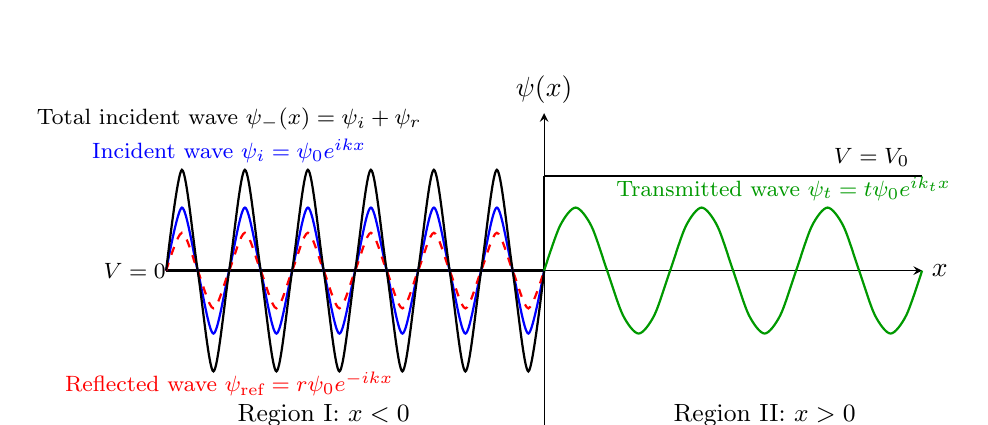
\begin{tikzpicture}[scale=0.8, >=stealth]

                % Axes
                \draw[->] (-6,0) -- (6,0) node[right] {$x$};
                \draw[->] (0,-2.5) -- (0,2.5) node[above] {$\psi(x)$};
                
              
                % Potential step shape (above x-axis)
                \draw[thick] (-6,0) -- (0,0); % left constant
                \draw[thick] (0,0) -- (0,1.5); % vertical step line, for clarity
                \draw[thick] (0,1.5) -- (6,1.5); % right lower step
                \node at (-6.5,0) {\footnotesize $V = 0$};
                \node at (5.2,1.8) {\footnotesize $V = V_0$};
              
                % Incoming wave (blue)
                \draw[domain=-6:0, smooth, thick, blue] plot (\x, {sin(deg(2*pi*\x))});
                \node[blue] at (-5,1.9) {\footnotesize Incident wave $\psi_i = \psi_0 e^{ikx}$};
              
                % Reflected wave (red)
                \draw[domain=-6:0, smooth, thick, red, dashed] plot (\x, {0.6*sin(deg(2*pi*\x))});
                \node[red] at (-5,-1.8) {\footnotesize Reflected wave $\psi_{\text{ref}} = r \psi_0 e^{-ikx}$};
              
                % Total wave (black)
                \draw[domain=-6:0, smooth, thick, black] plot (\x, {sin(deg(2*pi*\x)) + 0.6*sin(deg(2*pi*\x))});
                \node[black] at (-5,2.4) {\footnotesize Total incident wave $\psi_-(x) = \psi_{i} + \psi_{r}$};
              
                % Transmitted wave (green)
                \draw[domain=0:6, smooth, thick, green!60!black] plot (\x, {sin(deg(pi*\x))});
                \node[green!60!black] at (3.8,1.3) {\footnotesize Transmitted wave $\psi_{t} = t \psi_0 e^{ik_t x}$};
              
                % Region labels
                \node at (-3.5,-2.3) {\small Region I: $x < 0$};
                \node at (3.5,-2.3) {\small Region II: $x > 0$};
              
              \end{tikzpicture}
              \caption{$\text { Potential step scattering with } E>V_0 \text { and } V_0>0$}
              \label{fig:scatter_inphase}
        \end{figure}

        one can prove that although the wave function is non-normalized, the total probability total \cref{eq:probability_current} is conserved. First give the three currents of different waves: 
        \begin{align}
            j_i &= \frac{\hbar k}{m} \abs{\psi_0}^2 \\
            j_r &= - \frac{\hbar k}{m} \abs{r}^2 \abs{\psi_0}^2 \\
            j_t &= \frac{\hbar k_t}{m} \abs{t}^2 \abs{\psi_0}^2
        \end{align}
        Then, calculate the total incident probability current and compare this with transmitted probability current,
        \begin{align}
            j_i + j_r &= \frac{\hbar k}{m} \left(1- \abs{r}^2\right) \abs{\psi}^2 = \frac{\hbar k}{m} \frac{4 k k_t}{(k+k_t)^2} \abs{\psi_0}^2 \\
            j_t &= \frac{\hbar k_t}{m} \frac{4k^2}{(k+k_t)^2} \abs{\psi}^2 = j_i+j_r
        \end{align}
        \item $V_0<0: \quad r<0,t>0$\\
        The reflected wave has a phase jump\footnote{which also called a scattering phase} $\delta=\pi$, as shown in \cref{fig:scatter_outphase}. The phase jump comes from our result $r = - \abs{r}$, the condition for current conservation is exactly as same as disscussed above.
        \begin{figure}[h!]
            \centering
            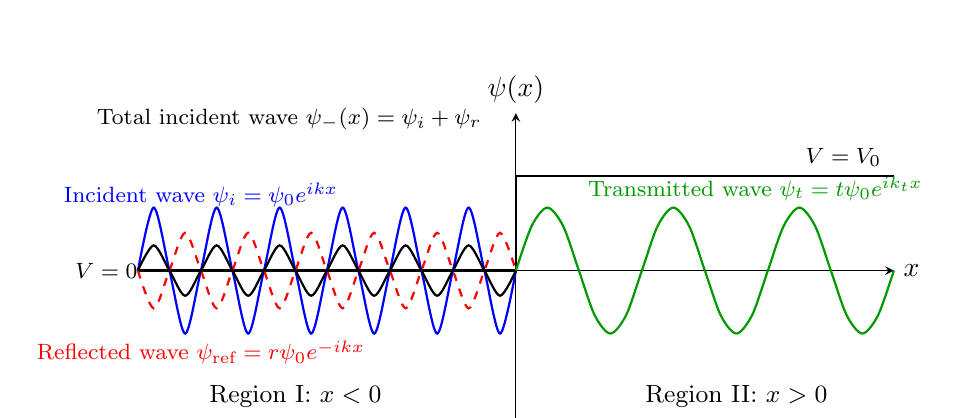
\begin{tikzpicture}[scale=0.8, >=stealth]

                % Axes
                \draw[->] (-6,0) -- (6,0) node[right] {$x$};
                \draw[->] (0,-2.5) -- (0,2.5) node[above] {$\psi(x)$};
                
              
                % Potential step shape (above x-axis)
                \draw[thick] (-6,0) -- (0,0); % left constant
                \draw[thick] (0,0) -- (0,1.5); % vertical step line, for clarity
                \draw[thick] (0,1.5) -- (6,1.5); % right lower step
                \node at (-6.5,0) {\footnotesize $V = 0$};
                \node at (5.2,1.8) {\footnotesize $V = V_0$};
              
                % Incoming wave (blue)
                \draw[domain=-6:0, smooth, thick, blue] plot (\x, {sin(deg(2*pi*\x))});
                \node[blue] at (-5,1.2) {\footnotesize Incident wave $\psi_i = \psi_0 e^{ikx}$};
              
                % Reflected wave (red)
                \draw[domain=-6:0, smooth, thick, red, dashed] plot (\x, {0.6*sin(deg(-2*pi*\x))});
                \node[red] at (-5,-1.3) {\footnotesize Reflected wave $\psi_{\text{ref}} = r \psi_0 e^{-ikx}$};
              
                % Total wave (black)
                \draw[domain=-6:0, smooth, thick, black] plot (\x, {sin(deg(2*pi*\x)) + 0.6*sin(deg(-2*pi*\x))});
                \node[black] at (-3.6,2.4) {\footnotesize Total incident wave $\psi_-(x) = \psi_{i} + \psi_{r}$};
              
                % Transmitted wave (green)
                \draw[domain=0:6, smooth, thick, green!60!black] plot (\x, {sin(deg(pi*\x))});
                \node[green!60!black] at (3.8,1.3) {\footnotesize Transmitted wave $\psi_{t} = t \psi_0 e^{ik_t x}$};
              
                % Region labels
                \node at (-3.5,-2) {\small Region I: $x < 0$};
                \node at (3.5,-2) {\small Region II: $x > 0$};
              
              \end{tikzpicture}
              \caption{$\text { Potential step scattering with } E>V_0 \text { and } V_0<0$}
              \label{fig:scatter_outphase}
        \end{figure}
    \end{itemize}
    \item $E<V_0: \quad k_t = \ii \kappa_t, \; \kappa_t \in \R$, in such case, we can write the wavefunction as 
    \begin{eqnarray}
        \psi_t(x) = t \psi_0 \ee^{\kappa_t x} 
    \end{eqnarray}
    \begin{figure}[h]
        \centering
        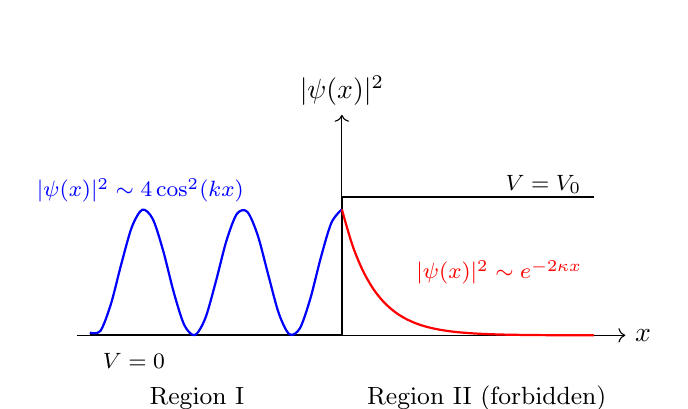
\begin{tikzpicture}[scale=0.8]

    % Define constants
    \def\k{2}          % wave number k
    \def\kk{1}         % decay rate kappa
  
    % Axes
    \draw[->] (-4.2,0) -- (4.5,0) node[right] {$x$};
    \draw[->] (0,0) -- (0,3.5) node[above] {$|\psi(x)|^2$};
  
    % Potential step
    \draw[thick] (-4,0) -- (0,0);     % left side flat
    \draw[thick] (0,0) -- (0,2.2);    % drop
    \draw[thick] (0,2.2) -- (4,2.2);  % right side flat
    \node at (-3.3,-0.4) {\footnotesize $V = 0$};
    \node at (3.2,2.4) {\footnotesize $V = V_0$};
  
    % Vertical dashed line at x=0
    \draw[dashed] (0,0) -- (0,3.2);
  
    % Region labels
    \node at (-2.3,-1) {\small Region I};
    \node at (2.3,-1) {\small Region II (forbidden)};
  
    % Left side: cosine squared wave (standing wave)
    \draw[domain=-4:0, smooth, thick, blue]
      plot (\x, {2*(cos(deg(\k*\x)))^2});
  
    % Right side: exponential decay
    \draw[domain=0:4, smooth, thick, red]
      plot (\x, {2*exp(-2*\kk*\x)});
  
    % Labels
    \node[blue] at (-3.2,2.3) {\footnotesize $|\psi(x)|^2 \sim 4\cos^2(kx)$};
    \node[red] at (2.5,1) {\footnotesize $|\psi(x)|^2 \sim e^{-2\kappa x}$};
  
        \end{tikzpicture}
        \caption{Potential step scattering with $E<V_0$}
        \label{fig:scattering_forbidden}
    \end{figure}
    Now our amplitudes are not real numbers, we can not give it a physical explainations. But if we look at the reflected amplitude, the $\abs{r}^2$ denotes the reflection probability, we can calculate it 
    \begin{eqnarray}
        R = \abs{r}^2 = \abs{\frac{k - \ii \kappa_t}{k + \ii \kappa_t}}^2 = 1
    \end{eqnarray}
    The incident wave reflected completely! There should be no transmitted wave! Now a new question arise, why $\psi_t(x)$ is non-zero expcet $x \ra + \infty$? This means the particle penetrate into the barrier, which is calssical forbidden, but do not propagate. The result is as shown in \cref{fig:scattering_forbidden}.
\end{enumerate}
\subsection{\texorpdfstring{$\delta$}{delta} Function Potential} \label{subsec:delta_potential}




\subsection{1-Dimensional Finite Potential Well: Bounded States}

At \cref{subsec:scattering_state} we disscussed the scattering states, which means that, after the wave incident the potential barrier, the wave was scattered by this potential. Since it is just a one dimensional case, the scattering wave can not behave like the behavior as Compton Scattering in 3-d world. Now we consider a finite potential well to study the bounded state, we will explain what does it mean after we get the full result.

Following the given potential, also as shown in 
\begin{eqnarray}
    V(x) = \begin{cases}
        0, \quad  &0<x<a\\
        V_0, \quad &\mathrm{others}
        \end{cases}
\end{eqnarray}

\begin{figure}[h!]
    \centering
    \begin{tikzpicture}[scale=0.8]
        \draw[->] (-3,0) -- (6,0) node[right] {$x$};
        \draw[->] (0,0) -- (0,4) node[above] {$V(x)$};

        \draw[thick] (-3,3) -- (0,3);
        \draw[thick] (0,0) -- (3,0);
        \draw[thick] (3,3) -- (6,3);
        \draw[thin] (3,0) -- (3,3);
        \node at (1.1,0.4) {\footnotesize $V = 0$};
        \node at (4.1,3.4) {\footnotesize $V = V_0$};
        \node at (-1.1,3.4) {\footnotesize $V = V_0$};
    \end{tikzpicture}
    \caption{The finite potential well}
    \label{fig:finite_potential_well}
\end{figure}

Recall the SE \cref{eq:stationary_x_ode} we get 
\begin{eqnarray}
    \frac{\dd^2 \psi}{\dd x^2} = \frac{2m}{\hbar} \left[ V(x) - E \right] \psi
\end{eqnarray}

As we already disscussed in last section, we need to consider the relation between energy of the particle and the potential, also in following form 
\begin{align}
    k = \begin{cases}
        \frac{\sqrt{2m(E - V_0)}}{\hbar}, \quad E> V_0 \\
        \frac{\ii\sqrt{2m(V_0 - E)}}{\hbar}, \quad E< V_0
    \end{cases}
\end{align}


\newpage
\section{1-Dimensional Harmonic Oscillators: Extension of Hilbert Space}
We condsider the Hamiltonian of a Harmonic Oscillator calssically, 
\begin{eqnarray}
    H = \frac{p^2}{2m} + \frac{1}{2} m \omega^2 x^2
\end{eqnarray}
then move to a quantum condition, i.e., $p \ra \op, x \ra \ox$, and we get the Hamiltonian Operator,
\begin{eqnarray}
    \oH = \frac{\op^2}{2m} + \frac{1}{2} m \omega^2 \ox^2
\end{eqnarray}
The Hamiltonian of Harmonic Oscillator is time-independent and Hermitian, due to \cref{eq:stationary_x_ode,theorem:spectrum_hermitian}, such kind of condition would have a energy eigenvalue function: 
\begin{align}
    \oH \ket{\psi_ \nu^i} = E_ \nu \ket{\psi_ \nu^i} \label{eq:SHO_eigenvalue_equation}
\end{align}
Here we won't study the general wave function in a definite representation, we will talk about it later as we finish the eigenvector and eigenvalue problems. 

\subsection{Eigenvalues of the Hamiltonian}
First we extend our operators $\ox,\op$ to such form: 
\begin{align}
    \oX &= \sqrt{\frac{m \omega}{\hbar}} \ox \\
    \oP &= \frac{1}{\sqrt{m \hbar \omega}} \op
\end{align}
The new commutator is 
\begin{align}
    \comm{\oX}{\oP} = \sqrt{\frac{m \omega}{\hbar}} \cdot \frac{1}{\sqrt{m \hbar \omega}} \comm{\ox}{\op} = \frac{1}{\hbar} \ii \hbar = \ii
\end{align}
Now the Hamiltonian becomes
\begin{align}
    \oH = \frac{\hbar \omega}{2} \left(\oX^2 + \oP^2\right) \label{eq:Hamiltonian_SHO_xp}
\end{align}
Now we shall explain why we construct such a form, since the observables obviously have dimensions\footnote{$\ox:[\mathrm{m}],\op:[\mathrm{m \cdot kg \cdot s^{-1}}]$}. The dimension of $\hbar$ is $[\mathrm{m^2 \cdot kg \cdot s^{-1}}]$, the dimension of $\omega$ is $[\mathrm{s^{-1}}]$, it is easy to see that the new operators have same dimension as we wish.

Now we study more about the new operators, we find the fact $\oX^2 + \oP^2 = \left(\oX - \ii \oP\right) \left(\oX + \ii \oP\right)$, therefor we set, 
\begin{align}
    \a &= \frac{1}{\sqrt{2}} \left(\oX + \ii \oP\right) = \frac{1}{\sqrt{2}} \left( \sqrt{\frac{m \omega}{\hbar}} \ox + \ii \frac{1}{\sqrt{m \hbar \omega}} \op \right)\\
    \adag & = \frac{1}{\sqrt{2}} \left(\oX - \ii \oP\right) = \frac{1}{\sqrt{2}} \left( \sqrt{\frac{m \omega}{\hbar}} \ox - \ii \frac{1}{\sqrt{m \hbar \omega}} \op \right)
\end{align}
Inversly,
\begin{align}
    \ox = \sqrt{\frac{\hbar}{2m\omega}} \left(\adag+ \a\right) \label{eq:ox_as_aadag} \\ 
    \op = \ii \sqrt{\frac{m \hbar \omega}{2}} \left(\adag - \a\right) \label{eq:op_as_aadag}
\end{align}
We can compute the commutator of $\a,\adag$, 
\begin{eqnarray}
    \comm{\a}{\adag} = \frac{1}{2} \comm{\oX + \ii \oP}{\oX + \ii \oP} = \frac{\ii}{2} \comm{\oP}{\oX} - \frac{\ii}{2} \comm{\oX}{\oP} = -\frac{ \ii}{2} \times \ii \times 2 = 1
\end{eqnarray}
Thus we obtain an important relation,
\begin{eqnarray}
    \a \adag = 1 + \adag \a 
\end{eqnarray}
The last term of \rhs is 
\begin{align}
    \adag \a = \frac{1}{2} \left(\oX - \ii \oP\right) \left( \ox + \ii \oP \right) &= \frac{1}{2} \left[\oX^2 + \ii\left( \oX \oP - \oP \oX \right) + \oP^2 \right] = \frac{1}{2} \left( \oX^2 + \oP^2 -1 \right) \\
    &= \frac{1}{2} \left(\oX^2+ \oP^2 + \ii \comm{\oX}{\oP}\right) = \frac{1}{2} = \left(\oX^2 + \oP^2 -1\right) 
\end{align}
Reconsider \cref{eq:Hamiltonian_SHO_xp}, using the result above, we obtain
\begin{align}
    \oH = \hbar \omega \left(\adag \a + \frac{1}{2}\right) = \hbar \omega \left( \a \adag - \frac{1}{2} \right) \label{eq:Hamiltonian_SHO_aadag}
\end{align}
We define a new operator\footnote{Also called Number Operator} as
\begin{align}
    \widehat{N} := \adag \a \label{eq:number_operator}
\end{align}
Now the Hamiltonian becomes,
\begin{align}
    \oH = \hbar \omega \left( \oN + \frac{1}{2} \right)\label{eq:Hamiltonian_SHO_number}
\end{align}
So the eigenvectors of Hamiltonian are definitly the eigenvectors of $\oN$. Before we get to the eigenvectors and eigenvalues, we want also disscuss the commutators related, 
\begin{align}
    \comm{\a}{\a} = \frac{1}{2} \comm{\oX + \ii \oP}{\oX - \ii \oP} = \frac{\ii}{2} \left(\comm{\oX}{\oP} + \comm{\oP}{\oX}\right) = 0 \\
    \comm{\adag}{\adag} = \frac{1}{2} \comm{\oX - \ii \oP}{\oX + \ii \oP} = \frac{\ii}{2} \left(\comm{\oX}{\oP} + \comm{\oP}{\oX}\right) = 0
\end{align}
And also 
\begin{align}
    \comm{\oN}{\a} &= \comm{\adag \a}{\a} = \adag \comm{\a}{\a} + \comm{\adag}{\a} \a = 0 - \a = \a \\
    \comm{\oN}{\adag} &= \comm{\adag \a}{\adag} = \adag \comm{\a}{\adag} + \comm{\adag}{\adag} \a = \adag + 0 = \adag
\end{align}
By \cref{eq:Hamiltonian_SHO_number} we obtain, 
\begin{align}
    \comm{\oH}{\a} = - \hbar \omega \a \\
    \comm{\oH}{\adag} = \hbar \omega \adag
\end{align}
We could define the eigenvalue equation of number state 
\begin{eqnarray}
    \oN \ket{\psi_ \nu^ i} =  \nu\ket{\psi_ \nu^i}
\end{eqnarray}
The eigenvalue equation \cref{eq:SHO_eigenvalue_equation} also, 
\begin{eqnarray}
    \oH \ket{\psi_ \nu ^i} = \left( \nu + \frac{1}{2}\right) \ket{\psi_ \nu^i} 
\end{eqnarray}
Now we study the properties of the eigenvalues and eigenvectors of $\oN$.
\subsubsection{Determination of the Spectrum}
First we disscuss the properties of eigenvalues of $\oN$. We follow a lemma–proof structure to carry out the analysis,
\begin{lemma} \label{lemma:SHO_eigenvalue_nonnegative}
    The Eigenvalues $ \nu$ of the operator $\oN$ are non-negative.
\end{lemma}
\begin{proof}
    Consider an arbitrary eigenvector $\ket{\psi_ \nu^i}$ of $\oN$. Consider the square of norm of the vector $\a \ket{\psi_ \nu^i}$ is non-negative,
    \begin{eqnarray}
        \norm{\a \ketsho}^2 = \brasho \adag \a \ketsho \geq 0
    \end{eqnarray}
    the operator in front of the bra ket is just the number operator. Now, the square of norm is
    \begin{eqnarray}
        \brasho \oN \ketsho = \brasho \nu \ketsho = \nu \braket{\psi_ \nu^i|\psi_ \nu^i} \label{eq:SHO_eigenvalue_norm}
    \end{eqnarray}
    The norm $\braket{\psi_ \nu^i|\psi_ \nu^i}$ is positive. Such that the eigenvalues $\nu \geq 0$
\end{proof}

\begin{lemma} \label{lemma:annihilation_properties}
    Let $\ketsho$ be a (non-zero) eigenvector of $\oN$ with the eigenvalue $\nu$ 
    \begin{enumerate}
        \item If $ \nu = 0$, the ket $\a \ket{\psi_{\nu=0}^i}$ is zero. 
        \item If $ \nu > 0$, the ket $\a \ketsho$ is a non-zero eigenvector of $\oN$ with the eigenvalue $ \nu -1 $
    \end{enumerate}
\end{lemma}

\begin{proof}
    \begin{enumerate}
        \item According to \cref{eq:SHO_eigenvalue_norm}, if $ \nu=0$, $\norm{\ketsho}$ is zero vector. Such that $\nu =0 $ is the eigenvalue of $\oN$, the following holds:
        \begin{eqnarray}
            \a \ket{\psi_0^i} = 0
        \end{eqnarray}
        \item Consider the vector $\a \ket{\psi_ \nu^i}$
        \begin{align}
            \a \ket{\psi_ \nu^i} =& - \comm{\oN}{\a} \ketsho = \a \oN \ketsho - \oN \a \ketsho \notag \\
            =&  \nu \a \ketsho - \oN \a \ketsho \notag \\
            \Ra& \oN \a \ketsho = \left( \nu - 1\right) \a \ketsho
        \end{align}
    \end{enumerate}
\end{proof}

\begin{lemma} \label{lemma:creation_properties}
    Let $\ketsho$ be a (non-zero) eigenvector of $\oN$ of eigenvalue $\nu$, the followings are true 
    \begin{enumerate}
        \item $\adag \ketsho$ is always non-zero. 
        \item $\adag \ketsho$ is an eigenvector of $\oN$ with the eigenvalue $\nu + 1$
    \end{enumerate}
\end{lemma}

\begin{proof}
    \begin{enumerate}
        \item The norm of $\adag \ketsho$ is 
        \begin{align}
            \norm{\adag \ketsho}^2 &= \brasho \a \adag \ketsho \notag \\
            &= \brasho (\adag \a + 1) \ketsho \notag \\ 
            &= \brasho \left(\oN + 1\right) \ketsho \notag \\
            &= \left(\nu + 1\right) \braket{\psi_ \nu^i| \psi_ \nu^i}
        \end{align}
        Due to \cref{lemma:SHO_eigenvalue_nonnegative}, the ket $\adag \ketsho$ always has a non-zero norm and, consequently, is never zero. 
        \item Consider the vector $\adag \ketsho$ 
        \begin{align}
            \adag \ketsho &= \comm{\oN}{\adag} \ketsho = \oN \adag \ketsho - \adag \oN \ketsho \notag \\
            &= \oN \adag \ketsho -  \nu \adag \ketsho \notag \\
            \Ra& \oN \adag \ketsho = \left( \nu + 1\right) \ketsho
        \end{align}
    \end{enumerate}
\end{proof}

Then, we use lemmas above to give the fact that the spectrum of $\oN$ is composed of non-negative integers. We use proof by contradiction, we suppose $ \nu$ is non-integer we can always find an integer $n \geq 0$ such that: 
\begin{eqnarray} 
    n <  \nu < n+1 \label{eq:SHO_hypothesis}
\end{eqnarray}
we can consider a series of vectors, 
\begin{eqnarray}
    \ketsho, \a \ketsho, \dots, \a^n \ketsho
\end{eqnarray}
if we have the p-th vector in this series, this must be non-zero, and its corresponding eigenvalue is $\nu -p$. This is easy to prove by iteration, we won't give the details. But it is true. We now consider the $\a^ n \ketsho$, its corresponding eigenvalue $ \nu - n$, and this is a non-zero vector. Again, $\a^ {n+1} \ketsho$, the corresponding eigenvalue of this ket is $\nu - n - 1$, this should be positive as our \cref{lemma:annihilation_properties}, but as our hypothesis \cref{eq:SHO_hypothesis}, this should be strictly negative. Since they contract each other, we can convince that $\nu$ is integer. As we have defined $\nu$ belongs to a index set. So we can now write it as just $\nu$. Due to \cref{lemma:creation_properties}, the spectrum $\oN$ indeed includes all positive and zero integers. From this we can see check the eigenvalue of $\oH$ again, this should be 
\begin{eqnarray}
    E_n = \left(n+ \frac{1}{2}\right) \hbar \omega
\end{eqnarray}
We could find the energy of the Harmonic Oscillator is quantized and cannot take on any arbirtay value. The ground state now is not 0, but $\hbar \omega/2$.

\subsubsection{Degenracy of the eigenvalue}
When we talking about the eigenvalues of an Operator, it is essential to talk about the degenracy. 

The eigenvectors of $\H$ associated with the eigenvalue $E_0 \hbar \omega/2$, which is, the eigenvectors of $\oN$ associated with the eigenvalue $n=0$, must satisfy the equation: 
\begin{eqnarray}
    \a \ket{\psi_0 ^i} = 0
\end{eqnarray}
To find the degenracy of the ground state, all we must do is see how many linearly independent kets satisfy the equation above. Expand this as 
\begin{eqnarray}
    \frac{1}{\sqrt{2}} \left( \sqrt{\frac{m \omega}{\hbar}} \ox + \frac{\ii}{\sqrt{m \hbar \omega}}\op \right) \ket{\psi_0 ^i} = 0
\end{eqnarray}
Write it in the position representation, this relation becomes: 
\begin{eqnarray}
    \left(\frac{m\omega}{\hbar}\ox + \frac{\dd}{\dd x}\right) \psi_0^i(x) = 0
\end{eqnarray}
The general solution is 
\begin{eqnarray}
    \psi_0^i (x) = A \exp\left(- \frac{1}{2} \frac{m \omega}{\hbar} x^2\right)
\end{eqnarray}
This means the solutions of the equation are propotional to the exponential term. Such that there are no more kets satisfy the differential equation: the ground state is not degenerate. 
Now we check the other states, all what we need to prove is that, if the level $E_n = (n + 1/2)\hbar \omega$ is not degenerate, the level $E_{n+1} = (n+1 + 1/2)\hbar \omega$ is not either, i.e., 
\begin{eqnarray}
    \oN \ketshoizero = n \ketshoizero
\end{eqnarray} 


\subsection{Eigenvectors of the Hamiltonian}
The vector $\ket{\psi_0}$ associated with $n=0$ is the vector which satisfy:
\begin{eqnarray}
    \a \ket{\psi_0} = 0
\end{eqnarray}
It is defined to within a constant factor; we shall assume this is normalized. And it is propotional to $\ket{\psi_1}$,
\begin{eqnarray}
    \ket{\psi_1} = c_1 \adag \ket{\psi_0}
\end{eqnarray}
this is also normalized
\begin{eqnarray}
    \braket{\psi_1|\psi_1} = c_1^* c_1 \bra{\psi_0} \a \adag \ket{\psi_0} = \abs{c_1}^2 \bra{\psi_0} (\adag \a + 1) \ket{\psi_0} = \abs{c_1}^2 =1 
\end{eqnarray}
Such that 
\begin{eqnarray}
    \ket{\psi_1} = \adag \ket{\psi_0}
\end{eqnarray}
similarly we can prove the following: 
\begin{eqnarray}
    \ket{\psi_n} = \frac{1}{\sqrt{n}} (\adag)^n \ket{\psi_0} 
\end{eqnarray}
This just relate some trivial calculation. Won't give it explicitly here.
\subsubsection{Orthonormalization and closure relations}
Since $\H$ is Hermitian, the spectrum of it must consist of a set of eigenvectors which are orthonormal, i.e.
\begin{eqnarray}
    \braket{\psi'_n|\psi_n} = \delta_{n'n}
\end{eqnarray}
Also they are complete sets 
\begin{eqnarray}
    \sum_n \ket{\psi_n} \bra{\psi_n} = \I
\end{eqnarray}
Now we rewrite $\ket{\psi_n} = \ket{n}$, $n$ contains every information we need, we don't need to use $\psi$ to denote it anymore.

\subsubsection{Creation and Annihilation Operators on the eigenvectors}
In the basis of $\basispsi$, the action of the creation and annihilation operators on the kets is given by, 
\begin{align}
    \adag \ket{n} = \sqrt{n} \ket{n+1} \label{eq:Creation_eigenequation} \\
    \a \ket{n} = \sqrt{n} \ket{n-1} \label{eq:Annihilation_eigenequation}
\end{align}
Now we explain, why we call them Creation ($\adag$) and Annihilation ($\a$) Operators, \cref{eq:Creation_eigenequation} shows the creation operator can raise $n$ to $n+1$, like it creates a particle, \cref{eq:Annihilation_eigenequation} shows the annihilation operator can lower $n$ to $n-1$, like it annihilation a particle. 

What is eigenvalue of $\ox$ and $\op$? Using
\begin{eqnarray}
    \ox \ket{n} = \sqrt{\frac{\hbar}{2m \omega}} \left(\adag + \a\right) \ket n = \sqrt{\frac{\hbar}{2m \omega}} \left[\sqrt{n+1}\ket{n+1} + \sqrt{n} \ket{n-1}\right] \\
    \op \ket n = \ii \sqrt{\frac{m \hbar \omega}{2}} \left(\adag - \a\right) \ket n = \ii \sqrt{\frac{m\hbar \omega}{2}} \left[ \sqrt{n+1} \ket{n+1} - \sqrt{n} \ket{n-1} \right]
\end{eqnarray}
Now consider the wavefunction of the state, in position representation, i.e., $\braket{x|n} = \psi_n(x)$, 
\begin{eqnarray} 
    \bra{x} \ox \ket{n} = x \psi_n(x) = \sqrt{\frac{\hbar}{2m \omega}} \left( \sqrt{n+1} \psi_{n+1}(x) + \sqrt{n} \psi_{n-1}(x) \right) \\ 
    \bra{x} \op \ket{n} = - \ii \hbar \frac{\dd}{\dd x} \psi_n(x) = \ii \sqrt{\frac{m \hbar \omega}{2}} \left( \sqrt{n+1} \psi_{n+1}(x) - \sqrt{n} \psi_{n-1}(x) \right)
\end{eqnarray}
Now set $\xi = \sqrt{m \omega/\hbar}x, \alpha = \sqrt{\hbar/ 2m\omega}$. Plug in these into the equation above, we obtain: 
\begin{align*}
    &\sqrt{\frac{\hbar}{m \omega}}\xi \psi_n(\xi) = \sqrt{\frac{\hbar}{2m \omega}} \left( \sqrt{n+1} \psi_{n+1}(\xi) + \sqrt{n} \psi_{n-1}(\xi) \right) \\ 
    \Ra\quad& \xi \psi_n(\xi) = \frac{1}{\sqrt{2}} \left( \sqrt{n+1} \psi_{n+1}(\xi) + \sqrt{n} \psi_{n-1}(\xi) \right) \label{eq:xi_psin} \numberthis \\ 
    & -\sqrt{ m \omega \hbar} \frac{\dd}{\dd \xi}  \psi_n(\xi) = \sqrt{\frac{m \hbar \omega}{2}} \left( \sqrt{n+1} \psi_{n+1}(\xi) - \sqrt{n} \psi_{n-1}(\xi) \right) \\
    \Ra \quad& \psi'_n(\xi) = \frac{1}{\sqrt{2}} \left( \sqrt{n+1} \psi_{n+1}(\xi) - \sqrt{n} \psi_{n-1}(\xi) \right) \label{eq:psin_diff} \numberthis
\end{align*} 
We sum and subtract \cref{eq:xi_psin,eq:psin_diff} and obtain, 
\begin{eqnarray}
    &\psi'_n(\xi) + \xi \psi_n(\xi) - \sqrt{2} \sqrt{n+1} \psi_{n+1}(\xi) = 0 \\
    &\psi'_n(\xi) - \xi \psi_n(\xi) + \sqrt{2} \sqrt{n} \psi_{n-1}(\xi) = 0
\end{eqnarray}
Now we investigate the ground state and first several excited states by using \cref{eq:Creation_eigenequation,eq:Annihilation_eigenequation}
\begin{align*}
    & \bra{x} \a \ket{0} = \frac{1}{\sqrt{2}} \left( \sqrt{\frac{m \omega}{\hbar}}\ox + \ii \frac{1}{\sqrt{m \hbar \omega}} \op \right) \psi_0(x) = 0 \\
    \Ra \quad&\frac{m \omega}{\hbar} x + \frac{\dd}{\dd x} \psi_0(x) = 0 \Ra \psi_0(x) = A \exp\left(-\frac{m \omega }{2 \hbar} x^2\right)
\end{align*}
Now we normalize this 
\begin{eqnarray}
    1 = \int_{-\infty}^{\infty} \dd x \abs{\psi_0(x)}^2 = \abs{A}^2 \int_{-\infty}^{\infty} \dd x \exp\left(-\frac{m \omega }{2 \hbar} x^2\right) = A^2 \sqrt{\frac{\hbar \pi}{m \omega}} \quad \Ra \quad A = \left(\frac{m \omega}{\pi \hbar}\right)^{1/4}
\end{eqnarray}
Also we can also obtain the first and second excited state $\psi_1 = \braket{x|1}, \psi_1 = \braket{x|2}$
\begin{align*}
    \braket{x|1} = \bra{x}\adag \ket{0} = \frac{1}{\sqrt{2}} \left( \sqrt{\frac{m \omega}{\hbar}} x - \ii \frac{1}{\sqrt{m \hbar \omega}} \left(- \ii \hbar \frac{\dd}{\dd x}\right) \right) \psi_0(x) \\
    \braket{x|2} = \frac{1}{\sqrt{2!}}\bra{x}{(\adag)}^2\ket{0} = \frac{1}{\sqrt{2}} \left( \sqrt{\frac{m \omega}{\hbar}} x - \ii \frac{1}{\sqrt{m \hbar \omega}} \left(- \ii \hbar \frac{\dd}{\dd x}\right) \right)^2 \psi_0(x)
\end{align*}
Plug in $\psi_0$ into above, one can obtain, 
\begin{align}
    \psi_1(x) = \sqrt{\frac{2 m \omega}{\hbar}} x \psi_0(x) = \sqrt{\frac{2}{\sqrt{\pi}}} \left(\frac{m \omega}{\hbar}\right)^{3/4}x \exp \left(- \frac{m \omega}{2 \hbar}x^2\right) \\
    \psi_2(x) = \sqrt{\frac{1}{2\sqrt{\pi}}}\left(\frac{m \omega}{\hbar}\right)^{1/4} \left(\frac{2m\omega}{\hbar}x^2-1\right)\exp \left(-\frac{m \omega}{2\hbar}x^2\right)
\end{align}
Then we can also calculate the $\psi_n$
\begin{align}
    \psi_n(x) &= \frac{1}{\sqrt{n!}} \left(\frac{m \omega}{2\hbar}\right)^{n/2} \left(x - \frac{\hbar}{m \omega} \frac{\dd}{\dd x}\right)^n \psi_0(x) \notag \\
    &= \frac{1}{\sqrt{ \sqrt{\pi}2^n n!}} \left(\frac{m \omega}{\hbar}\right)^{\frac{2n+1}{4}}  \left(x - \frac{\hbar}{m \omega} \frac{\dd}{\dd x}\right)^n \exp\left(- \frac{m \omega}{2 \hbar}x^2\right) \label{eq:psin_beforesolution}
\end{align}
NOw we want to seek a general solution of this, we can find the following identities,
\begin{eqnarray}
    \exp\left(- \frac{m \omega}{2 \hbar}x^2\right) \left(x - \frac{\hbar}{m \omega} \frac{\dd}{\dd x}\right)^n \exp\left( \frac{m \omega}{2 \hbar}x^2\right) = (-1)^n \left( \frac{\hbar}{m \omega} \right)^n \frac{\dd^n}{\dd x^n}
\end{eqnarray} 
Use Mathematical Induction to prove this, for $n=1$ is obviously true, assume this is true for $n$, then for $n+1$ 
\begin{align}
    &\exp\left(- \frac{m \omega}{2 \hbar}x^2\right) \left(x - \frac{\hbar}{m \omega} \frac{\dd}{\dd x}\right) \left(x - \frac{\hbar}{m \omega} \frac{\dd}{\dd x}\right)^n \exp\left( \frac{m \omega}{2 \hbar}x^2\right) \\
    =& \exp\left(- \frac{m \omega}{2 \hbar}x^2\right) \left(x - \frac{\hbar}{m \omega} \frac{\dd}{\dd x}\right) \left[ \exp\left( \frac{m \omega}{2 \hbar}x^2\right) (-1)^n \left( \frac{\hbar}{m \omega} \right)^n \frac{\dd^n}{\dd x^n} \right] \\
    =& (-1)^{n+1} \left( \frac{\hbar}{m \omega} \right)^{n+1} \frac{\dd^{n+1}}{\dd x^{n+1}} 
\end{align}
So this is true that we can use it to yield following,
\begin{align}
    &\exp\left( \frac{m \omega}{2 \hbar}x^2\right)\left[\exp\left(-\frac{m \omega}{2 \hbar}x^2\right)\left(x - \frac{\hbar}{m \omega} \frac{\dd}{\dd x}\right)^n \exp\left( \frac{m \omega}{2 \hbar}x^2\right)\right]\exp\left(-\frac{m \omega}{ \hbar}x^2\right) \\
    =& \left(x - \frac{\hbar}{m \omega} \frac{\dd}{\dd x}\right)^n \exp\left(- \frac{m \omega}{2 \hbar}x^2\right) \\
    =& \exp\left( \frac{m \omega}{2 \hbar}x^2\right) (-1)^n \left( \frac{\hbar}{m \omega} \right)^n \frac{\dd^n}{\dd x^n} \exp\left(-\frac{m \omega}{ \hbar}x^2\right) \\
    =& \left( \frac{\hbar}{m \omega} \right)^{n/2} \exp\left(-\frac{m \omega}{2 \hbar}x^2\right) \left[ (-1)^n \exp\left(\frac{m \omega}{ \hbar}x^2\right) \frac{\dd}{\dd \left(\frac{m \omega}{\hbar}x\right)} \exp\left( - \frac{m \omega}{ \hbar}x^2\right) \right] 
\end{align}
Now let $\sqrt{m \omega/\hbar}x = \xi$ we can write above as 
\begin{eqnarray}
    \left( \frac{\hbar}{m \omega} \right)^{n/2} \exp\left(-\frac{m \omega}{2 \hbar}x^2\right) \left[ (-1)^n \ee^ {\xi^2} \frac{\dd^n}{\dd \xi^n} \ee^{-\xi^2} \right] = \left( \frac{\hbar}{m \omega} \right)^{n/2} \exp\left(-\frac{m \omega}{2 \hbar}x^2\right) H_n(\xi)
\end{eqnarray}
Where 
\begin{eqnarray}
    H_n(\xi) = (-1)^n \ee^{\xi^2} \frac{\dd^n}{\dd \xi^n} \ee^{-\xi^2}
\end{eqnarray}
Which we call the Hermitie polynomials, and now we can write the general solution of SHO wavefunction \cref{eq:psin_beforesolution} in terms of the Hermite polynimials as follows:
\begin{align}
    \psi_n(x) &= \frac{1}{\sqrt{\sqrt\pi 2^n n!}} \left(\frac{m\omega}{\hbar}\right)^{(2n+1)/4} \left(\frac{\hbar}{m \omega}\right)^{n/2} \exp\left(- \xi^2/2\right) H_n(\xi) \\
    =& \frac{1}{\sqrt{\sqrt\pi 2^n n!}} \left(\frac{m \omega}{\hbar}\right)^{1/4} \ee^{-\xi^2/2} H_n(\xi)
\end{align}
\newpage

\subsection{Hermite Polynomials}
\subsubsection{Definitions and Properties}
Consider a Gaussian function,
\begin{eqnarray}
    G(z) = \ee^{- z^2}
\end{eqnarray}

\begin{figure}[h!]
    \centering
    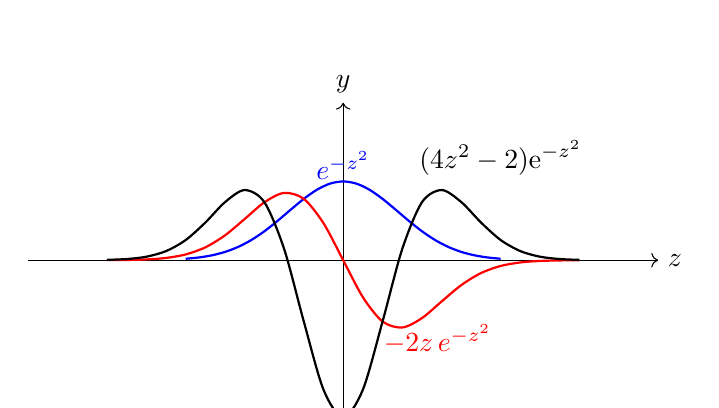
\begin{tikzpicture}
        \draw[->] (-4,0) -- (4,0) node[right] {$z$};
        \draw[->] (0,-2) -- (0,2) node[above] {$y$};
        \draw[domain=-2:2, smooth, variable=\x, blue, thick]
        plot({\x},{exp(-\x*\x)});
        \node[blue] at (0,1.2) {$e^{-z^2}$};

        \draw[domain=-3:3, smooth, variable=\x, red, thick, thick]
        plot ({\x}, {-2*\x*exp(-\x*\x)});
        \node[red] at (1.2,-1) {$-2z\,e^{-z^2}$};

        \draw[domain=-3:3, smooth, variable=\x, black, thick, thick]
        plot ({\x}, {(4*\x*\x - 2)*exp(-\x*\x)});
        \node[black] at (2,1.3) {$(4z^2-2)\ee^{-z^2}$};
    \end{tikzpicture}
    \caption{Diagram of Gaussian Function and the first, second order derivatives.}
    \label{fig:Gaussian}
\end{figure}

The first two orders of derivatives are 
\begin{align}
    G'(z) = - 2 z \ee^{-z^2} \\
    G''(z) = (4z^2-2) \ee^{-z^2}
\end{align}

The n-th order derivative is 
\begin{eqnarray}
    G^{(n)} (z) = (-1)^n H_n(z) \ee^{-z^2}
\end{eqnarray}
Where $H_n(z)$ is the n-th Polynomials of $z$. We can use Mathematical Induction to prove this, for $n=1,2$, the euqation above is obviously true, now we assume it holds for $n-1$ either, 
\begin{eqnarray}
    G^{(n-1)}(z) = (-1)^{n-1} H_{n-1} (z) \ee^{-z^2} 
\end{eqnarray}
Take derivative of this 
\begin{eqnarray}
    G^{(n)}(z) = (-1)^n \left(2z- \frac{\dd}{\dd z}\right) H_{n-1}(z) \ee^{-z^2}
\end{eqnarray}
We can find
\begin{eqnarray}
    H_n(z) = \left(2z-\frac{\dd}{\dd z}\right) H_{n-1}(z)
\end{eqnarray}
We can by this define \emph{Hermitian Polynomials}
\begin{eqnarray}
    H_n(z)=(-1)^n \mathrm{e}^{z^2} \frac{\mathrm{~d}^n}{\mathrm{~d} z^n} \mathrm{e}^{-z^2}
\end{eqnarray}

\newpage


































































































\chapter{General Angular Theory in Quantum Mechanics}

\section{Angular Momentum}

\subsection{From Classical to Quantum}
In classical mechanics, we define angular momentum as 
\begin{eqnarray}
    \mathbf{l} = \mathbf{x} \times \mathbf{p} 
\end{eqnarray}
In component form: 
\begin{eqnarray}
    l_i = \epsilon_{ijk}x_j p_k
\end{eqnarray}
The Possion bracket is 
\begin{eqnarray}
    \{ l_x,l_y \} = \epsilon_{ijk} l_k
\end{eqnarray}
The three components form $\mathfrak{so}(3)$ of Lie algebra. Now we could expand this into Quantum cases, i.e. substitude Possion braket by Commutator, and add $i \hbar$ on the r.h.s.
\begin{eqnarray}
    [ \oL_i,\oL_j ]= \ii \hbar \epsilon_{ijk} \oL_k \label{com_rel_of_L}
\end{eqnarray}
in component form
\begin{eqnarray}
    \oL_i = \epsilon_{ijk} \ox_j \op_k \label{eq:component_L}
\end{eqnarray}
Now we check if this operator is adjoint. Due to the component form \cref{eq:component_L}
\begin{align*}
    \oL_i^ \dag &= \epsilon_{ijk} \ox_j^\dag \op_k^\dag 
\end{align*}
Since $\ox$ and $\op$ are all self-adjoint, $\oL$ is also self-adjoint, i.e.
\begin{eqnarray}
    \braket{\Psi|\oL\Psi} = \braket{\oL \Psi|\Psi} 
\end{eqnarray}
The square of the angular momentum $\oL$ is 
\begin{eqnarray}
    \abs{\boL}^2 \equiv \oL_x ^2+ \oL_y^2 +\oL_z^2 \label{dfn:lsquare}
\end{eqnarray}
Which is also called \textit{Casimir Operatpr}. It is also adjoint. What is the relation between this and its components, namely the commutator $\left[ \abs{\oL^2},\oL_i \right]$:
\begin{align*}
    \left[ \abs{\boL^2},\oL_i \right] &= \left[ \sum_{i=x,y,z} \oL_i^2,\oL_j \right] = \sum_{i=x,y,z} \left[ \oL_i^2,\oL_j \right] = \sum_{i=x,y,z} \left( \oL_i \left[\oL_i,\oL_j  \right] + \comm{\oL_i}{\oL_j} \oL_i \right) \\
    &=\sum_{i=x,y,z} \left( \oL_i \ii \hbar \epsilon_{ijk} \oL_k + \ii \hbar \epsilon_{ijk} \oL_k \oL_i \right) = \ii \hbar \sum_{i=x,y,z} \varepsilon_{ijk} \anticomm{\oL_i}{\oL_k} \numberthis \label{eq:commutator_Lsquare_L}
\end{align*}
Before actually calculate the result, we need to review some properties of tensors, i.e. symmetry tensor and antisymmetry tensor.
\begin{itemize}
    \item \textbf{Symmetry tensor:} $\mathcal{T}_{ij} = \mathcal{T}_{ji}$
    \item \textbf{Antisymmetry tensor:} $\mathcal{L}_{ijk} = -\mathcal{L}_{jik}$
\end{itemize}
We can prove that we have the following theorem:
\begin{theorem}
    The contraction of an antisymmetric tensor with a symmetric tensor over the same indices is identically zero.
    \begin{eqnarray}
        \mathcal{T}_{ij} \mathcal{L}_{ijk} = 0( \forall i=j,j=k,i=k \quad\mathcal{L}_{ijk}=0)
    \end{eqnarray}
\end{theorem} \label{s}

Now if we consider \cref{eq:commutator_Lsquare_L}, we can regard the anticommutator as a rank-2 symmetry tensor, and we already know that $\varepsilon_{ijk}$ is antisymmetry. Hence we can apply the Theorem \ref{s} to get the result: $ \left[ \abs{\boL^2},\oL_i \right] = 0$. Namely, $\boL^2$ commutes with the components of $\boL$.

Then a question appears, what does it mean of these commutative relations? In Chapter 2 we discussed the meaning of measurement in Quantum Mechanics. A fact is that the order of measurement is the order of operator application. If two operators commute with each other, we call the two measurements are compatiable. \cref{com_rel_of_L} told us the components of angular momentum operator are not commutative which means we can not measure the 3 directions simultaneously.
But we can measure the $\boL^2$ and any of the component at same time.

\section{General Theory of Angular Momentum}

\subsection{Definition and notations}

Instead of using the components $\oL_x$ and $\oL_y$ of the angular momentum $\mathrm{\oL}$ for general cases and study their common eigenvectors.
\begin{definition}{General Agular Momentum}
    \begin{align}
        \oL_+ & = \oL_x + \ii \oL_y \label{dfn:l+}\\
        \oL_- &= \oL_x - \ii \oL_y \label{dfn:l-}
    \end{align}
\end{definition}
These are similar to the creation and annihilation operator of the hramonic oscillator, $\oL_+$ and $\oL_-$ are not Hermitian: but they are adjoints of each other, i.e. $\oL_+^ \dag =\oL_-$. Now we can disscuss the commutation relations: 
\begin{itemize}
    \item \begin{align*}
        \comm{\oL_z}{\oL_+} = \comm{\oL_z}{\oL_x + \ii \oL_y} = \comm{\oL_z}{\oL_x} + \ii \comm{\oL_z}{\oL_y} = \ii \hbar \oL_y + \hbar \oL_x = \hbar \oL_+ 
    \end{align*}
    \item \begin{eqnarray*}
        \comm{\oL_z}{\oL_-} = \comm{\oL_z}{\oL_x - \ii \oL_y} = \comm{\oL_z}{\oL_x} + \ii \comm{\oL_z}{\oL_y} = \ii \hbar \oL_y -\hbar \oL_x = - \hbar \oL_- \label{eq:comm_lz_l-}
    \end{eqnarray*}
    \item \begin{align*}
        \comm{\oL_+}{\oL_-} &= \comm{\oL_x + \ii \oL_y}{\oL_x - \ii \oL_y} = \comm{\oL_x}{\oL_x} - \ii \comm{\oL_x}{\oL_y} -+\ii \comm{\oL_y}{\oL_x} - \comm{\oL_y}{\oL_y} \\
        &= -\ii \ii \hbar \oL_z - \ii \ii \hbar \oL_z = 2 \hbar \oL_z
    \end{align*}
    \item \begin{align*}
        \comm{\oL^2}{\oL_+} = \comm{\oL^2}{\oL_x} + \ii \comm{\oL^2}{\oL_y} = 0 \quad \comm{\oL^2}{\oL_-} = \comm{\oL^2}{\oL_x} - \ii \comm{\oL^2}{\oL_y} = 0 
    \end{align*}
\end{itemize}

Then we can conclude by following 
\begin{tcolorbox}
    \begin{gather}
        \comm{\oL_z}{\oL_+} = \hbar \oL_+ \\
        \comm{\oL_z}{\oL_-} = - \hbar \oL_-\\
        \comm{\oL_+}{\oL_-} = 2 \hbar \oL_z \\
        \comm{\oL^2}{\oL_+} = \comm{\oL^2}{\oL_-} = \comm{\oL^2}{\oL_z} = 0
    \end{gather}
\end{tcolorbox}
We can compute the the product $\oL_- \oL_+$ and $\oL_+ \oL_-$
\begin{align*}
    \oL_+ \oL_- &= \left( \oL_x + \ii \oL_y \right) \left( \oL_x - \ii \oL_y \right) \\
    &= \oL_x^2 + \oL_y^2 - \ii \comm{\oL_x}{\oL_y} \\
    &= \oL_x^2 + \oL_y^2 + \hbar \oL_z \label{eq:l+l-} \numberthis \\
    \oL_- \oL_+ &= \left(\oL_x - \ii \oL_y\right) \left( \oL_x + \ii \oL_y \right)\\
    &= \oL_x^2 + \oL_y^2 + \ii \comm{\oL_x}{\oL_y} \\
    &= \oL_x^2 + \oL_y^2 - \hbar \oL_z \label{eq:l-l+} \numberthis 
\end{align*}
Plug in \cref{eq:l+l-,eq:l-l+} into \cref{dfn:lsquare} we obtain:
\begin{align}
    \oL_+ \oL_- = \oL^2 -\oL_z^2 + \hbar \oL_z \\
    \oL_- \oL_+ = \oL^2 -\oL_z^2 - \hbar \oL_z
\end{align}
Sum the two above, we obtain:
\begin{eqnarray}
    \oL^2 = \frac{1}{2} \left( \oL_+ \oL_- + \oL_- \oL_+ \right) + \oL_z^2
\end{eqnarray}

\subsubsection{\texorpdfstring{Commutative Relation between $\oL$ and $\ox,\op$}{Commutative Relation between L and xp}}
Now we give the commutator $\comm{\oL_i}{\ox_j}$
\begin{align}
    \comm{\oL_i}{\ox_j} &= \comm{\epsilon_{ikl} \ox_k \op_l  }{\ox_j}\notag \\
    &= \epsilon_{ikl} (\ox_k\comm{\op_l}{\ox_j} + \underbrace{\comm{\ox_k}{\ox_j}}_{0} \op_l) \notag \\
    &= -\ii \hbar \epsilon_{ikl} \ox_k \delta_{lj} =- \ii \hbar \epsilon_{ikj} \ox_k \notag \\
    &= \ii \hbar \epsilon_{ijk} \ox_k
\end{align}
Also $\comm{\oL_i}{\op_j}$
\begin{align*}
    \comm{\oL_i}{\op_j} &=\epsilon_{ikl} \comm{\ox_k \op_l}{\op_j} = \epsilon_{ikl} \comm{\ox_k}{\op_j} \op_l  \\
    &= \ii \hbar \epsilon_{ikl} \delta_{kj} \op_l = \ii \hbar \epsilon_{ijk} \op_l \numberthis
\end{align*}

\subsection{\texorpdfstring{Eigenvalues of $\oL^2$ and $\oL_z$}{Eigenvalues of L² and Lz}}

One can verify that the matrix element $\bra{\psi}\oL^2 \ket{\psi}$ is positive or zero: 
\begin{align}
    \bra{\psi}\oL^2 \ket{\psi} = \bra{\psi}\oL_x^2 \ket{\psi} + \bra{\psi}\oL_y^2 \ket{\psi}+\bra{\psi}\oL_z^2 \ket{\psi} =\norm{\oL_x \ket{\psi}}^2 + \norm{\oL_y \ket{\psi}}^2 + \norm{\oL_z \ket{\psi}}^2 \geq 0
\end{align}
We suppose the eigenvalues of $\oL^2$ in the form $l(l+1)\hbar^2$, with the convention: $l\geq0$. The reason why we choose such kind of form is that $\oL$ has the dimension of $\hbar$ and then $\oL^2$ necessarily of the form $\lambda \hbar^2$, where $\lambda$ is a dimensionless number. And we want a non-negative $\lambda$, $l(l+1)$ can determines $\lambda$ with $l$ uniquely.

Also for the eigenvalues of $\oL_z$, which have the same dimensions as $\hbar$, they are traditionally written $m \hbar$, where $m$ is a diemnsionless number. Then the eigenvalue equation for $\oL^2$ and $\oL_z$
\begin{tcolorbox}{Eigenvalue equation for $\oL^2$ and $\oL_z$:}
    \begin{align}
        \oL^2 \ket{k,l,m} &= l(l+1)\hbar^2 \ket{k,l,m}\\
        \oL_z \ket{k,l,m}& = m \hbar \ket{k,l,m}
    \end{align}
\end{tcolorbox}
Now we can disscuss the properties of eigenvalues.

\begin{lemma} \label{lemma:-l<=m<=l}
    If $l(l+1)\hbar^2$ and $m \hbar$ are the eigenvalues of $\oL^2$ and $\oL_z$ associated with the common eigenvector $\ket{k,l,m}$, then $l$ and $m$ satisfy the inequality: 
    \begin{align}
        -l \leq m \leq l
    \end{align}
\end{lemma}
\begin{proof}
    We consider the matrix element $\bra{k,l,m} \oL_- \oL_+ \ket{k,l,m}$, which is non-negative since $\oL_+ \ket{k,l,m}$ is a vector in Hilbert space. Plug in the expression of $\oL_- \oL_+$, we have:
    \begin{align*}
        \bra{k,l,m} \oL_- \oL_+ \ket{k,l,m} &= \bra{k,l,m} \left( \oL^2 -\oL_z^2 - \hbar \oL_z \right) \ket{k,l,m} \\
        &= \left[ l(l+1) - m^2 - m \right] \hbar^2 \geq 0
    \end{align*}
    Rearranging the inequality , we obtain:
    \begin{align*}
        l(l+1) - m^2 - m &\geq 0\\
        (l - m)(l + m + 1) &\geq 0
    \end{align*}
    Since $l + m + 1 > 0$, we have $l - m \geq 0$, i.e. $m \leq l$. Similarly, considering the matrix element $\bra{k,l,m} \oL_+ \oL_- \ket{k,l,m}$,
    \begin{align}
        \bra{k,l,m} \oL_+ \oL_- \ket{k,l,m} &= \bra{k,l,m} \left( \oL^2 -\oL_z^2 + \hbar \oL_z \right) \ket{k,l,m} \\
        &= \left[ l(l+1) - m^2 + m \right] \hbar^2 \geq 0   \label{eq:l+l-positve}
    \end{align} 
    we can prove that $-l \leq m$. Combining these two inequalities, we conclude that $-l \leq m \leq l$.
\end{proof}

\begin{lemma} \label{lemma:l-}
    Let $\ket{k,l,m}$ be an eigenvector of $\oL^2$ and $\oL_z$ with eigenvalues $l(l+1)\hbar^2$ and $m \hbar$, respectively. 
    \begin{enumerate}
        \item If $m=-l$, $\oL_- \ket{k,l,-l} = 0$.
        \item If $m> -l$, $\oL_- \ket{k,l,m}$ is a non-null eigenvector of $\oL^2$ and $\oL_z$ with the eigenvalues $l(l+1)\hbar^2$ and $(m-1)\hbar$
    \end{enumerate}
\end{lemma}
\begin{proof}
    \begin{enumerate}
        \item According to the previous lemma, the square of the norm of the vector $\oL \ket{k,l,m}$ is equal to $\hbar^2[l(l+1)-m(m-1)]$ and therefore vanishes when $m= -l$. Since the norm of a vactor is zero iff the vector is null-vector, we can conclude that all vectors $\oL_-\ket{k,l,-l}$ are null-vectors:
        \begin{align}
            m=-l=0 \implies \oL_- \ket{k,l,-l} = 0
        \end{align} And we can find vice versa: 
        \begin{align}
            \oL_- \ket{k,l,m} = 0 \implies m=-l \label{eq:m=-l}
        \end{align}
        Apply $\oL_+$ act on the both sides of \cref{eq:m=-l}, we have:
        \begin{align*}
            \oL_+ \oL_- \ket{k,l,m} = \hbar^2 [l(l+1) - m(m-1)] \ket{k,l,m} = \hbar^2 [l(l+1) - m(m-1)] \ket{k,l,m} = 0  \label{eq:l+l-0} \numberthis
        \end{align*}
        Since $\ket{k,l,m}$ is non-null, we have $l(l+1) - m(m-1) = 0$. Rearranging this equation, we obtain:
        \begin{align*}
            (l + m)(l - m + 1) = 0
        \end{align*}
        such that $l + m = 0$ or $l - m + 1 = 0$. The second case is impossible since it would imply $m = l + 1 > l$, which contradicts the previous lemma. Therefore, we must have $l + m = 0$, i.e. $m = -l$.
        \item Due to \cref{eq:l+l-positve}, when $m>-l$, the norm of the vector $\oL_- \ket{k,l,m}$ is non-zero, i.e. $\oL_- \ket{k,l,m}$ is a non-null vector. Now we check if it is an eigenvector of $\oL^2$ and $\oL_z$:
        \begin{itemize}
            \item FIrst we check $\oL^2$, since $\comm{\oL^2}{\oL_-} = 0$, we have:
            \begin{align*}
                \oL^2 \left( \oL_- \ket{k,l,m} \right) &= \oL_- \left( \oL^2 \ket{k,l,m} \right) = l(l+1)\hbar^2 \left( \oL_- \ket{k,l,m} \right)
            \end{align*}
            This relation expresses the fact that $\oL_- \ket{k,l,m}$ is an eigenvector of $\oL^2$ with eigenvalue $l(l+1)\hbar^2$.
            \item Now we check $\oL_z$, by commutator $\comm{\oL_z}{\oL_-} = - \hbar $, we apply this to $\ket{k,l,m}$
            \begin{align}
                &\comm{\oL_z}{\oL_-} \ket{k,l,m} = - \hbar \oL_- \ket{k,l,m} \notag \\
                \implies &\oL_z \left( \oL_- \ket{k,l,m} \right) &= \oL_- \left( \oL_z \ket{k,l,m} \right) - \hbar \left( \oL_- \ket{k,l,m} \right) \notag \\
                &= m \hbar \left( \oL_- \ket{k,l,m} \right) - \hbar \left( \oL_- \ket{k,l,m} \right) \notag \\
                &= (m-1) \hbar \left( \oL_- \ket{k,l,m} \right) \numberthis \label{eq:lz_l-}
            \end{align}
            $\oL_- \ket{k,l,m}$ is therefore an eigenvector of $\oL_z$ with eigenvalue $(m-1)\hbar$.
        \end{itemize}
    \end{enumerate}
\end{proof}

\begin{lemma} \label{lemma:l+}
    Let $\ket{k,l,m}$ be an eigenvector of $\oL^2$ and $\oL_z$ with eigenvalues $l(l+1)\hbar^2$ and $m \hbar$, respectively. 
    \begin{enumerate}
        \item If $m=l$, $\oL_+ \ket{k,l,l} = 0$.
        \item If $m< l$, $\oL_+ \ket{k,l,m}$ is a non-null eigenvector of $\oL^2$ and $\oL_z$ with the eigenvalues $l(l+1)\hbar^2$ and $(m+1)\hbar$
    \end{enumerate}
\end{lemma}
\begin{proof}
    \begin{enumerate}
        \item According to the norm of $\oL_+\ket{k,l,m}$ is zero if $m=l$. Such that 
        \begin{align}
            m=l \implies \oL_+ \ket{k,l,l} = 0
        \end{align}
        And vice versa, if $\oL_+ \ket{k,l,m} = 0$, we can apply $\oL_-$ on both sides and obtain:
        \begin{align*}
            \oL_- \oL_+ \ket{k,l,m} = \hbar^2 [l(l+1) - m(m+1)] \ket{k,l,m} = 0
        \end{align*}
        \item If $m<l$, the norm of $\oL_+ \ket{k,l,m}$ is non-zero, such that it is a non-null vector. Now we check if it is an eigenvector of $\oL^2$ and $\oL_z$:
        Since $\comm{\oL^2}{\oL_+} = 0$, we have:
            \begin{align*}
                \oL^2 \left( \oL_+ \ket{k,l,m} \right) &= \oL_+ \left( \oL^2 \ket{k,l,m} \right) = l(l+1)\hbar^2 \left( \oL_+ \ket{k,l,m} \right)
            \end{align*}
        This relation expresses the fact that $\oL_+ \ket{k,l,m}$ is an eigenvector of $\oL^2$ with eigenvalue $l(l+1)\hbar^2$. Similarly, by commutator $\comm{\oL_z}{\oL_+} = \hbar \oL_+$, we apply this to $\ket{k,l,m}$
        \begin{align}
            &\comm{\oL_z}{\oL_+} \ket{k,l,m} = \hbar \oL_+ \ket{k,l,m} \notag \\
            \implies &\oL_z \left( \oL_+ \ket{k,l,m} \right) = \oL_+ \left( \oL_z \ket{k,l,m} \right) + \hbar \left( \oL_+ \ket{k,l,m} \right) \notag \\
            &= m \hbar \left( \oL_+ \ket{k,l,m} \right) + \hbar \left( \oL_+ \ket{k,l,m} \right) \notag \\
            &= (m+1) \hbar \left( \oL_+ \ket{k,l,m} \right) \numberthis \label{eq:lz_l+}
        \end{align}
    \end{enumerate}
\end{proof}

\subsection{Spectrum of \texorpdfstring{$\oL^2$}{L²} and \texorpdfstring{$\oL_z$}{Lz}}

By the given 3 lemmas above, we are now able to determine the spectrum of $\oL^2$ and $\oL_z$. From \cref{lemma:-l<=m<=l}, we know that $-l<m<l$. It is therefore certain that a positive or zero integer $p$ exists such that: 
\begin{align}
    -l \leq m-p < -l+1
\end{align}
Consider the series of vectors: 
\begin{align}
    \ket{k,l,m}, \oL_- \ket{k,l,m}, \oL_-^2 \ket{k,l,m}, \ldots, \oL_-^p \ket{k,l,m}
\end{align}
\large
\emph{I am done. Ignore this part and show the answer directly. Maybe I will finish this when I’m in the mood.
}
\begin{align}
    \oL_z \ket{k,l,m} &= m\hbar \ket{k,l,m} \\
    \oL^2 \ket{k,l,m} &= l(l+1)\hbar^2 \ket{k,l,m} \\
    \oL_+ \ket{k,l,m} &= \hbar \sqrt{j(j+1)-m(m+1)} \ket{k,l,m+1} \\
    \oL_- \ket{k,l,m} &= \hbar \sqrt{j(j+1)-m(m-1)} \ket{k,l,m-1}
\end{align}
The allowed values of $l$ and $m$ are 
\begin{align}
    l &= 0, \frac{1}{2}, 1, \frac{3}{2}, 2, \ldots \\
    m &= -l, -l+1, \ldots, l-1, l
\end{align}


\section{Eigenfunction of Angular Momentum Operators}

The eigenfunction of angular momentum operators are usually expressed in the spherical coordinate system $(r,\theta,\phi)$. The relations between Cartesian coordinates and spherical coordinates are given in Appendix. \ref{sec:AngularMomentum_SphericalCoord}, by this one can obtain the operators $\oL_z, \oL^2,\oL_{\pm}$ in spherical coordinates: 
\begin{align}
    \oL_z &= - \ii \hbar \pdv{}{\phi} ,\\
    \oL^2 &= - \hbar^2 \left[\frac{1}{\sin \theta} \pdv{}{\theta} \left(\sin \theta \pdv{}{\theta} + \frac{1}{\sin^2 \theta} \frac{\pp^2}{\pp \phi^2}\right)\right], \\
    \oL_{\pm} & = \oL_x \pm \ii \oL_y = \pm \hbar \ee^{\pm \ii \phi} \left(\pdv{}{\theta} \pm \ii \cot \theta \pdv{}{\phi}\right)
\end{align}

It is straightforward that $\oL_z$ and $\oL^2$ depend only on the angles $\theta$ and $\phi$, such that their eigenvectors depend only on $\theta$ and $\phi$. Denoting their joint eigenstates by 
\begin{align}
    \braket{\theta,\phi|l,m} = \Ylm (\theta,\phi)
\end{align}
where $\Ylm (\theta, \phi)$ are continuous functions of $\theta$ and $\phi$, called \textit{spherical harmonics}. Such that the eigenvalue equations for $\oL_z$ and $\oL^2$ read as 
\begin{align}
    \oL_z \Ylm (\theta,\phi) &= m \hbar \Ylm (\theta,\phi) \label{eq:eigen_lz_spherical}\\
    \oL^2 \Ylm (\theta,\phi) &= l(l+1) \hbar^2 \Ylm (\theta,\phi) \label{eq:eigen_lsquare_spherical}
\end{align}

Moreover, $\oL_z$ depends only on $\phi$, this suggests that the spherical harmonics are seperable in $\theta$ and $\phi$. We try the ansatz:
\begin{align}
    \Ylm (\theta,\phi) = \Theta_l^m(\theta) \Phi_l^m(\phi) \label{eq:seperation_Ylm}
\end{align}
One ascertains that 
\begin{align}
    \oL_{\pm} \Ylm (\theta,\phi) = \hbar \sqrt{l(l+1) - m(m \pm 1)} Y_l^{m \pm 1} (\theta,\phi)
\end{align}

\subsection{Eigenfunction of \texorpdfstring{$\oL_z$}{Lz}}
Inserting \cref{eq:seperation_Ylm} into \cref{eq:eigen_lz_spherical}, one can obtain:
\begin{align}
    \oL^z \Ylm (\theta,\phi) &= - \ii \hbar \pdv{}{\phi} \left( \Theta_l^m(\theta) \Phi_l^m(\phi) \right) = - \ii \hbar \Theta_l^m(\theta) \pdv{\Phi_l^m(\phi)}{\phi} \notag \\
    &= m \hbar \Theta_l^m(\theta) \Phi_l^m(\phi) \notag \\
    \implies &\pdv{\Phi_l^m(\phi)}{\phi} = \ii m \Phi_l^m(\phi) 
\end{align}
Since now the equation has nothing to do with $l$, one can simply write $\Phi_m(\phi)$ instead of $\Phi_l^m(\phi)$. The solution of the above equation is:
\begin{align}
    \Phi_m(\phi) = \frac{1}{\sqrt{2 \pi}} \ee^{\ii m \phi}
\end{align}
where the normalization constant $\frac{1}{\sqrt{2 \pi}}$ is determined by the normalization condition:
\begin{align}
    \int_0^{2 \pi} \Phi^*_{m'} (\phi) \Phi_m(\phi) \dd \phi = \delta_{m,m'}
\end{align}
As $\phi$ is the azimuthal angle, it is periodic with period $2 \pi$. Therefore, the eigenfunction $\Phi_m(\phi)$ must satisfy the periodic boundary condition:
\begin{align}
    \Phi_m(\phi) = \Phi_m(\phi + 2 \pi)
\end{align}
This condition requires that $m$ must be an integer, i.e. $m = 0, \pm 1, \pm 2, \ldots$. And we have already know the range of $m$ from \cref{lemma:-l<=m<=l}, such that for a given $l$, $m$ can take the values:
\begin{align}
    m = -l, -l+1, \ldots, l-1, l
\end{align} 
which means that $l$ must be either an integer, i.e. the expectation value of angular momentum is quantized in unit of $\hbar$.

\subsection{Eigenfunction of \texorpdfstring{$\oL^2$}{L²}}
The partial term of spherical harmonics $\Phi_m(\phi)$ has been determined. Inserting this into \cref{eq:eigen_lsquare_spherical} and using \cref{eq:seperation_Ylm}, one can obtain:
\begin{align}
    \oL^2 \Ylm (\theta,\phi) &= - \hbar^2 \left[ \frac{1}{\sin \theta} \pdv{}{\theta} \left( \sin \theta \pdv{}{\theta} \left( \Theta_l^m(\theta) \Phi_m(\phi) \right) \right) + \frac{1}{\sin^2 \theta} \frac{\pp^2}{\pp \phi^2} \left( \Theta_l^m(\theta) \Phi_m(\phi) \right) \right] \notag \\
    &= - \hbar^2 \left[ \frac{1}{\sin \theta} \pdv{}{\theta} \left( \sin \theta \pdv{\Theta_l^m(\theta)}{\theta} \Phi_m(\phi) \right) + \frac{1}{\sin^2 \theta} \Theta_l^m(\theta)  \frac{\pp^2 \Phi_m(\phi)}{\pp \phi^2}  \right] \notag \\
    &= - \hbar^2 \left[  \frac{1}{\sin \theta}  \frac{\dd}{\dd \theta} \left( \sin \theta  \frac{\dd \Theta_l^m(\theta)}{\dd \theta}  \right)  - \frac{m^2}{\sin^2 \theta}  \Theta_l^m(\theta)  \right]  \Phi_m(\phi)  \notag \\
    &= l(l+1) \hbar^2  \Theta_l^m(\theta)  \Phi_m(\phi)  \notag \\
    &=\frac{1}{\sqrt{2 \pi}}  l(l+1) \hbar^2 \Theta_l^m(\theta)  \ee^{\ii m \phi} \label{eq:theta_equation_intermediate}
\end{align}
which, after eliminating the $\phi-$dependence, reduces to the following ordinary differential equation for $\Theta_l^m(\theta)$:
\begin{align}
    \frac{1}{\sin \theta}  \frac{\dd}{\dd \theta} \left( \sin \theta  \frac{\dd \Theta_l^m(\theta)}{\dd \theta}  \right)  + \left[ l(l+1) - \frac{m^2}{\sin^2 \theta} \right]  \Theta_l^m(\theta) = 0 \label{eq:theta_equation}
\end{align}
This equation is know as the \emph{Legendre differential equation}. Its solutions can be expressed in terms of the \emph{associated Legendre functions} $P_l^m(\cos \theta)$:
\begin{align}
    \Theta_l^m(\theta) = C_{lm} P_l^m(\cos \theta) \label{eq:Theta_solution}
\end{align}
The definition of associated Legendre functions is given in Appendix. \ref{sec:AssociatedLegendreFunctions}. The normalization constant $C_{lm}$ can be determined by the normalization condition of spherical harmonics:
\begin{align}
    \braket{l',m'|l,m} = \int_0^{2 \pi} \dd \phi \int_0^{\pi} \sin \theta \dd \theta {\ylm{l}{m}}^* (\theta,\phi) Y_{l'}^{m'} (\theta,\phi) &= \delta_{l,l'} \delta_{m,m'} 
\end{align}
By solving this integral, one can obtain:
\begin{align}
    C_{lm} = (-1)^m \sqrt{\frac{(2l+1)}{4 \pi} \frac{(l-m)!}{(l+m)!}}
\end{align}
Finally, the spherical harmonics $\Ylm (\theta,\phi)$ can be expressed as:
\begin{align}
    \Ylm (\theta,\phi) = (-1)^m \sqrt{\frac{(2l+1)}{4 \pi} \frac{(l-m)!}{(l+m)!}} P_l^m(\cos \theta) \ee^{\ii m \phi} \label{eq:spherical_harmonics}
\end{align}
Such that the eigenvalue equations for $\oL^2$ and $\oL_z$ in spherical coordinates have been solved completely. Conclude the results in a tcolorbox:
\begin{tcolorbox}{Eigenvalue equations for $\oL^2$ and $\oL_z$ in spherical coordinates:}
    \begin{align}
        \oL^2 \Ylm (\theta,\phi) &= l(l+1) \hbar^2 \Ylm (\theta,\phi) \\
        \oL_z \Ylm (\theta,\phi) &= m \hbar \Ylm (\theta,\phi)
    \end{align} 
    where the spherical harmonics $\Ylm (\theta,\phi)$ are given by:
    \begin{align}
        \Ylm (\theta,\phi) = (-1)^m \sqrt{\frac{(2l+1)}{4 \pi} \frac{(l-m)!}{(l+m)!}} P_l^m(\cos \theta) \ee^{\ii m \phi}
    \end{align}
    with $l = 0, 1, 2, \ldots$ and $m = -l, -l+1, \ldots, l-1, l$.
\end{tcolorbox}


\section{}







































\chapter{Spin}
There are many experimental evidence indicating that electron has an instrinsic angular momentum, called \emph{spin}, which is independent of its orbital angular momentum. Now we first introduce some experiments which disagree with the theory without spin.

\begin{ex}[Fine structure of spectral lines:]
    The precise experimental study of atomic spectral lines reveals a \emph{fine structure}: each line is in fact made up of seceral components having nearly identical frequencies but which can be clearly distinguished by a device with good resolution. This means that there exists groups of atomic levels which are very closely spaced but distinct. The details 
    
\end{ex}

\section{The Experimental Discovery of the Internal Angular Momentum}
\subsection{The "Normal" Zeeman Effect}

For electrons in a magnetic field $\bfvec{B}$ the interaction term 
\begin{align}
    H_{int} = - \frac{e}{2mc} \bfvec{L} \cdot \bfvec{B} = - \boldsymbol{\mu} \cdot \bfvec{B}
\end{align}
Here, the magnetic moment is 
\begin{align}
    \boldsymbol{\mu} = \frac{e}{2mc} \bfvec{L}
\end{align}
and the quantity $e/2mc$ is known as the gyromagnetic ratio. This contribution to the Hamiltonian splits the $2l+1$ angular momentum states according to 
\begin{align*}
    E_{int} = \bra{k,l,m_l} H_{int} \ket{k,l,m_l} = - \frac{e}{2mc} \bra{k,l,m_l} L_z \ket{k,l,m_l} B = - \frac{e \hbar}{2mc} m_l B
\end{align*}
where $m_l$ runs over the values $-l,\dots,l$. Experimentally, one find that in atoms with odd atomic number $Z$, the splitting is as if $m_l$ were half-integer. Moreover, in contranst to the above prediction, some spectral lines split into more than $2l+1$ components. These observations suggest that the electron has an intrinsic angular momentum (spin) with associated magnetic moment, which contributes to the interaction with the magnetic field.

\subsection{The Stern-Gerlach Experiment}

In the Stern-Gerlach experiment, an atomic beam of silver atoms is passed through an inhomogeneous magnetic field. The force on an atom is 
\begin{align}
    \bfvec{F} = \nabla (\boldsymbol{\mu} \cdot \bfvec{B}) \cong \mu_z \pdv{B_z}{z} \hat{z}
\end{align}

One would expect that the beam would be split into an odd number of beams ($2l+1$). The experiment was carried out by O. Stern and W. Gerlach in 1922. The result daigram is given by 

\begin{figure}[!h]
    \centering 
    
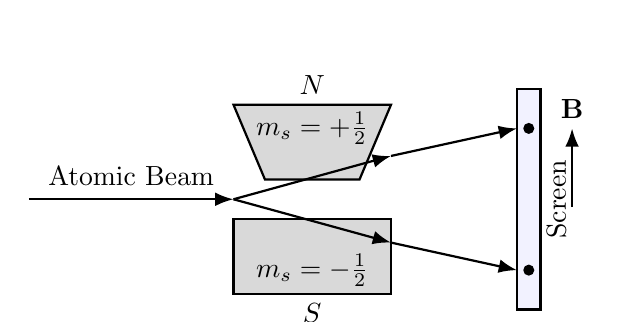
\begin{tikzpicture}[x=1cm,y=1cm,>=Latex,thick]
    % --- Beam (incoming) ---
    \draw[->] (0,0) -- (2.6,0);
    \node at (1.3,0.3) {Atomic Beam};
    
    % --- Stern-Gerlach magnet poles (non-uniform field) ---
    % Top pole: sharp edge
    \draw[fill=gray!30] (2.6,1.2) -- (4.6,1.2) -- (4.2,0.25) -- (3.0,0.25) -- cycle;
    % Bottom pole: flat-ish
    \draw[fill=gray!30] (2.6,-1.2) -- (4.6,-1.2) -- (4.6,-0.25) -- (2.6,-0.25) -- cycle;
    
    \node at (3.6,1.45) {$N$};
    \node at (3.6,-1.45) {$S$};
  % Field direction and gradient note
  \draw[->] (6.9,-0.1) -- (6.9,0.9) node[above] {$\mathbf B$};
    
    % --- Beam splitting inside/out of magnet ---
    \draw[->] (2.6,0) -- (4.6,0.55);
    \draw[->] (2.6,0) -- (4.6,-0.55);
    
    \node[align=center] at (3.6,0.9) {$m_s=+\tfrac12$};
    \node[align=center] at (3.6,-0.9) {$m_s=-\tfrac12$};
    
    % --- Screen / detector ---
    \draw[fill=blue!5] (6.2,-1.4) rectangle (6.5,1.4);
    \node[rotate=90] at (6.7,0) {Screen};
    
    % --- Paths to screen ---
    \draw[->] (4.6,0.55) -- (6.2,0.9);
    \draw[->] (4.6,-0.55) -- (6.2,-0.9);
    
    % --- Spots on screen ---
    \fill (6.35,0.9) circle (2pt);
    \fill (6.35,-0.9) circle (2pt);
    
    \end{tikzpicture}
    \caption{Stern-Gerlach Experiment: An atomic beam of silver atoms is passed through an inhomogeneous magnetic field, resulting in the splitting of the beam into two distinct paths corresponding to spin-up and spin-down states.}
    \label{fig:stern-gerlach}
\end{figure}
Sliver has a spherically symmetric charge distribution plus one 5s-electron. Thus, the total angular momentum of silver is 0, i.e. $l=0$; no splitting should even occur. If the electron from the fifth shell were in a 5p-state, one would then expect a splitting into three beams.
Consequently, the electron must posses a internal angular momentum (spin) with associated magnetic moment, which contributes to the interaction with the magnetic field. The result of the experiment is that the beam is split into two parts, corresponding to two possible orientations of the spin of the electron. This shows that the spin quantum number $m_s$ can take only the values $\pm 1/2$.

\section{Mathematical Description of Spin}
Let the spin operator be $\oS = (\oS_x, \oS_y, \oS_z)$. Now, if $\bfvec{n}$ is a unit vector, we define the spin operator along the direction $\bfvec{n}$ as
\begin{align}
    \oS_n = \bfvec{n} \cdot \oS = n_x \oS_x + n_y \oS_y + n_z \oS_z
\end{align}
As we have done for orbital angular momentum, we postulate that the components of the spin operator satisfy the commutation relations
\begin{align}
    [\oS_i, \oS_j] = \ii \hbar \epsilon_{ijk} \oS_k
\end{align}
where $i,j,k$ run over $x,y,z$. From these commutation relations, we can deduce that the operator $\oS^2 = \oS_x^2 + \oS_y^2 + \oS_z^2$ commutes with each component of $\oS$:
\begin{align}
    [\oS^2, \oS_i] = 0 \quad \text{for } i=x,y,z
\end{align}
Thus, we can find a common set of eigenstates of $\oS^2$ and one component of $\oS$, usually chosen to be $\oS_z$. We denote these eigenstates by $\ket{s,m_s}$, where $s$ is the spin quantum number and $m_s$ is the magnetic spin quantum number. The eigenvalue equations are
\begin{align}
    \oS^2 \ket{s,m_s} & = \hbar^2 s(s+1) \ket{s,m_s} \\
    \oS_z \ket{s,m_s} & = \hbar m_s \ket{s,m_s}
\end{align}
The possible values of $s$ are non-negative integers or half-integers: $s = 0, \frac{1}{2}, 1, \frac{3}{2}, \dots$, and for a given $s$, the possible values of $m_s$ are $m_s = -s, -s+1, \dots, s-1, s$.
\begin{align}
    \oS_+ \ket{s,m_s} & = \hbar \sqrt{s(s+1) - m_s(m_s+1)} \ket{s,m_s+1} \\
    \oS_- \ket{s,m_s} & = \hbar \sqrt{s(s+1) - m_s(m_s-1)} \ket{s,m_s-1}
\end{align}

The state space $\H_t$ of the particle being considered is the tensor product of the spatial part $\H_r$ and the spin part $\H_s$:
\begin{align}
    \H_t = \H_r \otimes \H_s \label{eq:total_space}
\end{align}
Consequently, all spin observables commute with all orbital observables. 



\section{Pauli Matrix}

As we already introduced Spin-1/2 system, we now talk more on the important object: Pauli Matrix. Starting from the commutation relations of the spin operators, 
\begin{align}
    [\oS_i, \oS_j] = \ii \hbar \epsilon_{ijk} \oS_k
\end{align}
which form a Lie algebra $\mathfrak{su}(2)$ of the Lie group $SU(2)$. The dimension of the irreducible representation of this Lie algebra is $2s+1$. For spin-1/2, the dimension is 2, and we can represent the spin operators using $2 \times 2$ matrices. With the eigenvalue equation of $\oS_z$: 
\begin{align}
    \oS_z \ket{s= \tfrac12, m_s = \pm \tfrac12} = \hbar m_s \ket{s= \tfrac12, m_s = \pm \tfrac12}
\end{align}
Choose the orthonormal basis as
\begin{align}
    \upket = \ket{s= \tfrac12, m_s = + \tfrac12} = \begin{pmatrix} 1 \\ 0 \end{pmatrix}, \quad \downket = \ket{s= \tfrac12, m_s = - \tfrac12} = \begin{pmatrix} 0 \\ 1 \end{pmatrix}
\end{align}
Such that 
\begin{align}
    \oS_z \upket = + \frac{\hbar}{2} \upket, \quad \oS_z \downket = - \frac{\hbar}{2} \downket
\end{align}
The matrix representation of $\oS_z$ in this basis is
\begin{align}
    \oS_z = \frac{\hbar}{2} \begin{pmatrix} 1 & 0 \\ 0 & -1 \end{pmatrix}
\end{align}
Look back the raising and lowering operators $\oS_+,\oS_-$, we have
\begin{align}
    \oS_+ \upket & = \hbar \sqrt{\frac12 \left(\frac12 + 1\right) - \frac12 \left(\frac12 + 1\right)} \upket = 0 \\
    \oS_+ \downket & = \hbar \sqrt{\frac12 \left(\frac12 + 1\right) - \left(-\frac12\right) \left(-\frac12 + 1\right)} \upket = \hbar \upket \\
    \oS_- \upket & = \hbar \sqrt{\frac12 \left(\frac12 + 1\right) - \frac12 \left(\frac12 - 1\right)} \downket = \hbar \downket \\
    \oS_- \downket & = \hbar \sqrt{\frac12 \left(\frac12 + 1\right) - \left(-\frac12\right) \left(-\frac12 - 1\right)} \downket = 0
\end{align}
Thus, the matrix representations of $\oS_+$ and $\oS_-$ in this basis are
\begin{align}
    \oS_+ = \hbar \begin{pmatrix} 0 & 1 \\ 0 & 0 \end{pmatrix}, \quad \oS_- = \hbar \begin{pmatrix} 0 & 0 \\ 1 & 0 \end{pmatrix}
\end{align}
From the definitions of $\oS_+$ and $\oS_-$\footnote{$\oS_{\pm} = \oS_x \pm \ii \oS_y$}, we can express
\begin{align}
    \oS_x & = \frac{1}{2} (\oS_+ + \oS_-) = \frac{\hbar}{2} \begin{pmatrix} 0 & 1 \\ 1 & 0 \end{pmatrix} \\
    \oS_y & = \frac{1}{2\ii} (\oS_+ - \oS_-) = \frac{\hbar}{2} \begin{pmatrix} 0 & -\ii \\ \ii & 0 \end{pmatrix}
\end{align}
Now we have the matrix representations of all three spin operators, 
\begin{align}
    \oS_i = \frac{\hbar}{2} \sigma_i, \quad i=x,y,z
\end{align}
where $\sigma_i$ are the Pauli matrices:
\begin{align}
    \sigma_x = \begin{pmatrix} 0 & 1 \\ 1 & 0 \end{pmatrix}, \quad \sigma_y = \begin{pmatrix} 0 & -\ii \\ \ii & 0 \end{pmatrix}, \quad \sigma_z = \begin{pmatrix} 1 & 0 \\ 0 & -1 \end{pmatrix}
\end{align}
And now we can conclude the properties of Pauli Matrices: 
\begin{itemize}
    \item $\sigma_i^2 = I$ for $i=x,y,z$
    \item $\comm{\sigma_i}{\sigma_j} = 2 \ii \epsilon_{ijk} \sigma_k$
    \item $\anticomm{\sigma_i}{\sigma_j} = 2 \delta_{ij} \I_2$
    \item $\Tr{\sigma_i} = 0$
    \item $\det{\sigma_i} = -1$
\end{itemize}

What is more, any $2 \times 2$ Hermitian matrix $M$ can be expressed as a linear combination of the Pauli matrices and the identity matrix:
\begin{align}
    M = a_0 \I_2 + a_x \sigma_x + a_y \sigma_y + a_z \sigma_z
\end{align}
where $a_0, a_x, a_y, a_z$ are real coefficients. This property makes the Pauli matrices a complete basis for the space of $2 \times 2$ Hermitian matrices.

A useful identity involving Pauli matrices is
\begin{align}
    (\bfvec{a} \cdot \boldsymbol{\sigma})(\bfvec{b} \cdot \boldsymbol{\sigma}) = (\bfvec{a} \cdot \bfvec{b}) \I_2 + \ii (\bfvec{a} \times \bfvec{b}) \cdot \boldsymbol{\sigma}
\end{align}

\section{Spinors}
In the basis of $\{\upket, \downket\}$, an arbitrary spin state $\ket{\psi}$ can be represented as a two-component spinor:
\begin{align}
    \ket{\psi} = c_1 \upket + c_2 \downket = \begin{pmatrix} c_1 \\ c_2 \end{pmatrix}
\end{align}
where $c_1$ and $c_2$ are complex coefficients satisfying the normalization condition
\begin{align}
    |c_1|^2 + |c_2|^2 = 1
\end{align}
The general spin state can also be represented by a two-component column vector which is known as a spinor: 
\begin{align}
    \chi = \begin{pmatrix} c_1 \\ c_2 \end{pmatrix}
\end{align}
where 
\begin{align}
    c_1 = \braket{\uparrow|\psi}, \quad c_2 = \braket{\downarrow|\psi}
\end{align}
The basis spinor corresponding to $\upket$ and $\downket$ are
\begin{align}
    \chi_+ = \begin{pmatrix} 1 \\ 0 \end{pmatrix}, \quad \chi_- = \begin{pmatrix} 0 \\ 1 \end{pmatrix}
\end{align}
Thus the general spinor can be written as
\begin{align}
    \chi = c_1 \chi_+ + c_2 \chi_-
\end{align}
The inner product of two spinors $\chi$ and $\phi$ is defined as
\begin{align}
    \braket{\phi|\chi} = \phi^\dag \chi = c_1^* d_1 + c_2^* d_2
\end{align}
where $\phi = \begin{pmatrix} d_1 \\ d_2 \end{pmatrix}$. The norm of a spinor is given by
\begin{align}
    \|\chi\|^2 = \braket{\chi|\chi} = |c_1|^2 + |c_2|^2
\end{align}
The completeness relation in this basis is given by 
\begin{align}
    \upket \upbra + \downket \downbra = \I_2
\end{align}
or in matrix form 
\begin{align}
    \chi_+ \chi_+^\dag + \chi_- \chi_-^\dag = \I_2
\end{align}

\section{Observables and State Vecotrs}
\subsection{State Vectors}
When considering both the spatial and spin degrees of freedom of a particle, the total quantum state is characterized by a ket belonging to the space $\H_t$ which is the tensor product of $\H_r$ and $\H_s$ as \cref{eq:total_space}.
The possible C.S.C.O for such a system is 
\begin{align}
    \{ \hat{\mathbf{r}} , \mathbf{\oS}^2, \oS_z \} \\
    \{ \hat{\mathbf{p}} , \mathbf{\oS}^2, \oS_z \} \\   
    \{ \mathbf{\oL}^2, \oL_z, \mathbf{\oS}^2, \oS_z \}
\end{align}etc.
The common eigenstates of these operators can be denoted as $\ket{\mathbf{r}, \epsilon}$, $\ket{\mathbf{p}, \epsilon}$, or $\ket{n,l,m_l,\epsilon}$ respectively. An example basis of the $\H_t$ can be formed as 
\begin{align}
    \ket{\mathbf{r}, \epsilon} = \ket{\mathbf{r}} \otimes \ket{\epsilon}, \quad \epsilon = \uparrow, \downarrow
\end{align}
By definition, the operators act on these basis states as 
\begin{align*}
    \mathbf{\hat{r}} \ket{\mathbf{r}, \epsilon} & = \mathbf{r} \ket{\mathbf{r}, \epsilon} 
\end{align*}
This operator is exactly $ \mathbf{\hat{r}} = \mathbf{\hat{r}}_r \otimes \oI_s$ where $\mathbf{\hat{r}}_r$ acts on the spatial part $\H_r$ and $\oI_s$ is the identity operator on the spin part $\H_s$. Similarly, the momentum operator is $\mathbf{\hat{p}} = \mathbf{\hat{p}}_r \otimes \oI_s$, and the orbital angular momentum operator is $\mathbf{\oL} = \mathbf{\oL}_r \otimes \oI_s$. The spin operators act only on the spin part: $\mathbf{\oS} = \oI_r \otimes \mathbf{\oS}_s$.
\section{Rotation Group SU(2), SO(3), representations }

\subsection{SU(2) rotation of spin 1/2 system}

Consider a spin 1/2 system, with the operator of spin along an arbitrary direction $\hat{n}$ defined as
\begin{align}
    \hat{S}_n = \vec{\hat{S}} \cdot \hat{n} = \frac{\hbar}{2} \vec{\sigma} \cdot \hat{n}
\end{align}
The eigenvalues of $\hat{S}_n$ are $\pm \hbar/2$, with the corresponding eigenstates denoted as $\upket$ and $\downket$ respectively. Tje rotation operator around the axis $\hat{n}$ by an angle $\theta$ is given by
\begin{align}
    U(\hat{n}, \theta) = e^{-\ii \theta \hat{S}_n / \hbar} = e^{-\ii \frac{\theta}{2} \vec{\sigma} \cdot \hat{n}}
\end{align}
Using the identity for Pauli matrices, we can expand this exponential as
\begin{align}
    U(\hat{n}, \theta) = \cos\left(\frac{\theta}{2}\right) \oI - \ii \sin\left(\frac{\theta}{2}\right) (\vec{\sigma} \cdot \hat{n})
\end{align}





























\chapter{Angular Momentum Addition}

Important for systems with 
\begin{enumerate}
    \item orbital angular momentum $l$ and spin $s$. 
    \item two electron with spin $s_1$ and $s_2$.
    \item two total angular momenta $j_1$ and $j_2$.
\end{enumerate}

\section{Addition of 1/2 Spins}


The mathematical basement of angular momentum addition is the product space as we have disscussed in \cref{sec:product_space}. We consider the two angular momenta $\oJ_1$ and $\oJ_2$ with quantum numbers $j_1$ and $j_2$, magnetic number $m_1$ and $m_2$. 
The total Hilbert space is the tensor product of the Hilbert space of each angular momentum:
\begin{align}
    \H = \H_1 \otimes \H_2
\end{align}
A basis set of $\H$ are $\ket{j_1,m_1}$ and $\ket{j_2,m_2}$, where the two quantum numbers $j_1$ and $j_2$ are fixed, while $m_1$ and $m_2$ vary from $-j_1$ to $j_1$ and from $-j_2$ to $j_2$ respectively. The dimension of the total Hilbert space is
\begin{align}
    \dim{\H} = (2 j_1 + 1)(2 j_2 + 1)
\end{align}
The corresponding basis kets are denoted as
\begin{align}
    \ket{j_1,j_2;m_1,m_2} := \ket{j_1,m_1} \otimes \ket{j_2,m_2}
\end{align}
The total angular momentum operator is given by
\begin{align}
    \mathbf{\oJ}_t = \mathbf{\oJ}_1 \otimes \oI + \oI \otimes \mathbf{\oJ}_2
\end{align}
the components of each angulr momentum satisfy 
\begin{align}
    \comm{\oJ_i}{\oJ_j} = \ii \hbar \epsilon_{ijk} \oJ_k
\end{align}
The eigenvalue equations of $\oJ_1^2$, $\oJ_2^2$, $\oJ_{1z}$ and $\oJ_{2z}$ are\footnote{Here the footnote of $\oI$ does not denote the dimension, but the identity operator in the corresponding Hilbert space.}
\begin{align}
    \mathbf{\oJ}_1^2 \otimes \oI_2 \ket{j_1,j_2;m_1,m_2} & = \mathbf{\oJ}_1^2 \otimes \oI_2 (\ket{j_1,m_1} \otimes \ket{j_2,m_2}) =\hbar^2 j_1 (j_1 + 1) \ket{j_1,j_2;m_1,m_2} \\
    \oI_1 \otimes \mathbf{\oJ}_2^2 \ket{j_1,j_2;m_1,m_2} & = \oI_1 \otimes \mathbf{\oJ}_2^2 (\ket{j_1,m_1} \otimes \ket{j_2,m_2}) =\hbar^2 j_2 (j_2 + 1) \ket{j_1,j_2;m_1,m_2} \\
    \oJ_{1z} \otimes \oI_2 \ket{j_1,j_2;m_1,m_2} & = \oJ_{1z} \otimes \oI_2 (\ket{j_1,m_1} \otimes \ket{j_2,m_2}) = \hbar m_1 \ket{j_1,j_2;m_1,m_2} \\
    \oI_1 \otimes \oJ_{2z} \ket{j_1,j_2;m_1,m_2} & = \oI_1 \otimes \oJ_{2z} (\ket{j_1,m_1} \otimes \ket{j_2,m_2}) =\hbar m_2 \ket{j_1,j_2;m_1,m_2}  
\end{align}
The addition of angular momenta aims to find the eigenkets of the total angular momentum operator $\mathbf{\oJ}_t^2$ and its $z$-component $\oJ_{tz}$:
\begin{align}
    \mathbf{\oJ}_t^2 = (\mathbf{\oJ}_1 \otimes \oI_2 + \oI_1 \otimes \mathbf{\oJ}_2)^2 = \mathbf{\oJ}_1^2 \otimes \oI_2 + \oI_1 \otimes \mathbf{\oJ}_2^2 + 2 (\oJ_{1i} \otimes \oJ_{2i})
\end{align}
As the rasing and lowering operators are $\oJ_{t \pm} = \oJ_{1 \pm} \otimes \oI_2 + \oI_1 \otimes \oJ_{2 \pm}$, and $\oJ_{\pm} = \oJ_x \pm \ii \oJ_y$ 
\begin{align*}
    \mathbf{\oJ}_t^2 & = \mathbf{\oJ}_1^2 \otimes \oI_2 + \oI_1 \otimes \mathbf{\oJ}_2^2 + 2 (\oJ_{1x} \otimes \oJ_{2x} + \oJ_{1y} \otimes \oJ_{2y} + \oJ_{1z} \otimes \oJ_{2z}) \\
    & = \mathbf{\oJ}_1^2 \otimes \oI_2 + \oI_1 \otimes \mathbf{\oJ}_2^2 + (\oJ_{1+} \otimes \oJ_{2-} + \oJ_{1-} \otimes \oJ_{2+}) + 2 (\oJ_{1z} \otimes \oJ_{2z})
\end{align*}
The total angular moemntum operator $\mathbf{\oJ}_t^2$ act on the basis kets $\ket{j_1,m_1} \otimes \ket{j_2,m_2}$ as
\begin{align*}
    \mathbf{\oJ}_t^2 \ket{j_1,m_1} \otimes \ket{j_2,m_2} & = \left[ \hbar^2 j_1 (j_1 + 1) + \hbar^2 j_2 (j_2 + 1) + 2 \hbar^2 m_1 m_2 \right] \ket{j_1,m_1} \otimes \ket{j_2,m_2} \\
    & + \hbar^2 \sqrt{(j_1 - m_1)(j_1 + m_1 + 1)(j_2 + m_2)(j_2 - m_2 + 1)} \ket{j_1,m_1 + 1} \otimes \ket{j_2,m_2 - 1} \\
    & + \hbar^2 \sqrt{(j_1 + m_1)(j_1 - m_1 + 1)(j_2 - m_2)(j_2 + m_2 + 1)} \ket{j_1,m_1 - 1} \otimes \ket{j_2,m_2 + 1}
\end{align*}
We can find that $\mathbf{\oJ}_t^2$ does not have the common eigenkets with $\oJ_{iz}$. We can see this also from the commutation relation\footnote{The convention of $\oJ_{iz}$ here is $\oJ_{1z} \otimes \oI_2$ when $i=1$ and $\oI_1 \otimes \oJ_{2z}$ when $i=2$.}: 
\begin{align*}
    \comm{\mathbf{\oJ}_t^2}{\oJ_{iz}} & = \comm{\mathbf{\oJ}_1^2 \otimes \oI_2 + \oI_1 \otimes \mathbf{\oJ}_2^2 + (\oJ_{1+} \otimes \oJ_{2-} + \oJ_{1-} \otimes \oJ_{2+}) + 2 (\oJ_{1z} \otimes \oJ_{2z})}{\oJ_{iz}} \\
    & = \comm{\oJ_{1+} \otimes \oJ_{2-} + \oJ_{1-} \otimes \oJ_{2+}}{\oJ_{iz}} \ne 0
\end{align*}
The total angular momentum along $z$-direction is given by
\begin{align}
    \oJ_{tz} = \oJ_{1z} \otimes \oI_2 + \oI_1 \otimes \oJ_{2z}
\end{align}
with the eigenvalue equation
\begin{align}
    \oJ_{tz} \ket{j_1,j_2;m_1,m_2} = \hbar (m_1 + m_2) \ket{j_1,j_2;m_1,m_2}
\end{align}
Denoting $m := m_1 + m_2$, we can find in a subspace with fixed $m$, $\mathbf{\oJ}_t^2$ has the common eigenkets with $\oJ_{tz}$. The possible values of $m$ range from $-(j_1 + j_2)$ to $j_1 + j_2$ with step size of $1$. For each fixed $m$, the dimension of the subspace is determined by the number of possible combinations of $m_1$ and $m_2$ satisfying $m = m_1 + m_2$. We can find that the dimension of the subspace is given by
\begin{align}
    \dim{\H_m} = \min(j_1 + j_2 - m, j_1 + j_2 + m) + 1
\end{align}






\chapter{Electromagnetic Field interacting with Quantum Systems}
\section{Charged Harmonic Oscillator in an electromagnetic Field}
The general describtion of a charged particle in an electromagnetic field is given by the Max well equations. Consider a paritcle of mass $m$ and charge $q$ placed in an electromagnetic field assigned with electric field $\bfvec{E}(\bfvec{r},t)$ and the magnetic field $\bfvec{B}(\bfvec{r},t)$. The two fields can satisfy the Max well equations,
\begin{align}
    \nabla \cdot {\bfvec{E}} &= \frac{\rho}{\epsilon_0} \\
    \nabla \cdot{\bfvec{B}} &= 0 \label{eq:charge_nablaB}\\
    \nabla \times{\bfvec{E}} &= - \pdv{\bfvec{B}}{t} \\
    \nabla \times {\bfvec{B}} &= \mu_0 \bfvec{J} + \mu_0 \epsilon_0 \pdv{\bfvec{E}}{t}
\end{align}
Where $\rho(\bfvec{r},t)$ is the charge density, $\bfvec{J}(\bfvec{r},t)$ is the current density, $\epsilon_0$ is the permittivity of free space, and $\mu_0$ is the permeability of free space. The electric and magnetic fields can be expressed in terms of the scalar potential $\phi(\bfvec{r},t)$ and the vector potential $\bfvec{A}(\bfvec{r},t)$ as follows:
\begin{align}
    \bfvec{E}(\bfvec{r},t) &= - \nabla \phi(\bfvec{r},t) - \pdv{\bfvec{A}(\bfvec{r},t)}{t} \label{eq:charge_Efield}\\
    \bfvec{B}(\bfvec{r},t) &= \nabla \times \bfvec{A}(\bfvec{r},t) \label{eq:charge_Bfield}
\end{align}
When we are talking about a given electromagnetic field, we mean exactly a pair of fields $\bfvec{E}(\bfvec r,t)$ and $\bfvec{B}(\bfvec{r},t)$ which can be described by an infinite number of gauges. If we know one gaauge $\{\bfvec{A},\phi \}$, which yields the fields $\bfvec{E}$ and $\bfvec{B}$, then any other gauge $\{\bfvec{A}',\phi'\}$ related to the first by a gauge transformation of the form,
\begin{align}
    \bfvec{A}'(\bfvec{r},t) &= \bfvec{A}(\bfvec{r},t) + \nabla \chi(\bfvec{r},t) \\
    \phi'(\bfvec{r},t) &= \phi(\bfvec{r},t) - \pdv{\chi(\bfvec{r},t)}{t}
\end{align}
where $\chi(\bfvec{r},t)$ is an arbitrary scalar function, will yield the same fields $\bfvec{E}$ and $\bfvec{B}$\footnote{This is an easy proof, it would not be given explicitly here}.

\subsection{Hamiltonian of the System}

In the electromagnetic field, the charaged particle is subject to the Lorentz force, 
\begin{align}
    \bfvec{F} = q \left[ \bfvec{E} + \bfvec{v} \times \bfvec{B} \right]
\end{align}
For a symmetry form, convert the equation above into Gaussian units, we have
\begin{align}
    \bfvec{F} = q \left[ \bfvec{E} + \frac{\bfvec{v}}{c} \times \bfvec{B} \right] \label{eq:Lorentz_force}
\end{align}
For homogeneous fields, the electric and magnetic fields are uniform in space, but may vary with time. Then the homogeneous Maxwell equations in Gaussian units reduce to
\begin{align}
    \nabla \times \bfvec{E} &= - \frac{1}{c} \pdv{\bfvec{B}}{t} \label{eq:charge_GaussianEB}\\
    \nabla \times \bfvec{B} &= \frac{1}{c} \pdv{\bfvec{E}}{t}
\end{align}
Due to \cref{eq:charge_nablaB,eq:charge_Bfield,eq:charge_GaussianEB}, we can ger 
\begin{align}
    \nabla \cdot \left[\bfvec{E} + \frac{1}{c} \pdv{\bfvec{A}}{t} \right] =0
\end{align}
with the scalar potential $\phi$, 
\begin{align}
    \bfvec{E} = - \nabla \phi - \frac{1}{c}\pdv{\bfvec{A}}{t} \label{eq:charge_GaussianEfield}
\end{align}
Pulg this into \cref{eq:Lorentz_force}, we have
\begin{align}
    \bfvec{F} = Q \left[- \nabla \phi - \frac{1}{c} \pdv{\bfvec{A}}{t} + \frac{\bfvec{v}}{c} \times \left( \nabla \times \bfvec{A} \right) \right]
\end{align}
By the identity,
\begin{align}
    \bfvec{v} \times \left( \nabla \times \bfvec{A} \right) = \nabla \left( \bfvec{v} \cdot \bfvec{A} \right) - \left( \bfvec{v} \cdot \nabla \right) \bfvec{A}
\end{align}
The form of the Lorentz force becomes
\begin{align}
    \bfvec{F} = Q \left[- \nabla \phi - \frac{1}{c} \pdv{\bfvec{A}}{t} + \frac{1}{c} \nabla \left( \bfvec{v} \cdot \bfvec{A} \right) - \frac{1}{c} \left( \bfvec{v} \cdot \nabla \right) \bfvec{A} \right]
\end{align}
What is the total time derivative of $\bfvec{A}(\bfvec{r},t)$? By the chain rule, we have
\begin{align}
    \frac{\dd}{\dd t}{\bfvec{A}(\bfvec{r},t)} = \pdv{\bfvec{A}(\bfvec{r},t)}{t} + \left( \bfvec{v} \cdot \nabla \right) \bfvec{A}(\bfvec{r},t)
\end{align}
Plug this into the Lorentz force, we have
\begin{align}
    \bfvec{F} = Q \left[- \nabla \phi + \frac{1}{c} \nabla \left( \bfvec{v} \cdot \bfvec{A} \right) - \frac{1}{c} \frac{\dd \bfvec{A}}{\dd t} \right]
\end{align}
Now we try to find a Lagrangian $L(\bfvec{r},\bfvec{v},t)$, such we can get the Lorentz force from the Lagrangian. Add a vector potential term $U_{\bfvec{A}}(\bfvec{r},\bfvec{v},t) = - Q/c \cdot \bfvec{v} \cdot \bfvec{A}$ to the Lagrangian $L = \frac{1}{2} m \bfvec{v}^2 - Q \phi $, we have 
\begin{align}
    L(\bfvec{r},\bfvec{v},t) = \frac{1}{2} m \bfvec{v}^2 - Q \phi(\bfvec{r},t) + \frac{Q}{c} \bfvec{v} \cdot \bfvec{A}(\bfvec{r},t) \label{eq:lagrangian_em}
\end{align}
By the Euler-Lagrange equation, we have
\begin{align}
    \frac{\dd}{\dd t} \left( \pdv{L}{\bfvec{v}} \right) - \pdv{L}{\bfvec{r}} = 0
\end{align}
Calculate the two terms above, we have
\begin{align}
    \pdv{L}{\bfvec{v}} &= m \bfvec{v} + \frac{Q}{c} \bfvec{A}(\bfvec{r},t) \\
    \pdv{L}{\bfvec{r}} &= - Q \nabla \phi(\bfvec{r},t) + \frac{Q}{c} \bfvec{v} \cdot \nabla \bfvec{A}(\bfvec{r},t)
\end{align}
Then we have
\begin{align}
    \frac{\dd}{\dd t} \left( m \bfvec{v} + \frac{Q}{c} \bfvec{A}(\bfvec{r},t) \right) + Q \nabla \phi(\bfvec{r},t) - \frac{Q}{c} \bfvec{v} \cdot \nabla \bfvec{A}(\bfvec{r},t) = 0
\end{align}
Rearrange this, we have
\begin{align}
    m \frac{\dd \bfvec{v}}{\dd t} = Q \left[- \nabla \phi(\bfvec{r},t) + \frac{1}{c} \nabla \left( \bfvec{v} \cdot \bfvec{A}(\bfvec{r},t) \right) - \frac{1}{c} \frac{\dd \bfvec{A}(\bfvec{r},t)}{\dd t} \right]
\end{align}
The L.H.S is just the Lorentz force \cref{eq:Lorentz_force}. So we have found the Lagrangian of a charged particle in an electromagnetic field. Now we can find the canonical momentum $\bfvec{P}$ conjugate to the coordinate $\bfvec{r}$,
\begin{align}
    \bfvec{P} = \pdv{L}{\bfvec{v}} = \bfvec{p} + \frac{Q}{c} \bfvec{A}(\bfvec{r},t)
\end{align}
The Hamiltonian is given by the Legendre transformation,
\begin{align}
    H = \sum_i p_i v_i - L = \frac{1}{2m} \left( \bfvec{P} - \frac{Q}{c} \bfvec{A}(\bfvec{r},t) \right)^2 + Q \phi(\bfvec{r},t)
\end{align}
Back to the natural units, we have the Hamiltonian of a charged particle in an electromagnetic field,
\begin{align}
    H = \frac{1}{2m} \left( \bfvec{P} - q \bfvec{A}(\bfvec{r},t) \right)^2 + q \phi(\bfvec{r},t)
\end{align}
\subsection{Gauage Transformations}
The gauge fields $\bfvec{A}$ and $\phi$ are not uniquely defined. We can change them as 
\begin{align}
    \phi \ra \phi - \pdv{\alpha}{t} \quad \text{and} \quad \bfvec{A} \ra \bfvec{A} + \nabla \alpha
\end{align}
for any function $\alpha(\bfvec{x},t)$. Under these transformations, the electric and magnetic fields \cref{eq:charge_Efield,eq:charge_Bfield} remain unchanged, as does the Lagrangian \cref{eq:lagrangian_em} in natural units: 
\begin{align*}
    L & \ra \frac{1}{2} m \bfvec{v}^2 - Q (\phi - \pdv{\alpha}{t}) + Q\bfvec{v} \cdot (\bfvec{A} + \nabla \alpha) = L + Q \left( \pdv{\alpha}{t} + \bfvec{v} \cdot \nabla \alpha \right) 
\end{align*}






\subsection{Landau Levels}
we replace the canonical momentum $\bfvec{P}$ by the momentum operator $\op = - \ii \hbar \nabla$, then the Hamiltonian operator becomes
\begin{align}
    \oH = \frac{1}{2m} \left( \op - q \bfvec{A}(\bfvec{r},t) \right)^2 + q \phi(\bfvec{r},t)
\end{align}
Now consider a charged particle moving in a uniform magnetic field $\bfvec{B} = B \hat{z}$, we can choose the vector potential in the Landau gauge,
\begin{align}
    \bfvec{A} = (0, Bx, 0)
\end{align}
and the scalar potential $\phi = 0$. Then the Hamiltonian operator becomes
\begin{align}
    \oH = \frac{1}{2m} \left[ \op_x^2 + \left( \op_y - q B x \right)^2 + \op_z^2 \right]
\end{align}
Since $\H$ commutes with both $\op_y$ and $\op_z$, we can look for simultaneous eigenstates of $\H$, $\op_y$ and $\op_z$. Let these eigenstates be denoted by $\ket{E, k_y, k_z}$, where
\begin{align}
    \oH \ket{E, k_y, k_z} &= E \ket{E, k_y, k_z} \\
    \op_y \ket{E, k_y, k_z} &= \hbar k_y \ket{E, k_y, k_z} \\
    \op_z \ket{E, k_y, k_z} &= \hbar k_z \ket{E, k_y, k_z}
\end{align}
In the position representation, the wavefunction corresponding to the state $\ket{E, k_y, k_z}$ is given by
\begin{align}
    \psi_{E, k_y, k_z}(\bfvec{r}) = \braket{\bfvec{r}|E, k_y, k_z} = \frac{1}{\sqrt{L_y L_z}} \ee^{\ii (k_y y + k_z z)} \phi(x)
\end{align}
where $L_y$ and $L_z$ are normalization lengths in the $y$ and $z$ directions, respectively, and $\phi(x)$ is a function to be determined. Plugging this ansatz into the time-independent Schrödinger equation $\oH \psi_{E, k_y, k_z}(\bfvec{r}) = E \psi_{E, k_y, k_z}(\bfvec{r})$, we obtain an effective one-dimensional Schrödinger equation for $\phi(x)$:
\begin{align}
    \left[ -\frac{\hbar^2}{2m} \frac{\dd^2}{\dd x^2} + \frac{1}{2} m \omega_c^2 \left( x - x_0 \right)^2 \right] \phi(x) = \left( E - \frac{\hbar^2 k_z^2}{2m} \right) \phi(x)
\end{align}
where $\omega_c = \frac{q B}{m}$ is the cyclotron frequency, the eigenvalues of this equation are given by
\begin{align}
    E_{n, k_z} = \hbar \omega_c \left( n + \frac{1}{2} \right) + \frac{\hbar^2 k_z^2}{2m}, \quad n = 0, 1, 2, \ldots
\end{align}
These quantized energy levels $E_{n, k_z}$ are known as Landau levels. The corresponding eigenfunctions $\phi_n(x)$ are given by the harmonic oscillator wavefunctions centered at $x_0 = \frac{\hbar k_y}{q B}$:
\begin{align}
    \phi_n(x) = \left( \frac{m \omega_c}{\pi \hbar} \right)^{1/4} \frac{1}{\sqrt{2^n n!}} \ee^{-\frac{m \omega_c}{2 \hbar} (x - x_0)^2} H_n \left( \sqrt{\frac{m \omega_c}{\hbar}} (x - x_0) \right)
\end{align}
where $H_n$ are the Hermite polynomials. Thus, the complete eigenfunctions of the Hamiltonian in the presence of a uniform magnetic field are given by
\begin{align}
    \psi_{n, k_y, k_z}(\bfvec{r}) = \frac{1}{\sqrt{L_y L_z}} \ee^{\ii (k_y y + k_z z)} \phi_n(x)
\end{align}

\section{Motion in a magnetic field}

We now consider the motion of mass $m$ and charge $e$ in an electromagnetic field. The representation of the field by the vector potential $\bfvec{A}$ and the scalar potential $\Phi$ 
\begin{align*}
    \bfvec{E} & = - \frac{1}{c} \pdv{\bfvec{A}}{t} - \boldsymbol{\nabla} \Phi \\ 
    \bfvec{B} & = \boldsymbol{\nabla} \times \bfvec{A}
\end{align*}

The Hamiltonian of the particle is given by 
\begin{align*}
    H = \frac{1}{2m} \left( \bfvec{p} - \frac{e}{c} \bfvec{A}(\bfvec{x},t) \right)^2 + e \Phi(\bfvec{x},t)
\end{align*}
is known from electrodynamics. Thus the Hamiltonian operator in quantum mechanics is 
\begin{align}
    \oH = \frac{1}{2m} \left( - \ii \hbar \boldsymbol{\nabla} - \frac{e}{c}\bfvec{A} \right)^2 + e \Phi
\end{align}

Expanding the square, we have 
\begin{align*}
    - \frac{\hbar e}{2 \ii m c} \left( \boldsymbol{\nabla}\cdot \bfvec{A} + \bfvec{A} \cdot \boldsymbol{\nabla} \right) \psi = \frac{\ii e \hbar}{m c} \bfvec{A} \cdot \boldsymbol{\nabla} \psi
\end{align*}
where the Coulomb gauge $\boldsymbol{\nabla} \cdot \bfvec{A} = 0$ has been imposed. 
The time-dependent Schrödinger equation is 
\begin{align*}
    \ii \hbar \pdv{\psi}{t} = - \frac{\hbar^2}{2m} \boldsymbol{\nabla}^2 \psi + \frac{\ii \hbar e}{m c} \bfvec{A} \cdot \boldsymbol{\nabla}\psi + \frac{e^2}{2 m c^2} \bfvec{A}^2 \psi + e \Phi \psi
\end{align*}

For a constant magnetic field $\bfvec{B}$, the vector potential can be written as 


\chapter{Arroximation Methods}

\section{Time-independent perturbation theory}
\subsection{Non-degenerate}
Given the Hamiltonian $\oH$, take it as 
\begin{align}
    \oH = \oH_0 + \lambda \oH'
\end{align}
where the Hamiltonian $\oH_0$ is exactly solvable, and $\lambda \oH'$ is a small perturbation. The eigenvalues and eigenstates of $\oH_0$ are known: 
\begin{align}
    \oH_0 \ket{n^0} = E_n^{(0)} \ket{n^0}
\end{align}
which is non-degenerate. We want to find the eigenvalues and eigenstates of $\oH$, using a power series 
\begin{align}
    \ket{n} &= \ket{n^0} + \lambda \ket{n^1} + \lambda^2 \ket{n^2} + \cdots \\
    E_n &= E_n^{(0)} + \lambda E_n^{(1)} + \lambda^2 E_n^{(2)} + \cdots
\end{align}
plugging in this into eigenvalue equation $\oH \ket E = E_n \ket E $
\begin{align}
    &(\oH_0 + \lambda \oH') \left(\ket{n^0} + \lambda \ket{n^1} + \lambda^2 \ket{n^2} + \dots\right) =\\
    & \left(E_n^{(0)} + \lambda E_n^{(1)} + \lambda^2 E_n^{(2)} + \dots\right) \left(\ket{n^0} + \lambda \ket{n^1} + \lambda^2 \ket{n^2} + \dots\right)
\end{align}
compare the coefficients, 
\begin{align}
    & \oH_0 \ket{n^0} = E_n^{(0)} \ket{n^0} \\
    & \oH_0 \ket{n^1} + \oH' \ket{n^0} = E_n^{(0)} \ket{n^1} + E_n^{(1)} \ket{n^0} \label{eq:first_order_perturbation_nonde_tin}\\
    & \oH_0 \ket{n^2} + \oH' \ket{n^1} = E_n^{(0)} \ket{n^2} + E_n^{(1)} \ket{n^1} + E_n^{(2)} \ket{n^0} \label{eq:energyinsecond} \\
    & \cdots \notag
\end{align}
Taking the normalization condition as $\braket{n^0|n} = 1$, i.e. 
\begin{align*}
    \lambda \braket{n^0| n^1} + \lambda^2 \braket{n^0|n^2} + \dots = 0
\end{align*}
whence follows 
\begin{align}
    \braket{n^0 | n^1} = 0, \quad \braket{n^0 | n^2} = 0, \quad \cdots
\end{align}
Consider the unperturbed state $\ket{n^0}$, one can prove that it form a complete orthonormal set, 
\begin{proof}
    \begin{itemize}
        \item Completeness: The unperturbed Hamiltonian $\oH_0$ is self-adjoint, so its eigenkets $\{\ket{n^0}\}$ form a complete set. 
        \item Orthonormality: For $m \neq n$, 
        \begin{align*}
            \braket{m^0|\oH_0|n^0} = E_n^{(0)} \braket{m^0|n^0} \\
            \braket{m^0|\oH_0|n^0} = E_m^{(0)} \braket{m^0|n^0}
        \end{align*}
        since $E_m^{(0)} \neq E_n^{(0)}$, we have $\braket{m^0|n^0} = 0$. As we are considering non-degenerate case, we can always choose the normalization such that $\braket{n^0|n^0} = 1$. Thus the orthonormality is proved.
    \end{itemize}
\end{proof}
Such that we can expand $\ket{n^1}$ in terms of $\{\ket{m^0}\}$,
\begin{align}
    \ket{n^1} = \sum_{m \neq n} c_m \ket{m^0}
\end{align}
with the coefficients $c_m = \braket{m^0|n^1}$. Multiplying \eqref{eq:first_order_perturbation_nonde_tin} by $\bra{m^0}$ from the left, we have 
\begin{align*}
    \bra{m^0} \oH_0 \ket{n^1} + \bra{m^0} \oH' \ket{n^0} = E_n^{(0)} \braket{m^0|n^1} + E_n^{(1)} \braket{m^0|n^0}
\end{align*}
as $\oH_0$ is self-adjoint, $\bra{m^0} \oH_0 = E_m^{(0)} \bra{m^0}$, thus
\begin{align*}
    E_m^{(0)} \braket{m^0|n^1} + \bra{m^0} \oH' \ket{n^0} = E_n^{(0)} \braket{m^0|n^1} + E_n^{(1)} \braket{m^0|n^0}
\end{align*}
Rearrange the terms, we have 
\begin{align}
    \bra{m^0} \oH' \ket{n^0} = (E_n^{(0)} - E_m^{(0)}) \braket{m^0|n^1} = (E_n^{(0)} - E_m^{(0)}) c_m
\end{align}
the first correction to the ket $\ket{n^0}$ is 
\begin{align}
    \ket{n^1} = \sum_{m \neq n} \frac{\bra{m^0} \oH' \ket{n^0}}{E_n^{(0)} - E_m^{(0)}} \ket{m^0}
\end{align}

Multiply \cref{eq:energyinsecond} by $\bra{n^0}$ from the left, we have
\begin{align*}
    &\bra{n^0} \oH_0 \ket{n^2} + \bra{n^0} \oH' \ket{n^1} = E_n^{(0)} \braket{n^0|n^2} + E_n^{(1)} \braket{n^0|n^1} + E_n^{(2)} \braket{n^0|n^0} \\
    \implies &\bra{n^0} \oH_0 \ket{n^2} + \bra{n^0} \oH' \ket{n^1} = E_n^{(2)}
\end{align*}
As $\oH_0$ is self-adjoint, $\bra{n^0} \oH_0 = E_n^{(0)} \bra{n^0}$, thus
\begin{align*}
    E_n^{(0)} \braket{n^0|n^2} + \bra{n^0} \oH' \ket{n^1} = E_n^{(2)}
\end{align*}
Using the normalization condition $\braket{n^0|n^2} = 0$, we have 
\begin{align}
    E_n^{(2)} = \bra{n^0} \oH' \ket{n^1}
\end{align}
plug in the expression of $\ket{n^1}$, we have
\begin{align}
    E_n^{(2)} = \sum_{m \neq n} \frac{|\bra{n^0} \oH' \ket{m^0}|^2}{E_n^{(0)} - E_m^{(0)}}
\end{align}
\subsection{Degenerate}





\section{Variational method}

\section{WKB approximation}

\section{Time-dependent perturbation theory}

Consider a stationary physical system with $\oH_0$ which is exactly solvable, i.e., the eigenvalues and eigenvectors are known: 
\begin{align}
    \oH_0 \ket{n} = E_n \ket{n}
\end{align}
For simplicity, assume the spectrum is non-degenerate and discrete. At some time $\tau_s$, a perturbation is switched on, 
\begin{align}
    \oH(t) = \oH_0 + \lambda \hat{V} (t)
\end{align}
with $\hat{V}(t)$ being an observables which is dependent on time, and $\lambda$ is a small parameter. The system is initially in the stationary state $\ket{i}$, an eigenstate of $\oH_0$ with eigenvalue $E_i$. After the perturbation is applied, the system evolves: the state $\ket{i}$ is no longer an eigenstate of the perturbation Hamiltonian. The object of time-dependent perturbation theory is to calculate the probability of finding the system in a certain state $\ket{f}$ at time $t > \tau_s$. In other words, we want to study the transitions that can be introduced by the perturbation between the stationary states of the unperturbed system.

Before the time $\tau_s$, the system is in the state $\ket{i}$, satisfying 
\begin{align}
    \ii \hbar \pdv{}{t} \ket{i(t)} = \oH_0 \ket{i(t)}
\end{align}
after the time $\tau_s$, the system evolves according to
\begin{align}
    \ii \hbar \pdv{}{t} \ket{\psi(t)} = \left(\oH_0 + \lambda \hat{V}(t)\right) \ket{\psi(t)} \label{eq:time_perturbation_seq}
\end{align}
with initial condition 
\begin{align}
    \ket{\psi(\tau_s)} = \ket{i}
\end{align}
The desired probability can be calculated as \footnote{Later the arrow inside the script of P will be neglected for simplicity, this just indicates that this probability is the transition from initial state to final state.}
\begin{align}
    P_{i \to f} (t) = \abs{\braket{f|\psi(t)}}^2
\end{align}
We find now the operators and states are both time-dependent, such that it is necessary to choose a representation to deal with this problem. Here we choose the interaction picture. In the interaction picture, the states and operators are defined as
\begin{align}
    \ket{\psi(t)}_I &= \ee^{\frac{\ii}{\hbar} \oH_0 t} \ket{\psi(t)} \\
    \oA_I (t) &= \ee^{\frac{\ii}{\hbar} \oH_0 t} \oA(t) \ee^{-\frac{\ii}{\hbar} \oH_0 t}
\end{align}
recall \cref{eq:time_perturbation_seq}, differentiate the ket in interaction picture: 
\begin{align}
    &\ii \hbar \pdv{}{t} \ket{\psi(t)}_I = - \oH_0 \ket{\psi(t)}_I + \ee^{\ii \oH_0 t/\hbar} \left[\oH_0 + \lambda \oV(t)\right] \ket{\psi(t)} \\
    \implies & \ii \hbar \pdv{}{t} \ket{\psi(t)}_I = \lambda \oV_I(t) \ket{\psi(t)}_I \label{eq:schrodinger_interaction_picture}
\end{align}
Integrating \cref{eq:schrodinger_interaction_picture} over time: 
\begin{align}
    \ket{\psi(t)}_I = \ket{\psi(t_0)}_I - \frac{\ii}{\hbar}\lambda \int_{\tau_s}^{t} \dd t' \oV_I(t') \ket{\psi(t')}_I
\end{align}
Iteraing this equation, from the initial condition $\ket{\psi(\tau_s)}_I = \ket{i}$, we have 
\begin{itemize}
    \item the 0-th order approximation: 
\begin{align}
    \ket{\psi(t)}_I^{(0)} = \ket{i}
\end{align}
    \item the 1-st order approximation:
    \begin{align}
        \ket{\psi(t)}_I^{(1)} = \ket{i} - \frac{\ii}{\hbar} \lambda\int_{\tau_s}^{t} \dd t' \oV_I(t') \ket{i} \label{eq:first_order_timeper}
    \end{align}
    \item the 2-nd order approximation:
    \begin{align}
        \ket{\psi(t)}_I^{(2)} = \ket{i} - \frac{\ii}{\hbar} \lambda \int_{\tau_s}^{t} \dd t' \oV_I(t') \left( \ket i - \frac{\ii}{\hbar} \lambda \int_{\tau_s}^{t'} \dd t'' \oV_I(t'') \ket{i} \right)
    \end{align}
    \item \dots 
\end{itemize}
This expansion was so called Neumann series. In principle, it allows one to calculate the state up to arbitrary order in the perturbation.

\subsection{First-Order Perturbation}

Let the system is initially in the eigenstate
\begin{align}
    \ket{i(t)} = \ee^{- \ii \oH_0 t/\hbar} \ket{i} = \ee^{-\ii E_i t/\hbar} \ket{i}
\end{align}
of the unperturbed Hamiltonian $\oH_0$. What is the probability of finding the system at the time $t$ in the state 
\begin{align}
    \ket{f(t)} = \ee^{-\ii \oH_0 t/\hbar} \ket{f} = \ee^{-\ii E_f t/\hbar} \ket{f}
\end{align}
after the action of $\oV(t)$? First it is easy to find the probability amplitude: 
\begin{align}
    \braket{f(t)|\psi(t)} = \bra{f} \ee^{\ii \oH_0 t/\hbar} \ket{\psi(t)} = \braket{f|\psi(t)}_I
\end{align}
The initial state is $\ket{i}$, the probability amplitude of first order approximation \cref{eq:first_order_timeper} is 
\begin{align}
    \braket{f(t)|\psi(t)} &= \delta_{f,i} - \frac{\ii \lambda}{\hbar} \int_{\tau_s}^{t} \dd t' \bra{f} \oV_I(t') \ket{i} \notag \\
    &= \delta_{f,i} - \frac{\ii \lambda}{\hbar} \int_{\tau_s}^{t} \dd t' \bra{f} \ee^{\ii \oH_0 t' /\hbar} \oV(t') \ee^{- \ii \oH_0 t'/ \hbar} \ket{i} \notag \\ 
    &= \delta_{f,i} - \frac{\ii \lambda}{\hbar} \int_{\tau_s}^{t} \dd t' \ee^{\ii (E_f - E_i) t'/ \hbar} \bra{f} \oV(t') \ket{i}.
\end{align}
The transition probability $P_{if}$ for the transition of $\ket i$ to another orthogonal state $\ket f$ is the square of the modulus of this expression: 
\begin{align}
    P_{if} (t) = \abs{\braket{f(t)|\psi(t)}}^2 = \abs{\frac{\lambda}{\hbar} \int_{\tau_s}^{t} \dd t' \ee^{\ii(E_f-E_i)t'/\hbar} \bra{n} \oV(t') \ket{i} }^2 \label{eq:timedependent_transition_probability}
\end{align}
\subsection{Transitions into a Continuous Spectrum, and the Fermi Golden Rule}
Now apply the probability we obtained in the previous section into a continuous spectrum of final states. There are several examples of this case: 
\begin{enumerate}
    \item Scattering: Here, the momentum $\bfvec{ k}$ of a particle goes over $\bfvec{k}'$. 1-st order perturbation theory leads to the Born approximation of scattering theory.
    \item $\alpha-$Decay: Here as well, the final states, i.e., the momenta of the $\alpha$ particles, lie in a continuum.
    \item Optical transitions: An excited state makes a transition to a lower state by emitting a photon, whose momentum varies continuously.
\end{enumerate}
Consider a perturbation that is swithced on at time $t=0$ and subquently remains unchanged: 
\begin{align}
    \oV(t) = \oV \Theta(t)
\end{align}
substituting this back into \cref{eq:timedependent_transition_probability}, we have
\begin{align}
    P_{if} (t) = \frac{1}{\hbar^2} \abs{\int_{0}^{t} \dd t' \ee^{}}
\end{align}





\section{Adiabatic Approximation}

\subsection{Adiabatic Theorem}

\begin{definition}[Adiabatic Process]
    The Hamiltonian $\oH(t)$ of a quantum system changes gradually, such that the system can adopt its configuration to the changed Hamiltonian. If the system starts in an eigenstates of the original Hamiltonian, it will end in the corresponding eigenstate of the final Hamiltonian.
\end{definition}

For a time independent Hamiltonian $\oH$, the time-dependent Schrödinger equation has a solution of the form
\begin{align}
    \ket{\Psi_n(t)} = \ee^{-\ii E_n t/\hbar} \ket{n}, \text{ with }, \oH \ket{\Psi_n} = E_n \ket{\Psi_n}
\end{align}
The general solution is 
\begin{align}
    \ket{\Psi_n(t)} = \sum_n c_n \ee^{-\ii E_n t/\hbar} \ket{n}, \text{ with } c_n = \braket{n|\Psi(0)}
\end{align}
A time-dependent Hamiltonian $\oH(t)$ has at every instance of time eigenfunctions and eigenvalues
\begin{align}
    \oH(t) \ket{n(t)} = E_n(t) \ket{n(t)}
\end{align}
with $\sum_n \ket{n(t)}\bra{n(t)} = \oI$, and $\braket{n(t)|n(t')} = \delta_{t t'}$. Note that $\ket{n(t)}$ are not the solution of the time-dependent Schrödinger equation, but they are the instantaneous eigenstates of the Hamiltonian at time $t$. The adiabatic theorem states that if the Hamiltonian changes slowly enough, then a system initially in an eigenstate of $\oH(0)$ will remain in the corresponding instantaneous eigenstate of $\oH(t)$ at later times, up to a phase factor. 
\begin{align}
    \ket{n(t)} = \sum_n c_n(t) \ee^{-\ii \theta_n(t)} \ket{n(t)}
\end{align}
with the phase 
\begin{align}
    \theta_n(t) = \frac{1}{\hbar} \int_0^t E_n(t') \dd t'
\end{align}
Substituting this into the time-dependent Schrödinger equation, we have
\begin{align*}
    \ii \hbar \pp_t \left( \sum_n c_n(t) \ee^{-\ii \theta_n(t)} \ket{n(t)} \right) = \oH(t) \sum_n c_n(t) \ee^{-\ii \theta_n(t)} \ket{n(t)}\\
    \ii \hbar \sum_n \left[ \dot c_n \ket{n(t)} + c_n \dot{\ket{n(t)}} - \ii c_n \dot{\theta_n} \ket{n(t)} \right] \ee^{- \ii \theta_n(t)} =\sum_n c_n E_n(t) \ket{n(t)}
\end{align*}
with $\dot \theta_n = E_n(t)/\hbar$, we have 
\begin{align}
    \sum_n \dot c_n \ket{n(t)} \ee^{-\ii \theta_n(t)} = - \sum_n c_n \dot{\ket{n(t)}} \ee^{-\ii \theta_n(t)} 
\end{align}
We can not get the coefficients $c_n$ from this equation, but we can get the transition probability between different instantaneous eigenstates. Multiplying $\bra{m(t)}$ from the left, we have





\chapter{Symmetry in Quanbtum Mechanics} \label{chap:Symmetry}

What we mean by symmetry in Quantum Mechanics is similar to that in Classical Physics. A symmetry transformation is represented by a unitary (or anti-unitary) operator $\oU$ that acts on the state vectors in the Hilbert space. If the Hamiltonian $\oH$ of a system commutes with the symmetry operator $\oU$, i.e., $\comm{\oH}{\oU}=0$, then the system is said to possess that symmetry. This implies that the physical properties of the system remain unchanged under the transformation represented by $\oU$.

\section{Continuous Symmetry}
\subsection{Translation Symmetry} \label{sec:translation_symmetry}

Consider a Hilbert space $\H$ and a vector $\kps \in \H$, the wave function in the position representation is given by $\psi(\bfvec{r}) = \braket{\bfvec{r}|\psi}$. One can define a translation in space by a vector $\bfvec{a}$ as follows:
\begin{align}
    \bfvec{r} \rightarrow \bfvec{r}' = \bfvec{r} + \bfvec{a}
\end{align}

The spatial vector $\bfvec{a}$ is a constant vector. If the physics is invariant under such spcae translations, then we say the system has translation symmetry. The wave function naively follows: 
\begin{align}
    \psi'(\bfvec{r}') \equiv \psi(\bfvec{r}) \label{eq:translation_wavefunction}
\end{align}
such that 
\begin{align}
    \psi'(\bfvec{r} + \bfvec{a}) = \psi(\bfvec{r}) \quad \text{or} \quad \psi'(\bfvec{r}) = \psi(\bfvec{r} - \bfvec{a}) 
\end{align}

Define a spatial translation operator $\oT(\bfvec{a})$, such that \cref{eq:translation_wavefunction} can be written as
\begin{align}
    \psi'(\bfvec{r}) = \oT(\bfvec{a}) \psi (\bfvec{r})
\end{align}

The probability must be invariant under such translation, i.e.,
\begin{align}
    \braket{\psi'|\psi'} &= \int \dd^3 \bfvec{r} \braket{\psi'|\bfvec{r}} \braket{\bfvec{r}|\psi'} = \int \dd^3 \bfvec{r} {\psi'}^*(\bfvec{r}) \psi'(\bfvec{r}) = \int \dd^3 \bfvec{r} \left[\oT(\bfvec{a}) \psi(\bfvec{r})\right]^* \oT(\bfvec{a}) \psi(\bfvec{r}) \\
    &= \int \dd^3 \bfvec{r} \psi^*(\bfvec{r}) \oT^ \dag(\bfvec{a}) \oT(\bfvec{a}) \psi(\bfvec{r}) = \int \dd^3 \bfvec{r} \psi^*(\bfvec r) \psi(\bfvec r) = \braket{\psi|\psi} \label{eq:translation_probability}
\end{align}
from \cref{eq:translation_probability}, we can see that the translation operator $\oT(\bfvec{a})$ must be unitary: 
\begin{align}
    \oT^ \dag(\bfvec{a}) \oT(\bfvec{a}) = \I \quad \Longleftrightarrow \quad \oT^ \dag (\bfvec{a}) = \oT^{-1}(\bfvec{a})
\end{align}
Now we explicitly find the form of the translation operator. Consider an unit translation $\bfvec{a}$, we can expand the wave function $\psi(\bfvec{r} - \bfvec{a})$ in Taylor series:
\begin{align*}
    \psi(\bfvec{r} - \bfvec{a}) &= \psi(\bfvec{r}) - \bfvec{a} \cdot \nabla \psi(\bfvec{r}) + \frac{1}{2!} (\bfvec{a} \cdot \nabla)^2 \psi(\bfvec{r}) - \frac{1}{3!} (\bfvec{a} \cdot \nabla)^3 \psi(\bfvec{r}) + \dots   \\
    &= \exp(-\bfvec{a} \cdot \nabla) \psi(\bfvec{r}) = \exp \left(- \frac{\ii \bfvec{a} \cdot \op}{\hbar}\right) \psi(\bfvec{r}) \numberthis \label{eq:translation_operator_form}
\end{align*}
where the momentum operator in the position representation is given by $\op = - \ii \hbar \nabla$. Comparing \cref{eq:translation_operator_form} with the definition of translation operator, we find that the translation operator can be expressed as
\begin{align}
    \oT(\bfvec{a}) = \exp \left(- \frac{\ii \bfvec{a} \cdot \op}{\hbar}\right)
\end{align}

Now we can consider a different approach to derive the translation operator. Consider an infinitesimal translation $\delta \bfvec{a} = \bfvec{\epsilon}$, for arbirtay wave function $\psi(\bfvec{r})$, the translated wave function is given by
\begin{align}
    (\oT(\bfvec{\epsilon})\psi)(\bfvec{r}) = \psi(\bfvec{r}-\bfvec{\epsilon}).
\end{align}
expanding the r.h.s in Taylor series, we have
\begin{align}
    \psi(\bfvec{r}-\bfvec{\epsilon}) = \psi(\bfvec{r}) - \bfvec{\epsilon} \cdot \nabla \psi(\bfvec{r}) + \O(\epsilon^2) 
\end{align}
Such that we can find the translation operator for infinitesimal translation is given by
\begin{align}
    \oT(\bfvec{\epsilon}) = \I - \bfvec{\epsilon} \cdot \nabla + \O(\epsilon^2)
\end{align}
Due to \cref{sec:GroupRepresentations}, the unitay representation of a continuous group can always be expressed as 
\begin{align}
    \oT(\epsilon) =\oI + \epsilon \oG + \O(\epsilon^2)
\end{align}
The hermitian conjugate of the translation operator is 
\begin{align}
    \oT^ \dag(\bfvec{\epsilon}) = \I + \bfvec{\epsilon} \oG^ \dag+ \O(\epsilon^2)
\end{align}
The unitarity condition requires that
\begin{align}
    \oT^ \dag(\bfvec{\epsilon}) \oT(\bfvec{\epsilon}) = \I + \bfvec{\epsilon} (\oG^ \dag + \oG) + \O(\epsilon^2) = \I
\end{align}
which implies that the generator $\oG$ is anti-hermitian, i.e., $\oG^ \dag = - \oG$. Comparing with the previous result, we find that the generator of translation is given by\footnote{$\hbar$ is introduced to make the generator have the dimension of momentum.}
\begin{align}
    \oG = - \nabla = \frac{\ii}{\hbar} \op
\end{align}
Thus the translation operator for finite translation $\bfvec{a}$ can be expressed as
\begin{align}
    \oT(\bfvec{a}) = \exp \left(- \frac{\ii \bfvec{a} \cdot \op}{\hbar}\right)
\end{align}
\newpage
\subsection{Rotation Symmetry}
Consider a rotation in 3D space $R$, which acts on a position vector $\bfvec{r}$ as
\begin{align}
    \bfvec{r} \rightarrow \bfvec{r}' = R \bfvec{r}
\end{align}
Usually, we denote the rotation forms a group $SO(3)$, which is disscussed in Appendix.\ref{chap:GroupTheory}. Consider a rotation about a fixed axis, e.g. the $z$-axis by an angle $\delta \theta$, also denoting $\delta \vec{\theta}$ to be a vector of magnitude $\delta \theta$ and direction along the axis of rotation. Using these we can rewirte the rotation as 
\begin{align}
    \bfvec{r} \ra \bfvec{r}' = \bfvec{r} + \delta \vec{\theta} \times \bfvec{r}
\end{align}
The change of position vector is $\delta \bfvec{r} = \delta \vec{\theta} \times \bfvec{r}$. Similarly, the momentum vector would change as $\delta \bfvec{p} = \delta \vec{\theta} \times \bfvec{p}$. A rotation symmetry implies that the physics is invariant under such rotation, i.e., for an arbitrary wave function $\psi(\bfvec{r})$, the rotated wave function is given by
\begin{align}
    \psi'(\bfvec{r}) = \psi (\bfvec{r}') = \psi \left(\bfvec{r}+ \delta \vec{\theta} \times \bfvec{r}\right)
\end{align}
Define a rotation operator $\oR(\delta \vec{\theta})$, such that
\begin{align}
    \psi'(\bfvec{r}) = \oR(\delta \vec{\theta}) \psi(\bfvec{r})
\end{align}
The probability must be invariant under such rotation, i.e.,
\begin{align}
    \braket{\psi'|\psi'} &= \int \dd^3 \bfvec{r} \braket{\psi'|\bfvec{r}} \braket{\bfvec{r}|\psi'} = \int \dd^3 \bfvec{r} {\psi'}^*(\bfvec{r}) \psi'(\bfvec{r}) = \int \dd^3 \bfvec{r} \left[\oR(\delta \vec{\theta}) \psi(\bfvec{r})\right]^* \oR(\delta \vec{\theta}) \psi(\bfvec{r}) \\
    &= \int \dd^3 \bfvec{r} \psi^*(\bfvec{r}) \oR^ \dag(\delta \vec{\theta}) \oR(\delta \vec{\theta}) \psi(\bfvec{r}) = \int \dd^3 \bfvec{r} \psi^*(\bfvec r) \psi(\bfvec r) = \braket{\psi|\psi} 
\end{align}
From the equation above, we can see that the rotation operator $\oR(\delta \vec{\theta})$ must be unitary: 
\begin{align}
    \oR^ \dag(\delta \vec{\theta}) \oR(\delta \vec{\theta}) = \I \quad \Longleftrightarrow \quad \oR^ \dag (\delta \vec{\theta}) = \oR^{-1}(\delta \vec{\theta})
\end{align}
Now we explicitly find the form of the rotation operator. Consider an infinitesimal rotarion $\delta \vec{\theta}$, we can expand the wave function $\psi(\bfvec{r} + \delta \vec{\theta} \times \bfvec{r})$ in Taylor series:
\begin{align*}
    \psi(\bfvec{r} + \delta \vec{\theta} \times \bfvec{r}) &= \psi(\bfvec{r}) + (\delta \vec{\theta} \times \bfvec{r}) \cdot \nabla \psi(\bfvec{r}) + \frac{1}{2!} \left[(\delta \vec{\theta} \times \bfvec{r}) \cdot \nabla\right]^2 \psi(\bfvec{r}) + \dots   \\
    &= \exp\left[(\delta \vec{\theta} \times \bfvec{r}) \cdot \nabla\right] \psi(\bfvec{r}) = \exp\left(- \frac{\ii}{\hbar} \delta \vec{\theta} \cdot \boL\right) \psi(\bfvec{r}) \numberthis \label{eq:rotation_operator_form}
\end{align*}
where thr angular momentum operator in the position representation is given by $\boL = - \ii \hbar \hat{r} \times \nabla =  \hat{r} \times \op $. Comparing \cref{eq:rotation_operator_form} with the definition of rotation operator, we find that the rotation operator can be expressed as
\begin{align}
    \oR(\delta \vec{\theta}) = \exp\left(- \frac{\ii}{\hbar} \delta \vec{\theta} \cdot \boL\right) 
\end{align}
Now we can consider a similar approach of group representation as in the translation symmetry to derive the rotation operator. Consider an infinitesimal rotation $\delta \vec{\theta}$, for arbirtay wave function $\psi(\bfvec{r})$, the rotated wave function is given by
\begin{align}
    (\oR(\delta \vec{\theta})\psi)(\bfvec{r}) = \psi(\bfvec{r} + \delta \vec{\theta} \times \bfvec{r}).
\end{align}
Expanding the r.h.s in Taylor series, we have
\begin{align}
    \psi(\bfvec{r} + \delta \vec{\theta} \times \bfvec{r}) = \psi(\bfvec{r}) + (\delta \vec{\theta} \times \bfvec{r}) \cdot \nabla \psi(\bfvec{r}) + \O(\delta \theta^2) 
\end{align}
Such that we can find the rotation operator for infinitesimal rotation is given by
\begin{align}
    \oR(\delta \vec{\theta}) = \I + (\delta \vec{\theta} \times \bfvec{r}) \cdot \nabla + \O(\delta \theta^2)
\end{align}
Due to Appendix.\ref{sec:GroupRepresentations}, the unitay representation of a continuous group can always be expressed as 
\begin{align}
    \oR(\delta \vec{\theta}) =\oI + \delta \vec{\theta} \cdot \oG + \O(\delta \theta^2)
\end{align}
The hermitian conjugate of the rotation operator is 
\begin{align}
    \oR^ \dag(\delta \vec{\theta}) = \I + \delta \vec{\theta} \cdot \oG^ \dag+ \O(\delta \theta^2)
\end{align}
The unitarity condition requires that
\begin{align}
    \oR^ \dag(\delta \vec{\theta}) \oR(\delta \vec{\theta}) = \I + \delta \vec{\theta} \cdot (\oG^ \dag + \oG) + \O(\delta \theta^2) = \I
\end{align}
which implies that the generator $\oG$ is anti-hermitian, i.e., $\oG^ \dag = - \oG$. Comparing with the previous result, we find that the generator of rotation is given by\footnote{$\hbar$ is introduced to make the generator have the dimension of angular momentum.}
\begin{align}
    \oG = - \left(\bfvec{r} \times \nabla \right) = \frac{\ii}{\hbar} \boL
\end{align}
Thus the rotation operator for finite rotation $\vec{\theta}$ can be expressed as
\begin{align}
    \oR(\vec{\theta}) = \exp\left(- \frac{\ii}{\hbar} \vec{\theta} \cdot \boL\right)    
\end{align}

\subsection{Internal continuous Symmetry: Gauge invariance}
We consider first a global (r,t independent) phase transformation of a wave function, a $U(1)$ gauge transformation, 
\begin{align}
    U = \ee^{- \ii \phi} \quad \Longrightarrow \quad \psi(\bfvec{r},t) \ra \psi'(\bfvec{r},t) = U \psi(\bfvec{r},t) = \ee^{- \ii \phi} \psi(\bfvec{r},t)
\end{align}
The Hamiltonian is invariant under such transformation, i.e., $\oH' = U \oH U^ \dag = \oH$\footnote{As the phase factor is independent of $r,t$, $\comm{\phi \oG_ \phi}{\oH} = 0$}. The generator of the phase transformation is in this representation obviouly $\oG_ \phi = \I$. Hence we have the conserved quantity 
\begin{align}
    0 = \ddx{t} \bra{\psi} \oG_ \phi \ket{\psi} = \ddx{t} \braket{\psi|\psi} = \ddx{t} \int \dd^3 x \psi^* \psi =\ddx{t} N
\end{align}
where $N$ is the total probability (or total number of particles in second quantization). Thus the global phase symmetry leads to the conservation of total probability (or total number of particles).

\subsubsection{Local U(1) gauge symmetry}
We postulate that the Schrödinger equation shall be form invariant under $U(1)$ gauge transformations (Yang-Mills). 
\begin{align*}
    \psi'(\bfvec{r},t) = \ee^{- \ii \alpha(\bfvec{r},t)} \psi(\bfvec{r},t)
\end{align*}
\subsection{Symmetry and Conservation Laws}

As we have disscussed in \cref{sec:time_evolution_operator}, 

\newpage
\section{Discrete Symmetry: Parity, Lattice Translation, Time Reversal}
\subsection{Parity Symmetry}
We have discussed what is a parity operaotr in \cref{sec:parity_operator}. 

The wave function in a rotationally invariant potential have the following form:
\begin{align*}
    \braket{x|n,l,m} = R_n(r) Y_l^m(\theta, \phi)
\end{align*}
The transformation $x \mapsto -x$ in spherical coordinates is equivalent to the following: 
\begin{align*}
    r \mapsto r,\quad \theta \mapsto \pi - \theta ,\quad\phi \mapsto \phi + \pi
\end{align*}
means 
\begin{align*}
    \cos \theta \mapsto - \cos \theta, \quad \sin \theta \mapsto \sin \theta, \quad \ee^{\ii m \phi} (-1)^m \ee^{\ii m \phi}
\end{align*}
\subsection{Symmetrical double well potential}
Consider a symmetrical double well potential $V(x)$, such that $V(x) = V(-x)$. Give the potential in an explicit form:
\begin{align}
    V(x) =\begin{cases}
        \infty, & \abs x > a+b, \\
        V_0, &  \abs x < a,\\
        0, & a < \abs{a} < a+b \\
    \end{cases}
\end{align}
The shcematic representation of the potential is shown below:
\begin{figure}[!h]
    \centering
    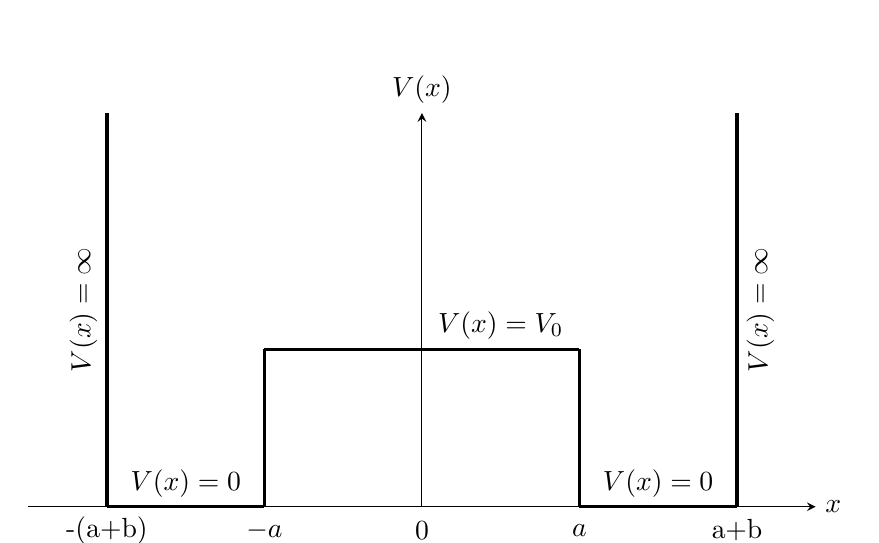
\begin{tikzpicture}[>=stealth, scale=1]
        \draw[->] (-5,0) -- (5,0) node[right] {$x$};
        \draw[->] (0,0) -- (0,5) node[above] {$V(x)$};
        \draw[very thick] (-2,2) -- (2,2);  
        \draw[very thick] (-2,0) -- (-2,2);      
        \draw[very thick] (2,0) -- (2,2);      
        \draw[very thick] (2,0) -- (4,0);
        \draw[very thick] (-4,0) -- (-2,0);
        \draw[very thick] (4,0) -- (4,5); 
        \draw[very thick] (-4,0) -- (-4,5);
        \node[rotate=90] at (-4.3,2.5) {$V(x)=\infty$};
        \node[rotate=90] at (4.3,2.5) {$V(x)=\infty$};
        \node at (0, -0.3) {0};
        \node at (2, -0.3) {$a$};
        \node at (-2, -0.3) {$-a$};
        \node at (3,0.3) {$V(x)=0$};
        \node at (-3,0.3) {$V(x)=0$};
        \node at (4,-0.3) {a+b};
        \node at (-4,-0.3) {-(a+b)};
        \node at (1,2.3) {$V(x)=V_0$};
    \end{tikzpicture}
\end{figure}

Since the potential is symmetric, the Hamiltonian $\oH$ commutes with the parity operator $\oPi$, i.e., $\comm{\oH}{\oPi} = 0$ \footnote{As we have disscussed in \cref{sec:parity_operator}}. Thus the energy eigenstates can be chosen to be simultaneous eigenstates of both $\oH$ and $\oPi$. The parity operator has eigenvalues $\pm 1$, corresponding to even and odd parity states, respectively. Therefore, the energy eigenstates can be classified into two categories: even parity states $\ket S$ (symmetric) and odd parity states $\ket A$ (antisymmetric).

By solving the time-independent Schrödinger equation for different regions, 
\begin{align}
    &- \frac{\hbar^2}{2m} \frac{\dd^2 \psi_1(x)}{\dd x^2}  = E_1 \psi_1(x) \quad a<\abs{x}<a+b\\
    &- \frac{\hbar^2}{2m} \frac{\dd^2 \psi_2(x)}{\dd x^2} + V_0 \psi_2(x) = E_2 \psi_2(x) \quad  \abs{x} < a 
\end{align}
here we can set $k = \sqrt{2mE}/\hbar$ and $\kappa = \sqrt{2m(E-V_0)}/\hbar $the area for $V(x) = \infty$ is infinite, thus the wave function must vanish in that region, i.e. at the coundary $\psi(a+b) = \psi(-(a+b)) = 0$. Actually we can just write one side since the wave function is either even or odd. The solutions are 
\begin{align}
    \psi_1(x) &= \begin{cases}
        A \cos(k x), & \text{even parity} \\
        C \sin(k x), & \text{odd parity} \\
\end{cases} \quad a< \abs{x} < a+b \\
    \psi_2(x) &= \begin{cases}
        B \cosh(\kappa x), & \text{even parity} \\
        D \sinh(\kappa x), & \text{odd parity} \\
    \end{cases} \quad \abs{x} < a
\end{align}
By the boundary condition mentioned above, we can obtain a general case for $\psi_1$
\begin{align}
    \psi_1(x) = \begin{cases}
        A \cos\left[k(x - a - b)\right], & \text{even parity} \\
        C \sin\left[k(x - a - b)\right], & \text{odd parity} \\
\end{cases} 
\end{align}
we disscuss the two cases separately.
\begin{itemize}
    \item \emph{Even parity}: The boundary condition of such case is $\psi_1(a)= \psi_2(a)$ and $\psi_1'(a) = \psi_2'(a)$. Applying these boundary conditions, we have
    \begin{align*}
        A \cos(kb) &= B \cosh(\kappa a) \\
        Ak \sin(kb) & = B \kappa \sinh(\kappa a)
    \end{align*}
    From these two, we can eliminate $A$ and $B$, obtaining the transcendental equation for even parity states:
    \begin{align}
        k \tan(kb) = \kappa \tanh(\kappa a) \label{eq:SDWP_quant1}
    \end{align}
    \item \emph{Odd parity}: The boundary condition of such case is $\psi_1(a)= \psi_2(a)$ and $\psi_1'(a) = \psi_2'(a)$. Applying these boundary conditions, we have
    \begin{align*}
        C \sin(kb) &= D \sinh(\kappa a) \\
        Ck \cos(kb) & = D \kappa \cosh(\kappa a)
    \end{align*}
    From these two, we can eliminate $C$ and $D$, obtaining the transcendental equation for odd parity states:
    \begin{align}
        k \cot(kb) = - \kappa \coth(\kappa a) \label{eq:SDWP_quant2}
    \end{align}
\end{itemize}
Such that we can find the symmetric and antisymmetric energy eigenvalues by solving \cref{eq:SDWP_quant1} and \cref{eq:SDWP_quant2} respectively. The corresponding wave functions are given by
\begin{align}
    \psi_S(x) &= \begin{cases}
        A \cos\left[k(x - a - b)\right], & a< \abs{x} < a+b \\
        B \cosh(\kappa x), & \abs{x} < a
    \end{cases} \\
    \psi_A(x) &= \begin{cases}
        C \sin\left[k(x - a - b)\right], & a< \abs{x} < a+b \\
        D \sinh(\kappa x), & \abs{x} < a
    \end{cases}
\end{align}
With the quantization condition \cref{eq:SDWP_quant1,eq:SDWP_quant2}, we can dissucss the energy eigenvalues. For a certain value of $V_0$, there is no way to express the ground state and the first excited state explicitly. However, if we set the barrier height $V_0 \to \infty$, the $\kappa$ goes to infinity, then the two equation reduce to 
\begin{align}
    &k \tan(kb) = \kappa \tanh(\kappa a) \to k \tan(kb) = \infty \quad \Longrightarrow \quad kb = \frac{\pi}{2}, \frac{3\pi}{2}, \frac{5\pi}{2}, \dots, \frac{(n+2)\pi}{2} \\
    &k \cot(kb) = - \kappa \coth(\kappa a) \to k \cot(kb) = -\infty \quad \Longrightarrow \quad kb = \pi, 2\pi, 3\pi, \dots , n\pi
\end{align}
But we need to relaize the fact that the wave functions are trapped in either well, thus the energy eigenvalues are doubly degenerate. The energy eigenvalues are given by
\begin{align}
    E_n = \frac{\hbar^2 k_n^2}{2m} = \frac{\hbar^2 \pi^2 n^2}{8 m b^2} \quad n = 1, 2, 3, \dots
\end{align}
with the corresponding wave functions
\begin{align}
    \psi_n(x) = \begin{cases}
        \sqrt{\frac{2}{b}} \cos\left(\frac{n \pi x}{2b}\right), & \text{for odd } n \\
        \sqrt{\frac{2}{b}} \sin\left(\frac{n \pi x}{2b}\right), & \text{for even } n \\
    \end{cases} \quad a < \abs{x} < a+b
\end{align}
\begin{figure}[h!]
    \centering
    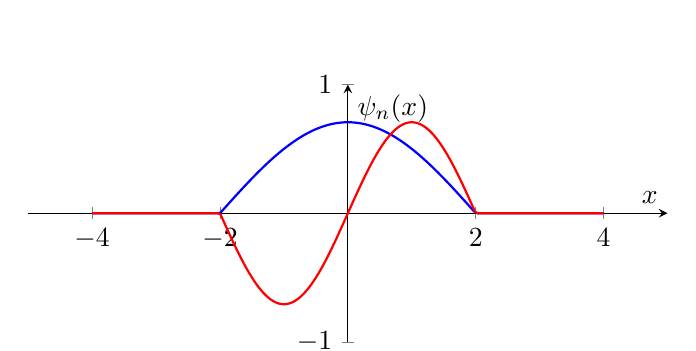
\begin{tikzpicture}
        \begin{axis}[
            axis lines = middle,
            xlabel = $x$,
            ylabel = {$\psi_n(x)$},
            ymin = -1,
            ymax = 1,
            xmin = -5,
            xmax = 5,
            xtick = {-4, -2, 0, 2, 4},
            ytick = {-1, 0, 1},
            domain = -4:4,
            samples = 200,
            width=0.8\textwidth,
            height=0.4\textwidth,
        ]
        \addplot[blue, thick] { (x < -2 || x > 2) * 0 + (x >= -2 && x <= 2) * (sqrt(2/4) * cos(deg(pi * 1 * x / (2 * 2)))) };
        \addplot[red, thick] { (x < -2 || x > 2) * 0 + (x >= -2 && x <= 2) * (sqrt(2/4) * sin(deg(pi * 2 * x / (2 * 2)))) };    
        \end{axis}
    \end{tikzpicture}
\end{figure}

It looks somehow weird that the energy eigenvalues are the same as a single infinite potential well of width $b$. This is because the two wells are completely isolated when $V_0 \to \infty$. In such case, there is no such even conditions anymore. So we juat take the single case solution here as the even one. When $V_0$ is finite, the wave functions in the two wells can overlap due to tunneling effect, leading to a splitting of the energy levels. The symmetric state $\ket S$ has a slightly lower energy than the antisymmetric state $\ket A$ due to constructive interference in the overlap region, while the antisymmetric state has a slightly higher energy due to destructive interference. This energy splitting is a hallmark of quantum tunneling in double well potentials.
We could disscuss the tunneling dynamics between the two wells as below.

Construct states $\ket R$ and $\ket L$ localized in the right and left wells respectively. 
\begin{align}
    \ket R &= \frac{1}{\sqrt 2} \left( \ket S + \ket A \right) \\
    \ket L &= \frac{1}{\sqrt 2} \left( \ket S - \ket A \right)
\end{align}
S,A denoting the symmetric and antisymmetric states. The tunneling between the two wells can be described by time evolution of the states:
\begin{align}
    \ket R(t) &= \frac{1}{\sqrt 2} \left( \ee^{- \ii E_S t / \hbar} \ket S + \ee^{- \ii E_A t / \hbar} \ket A \right) \\
    &= \frac{1}{\sqrt 2} \ee^{- \ii (E_S + E_A) t / 2 \hbar} \left( \ee^{- \ii (E_S - E_A) t / 2 \hbar} \ket S + \ee^{\ii (E_S - E_A) t / 2 \hbar} \ket A \right) \\
    &= \ee^{- \ii (E_S + E_A) t / 2 \hbar} \left[ \cos \left( \frac{E_A - E_S}{2 \hbar} t \right) \ket R - \ii \sin \left( \frac{E_A - E_S}{2 \hbar} t \right) \ket L \right]
\end{align}
At time $t = T/2$ determined by from above equation, we have
\begin{align}
    \ket R(T/2) = - \ii \ee^{- \ii (E_S + E_A) T / 4 \hbar} \ket L
\end{align}
indicating that the particle initially localized in the right well has tunneled to the left well 
\begin{align}
    T = \frac{2 \pi \hbar}{E_A - E_S}
\end{align}
\begin{ex}
    ammonia molecule NH$_3$ has a pyramidal structure with the nitrogen atom able to tunnel through the plane formed by the three hydrogen atoms. This tunneling leads to an inversion of the molecule, which can be modeled as a particle in a double well potential. The two wells correspond to the nitrogen atom being above or below the plane of hydrogen atoms. The energy splitting between the symmetric and antisymmetric states due to tunneling results in a characteristic frequency of inversion, which can be observed spectroscopically. This phenomenon is a classic example of quantum tunneling in molecular systems.
\end{ex}
\begin{figure}[h!]
    \centering
    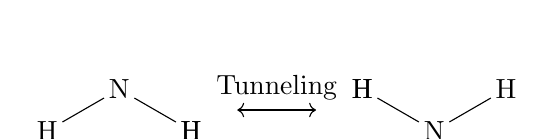
\begin{tikzpicture}
        % 左：N 在下方（H3 朝上）
        \node at (0,0)
            {\chemfig{N(-[:210]H)(-[:330]H)([:90]H)}};
        % 右：N 在上方（H3 朝下）
        \node at (4,0)
            {\chemfig{N(-[:30]H)(-[:150]H)([:-90]H)}};
        % 双箭头
        \draw[<->] (1.5,0) -- (2.5,0)
            node[midway,above]{Tunneling};
    \end{tikzpicture}
    \caption{Inversion of ammonia NH$_3$ due to tunneling of the N atom through the plane of H atoms.}
\end{figure}

The energy and parity eigenstates are superpositions of the localized states: 
\begin{align}
    \ket S &= \frac{1}{\sqrt 2} \left( \upket + \downket \right) \\
    \ket A &= \frac{1}{\sqrt 2} \left( \upket - \downket \right)
\end{align}

Naturally occuring organic molecules, such as amino acids, which are of R-type or L-type only. Such molecules with a definite handedness are called optical isomers. The oscillation time $(10^4 \text{ to } 10^6)$ is infinite for practical. Chiral can be determined by the polarized light rotation experiment. A synthesis in the labotatory yields equal amonut of $R-$ and $L-$ type

\emph{This is also Strum-Liouville theory}

\subsection{Parity Selection Rule}

Consider parity eigenstates $\ket \alpha$ and $\ket \alpha$ with eigenvalues $\lambda_{\alpha}, \lambda_{\beta} = \pm 1$. 
\begin{align}
    \oPi \ket \alpha = \lambda_{\alpha} \ket \alpha, \quad \oPi \ket \beta = \lambda_{\beta} \ket \beta
\end{align}
Consider the matrix element of potition operator $\ox$ between these two states:
\begin{align}
    \bra \alpha \ox \ket \beta &= \bra \alpha \oPi^ \dag \ox \oPi \ket \beta \notag \\
    &= - \bra \alpha \ox \ket \beta \notag \\
    & = 0 \quad \text{if } \lambda_{\alpha} \lambda_{\beta} = 1
\end{align}
But the reality is that $\ox$ is an odd operator under parity transformation, i.e., $\oPi^ \dag \ox \oPi = - \ox$. Thus the matrix element $\bra \alpha \ox \ket \beta$ vanishes unless the two states have opposite parity, i.e., $\lambda_{\alpha} \lambda_{\beta} = -1$. This result is known as the parity selection rule, which states that transitions between states of the same parity are forbidden for operators that are odd under parity transformation.

\subsection{Parity nonconservation}

$\beta$-decay: neutron decays into a proton, an electron and an anti-neutrino. The proton and neutron form an isospin doublet, and the weak interaction responsible for $\beta$-decay violates parity symmetry. This was first experimentally confirmed in the Wu experiment in 1957, which demonstrated that the distribution of emitted electrons in the decay of polarized cobalt-60 nuclei was not symmetric with respect to spatial inversion. This discovery had profound implications for our understanding of fundamental symmetries in physics and led to the realization that the weak interaction is not invariant under parity transformation. 

\newpage
\subsection{Lattice Translation}

Consider a periodic potential in 1d, with $V(x) = V(x+a)$, as shown in \cref{fig:periodic_lattics}.

\begin{figure}[h!]
    \centering
    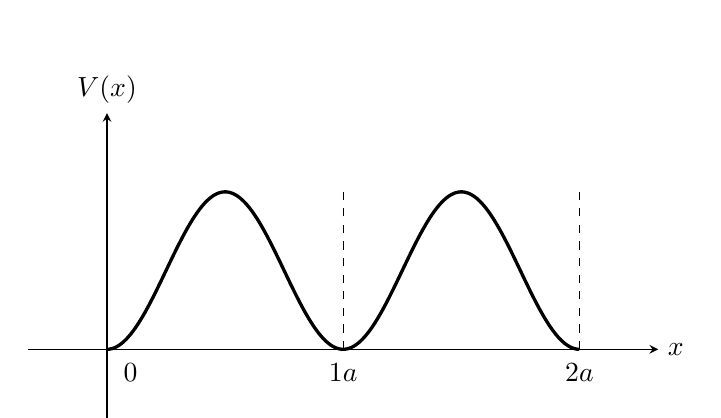
\begin{tikzpicture}[>=stealth, scale=1]
        \draw[->] (-1,0) -- (7,0) node[right] {$x$};
        \draw[->] (0,-1) -- (0,3) node[above] {$V(x)$};
        \node at (0.3,-0.3) {0};
        \draw[very thick, domain=0:6, samples=200] plot (\x, {2*sin(deg(pi*\x/3))^2});
        \foreach \i in {1,2} {
            \draw[dashed] (3*\i,0) -- (3*\i,2);
            \node at (3*\i, -0.3) {\( \i a \)};
        }
    \end{tikzpicture}
    \caption{Periodic potential with period $a$.}
    \label{fig:periodic_lattics}
\end{figure}

Such a potential may describe the motion of an electron in a chain of regularly spcaed ions. In general the Hamiltonian is not invariant under a translation by an arbitrary length $l$ as the definition of a translation operaotr in \cref{sec:translation_symmetry}. However, the Hamiltonian is invariant under a translation by an integer multiple of the lattice constant $a$.
This is because the potential satisfies $V(x+na) = V(x)$ for any integer $n$. As a result, the energy eigenstates of the Hamiltonian can be chosen to be simultaneous eigenstates of the lattice translation operator $\oT(na)$. 
\begin{align}
    &\oT_a^ \dag V(\ox) \oT_a = V (\ox+a) = V(\ox)  \\
    \implies & {\oT_a^ {\dag n}} V(\ox) {\oT_a}^n = V(\ox +na) = V(\ox)
\end{align}
The kinetic energy in Hamiltonian is invariant under arbitrary displacement, the entire Hamiltonian satisfies
\begin{align}
    \oT_a^ \dag \oH \oT_a = \oH 
\end{align}
And we know that the translation operator is an unitary operator 
\begin{align}
    \oH \oT_a - \oT_a \oH = 0 \implies \comm{\oH}{\oT_a} = 0
\end{align}
Such that the Hamiltonian and Lattice Translation Operators can be simultaneously diagonalized for this reason. 

Now consider a periodic potential with infinitely high boundaries. 
\begin{figure}[h!]
    \centering
    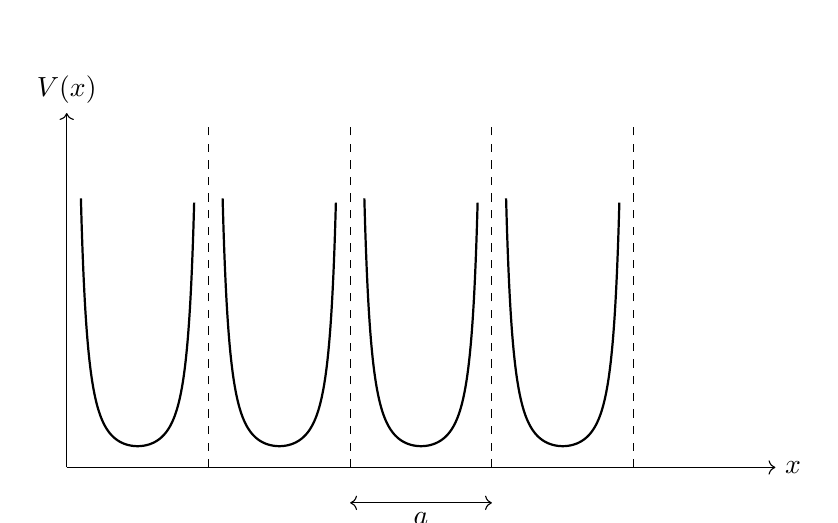
\begin{tikzpicture}[scale=0.9]

  % 坐标轴
  \draw[->] (0,0) -- (10,0) node[right] {$x$};
  \draw[->] (0,0) -- (0,5) node[above] {$V(x)$};

  % 晶格周期边界（虚线）
  \foreach \x in {2,4,6,8}{
    \draw[dashed] (\x,0) -- (\x,4.8);
  }

  % 每个势阱：在边界处势能发散（用 1/(x-x_0)^2 型函数表示）
    \draw[thick,smooth,domain=2.2:3.8,samples=150]
    plot (\x,{0.15*(1/((\x-2)^2)+1/((4-\x)^2))});
    \draw[thick,smooth,domain=4.2:5.8,samples=150]
    plot (\x,{0.15*(1/((\x-4)^2)+1/((6-\x)^2))});
    \draw[thick,smooth,domain=6.2:7.8,samples=150]
    plot (\x,{0.15*(1/((\x-6)^2)+1/((8-\x)^2))});
    \draw[thick,smooth,domain=0.2:1.8,samples=150]
    plot (\x,{0.15*(1/((\x-0)^2)+1/((2-\x)^2))});
  % 周期 a 标注
  \draw[<->] (4,-0.5) -- (6,-0.5)
    node[midway,below] {$a$};

    \end{tikzpicture}
    \caption{Periodic potential with infinitely high boundaries.}
    \label{fig:periodic_lattics_infinite}
\end{figure}

A particle located at the lattice site $n$ is a ground state of the Hamiltonian. We denote this state by $\ket{n}$, $\oH \ket{n} = E_0 \ket{n}$. The wave function $\braket{x'|n}$ is finite only on the n-th lattice site\footnote{We can see that the potential will go to infinite at each edge of the lattice}. $\ket{n}$ is not an eigenstate of $\oT_a$: 
\begin{align}
    \oT_a \ket{n} = \ket{n+1}
\end{align}
This is possible as the energy eigenstates of the Hamiltonian can be degenerate. And because of the potential well is infinitely high at the boundaries, so each lattice site is isolated. Consider a new state defined as 
\begin{align}
    \ket{\theta} \equiv \sum_{n=-\infty}^{\infty} \ee^{\ii n \theta} \ket{n} \quad \theta \in [-\pi, \pi]
\end{align}
The choice of the phase factor $\ee^{\ii n \theta}$ is to ensure that $\ket{\theta}$ is an eigenstate of the lattice translation operator $\oT_a$:
\begin{align}
    \oT_a \ket{\theta} &= \sum_{n=-\infty}^{\infty} \ee^{\ii n \theta} \oT_a \ket{n} = \sum_{n=-\infty}^{\infty} \ee^{\ii n \theta} \ket{n+1} \notag \\
    &= \ee^{- \ii \theta} \sum_{m=-\infty}^{\infty} \ee^{\ii m \theta} \ket{m} = \ee^{- \ii \theta} \ket{\theta}
\end{align}
For last line we have made a change of variable $m = n+1$. Thus $\ket{\theta}$ is an eigenstate of $\oT_a$ with eigenvalue $\ee^{- \ii \theta}$. Since $\oH \ket{n} = E_0 \ket{n}$ for all $n$, we have 
\begin{align}
    \oH \ket{\theta} &= \sum_{n=-\infty}^{\infty} \ee^{\ii n \theta} \oH \ket{n} = E_0 \sum_{n=-\infty}^{\infty} \ee^{\ii n \theta} \ket{n} = E_0 \ket{\theta}
\end{align}
Thus $\ket{\theta}$ is also an eigenstate of the Hamiltonian with eigenvalue $E_0$. Therefore, we have constructed a set of simultaneous eigenstates of both the Hamiltonian and the lattice translation operator, labeled by the continuous parameter $\theta$. The eigenvalue of the lattice translation operator is $\ee^{- \ii \theta}$, which lies on the unit circle in the complex plane.
\begin{figure}[h!]
    \centering
    \begin{tikzpicture}[scale=2]
        % Draw the unit circle
        \draw[thick] (0,0) circle(1);
        
        % Draw the axes
        \draw[->] (-1.5,0) -- (1.5,0) node[right] {Re};
        \draw[->] (0,-1.5) -- (0,1.5) node[above] {Im};
        
        % Draw the angle theta
        \draw[thick,->] (0,0) -- (0.866,0.5) node[midway, above right] {$\theta$};
        
        % Mark the point on the unit circle
        \filldraw[red] (0.866,0.5) circle(0.05) node[above right] {$e^{-i\theta}$};
        
        % Draw dashed lines to axes
        \draw[dashed] (0.866,0) -- (0.866,0.5);
        \draw[dashed] (0,0.5) -- (0.866,0.5);
        
        % Label the angle
        \draw (0.3,0) arc(0:30:0.3);
        \node at (0.4,0.1) {$\theta$};
    \end{tikzpicture}
    \caption{Eigenvalue $e^{-i\theta}$ of the lattice translation operator $\oT_a$ on the complex unit circle.}
\end{figure}

But for this case, the wave fucntions are only localized at each lattice site, there is no overlap between different sites, thus the energy eigenvalue is degenerate and independent of $\theta$. In a more realistic scenario where the potential wells have finite depth, as shown in \cref{fig:Lattice_finite_wavefunction} , the wave functions can overlap between neighboring lattice sites due to quantum tunneling(or to say the wavefunction have tails extending to neighboring sites). This overlap leads to a dependence of the energy eigenvalues on the parameter $\theta$, resulting in the formation of energy bands characteristic of electrons in crystalline solids.

\begin{figure}[h!]
    \centering
    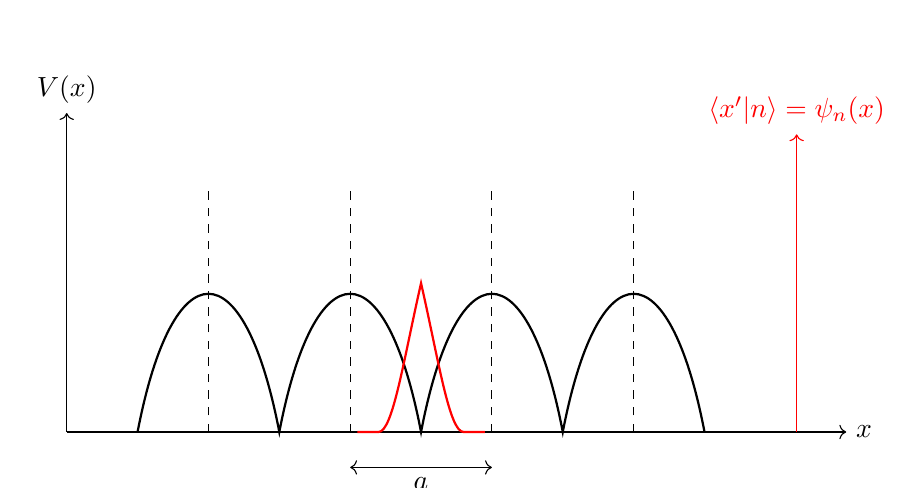
\begin{tikzpicture}[scale=0.9]

  % axes
  \draw[->] (0,0) -- (11,0) node[right] {$x$};
  \draw[->] (0,0) -- (0,4.5) node[above] {$V(x)$};

  % periodic potential (schematic bumps)
  \draw[thick]
    (1,0) .. controls (1.5,2.6) and (2.5,2.6) .. (3,0)
          .. controls (3.5,2.6) and (4.5,2.6) .. (5,0)
          .. controls (5.5,2.6) and (6.5,2.6) .. (7,0)
          .. controls (7.5,2.6) and (8.5,2.6) .. (9,0);

  % cell boundaries (dashed)
  \foreach \x in {2,4,6,8}{
    \draw[dashed] (\x,0) -- (\x,3.4);
  }

  % localized wave function in one well
  \draw[red,thick]
    (4.1,0) -- (4.4,0)
      .. controls (4.6,0)   and (4.75,1.0) .. (5,2.1)
      .. controls (5.25,1.0) and (5.4,0)   .. (5.6,0)
    -- (5.9,0);

  % lattice spacing a
  \draw[<->] (4,-0.5) -- (6,-0.5)
    node[midway,below] {$a$};

  % vertical axis for wave function
  \draw[->,red] (10.3,0) -- (10.3,4.2)
    node[above] {$\langle x'|n\rangle = \psi_n(x)$};

\end{tikzpicture}
\caption{Periodic finite lattice potential and wave function on lattice n}
\label{fig:Lattice_finite_wavefunction}
\end{figure}

The diagonal matrix elements of the Hamiltonian $\bra{n} \oH \ket{n} = E_0$ must be all equal as the translation invariance. 
We suppose that the only non-diagnoal elements of importance are the one connecting immediate neighbors.
\begin{align}
    \bra{n'} \oH \ket{n} \geq 0 \text{ iff } n'=n, n \pm 1
\end{align}
Such assumption is called the \emph{tight-binding approximation}, which is valid when the overlap between wave functions on non-neighboring sites is negligible, also could be written as 
\begin{align}
    \bra{n+1} \oH \ket{n} = - \Delta
\end{align}
which is independent of $n$ due to translation invariance. Under this approximation, we can write the action of the Hamiltonian on the state $\ket{n}$ as
\begin{align}
    \oH \ket n = E_0 \ket n - \Delta \ket {n+1} - \Delta \ket {n-1}
\end{align}
We can now again form the linear combination state $\ket \theta$ as before, 
\begin{align}
    \ket{\theta} = \sum_n \ee^{\ii n \theta} \ket n \quad \& \quad \oT_a \ket{\theta} = \ee^{- \ii \theta} \ket{\theta}
\end{align}
Applying the Hamiltonian to $\ket \theta$, we have
\begin{align}
    \oH \ket \theta &= \sum_n \ee^{\ii n \theta} \oH \ket n \notag \\
    &= \sum_n \ee^{\ii n \theta} \left( E_0 \ket n - \Delta \ket {n+1} - \Delta \ket {n-1} \right) \notag \\
    &= E_0 \sum_n \ee^{\ii n \theta} \ket n - \Delta \sum_n \ee^{\ii n \theta} \ket {n+1} - \Delta \sum_n \ee^{\ii n \theta} \ket {n-1} \notag \\
    &= E_0 \ket{\theta} - \Delta \ee^{- \ii \theta} \sum_m \ee^{\ii m \theta} \ket m - \Delta \ee^{\ii \theta} \sum_l \ee^{\ii p \theta} \ket l \notag \\
    &= E_0 \ket{\theta} - \Delta (\ee^{- \ii \theta} + \ee^{\ii \theta}) \ket{\theta} \\ 
    &= \left[ E_0 - 2 \Delta \cos(\theta) \right] \ket{\theta}
\end{align}
The eigenstate depend on the parameter $\theta$. The degeneracy is lifted, and we have a contineous spectrum of eigenvalues between $E_0 - 2 \Delta$ and $E_0 + 2 \Delta$. 

Consider the wavefunction $\braket{x'|\theta}$. For the translated state $\oT_a \theta$, we have 
\begin{align}
    \bra{x'} \oT_a \ket{\theta} & = \left( \bra{x'} \oT_{-a}^ \dag \right)\ket{\theta} \notag \\
    &= \braket{x'-a|\theta} 
\end{align}
Together with the eigenvalue equation of $\oT_a$, we have
\begin{align}
    \braket{x'-a|\theta} = \ee^{- \ii \theta} \braket{x'|\theta}
\end{align}
We find a solution by making the ansatz
\begin{align}
    \braket{x'|\theta} = \ee^{\ii k x'} u_k(x') \text{ with } \theta = k a \text{ and } u_k(x'\pm a) = u_k(x')
\end{align}
We can verify that this ansatz satisfies the above equation: 
\begin{align}
    \braket{x'-a|\theta} &= \ee^{\ii k (x'-a)} u_k(x'-a) \notag \\
    &= \ee^{\ii k (x'-a)} u_k(x') \notag \\
    &= \ee^{- \ii k a} \ee^{\ii k x'} u_k(x') \notag \\
    &= \ee^{- \ii k a} \braket{x'|\theta}
\end{align}
For wave functions in a periodic potential, we therefore find the condition known as \emph{Bloch Theorem}: 
\begin{theorem}[Bloch Theorem]
    The energy eigenstates of a particle in a periodic potential can be expressed in the form
    \begin{align}
        \psi_k(x) = \braket{x|k} = \ee^{\ii k x} u_k(x)
    \end{align}
    where $u_k(x)$ is a function with the same periodicity as the potential, i.e., $u_k(x+a) = u_k(x)$ for all $x$. Here, $k$ is the crystal momentum, which lies within the first Brillouin zone, typically defined as $-\pi/a \leq k < \pi/a$.
\end{theorem}




\newpage






\subsection{Time-Reversal Discrete Symmetry}

The conception of time-reversal is sound somehow scientific puuzle. What dose it exactly mean? Let us consider a different example: position-reversal. Consider a particle move a along a curve(also its trajectory) which is parameterized by time $t$. At time $t=0$, we let the  paricle stop and reverse its motion, the position and momentum is then be $x|_{t=0_-} = -x|_{t=0_+} $
, $p|_{t=0_+} = p|_{t=0_-}$. The particle then move back along the same curve but in the opposite direction. 
\begin{figure}[h!]
    \centering
    \tikzset{every picture/.style={line width=0.75pt}} %set default line width to 0.75pt        

\begin{tikzpicture}[x=0.75pt,y=0.75pt,yscale=-1,xscale=1]
%uncomment if require: \path (0,300); %set diagram left start at 0, and has height of 300

%Curve Lines [id:da5488504090671414] 
\draw    (163,113) .. controls (203,104) and (305,220) .. (308,252) ;
%Curve Lines [id:da023649926549646594] 
\draw    (305,110) .. controls (345,101) and (447,217) .. (450,249) ;
\draw   (190.86,127.99) .. controls (197.77,127.39) and (203.68,128.26) .. (208.56,130.57) .. controls (204.7,126.8) and (201.85,121.55) .. (200.01,114.86) ;
\draw   (363.21,127.48) .. controls (356.28,127.79) and (350.42,126.67) .. (345.64,124.15) .. controls (349.34,128.09) and (351.97,133.45) .. (353.52,140.21) ;
\draw   (209.26,142.42) .. controls (216.27,142.12) and (222.31,143.23) .. (227.38,145.72) .. controls (223.28,141.83) and (220.16,136.54) .. (218.01,129.86) ;
\draw   (223.72,154.84) .. controls (230.65,154.95) and (236.44,156.42) .. (241.06,159.22) .. controls (237.6,155.07) and (235.3,149.56) .. (234.16,142.72) ;
\draw   (346.09,116.76) .. controls (339.19,117.51) and (333.27,116.78) .. (328.34,114.57) .. controls (332.28,118.26) and (335.25,123.44) .. (337.24,130.09) ;
\draw   (382.31,144.77) .. controls (375.39,144.28) and (369.69,142.51) .. (365.23,139.46) .. controls (368.46,143.79) and (370.46,149.42) .. (371.23,156.31) ;
%Shape: Circle [id:dp870416844684753] 
\draw  [fill={rgb, 255:red, 0; green, 0; blue, 0 }  ,fill opacity=1 ] (259,178.5) .. controls (259,177.67) and (259.67,177) .. (260.5,177) .. controls (261.33,177) and (262,177.67) .. (262,178.5) .. controls (262,179.33) and (261.33,180) .. (260.5,180) .. controls (259.67,180) and (259,179.33) .. (259,178.5) -- cycle ;
%Shape: Circle [id:dp9542782425706763] 
\draw  [fill={rgb, 255:red, 0; green, 0; blue, 0 }  ,fill opacity=1 ] (407,178.5) .. controls (407,178.67) and (406.33,178) .. (405.5,178) .. controls (404.67,178) and (404,178.67) .. (404,179.5) .. controls (404,180.33) and (404.67,181) .. (405.5,181) .. controls (406.33,181) and (407,180.33) .. (407,179.5) -- cycle ;

% Text Node
\draw (269,170) node [anchor=north west][inner sep=0.75pt]    {$\mathrm{t} =0$};
% Text Node
\draw (417,170) node [anchor=north west][inner sep=0.75pt]    {$\mathrm{t} =0$};
% Text Node
\draw (121,79) node [anchor=north west][inner sep=0.75pt]   [align=left] {Before reversal};
% Text Node
\draw (277,80) node [anchor=north west][inner sep=0.75pt]   [align=left] {After reversal};


\end{tikzpicture}
\caption{Position-reversal of a particle along its trajectory.}
\end{figure}

Generally speaking, if $x(t)$ is a solution of Newton's equation of motion, then so is $-x(-t)$.
\begin{align}
    t'=t \implies \ddx{t'} = - \ddx{t} \implies \ddxx{}{{t'}} = \ddxx{}{t}
\end{align}

We now consider time-reversal, with a similar consideration by Schrödinger equation \cref{eq:time_dependent_schrodinger_equation}. When we have a solution $\psi(x,t)$, the time-reversed solution is given by $\psi^*(x,-t)$. There is a bit difference here compared to Newton's equation of motion, now let's see why we need to take the complex conjugate. Take the so called pre-time-reversal operator $\oT_p$ which just simply reverse the time $t \to -t$, we have the time-dependent Schrödinger equation as
\begin{align*}
    \ii \hbar \pdv{\psi(x,-t)}{(-t)} = \oH \psi(x,-t) \\
    - \ii \hbar \pdv{\psi(x,-t)}{t} = \oH \psi(x,-t)
\end{align*}
This is not the concrete time-reversed Schrödinger equation, as the sign in front of the imaginary unit is different. To fix this, we need to take the complex conjugate of the wave function, leading to the true time-reversed wave function $\psi^*(x,-t)$. Taking the complex conjugate of the above equation, we have
\begin{align*}
    \ii \hbar \pdv{\psi^*(x,-t)}{t} = \oH \psi^*(x,-t)
\end{align*}

Now we have the correct time-reversed Schrödinger equation. Thus the time-reversal operator $\oThe$ can cause a transformation on the wave function not just by reversing the time, but also taking the complex conjugate:
\begin{align*}
    \oThe \psi(x,t) = \psi^*(x,-t)
\end{align*}

Before we proceed to find the eigenvalue and eigenstate of the time-reversal operator, we first check whether the time-reversal operator is a linear operator. Consider a linear combination of two wave functions $\psi_1(x,t)$ and $\psi_2(x,t)$, we have
\begin{align*}
    \oThe \left( a \psi_1(x,t) + b \psi_2(x,t) \right) &= a \psi_1^*(x,-t) + b \psi_2^*(x,-t) \\
    &\neq a \oThe \psi_1(x,t) + b \oThe \psi_2(x,t)
\end{align*}
Thus the time-reversal operator is not a linear operator, but an anti-linear operator due to the complex conjugation.

As we are actually talking about the symmetry. So let us introduce a important theorem here.
\begin{theorem}[Wigner's Theorem]
    Any symmetry transformation in quantum mechanics can be represented by either a unitary operator or an anti-unitary operator acting on the Hilbert space of states.
\end{theorem}
\begin{proof}
    Consider a symmetry transformation $\oS$ that maps state vectors in the Hilbert space to other state vectors. 
    By definition of a symmetry in quantum mechanics it must preserve all transition probabilities, i.e.\ for any two state vectors $\ket{\psi}$ and $\ket{\phi}$ we require
    \begin{align*}
        \abs{\braket{\psi|\phi}}^2 = \abs{\braket{\oS\psi|\oS\phi}}^2 .
    \end{align*}
    In particular, this implies that norms are preserved,
    \begin{align*}
        \braket{\psi|\psi} = \braket{\oS\psi|\oS\psi},
    \end{align*}
    and that the absolute value of every inner product is unchanged. 
    Physically, the operation $\oS$ may change phases, but it cannot change any probability.

    From this preservation of the inner product structure one can show that there are only two possibilities for how $\oS$ acts on superpositions of states: for any complex numbers $a,b$ and any states $\ket{\psi},\ket{\phi}$,
    \begin{align}
        \oS \bigl(a \ket{\psi} + b \ket{\phi}\bigr)
        = a\, \oS \ket{\psi} + b\, \oS \ket{\phi}
        \label{eq:wigner-linear}
    \end{align}
    (the \emph{linear} case), or
    \begin{align}
        \oS \bigl(a \ket{\psi} + b \ket{\phi}\bigr)
        = a^* \oS \ket{\psi} + b^* \oS \ket{\phi}
        \label{eq:wigner-antilinear}
    \end{align}
    (the \emph{anti-linear} case).  
    The idea of the proof is that, since probabilities for all superpositions must be preserved, the relative phases in a superposition can only be kept as they are [case \eqref{eq:wigner-linear}] or be complex–conjugated [case \eqref{eq:wigner-antilinear}]. 
    No other dependence on $a$ and $b$ is compatible with the requirement that all transition probabilities remain the same.

    Next we choose an orthonormal basis $\{\ket{e_i}\}$ of the Hilbert space.  
    Because $\oS$ preserves norms and the absolute values of inner products, the transformed vectors $\{\oS\ket{e_i}\}$ also form an orthonormal set. 
    We now define an operator by its action on this basis.

    If $\oS$ is linear as in \eqref{eq:wigner-linear}, we define a linear operator $\oU$ by
    \begin{align*}
        \oU \ket{e_i} = \oS \ket{e_i} .
    \end{align*}
    Extending $\oU$ linearly to the whole space, we have for arbitrary states
    \begin{align*}
        \braket{\oU\psi|\oU\phi} = \braket{\psi|\phi},
    \end{align*}
    since the matrix elements in the basis $\{\ket{e_i}\}$ are unchanged. 
    Thus $\oU$ is a norm– and inner–product–preserving linear map, i.e.\ a unitary operator.

    If instead $\oS$ is anti-linear as in \eqref{eq:wigner-antilinear}, we define an anti-linear operator $\oA$ by
    \begin{align*}
        \oA \ket{e_i} = \oS \ket{e_i} ,
    \end{align*}
    and extend it anti-linearly. 
    One then finds
    \begin{align*}
        \braket{\oA\psi|\oA\phi} = \braket{\psi|\phi}^* ,
    \end{align*}
    so $\oA$ preserves norms and complex–conjugates inner products. 
    Such an operator is called \emph{anti-unitary}.

    In summary, any symmetry transformation $\oS$ that preserves transition probabilities can be represented on the Hilbert space either by a unitary operator $\oU$ or by an anti-unitary operator $\oA$. 
    This is Wigner's theorem.
\end{proof}
Wigner's theorem tells us that symmetries in quantum mechanics can be represented by operators that preserve the inner product structure of the Hilbert space, either through linear (unitary) or anti-linear (anti-unitary) transformations. Since the time-reversal operator is anti-linear, it must be represented by an anti-unitary operator according to Wigner's theorem.

For this reason, the time-reversal operator $\oThe$ is an anti-unitary operator can be expressed as the product of a unitary operator $\oU$ and the complex conjugation operator $\oK$, i.e.,
\begin{align}
    \oThe = \oU \oK
\end{align}

where $\oK$ acts on a vector $c\ket{\psi}$ with $c \in \C$ by taking its complex conjugate:
\begin{align}
    \oK \left( c \ket{\psi} \right) = c^* \ket{\psi}
\end{align}
If $\ket{\psi}$ could be expanded in a basis $\{ \ket{n} \}$ as $\ket{\psi} = \sum_n \ket{n} \braket{n|\psi}$, then the action of $\oK$ on $\ket{\psi}$ is given by
\begin{align}
    \oK \ket{\psi} = \sum_n \braket{n|\psi}^* \ket{n} \label{eq:complex_conjugation_operator}
\end{align}

Let us check the anti-linearity of $\oThe$
\begin{align*}
    \oThe \left(c_1 \kps + c_2 \kph\right) &= \oU \oK \left(c_1 \kps + c_2 \kph\right) \\
    &= \oU \left(c_1^* \oK \kps + c_2^* \oK \kph\right) \\
    &= c_1^* \oU \oK \kps + c_2^* \oU \oK \kph \\
    &= c_1^* \oThe \kps + c_2^* \oThe \kph
\end{align*}

As the form \cref{eq:complex_conjugation_operator}, we can see that it is safer to not consider the action of $\oThe$ on bras of the Hermitian adjoint $\oThe^ \dag$. Consider the transformed vector 
\begin{align*}
    &\oThe \kps = \sum_n \braket{n|\psi}^* \oU \ket{n} = \sum_n \braket{\psi|n} \oU \ket{n} \\
    &\oThe \kph = \sum_n \braket{n|\phi}^* \oU \ket{n} = \sum_n \braket{\phi|n} \oU \ket{n} \\
    \implies & \braket{\oThe \psi|\oThe \phi} = \sum_{m,n} \braket{\psi|m}^* \braket{n|\phi} \bra{m} \oU^ \dag \oU \ket{n} \\
    &= \sum_{m,n} \braket{\psi|m}^* \braket{n|\phi} \delta_{mn} = \sum_n \braket{\psi|n}^* \braket{n|\phi} \\
    &= \left( \sum_n \braket{n|\psi} \braket{\phi|n} \right)^* = \braket{\phi|\psi}^*
\end{align*}
Now we could say, an anti-unitary operator $\oThe$ satisfies such kind of decomposition of inner product.
\subsection{Time-Reversal Operator}

We now consider the time-reversal operator $\oThe$ in more detail. The time-reversal operator could be considered by time evolution operator. Consider a infinitesimal $\delta t$ we have
\begin{align*}
    \ket{\psi;t_0=0,t= \delta t} = \left(1 - \frac{\ii \oH}{\hbar} \delta t\right)
\end{align*}
with an initial state $\ket{\psi;0,0} = \ket{\psi}$. The time evolution of the time-reversed state is given by
\begin{align*}
    \left(1 - \frac{\ii \oH}{\hbar} \delta\right) \oThe \kps
\end{align*}
If the motion is symmetry under time-reversal, then the state $\oThe \ket{\psi; t_0 =0, t= \delta t}$ is the same state as $\ket{\psi; t_0 =0, t= - \delta t}$, we have
\begin{align*}
    \oThe \left(1 - \frac{\ii \oH}{\hbar} \delta t\right) \kps = \left(1 - \frac{\ii \oH}{\hbar} \delta t\right) \oThe \kps
\end{align*}
If the relation is true for arbitrary $\ket{\psi}$, if $\oThe$ is unitary we have
\begin{align*}
    - \ii \oH \oThe = \ii \oThe \oH \implies \anticomm{\oH}{\oThe} = 0
\end{align*}

Consider now an energy eigenstate $\ket n$ with eigenvalue $E_n$. Then, the time reversed state $\oThe \ket{n}$ satisfies 
\begin{align*}
    \oH \oThe \ket{n} &= - \oThe \oH \ket{n} \notag \\
    &= - E_n \oThe \ket{n}
\end{align*}

Thus $\oThe \ket{n}$ is also an energy eigenstate with the same eigenvalue $-E_n$. This is not possible even in the elementary case of a free particle: the spectrum $\frac{\hbar^2 k^2 }{2m}$ is positive semidefinite and thus not contain negative eigenvalues.
Such that the time-reversal operator $\oThe$ must be anti-unitary. Then 
\begin{align*}
    - \ii \oH \oThe = \oThe \ii \oH = - \ii \oThe \oH \implies \comm{\oH}{\oThe} = 0
\end{align*}
The Hamiltonian is commutative with the time-reversal operator. Also called time-reversal symmetry of Hamiltonian.

Now consider a general operator $\oO$, and want to find how it transforms under time-reversal. Firstly give the expression and then proof it. 
\begin{align}
    \bra{\phi} \oO \kps = \bra{\oThe \psi} \oThe \oO \oThe^{-1} \ket{\oThe \phi} \label{eq:time_reversal_operator_transformation} 
\end{align}
\begin{proof}
    Define $\ket{\phi'} \equiv \oO^ \dag \ket{\phi}$, the corresponding bra is $\bra{\phi'} = \bra{\phi} \oO$. Then using $\ket{ \oThe\phi'} = \oThe \ket{\phi'}$, we have
    \begin{align*}
        \bra{\phi} \oO \kps & = \braket{\phi'|\psi} = \braket{\oThe \psi| \oThe \phi'} \\
        &= \bra{\oThe \psi} \oThe \oO^ \dag \ket{\phi} = \bra{\oThe \psi} \oThe \oO^ \dag \oThe^{-1} \ket{\oThe \phi} 
    \end{align*}
    For the first line we have used the anti-unitary property of $\oThe$.
\end{proof}

Such that, given a Hermitian operator $\oA$, we find 
\begin{align}
    \bra{\phi} \oA \kps = \bra{\oThe \psi} \oThe \oA \oThe^{-1} \ket{\oThe \phi} \label{eq:trs_hermitian}
\end{align}
We define an oberservable $\oA$ to be even or odd under time-reversal according to whether the upper or lower sign in the following relation holds:
\begin{align*}
    \oThe \oA \oThe^{-1} = \pm \oA
\end{align*}
Plug in this realtion to \cref{eq:trs_hermitian}, we have
\begin{align*}
    \bra{\phi} \oA \kps = \pm \bra{\oThe \psi} \oA \ket{\oThe \phi}
\end{align*}

For example, the position operator $\ox$ is even under time-reversal:
\begin{align}
    \oThe \ox \oThe^{-1} = \ox \label{eq:position_time_reversal}
\end{align}
This is because the position of a particle does not change sign when time is reversed; if a particle is at position $x$ at time $t$, it remains at position $x$ at time $-t$.
On the other hand, the momentum operator $\op$ is odd under time-reversal:
\begin{align}
    \oThe \op \oThe^{-1} = - \op \label{eq:momentum_time_reversal}
\end{align}

The commutation relation between postion and momentum operators is preserved under time-reversal:
\begin{proof}
    The commutation relation acting on an arbitrary ket is given by 
    \begin{align*}
        \comm{\ox_i}{\op_j} \ket{\alpha} = \ii \hbar \delta_{ij} \ket{\alpha}
    \end{align*}
    Applying the time-reversal transformation to both sides, we have 
    \begin{align*}
        \oThe \comm{\ox_i}{\op_j} \oThe^{-1} \oThe \ket{\alpha} &=  \oThe \ii \hbar \delta_{ij} \ket{\alpha} \notag \\
        \comm{\oThe \ox_i \oThe^{-1}}{\oThe \op_j \oThe^{-1}} \oThe \ket{\alpha} &= - \ii \hbar \delta_{ij} \oThe \ket{\alpha} \notag \\
        \comm{\ox_i}{- \op_j} \oThe \ket{\alpha} &= - \ii \hbar \delta_{ij} \oThe \ket{\alpha} \notag \\
        - \comm{\ox_i}{\op_j} \oThe \ket{\alpha} &= - \ii \hbar \delta_{ij} \oThe \ket{\alpha} \notag \\
        \comm{\ox_i}{\op_j} \oThe \ket{\alpha} &= \ii \hbar \delta_{ij} \oThe \ket{\alpha}
    \end{align*}
    Such that the commutation relation is preserved under time-reversal.
\end{proof}

The angular momentum operator $\oL_i = \ii \hbar \epsilon_{ijk} x_j p_k $ is also odd under time-reversal: 
\begin{align}
    \oThe \oL_i \oThe^{-1} &= \oThe \left( \ii \hbar \epsilon_{ijk} x_j p_k \right) \oThe^{-1} \notag \\
    &= \ii \hbar \epsilon_{ijk} \left( \oThe x_j \oThe^{-1} \right) \left( \oThe p_k \oThe^{-1} \right) \notag \\
    &= \ii \hbar \epsilon_{ijk} x_j (- p_k) \notag \\
    &= - \oL_i \label{eq:angular_momentum_time_reversal}
\end{align}

We consider a spinless particle to be in state $\ket{\alpha}$. In position representation, we can expand 
\begin{align*}
    \ket{\alpha} = \int \dd^3 x' \braket{x'|\alpha} \ket{x'}
\end{align*}
Application of the time-reversal operator yields 
\begin{align*}
    \oThe \ket{\alpha} &= \oThe \int \dd^3 x' \braket{x'|\alpha} \ket{x'} \notag \\
    &= \int \dd^3 x' \braket{x'|\alpha}^* \oThe \ket{x'} \notag \\
    &= \int \dd^3 x' \braket{x'|\alpha}^* \ket{x'}
\end{align*}
the $\braket{x'|\alpha}^*$ is the wavefunction of the time-reversed state in position representation. 

The eigenfunction of angular momentum operator in central potential is given by
\begin{align*}
    \psi_{n l m}(r, \theta, \phi) = R_{n l}(r) Y_{l}^m(\theta, \phi)
\end{align*}
where $R_{n l}(r)$ is the radial wave function and $Y_{l}^m(\theta, \phi)$ is the spherical harmonic function. Under time-reversal, the wave function transforms as
\begin{align*}
    \psi_{n l m}(r, \theta, \phi) \to \psi_{n l m}^*(r, \theta, \phi) = R_{n l}(r) Y_{l}^{m*}(\theta, \phi) 
\end{align*}
The radial wave function $R_{n l}(r)$ is real-valued, so it remains unchanged under time-reversal. However, the spherical harmonic function $Y_{l}^m(\theta, \phi)$ generally has complex values and transforms to its complex conjugate $Y_{l}^{m*}(\theta, \phi)$ under time-reversal.
Using the property of spherical harmonics $\ylm{l}{m}(\theta,\phi) \propto \ee^{\ii m \phi} P^{m}_l (\cos \theta)$ where $P^{m}_l (\cos \theta)$ is the associated Legendre polynomial, we find that under time-reversal, the azimuthal dependence $\ee^{\ii m \phi}$ transforms to $\ee^{-\ii m \phi}$. This effectively changes the magnetic quantum number $m$ to $-m$. Also the Legendre polynomial satisfies the relation $P^{m}_l (\cos \theta) = (-1)^m  P^{-m}_l (\cos \theta)$, we have
\begin{align*}
    Y_{l}^{m*}(\theta, \phi) = (-1)^m Y_{l}^{-m}(\theta, \phi)
\end{align*}
Such that we can deduce the action of time-reversal operator on the angular momentum eigenstate as
\begin{align}
    \oThe \ket{n, l, m} = (-1)^m \ket{n ,l, -m} \label{eq:time_reversal_angular_momentum_eigenstate}
\end{align}

Consider the probability current density $\bfvec{j}(\bfvec{r},t)$ associated with the eigenfunction of type $ \psi \propto R_{nl}\ylm{l}{m}$ as 
\begin{align*}
    \bfvec{j}(\bfvec{r},t) &= \frac{\hbar}{2 \ii m} \left( \psi^* \nabla \psi - \psi \nabla \psi^* \right) \\
    &= \frac{\hbar}{2 \ii m} \left( R_{nl} Y_{l}^{m*} \nabla (R_{nl} Y_{l}^{m}) - R_{nl} Y_{l}^{m} \nabla (R_{nl} Y_{l}^{m*}) \right) \\
    &= \frac{\hbar}{2 \ii m} R_{nl}^2 \left( Y_{l}^{m*} \nabla Y_{l}^{m} - Y_{l}^{m} \nabla Y_{l}^{m*} \right) \\
    & = \frac{\hbar}{2 \ii m} R^2_{nl} \left( (-1)^m \ylm{l}{-m} \nabla \ylm{l}{m} - (-1)^m \ylm{l}{m} \nabla \ylm{l}{-m} \right)
\end{align*}
If we change $m \to -m$, we have
\begin{align*}
    \bfvec{j}(\bfvec{r},t) &\to \frac{\hbar}{2 \ii m} R^2_{nl} \left( (-1)^{-m} \ylm{l}{m} \nabla \ylm{l}{-m} - (-1)^{-m} \ylm{l}{-m} \nabla \ylm{l}{m} \right) \\
    &= - \frac{\hbar}{2 \ii m} R^2_{nl} \left((-1)^m \ylm{l}{-m} \nabla \ylm{l}{m} - (-1)^m \ylm{l}{m} \nabla \ylm{l}{-m} \right) \\
    &= - \bfvec{j}(\bfvec{r},t)
\end{align*}
Thus under time-reversal, the probability current density changes sign, i.e., $\bfvec{j}(\bfvec{r},t) \to - \bfvec{j}(\bfvec{r},t)$. This is consistent with the physical interpretation of time-reversal, as reversing time should reverse the direction of probability flow.

\subsection{Time-Reversal Symmetry for Spin-1/2 Systems}

Consider an eigenket of spin $\hat{\bfvec{S}} \cdot \hat{\bfvec{n}}$ with eigenvalue $+\hbar/2$, where $\hat{\bfvec{n}}$ is a unit vector with polar angle $\beta$ and azimuthal angle $\alpha$. This state can be obtained by rotating $\upket$ first around the $y$-axis by $\beta$ and then around the $z$-axis by $\alpha$:
\begin{align}
    \ket{\hat{\bfvec{n}};+} = \ee^{-\ii \oS_z \alpha / \hbar} \ee^{-\ii \oS_y \beta / \hbar} \upket \label{eq:spin_n_plus}
\end{align}
Similarly, the eigenket with eigenvalue $-\hbar/2$ is obtained by rotating $\upket$ around the $y$-axis by $\beta + \pi$ instead of $\beta$ (the spin then points along $-\hat{\bfvec{n}}$):
\begin{align}
    \ket{\hat{\bfvec{n}};-} = \ee^{-\ii \oS_z \alpha / \hbar} \ee^{-\ii \oS_y (\beta + \pi) / \hbar} \upket \label{eq:spin_n_minus}
\end{align}
Let us check this explicitly. Using $\ee^{-\ii \theta \oS_y / \hbar} = \cos(\theta/2) \oI - \ii \sin(\theta/2) \sigma_y$, we have
\begin{align*}
    \ee^{-\ii \oS_y \beta / \hbar} \upket = \begin{pmatrix} \cos\frac{\beta}{2} \\ \sin\frac{\beta}{2} \end{pmatrix}, \quad
    \ee^{-\ii \oS_y (\beta+\pi) / \hbar} \upket = \begin{pmatrix} \cos\frac{\beta + \pi}{2} \\ \sin\frac{\beta+\pi}{2} \end{pmatrix} = \begin{pmatrix} -\sin\frac{\beta}{2} \\ \cos\frac{\beta}{2} \end{pmatrix}
\end{align*}
and $\ee^{-\ii \oS_z \alpha / \hbar} = \mathrm{diag}(\ee^{-\ii \alpha/2}, \ee^{\ii \alpha/2})$, so that
\begin{align*}
    \ket{\hat{\bfvec{n}};+} = \begin{pmatrix} \cos\frac{\beta}{2} \ee^{-\ii \alpha/2} \\ \sin\frac{\beta}{2} \ee^{\ii \alpha/2} \end{pmatrix}, \quad
    \ket{\hat{\bfvec{n}};-} = \begin{pmatrix} -\sin\frac{\beta}{2} \ee^{-\ii \alpha/2} \\ \cos\frac{\beta}{2} \ee^{\ii \alpha/2} \end{pmatrix}
\end{align*}
The two spinors are orthogonal, $\braket{\hat{\bfvec{n}};+|\hat{\bfvec{n}};-} = -\cos\frac{\beta}{2}\sin\frac{\beta}{2} + \sin\frac{\beta}{2}\cos\frac{\beta}{2} = 0$, as it should be.

Spin is an angular momentum, so just like the orbital angular momentum in \cref{eq:angular_momentum_time_reversal}, we require it to be odd under time-reversal:
\begin{align}
    \oThe \hat{\bfvec{S}} \oThe^{-1} = - \hat{\bfvec{S}} \label{eq:spin_time_reversal}
\end{align}
Physically, reversing the time reverses the sense of "spinning". Thus if $\ket{\hat{\bfvec{n}};+}$ is a state with spin along $\hat{\bfvec{n}}$, the time-reversed state must have spin along $-\hat{\bfvec{n}}$. Indeed,
\begin{align*}
    \left(\hat{\bfvec{S}} \cdot \hat{\bfvec{n}}\right) \oThe \ket{\hat{\bfvec{n}};+} &= \oThe \oThe^{-1} \left(\hat{\bfvec{S}} \cdot \hat{\bfvec{n}}\right) \oThe \ket{\hat{\bfvec{n}};+} \\
    &= - \oThe \left(\hat{\bfvec{S}} \cdot \hat{\bfvec{n}}\right) \ket{\hat{\bfvec{n}};+} \\
    &= - \oThe \frac{\hbar}{2} \ket{\hat{\bfvec{n}};+} = - \frac{\hbar}{2} \oThe \ket{\hat{\bfvec{n}};+}
\end{align*}
where in the second line we used $\oThe^{-1} \hat{\bfvec{S}} \oThe = - \hat{\bfvec{S}}$ (which follows from \cref{eq:spin_time_reversal}), and in the last step $\hbar/2$ is real so the anti-linearity does not matter. Hence
\begin{align}
    \oThe \ket{\hat{\bfvec{n}};+} = \eta \ket{\hat{\bfvec{n}};-} \label{eq:spin_n_time_reversal}
\end{align}
with $\eta$ an arbitrary phase factor, $\abs{\eta} = 1$.

Now we want to find the explicit form of $\oThe$. Following the decomposition $\oThe = \oU \oK$, we let $\oK$ be the complex conjugation in the basis $\{\upket, \downket\}$, i.e.\ $\oK \upket = \upket$, $\oK \downket = \downket$. First, let us see how $\oThe$ acts on the rotation operators. Using the expansion $\ee^{\hat{A}} = \sum_k \hat{A}^k / k!$ and $\oThe^{-1} \oThe = \oI$, we have $\oThe \ee^{\hat{A}} \oThe^{-1} = \ee^{\oThe \hat{A} \oThe^{-1}}$. Then
\begin{align*}
    \oThe \left( - \frac{\ii \oS_y \beta}{\hbar} \right) \oThe^{-1} &= \left( - \frac{\ii \beta}{\hbar}\right)^* \oThe \oS_y \oThe^{-1} \\
    &= \frac{\ii \beta}{\hbar} \left( - \oS_y \right) = - \frac{\ii \oS_y \beta}{\hbar}
\end{align*}
The anti-linearity flips the sign of $\ii$ and the oddness of spin flips the sign of $\oS_y$, the two signs cancel. The same holds for $\oS_z$, hence
\begin{align*}
    \oThe \ee^{-\ii \oS_z \alpha / \hbar} \oThe^{-1} = \ee^{-\ii \oS_z \alpha / \hbar}, \quad \oThe \ee^{-\ii \oS_y \beta / \hbar} \oThe^{-1} = \ee^{-\ii \oS_y \beta / \hbar}
\end{align*}
i.e.\ the time-reversal operator commutes with rotations. Acting with $\oThe$ on \cref{eq:spin_n_plus}, we have
\begin{align*}
    \oThe \ket{\hat{\bfvec{n}};+} &= \oThe \ee^{-\ii \oS_z \alpha / \hbar} \oThe^{-1} \oThe \ee^{-\ii \oS_y \beta / \hbar} \oThe^{-1} \oThe \upket \\
    &= \ee^{-\ii \oS_z \alpha / \hbar} \ee^{-\ii \oS_y \beta / \hbar} \oThe \upket
\end{align*}
Comparing with \cref{eq:spin_n_minus,eq:spin_n_time_reversal}, this must be equal to
\begin{align*}
    \eta \ket{\hat{\bfvec{n}};-} = \ee^{-\ii \oS_z \alpha / \hbar} \ee^{-\ii \oS_y \beta / \hbar} \, \eta \, \ee^{-\ii \pi \oS_y / \hbar} \upket
\end{align*}
which is satisfied if we take
\begin{align}
    \oThe = \eta \, \ee^{-\ii \pi \oS_y / \hbar} \oK \label{eq:time_reversal_spin_half}
\end{align}
since $\oK \upket = \upket$. Comparing with $\oThe = \oU \oK$, the unitary part is $\oU = \eta \, \ee^{-\ii \pi \oS_y / \hbar}$, a rotation by $\pi$ around the $y$-axis. Explicitly,
\begin{align*}
    \ee^{-\ii \pi \oS_y / \hbar} = \cos\frac{\pi}{2} \oI - \ii \sin\frac{\pi}{2} \sigma_y = - \ii \sigma_y = \begin{pmatrix} 0 & -1 \\ 1 & 0 \end{pmatrix}
\end{align*}
so that
\begin{align}
    \oThe = - \ii \eta \, \sigma_y \oK \label{eq:time_reversal_sigma_y}
\end{align}
The action on the basis kets is
\begin{align*}
    \oThe \upket = \eta \begin{pmatrix} 0 & -1 \\ 1 & 0 \end{pmatrix} \begin{pmatrix} 1 \\ 0 \end{pmatrix} = \eta \downket, \quad
    \oThe \downket = \eta \begin{pmatrix} 0 & -1 \\ 1 & 0 \end{pmatrix} \begin{pmatrix} 0 \\ 1 \end{pmatrix} = - \eta \upket
\end{align*}
and for an arbitrary spin state
\begin{align}
    \oThe \left( c_+ \upket + c_- \downket \right) = \eta \left( c_+^* \downket - c_-^* \upket \right) \label{eq:time_reversal_spinor}
\end{align}
As a check, apply \cref{eq:time_reversal_sigma_y} to $\ket{\hat{\bfvec{n}};+}$ directly:
\begin{align*}
    \oThe \ket{\hat{\bfvec{n}};+} &= \eta \begin{pmatrix} 0 & -1 \\ 1 & 0 \end{pmatrix} \oK \begin{pmatrix} \cos\frac{\beta}{2} \ee^{-\ii \alpha/2} \\ \sin\frac{\beta}{2} \ee^{\ii \alpha/2} \end{pmatrix} = \eta \begin{pmatrix} 0 & -1 \\ 1 & 0 \end{pmatrix} \begin{pmatrix} \cos\frac{\beta}{2} \ee^{\ii \alpha/2} \\ \sin\frac{\beta}{2} \ee^{-\ii \alpha/2} \end{pmatrix} \\
    &= \eta \begin{pmatrix} -\sin\frac{\beta}{2} \ee^{-\ii \alpha/2} \\ \cos\frac{\beta}{2} \ee^{\ii \alpha/2} \end{pmatrix} = \eta \ket{\hat{\bfvec{n}};-}
\end{align*}
which agrees with \cref{eq:spin_n_time_reversal}.

We should also verify that \cref{eq:time_reversal_sigma_y} indeed reverses the spin. Since the phase $\eta$ cancels between $\oThe$ and $\oThe^{-1}$, we may take $\oThe = \sigma_y \oK$ (i.e.\ $\eta = \ii$). Because $\oK^2 = \oI$ and $\sigma_y^2 = \oI$, the inverse is $\oThe^{-1} = \oK \sigma_y$. Then
\begin{align*}
    \oThe \sigma_i \oThe^{-1} = \sigma_y \oK \sigma_i \oK \sigma_y = \sigma_y \sigma_i^* \sigma_y
\end{align*}
In the standard representation $\sigma_x^* = \sigma_x$, $\sigma_y^* = - \sigma_y$ and $\sigma_z^* = \sigma_z$. Using the anticommutation $\sigma_y \sigma_i = - \sigma_i \sigma_y$ for $i \neq y$,
\begin{align*}
    \oThe \sigma_x \oThe^{-1} &= \sigma_y \sigma_x \sigma_y = - \sigma_x \sigma_y \sigma_y = - \sigma_x \\
    \oThe \sigma_y \oThe^{-1} &= - \sigma_y \sigma_y \sigma_y = - \sigma_y \\
    \oThe \sigma_z \oThe^{-1} &= \sigma_y \sigma_z \sigma_y = - \sigma_z \sigma_y \sigma_y = - \sigma_z
\end{align*}
which is exactly \cref{eq:spin_time_reversal}. Also note that the choice $\eta = \ii$ gives $\oThe \upket = \ii \downket$ and $\oThe \downket = - \ii \upket$, i.e.
\begin{align*}
    \oThe \ket{j = \tfrac12, m} = \ii^{2m} \ket{j = \tfrac12, -m}
\end{align*}
For integer $m$ we have $\ii^{2m} = (-1)^m$, which is the same phase convention as \cref{eq:time_reversal_angular_momentum_eigenstate} for orbital angular momentum.

Now comes the most important property. Let us apply the time-reversal operator twice on an arbitrary spin state using \cref{eq:time_reversal_spinor}:
\begin{align*}
    \oThe^2 \left( c_+ \upket + c_- \downket \right) &= \oThe \left[ \eta \left( c_+^* \downket - c_-^* \upket \right) \right] \\
    &= \eta^* \left( c_+ \oThe \downket - c_- \oThe \upket \right) \\
    &= \eta^* \left( - \eta c_+ \upket - \eta c_- \downket \right) \\
    &= - \abs{\eta}^2 \left( c_+ \upket + c_- \downket \right) = - \left( c_+ \upket + c_- \downket \right)
\end{align*}
where in the second line the anti-linearity turns $\eta c_\pm^*$ into $\eta^* c_\pm$. Since this holds for any state, independent of the phase $\eta$,
\begin{align}
    \oThe^2 = - \oI \quad \text{(spin 1/2)} \label{eq:theta_square_spin_half}
\end{align}
The same result follows directly from \cref{eq:time_reversal_sigma_y}:
\begin{align*}
    \oThe^2 = (- \ii \eta \sigma_y) \oK (- \ii \eta \sigma_y) \oK = (- \ii \eta \sigma_y)(\ii \eta^* \sigma_y^*) \oK^2 = \abs{\eta}^2 \sigma_y \sigma_y^* = - \abs{\eta}^2 \sigma_y^2 = - \oI
\end{align*}
This is quite different from the spinless case, where $\oThe = \oK$ in the position representation and $\oThe^2 \ket{\alpha} = \int \dd^3 x' \braket{x'|\alpha} \ket{x'} = \ket{\alpha}$, i.e.\ $\oThe^2 = + \oI$. Applying time-reversal twice to a spin-1/2 state gives back the same state but with a minus sign, just like a rotation by $2\pi$.

This is not a coincidence. For a general angular momentum $j$, the same argument leads to $\oThe = \eta \, \ee^{-\ii \pi \oJ_y / \hbar} \oK$, where $\oK$ is the complex conjugation in the basis $\{\ket{j,m}\}$. In this basis $\oJ_\pm$ have real matrix elements, so $\oJ_y = (\oJ_+ - \oJ_-)/(2\ii)$ is purely imaginary and $- \ii \pi \oJ_y / \hbar$ is a real matrix. Therefore $\oK$ commutes with $\ee^{-\ii \pi \oJ_y / \hbar}$, and
\begin{align*}
    \oThe^2 = \eta \, \ee^{-\ii \pi \oJ_y / \hbar} \oK \, \eta \, \ee^{-\ii \pi \oJ_y / \hbar} \oK = \eta \eta^* \ee^{-\ii \pi \oJ_y / \hbar} \ee^{-\ii \pi \oJ_y / \hbar} \oK^2 = \ee^{-2 \pi \ii \oJ_y / \hbar}
\end{align*}
which is a rotation by $2\pi$. A rotation by $2\pi$ around any axis is the same operator (all axes are related by a rotation, and the $2\pi$ rotation commutes with all rotations), so we can evaluate it around the $z$-axis:
\begin{align*}
    \ee^{-2 \pi \ii \oJ_z / \hbar} \ket{j,m} = \ee^{-2 \pi \ii m} \ket{j,m} = (-1)^{2m} \ket{j,m} = (-1)^{2j} \ket{j,m}
\end{align*}
where we used that $j - m$ is an integer. Thus
\begin{align}
    \oThe^2 = (-1)^{2j} = \begin{cases} + \oI, & j \text{ integer} \\ - \oI, & j \text{ half-integer} \end{cases} \label{eq:theta_square_general}
\end{align}
For a system of $N$ spin-1/2 particles, the time-reversal operator is the product of the single particle ones, $\oThe = \oThe_1 \otimes \cdots \otimes \oThe_N$, hence $\oThe^2 = (-1)^N$.

For a spin-1/2 particle with also spatial degrees of freedom, we take $\oK$ to act on both the position and the spin, and the base kets $\ket{\bfvec{x}', \pm}$ are left unchanged by $\oK$. A state $\ket{\alpha} = \int \dd^3 x' \left[ \psi_+(\bfvec{x}') \ket{\bfvec{x}',+} + \psi_-(\bfvec{x}') \ket{\bfvec{x}',-} \right]$ is then transformed according to \cref{eq:time_reversal_spinor}:
\begin{align*}
    \oThe \ket{\alpha} = \eta \int \dd^3 x' \left[ \psi_+^*(\bfvec{x}') \ket{\bfvec{x}',-} - \psi_-^*(\bfvec{x}') \ket{\bfvec{x}',+} \right]
\end{align*}
i.e.\ in the spinor wave function language
\begin{align*}
    \begin{pmatrix} \psi_+(\bfvec{x}) \\ \psi_-(\bfvec{x}) \end{pmatrix} \xrightarrow{\oThe} \eta \begin{pmatrix} - \psi_-^*(\bfvec{x}) \\ \psi_+^*(\bfvec{x}) \end{pmatrix}
\end{align*}

\subsection{Kramers Degeneracy}

Consider a time-reversal invariant Hamiltonian, $\comm{\oH}{\oThe} = 0$. Let $\ket{n}$ be an energy eigenstate, $\oH \ket{n} = E_n \ket{n}$. Then
\begin{align*}
    \oH \oThe \ket{n} = \oThe \oH \ket{n} = \oThe E_n \ket{n} = E_n^* \oThe \ket{n} = E_n \oThe \ket{n}
\end{align*}
since $E_n$ is real. So $\ket{n}$ and $\oThe \ket{n}$ have the same energy. The question is whether they represent the same state, or two different states.

Suppose they are the same state, i.e.\ they differ only by a phase:
\begin{align*}
    \oThe \ket{n} = \ee^{\ii \delta} \ket{n}
\end{align*}
Applying $\oThe$ once more,
\begin{align*}
    \oThe^2 \ket{n} = \oThe \ee^{\ii \delta} \ket{n} = \ee^{-\ii \delta} \oThe \ket{n} = \ee^{-\ii \delta} \ee^{\ii \delta} \ket{n} = \ket{n}
\end{align*}
This is consistent if $\oThe^2 = + \oI$ (integer $j$, e.g.\ spinless particles), but it contradicts $\oThe^2 = - \oI$ (half-integer $j$, e.g.\ a single electron) from \cref{eq:theta_square_general}. Hence for half-integer total spin, $\ket{n}$ and $\oThe \ket{n}$ must be different states with the same energy. This is the famous result:
\begin{theorem}[Kramers Degeneracy]
    If the Hamiltonian is time-reversal invariant, $\comm{\oH}{\oThe} = 0$, and $\oThe^2 = - \oI$ (e.g.\ a system with an odd number of spin-1/2 particles), then every energy level is at least two-fold degenerate. More precisely, the degeneracy of every energy level is even.
\end{theorem}
\begin{proof}
    We first show that $\ket{n}$ and $\oThe \ket{n}$ are not only different but orthogonal. Recall the anti-unitary property derived above, $\braket{\oThe \psi|\oThe \phi} = \braket{\phi|\psi}$ for any $\kps$, $\kph$. Take $\kps = \oThe \ket{n}$ and $\kph = \ket{n}$:
    \begin{align*}
        \braket{\oThe^2 n | \oThe n} &= \braket{n | \oThe n}
    \end{align*}
    On the other hand $\oThe^2 \ket{n} = - \ket{n}$, so the left hand side is
    \begin{align*}
        \braket{\oThe^2 n | \oThe n} = - \braket{n | \oThe n}
    \end{align*}
    Combining the two lines, $\braket{n|\oThe n} = - \braket{n|\oThe n}$, therefore
    \begin{align}
        \braket{n|\oThe n} = 0 \label{eq:kramers_orthogonal}
    \end{align}
    So $\ket{n}$ and $\oThe \ket{n}$ are two orthogonal (hence linearly independent) eigenstates of $\oH$ with energy $E_n$. The level is at least two-fold degenerate.

    To show that the degeneracy is even, let $V_n$ be the eigenspace of energy $E_n$. Because $\oThe$ commutes with $\oH$, $\oThe$ maps $V_n$ into itself. Pick a normalized $\ket{1} \in V_n$; then $\{\ket{1}, \oThe\ket{1}\}$ is an orthonormal pair in $V_n$. If $\dim V_n > 2$, pick $\ket{2} \in V_n$ normalized and orthogonal to both $\ket{1}$ and $\oThe \ket{1}$. Then $\oThe\ket{2}$ is orthogonal to $\ket{2}$ by \cref{eq:kramers_orthogonal}, and also orthogonal to $\ket{1}$ and $\oThe\ket{1}$:
    \begin{align*}
        \braket{\oThe 1|\oThe 2} &= \braket{2|1} = 0 \\
        \braket{1|\oThe 2} &= \braket{\oThe (\oThe 2) | \oThe 1} = \braket{\oThe^2 2|\oThe 1} = - \braket{2|\oThe 1} = 0
    \end{align*}
    where in the second line we used the anti-unitary property with $\kps = \oThe\ket{2}$, $\kph = \ket{1}$. So $\{\ket{1}, \oThe\ket{1}, \ket{2}, \oThe\ket{2}\}$ is an orthonormal set. Repeating this procedure, $V_n$ decomposes into mutually orthogonal pairs $\{\ket{k}, \oThe\ket{k}\}$, thus $\dim V_n$ is even.
\end{proof}

The theorem applies to quite general Hamiltonians. The spin-independent terms like $\op^2/2m + V(\bfvec{x})$ are obviously time-reversal invariant, since $\oThe \op^2 \oThe^{-1} = (-\op)^2 = \op^2$ and $V(\bfvec{x})$ is real. Even the spin-orbit coupling is invariant, using \cref{eq:angular_momentum_time_reversal,eq:spin_time_reversal},
\begin{align*}
    \oThe \, V_{LS}(r) \, \boL \cdot \hat{\bfvec{S}} \, \oThe^{-1} = V_{LS}(r) \left( \oThe \boL \oThe^{-1} \right) \cdot \left( \oThe \hat{\bfvec{S}} \oThe^{-1} \right) = V_{LS}(r) (- \boL) \cdot (- \hat{\bfvec{S}}) = V_{LS}(r) \, \boL \cdot \hat{\bfvec{S}}
\end{align*}
where $V_{LS}(r)$ is real. Electric fields, i.e.\ any potential $V(\bfvec{x})$, also preserve time-reversal, so an atom with an odd number of electrons placed in an arbitrarily complicated (inhomogeneous) electric field, such as the crystal field in a solid, still has every level at least two-fold degenerate.

On the other hand, a magnetic field breaks time-reversal symmetry. For instance, the Zeeman term $\oH_Z = - \bs{\mu} \cdot \bfvec{B} \propto \hat{\bfvec{S}} \cdot \bfvec{B}$ is odd,
\begin{align*}
    \oThe \left( \hat{\bfvec{S}} \cdot \bfvec{B} \right) \oThe^{-1} = - \hat{\bfvec{S}} \cdot \bfvec{B}
\end{align*}
so $\comm{\oH}{\oThe} \neq 0$ and the Kramers pairs can be split. This is just the Zeeman splitting. (Of course, if we also reverse the current which produces $\bfvec{B}$, the whole system is time-reversal invariant again.)

As the simplest example, consider a single spin-1/2 with the most general Hamiltonian, a $2 \times 2$ Hermitian matrix
\begin{align*}
    \oH = a_0 \oI + \bfvec{a} \cdot \bs{\sigma}, \quad a_0, a_x, a_y, a_z \in \R
\end{align*}
Using $\oThe \sigma_i \oThe^{-1} = - \sigma_i$ and that $a_0$, $\bfvec{a}$ are real,
\begin{align*}
    \oThe \oH \oThe^{-1} = a_0 \oI - \bfvec{a} \cdot \bs{\sigma}
\end{align*}
Time-reversal invariance $\oThe \oH \oThe^{-1} = \oH$ requires $\bfvec{a} = 0$, hence $\oH = a_0 \oI$, and the two levels $E_\pm = a_0 \pm \abs{\bfvec{a}}$ collapse into one doubly degenerate level, as predicted by Kramers theorem.

Finally, in contrast, for spinless particles ($\oThe^2 = +\oI$) a non-degenerate eigenstate must satisfy $\oThe \ket{n} = \ee^{\ii \delta} \ket{n}$, since $\oThe\ket{n}$ has the same energy and the level has only one state. In the position representation this means
\begin{align*}
    \psi_n^*(\bfvec{x}) = \ee^{\ii \delta} \psi_n(\bfvec{x}) \implies \left( \ee^{\ii \delta / 2} \psi_n(\bfvec{x}) \right)^* = \ee^{\ii \delta/2} \psi_n(\bfvec{x})
\end{align*}
i.e.\ up to a global phase, the wave function of a non-degenerate level of a spinless particle can always be chosen real. For a spin-1/2 particle, no such statement holds; instead, the energy levels come in Kramers pairs.











\chapter{Relavitistic Quantum Mechanics}


\section{A perfect classical platform of RQM: Graphene}




\section{Klein-Gordon Equation}
From now on, we use the natural units with $\hbar = c = 1$.
The time-dependent Schrödinger equation of a free particle is given by 
\begin{align}
    \ii  \pdv{}{t} \psi = - \frac{1}{2m} \nabla^2 \psi
\end{align}
This equation is obviouly not Lorentz covariant due to the different orders od time and space derivatives.

Starting from the 4-vector $x^ \mu (\tau) = (ct,\bfvec{x})$, the contravariant 4-vector representation of the world line as a function of the proper time $\tau$, one obtains the 4-velocity $\dot{x}^\mu(s)$. The differnetial of the proper time is related to $\dd x^0$ via $\dd s = \sqrt{1-(v/c)^2} \dd x^0$, where 
\begin{align}
    \bfvec{v} = c \frac{\dd \bfvec{x}}{\dd x^0}
\end{align}
is the velocity. For the 4-momentum this yields 
\begin{align}
    p^ \mu = m \dot{x}^\mu = \left( E, \bfvec{p} \right) = \left(E,p_x,p_y,p_z\right)
\end{align}
In the least expression we have used the relativistic dynamics, 
\begin{align}
    p^0 = E = \gamma m , \quad \bfvec{p} = \gamma m \bfvec{v}, \quad \gamma = \frac{1}{\sqrt{1-v^2}}
\end{align}
The Minkowski metric tensor is 
\begin{align}
    \eta_{\mu \nu} = \begin{pmatrix}
        1 & 0 & 0 & 0 \\
        0 & -1 & 0 & 0 \\
        0 & 0 & -1 & 0 \\
        0 & 0 & 0 & -1
    \end{pmatrix}
\end{align}
using this, yields the covariant 4-Momentum
\begin{align}
    p_ \mu = \eta_{\mu \nu} p^ \nu = \left(E,-\bfvec{p}\right)
\end{align}
The invariant length of the 4-momentum is given by
\begin{align}
    p_ \mu p^ \mu = E^2 - \bfvec{p}^2 = m^2 \label{eq:4-momentum_invariant}
\end{align}
From this, we obtain the relativistic energy-momentum relation
\begin{align}
    E^2 = \bfvec{p}^2 + m^2
\end{align}
To obtain a Lorentz covariant quantum equation, we replace $E$ and $\bfvec{p}$ by their operator equivalents,
\begin{align}
    E \to \ii \pdv{}{t}, \quad \bfvec{p} \to -\ii \nabla
\end{align}
Substituting these into the energy-momentum relation, we obtain the Klein-Gordon equation,
\begin{align}
    \left( -\pdv{^2}{t^2} - \nabla^2 + m^2 \right) \psi  = 0
\end{align}
This equation can be written in a manifestly covariant form as
\begin{align}
    \left( \pp_\mu \pp^\mu + m^2 \right) \psi = 0 \label{eq:Klein_Gordon_equation}
\end{align}
where $\pp_ \mu = \pdv{}{x^ \mu}$, the scalar d'Alembertian operator is defined as $\boldsymbol{\Box} = \pp_ \mu \pp^ \mu = \pdv{^2}{t^2} - \boldsymbol{\nabla}^2$.

\subsection{The Continuity Equation}

Multiply \cref{eq:Klein_Gordon_equation} by $\psi^*$ from the left, we have
\begin{align}
    \psi^* \left(\Box + m^2\right) \psi =0
\end{align}
the complex conjugate of above is 
\begin{align}
    \psi \left(\Box + m^2\right) \psi^* =0
\end{align}
Subtract the second from the first, we obtain
\begin{align*}
    \psi^* \Box \psi - \psi \Box \psi^* = 0 \\
    \pp_ \mu \left(\psi^* \pp^ \mu \psi - \psi \pp^ \mu \psi^*\right) = 0 \numberthis \label{eq:continuity_equation_Klein_Gordon}
\end{align*}

As we have known the probability density \cref{eq:probability_current}, we multiply both sides of \cref{eq:continuity_equation_Klein_Gordon} by $\ii/2m$
\begin{align}
    \frac{\ii}{2m} \pdv{}{t}  \left(\psi^* \pdv{\psi}{t} - \psi \pdv{\psi^*}{t}\right) - \frac{\ii}{2m} \boldsymbol{\nabla} \left(\psi^* \boldsymbol{\nabla} \psi - \psi \boldsymbol{\nabla} \psi^*\right) = 0
\end{align}
Then the continuity equation satisfies
\begin{align}
     \pp_ \mu j^ \mu = 0
\end{align}
with the probability density and current density defined as
\begin{align}
    j^0 &= \rho = \frac{\ii}{2m} \left(\psi^* \pdv{\psi}{t} - \psi \pdv{\psi^*}{t}\right) \\
    j^i &= \bfvec{j}  = - \frac{\ii}{2m} \left(\psi^* \boldsymbol{\nabla} \psi - \psi \boldsymbol{\nabla} \psi^*\right)
\end{align}
Compare with probability density of Schrödinger equation, we find that the probability density of Klein-Gordon equation is not positive definite, thus it cannot be interpreted as a probability density.

Now we turn to find plane wave solutions of the Klein-Gordon equation. We try the ansatz
\begin{align}
    \psi(\bfvec{x},t) = \ee^{\ii (\bfvec{p} \cdot \bfvec{x} - E t)} \text{ or } \psi(x^ \mu) = \ee^{\ii p_ \mu x^ \mu}
\end{align}
substitude it into \cref{eq:Klein_Gordon_equation}, 
\begin{align}
    \pp_ \mu \pp^ \mu \psi &= \pp_ \mu \left( \pp^ \mu \ee^{\ii p_ \mu x^ \mu} \right) = \pp_ \mu \left(\ii p_ \mu \ee^{\ii p^ \mu x_\mu}\right) = - p_ \mu p^ \mu \ee^{\ii p_ \mu x^ \mu} 
\end{align}
Plugging this back into \cref{eq:Klein_Gordon_equation},
\begin{align}
    \left(- p_ \mu p^ \mu + m^2 \right) \ee^{\ii p_ \mu x^ \mu} = 0
\end{align}
which yields 
\begin{align}
    p_ \mu p^ \mu = m^2
\end{align}
From the \cref{eq:4-momentum_invariant},
we obtain the dispersion relation
\begin{align}
    E^2 = \bfvec{p}^2 + m^2
\end{align}
which has two solutions
\begin{align}
    E = + \sqrt{\bfvec{p}^2 + m^2}, \quad E = - \sqrt{\bfvec{p}^2 + m^2}    
\end{align}





\section{Dirac Equation}

To solve the negative energy problem of Klein-Gordon equation, Dirac placed emphasis on two constraints: 
\begin{enumerate}
    \item Relativistic equation must be first order in time derivative (and therefore proportional to $\pp_ \mu = \left(\pp_t , \boldsymbol{\nabla}\right)$). 
    \item Elements of wavefunction must obey Klein-Gordon equation.
\end{enumerate}

To satisfy the two constraints, Dirac proposed the following equation: 
\begin{align}
    \left(- \ii \gamma^\nu \pp_ \nu - m\right) \left(\ii \gamma^ \mu \pp_ \mu - m\right) \psi =0
\end{align}
i.e. with $\op_ \mu = \ii \pp_ \mu$ 
\begin{align}
    \left(\gamma^ \mu \op_ \mu - m\right) \psi = 0 
\end{align}
This equation is acceptable if: 
\begin{itemize}
    \item $\psi$ satisfies Klein-Gordon equation, $(\pp^2 + m^2) \psi = 0$
    \item there must exist 4-vector current density which is conserved and whose time-like component is a positive density.
    \item $\psi$ does not have to satisfy any auxiliary boundary condistions.
\end{itemize}
From the first requirement, we have (assuming $\comm{\gamma^ \mu}{\op_\mu} = 0$)
\begin{align}
    \left(\gamma^ \nu \op_ \nu + m\right) \left( \gamma^ \mu \op_ \mu - m \right) \psi = \left( \gamma^ \nu \gamma^ \mu \op_ \nu \op_ \mu - m^2 \right)\psi = 0 
\end{align}
We want this to be equivalent to Klein-Gordon equation, thus we require
\begin{align}
    \gamma^ \nu \gamma^ \mu \op_ \nu \op_ \mu = - \pp_ \mu \pp^ \mu
\end{align}
as we have known, $\op_ \mu = \ii \pp_ \mu$, thus we have
\begin{align}
    - \gamma^ \nu \gamma^ \mu \pp_ \nu \pp_ \mu = - \eta^{\mu \nu} \pp_ \mu \pp_ \nu
\end{align}
As $\mu, \nu$ are dummy indices, we can exchange them in the left hand side,
\begin{align}
    - \gamma^ \mu \gamma^ \nu \pp_ \mu \pp_ \nu = - \eta^{\mu \nu} \pp_ \mu \pp_ \nu
\end{align}
Adding the above two equations, we obtain
\begin{align}
    - \left(\gamma^ \nu \gamma^ \mu + \gamma^ \mu \gamma^ \nu \right) \pp_ \nu \pp_ \mu = 2 \eta^{\mu \nu} \pp_ \mu \pp_ \nu
\end{align}
Such that the equality holds for arbitrary $\pp_ \mu$, we require
\begin{align}
    \gamma^ \nu \gamma^ \mu + \gamma^ \mu \gamma^ \nu = \anticomm{\gamma^\mu}{\gamma^\nu} = 2 \eta^{\mu \nu} \label{eq:Clifford_algebra}
\end{align}
This is the Clifford algebra satisfied by the gamma matrices $\gamma^ \mu$, and $\gamma^\mu$ are elements of a representation of this algebra defined by 
\begin{align}
    \left(\gamma^0\right)^2 &= \I \\
    \left(\gamma^i\right)^2 &= - \I \quad (i=1,2,3) \\
    \anticomm{\gamma^\mu}{\gamma^\nu} &= 0 \quad (\mu \neq \nu) 
\end{align} 

To bring the Dirac equation to the form $\ii \pp_t \psi = \oH \psi$, consider 
\begin{align*}
    & \gamma^ 0 \left( \gamma^ \mu \op_ \mu -m \right) \psi = \gamma^0 \left( \gamma^0 \op_0 - \boldsymbol{\gamma}\cdot \hat{\bfvec{p}} - m \right)\psi = 0 \\
    \implies & \op_0 - \gamma^0 \boldsymbol{\gamma} \cdot \hat{\bfvec{p}} - m \gamma^0 = \ii \pp_t \psi - \gamma^0 \boldsymbol{\gamma} \cdot \hat{\bfvec{p}} - m \gamma^0 \psi = 0 \\
\end{align*}
such that the Dirac Hamiltonian is given by 
\begin{align}
    \oH = \boldsymbol{\alpha} \cdot \hat{\bfvec{p}} + m \beta \label{eq:Dirac_Hamiltonian}
\end{align}
where $\boldsymbol{\alpha} = \gamma^0 \boldsymbol{\gamma}, \; \beta = \gamma^0$. using \cref{eq:Clifford_algebra}, we can show that
\begin{align*}
    \beta^2 = \I, \quad \anticomm{\boldsymbol{\alpha}}{\beta} = 0, \quad \anticomm{\alpha_i}{\alpha_j} = 2 \delta_{ij} \label{eq:alpha_beta_properties}
\end{align*}
\begin{proof}
    \begin{align*}
        \beta^2 &= \left(\gamma^0\right)^2 = \I \\
        \anticomm{\alpha_i}{\beta} &= \anticomm{\gamma^0 \gamma^i}{\gamma^0} = \gamma^0 \anticomm{\gamma^i}{\gamma^0} = 0 \\
        \anticomm{\alpha_i}{\alpha_j} &= \anticomm{\gamma^0 \gamma^i}{\gamma^0 \gamma^j} = \left(\gamma^0\right)^2 \anticomm{\gamma^i}{\gamma^j} = 2 \delta_{ij}
    \end{align*}
\end{proof}
Hermiticity of the Dirac Hamiltonian assured if $\boldsymbol{\alpha}^ \dag = \boldsymbol{\alpha}$ and $\beta^ \dag = \beta$, i.e. 
\begin{align*}
    \left(\gamma^0 \boldsymbol{\gamma}\right)^ \dag \equiv \boldsymbol{\gamma}^ \dag \left(\gamma^0\right)^ \dag = \gamma^0 \boldsymbol{\gamma},  \quad {\gamma^0}^ \dag = \gamma^0
\end{align*}
So we obtain the defining properties of the Dirac $\gamma$ matrices, 
\begin{align*}
    {\gamma^\mu}^ \dag = \gamma^0 \gamma^ \mu \gamma^0, \quad \anticomm{\gamma^ \mu}{\gamma^ \nu} = 2 \eta^{\mu \nu}
\end{align*}
Since spcetime is 4-dimensional, $\gamma$ must be of dimension at least $4 \times 4 - \psi$ has at least four components. However, 4-component wavefunction $\psi$ does not transform as 4-vector - it is known as a \emph{spinor}.

From the defining properties, there are several possible representations of $\gamma$ matrices. In the \emph{Dirac representation}, they are given by
\begin{align}
    \gamma^0 &= \begin{pmatrix}
        \I & 0 \\
        0 & -\I
    \end{pmatrix}, \quad \gamma^i = \begin{pmatrix}
        0 & \sigma^i \\
        -\sigma^i & 0
    \end{pmatrix}
\end{align}
where $\sigma^i$ are the Pauli matrices. Such that 
\begin{align*}
    \boldsymbol{\alpha} = \gamma^0 \boldsymbol{\gamma} = \begin{pmatrix}
        0 & \boldsymbol{\sigma} \\
        \boldsymbol{\sigma} & 0
    \end{pmatrix}, \quad \beta = \gamma^0 = \begin{pmatrix}
        \I_2 & 0 \\
        0 & - \I_2
    \end{pmatrix}
\end{align*}
It will be convenient to use shorthand notation for the orginally introduced by Feynman: 
\begin{align*}
    \slashed{v} \equiv \gamma \cdot v = \gamma^ \mu v_ \mu = \gamma^0 v_0 - \boldsymbol{\gamma} \cdot \bfvec{v}
\end{align*}
Here, $v^ \mu$ stands for any vector. The Feynman slash implies scalar multiplication by $\gamma_ \mu$. In the fourth term we have introduced the covariant components of the $\gamma$ matrices: 
\begin{align*}
    \gamma_ \mu = \eta_{\mu \nu} \gamma^ \nu
\end{align*}
Such that we can write the Dirac equation in the compact form
\begin{align}
    \left(\ii \slashed{\pp} - m\right) \psi = 0 \label{eq:Dirac_equation}
\end{align}
 
\subsection{Continuity Equation of Dirac Equation}
As we know, the spinor $\psi$ has four components, we define the row vector adjoint to $\psi$ as
\begin{align*}
    \psi^ \dag = \left(\psi_1^* ,\dots , \psi^*_4\right)
\end{align*}
Recall the Dirac equation \cref{eq:Dirac_equation},
\begin{align*}
    \left( \gamma^ \mu \pp_ \mu + \ii m \right) \psi = 0 \\ 
    \left( \gamma^0 \pp_ t + \gamma^ i \pp_ i + \ii m \right) \psi = 0 \\
    \left( \pp_t + \gamma^0 \gamma^ i \pp_i + \ii m \gamma^0 \right) \psi = 0 
\end{align*}
The last line we used the properties \cref{eq:alpha_beta_properties}. Multiply the above equation by $\psi^ \dag$ from the left, we have 
\begin{align}
    \psi^ \dag \pp_t \psi + \psi^ \dag \gamma^0 \gamma^ i \pp_i \psi + \ii m \psi^ \dag \gamma^0 \psi = 0 \label{eq:Dirac_continuity_1}
\end{align}
Take the Hermitian conjugate of the above, we have 
\begin{align}
    \pp_t \psi^ \dag \psi + \pp_i \psi^ \dag \gamma^ i \gamma^0 \psi - \ii m \psi^ \dag \gamma^0 \psi = 0 \label{eq:Dirac_continuity_2}
\end{align}
Adding \cref{eq:Dirac_continuity_1} and \cref{eq:Dirac_continuity_2}, we obtain
\begin{align*}
    & \pp_t \left(\psi^ \dag \psi\right) + \pp_i \left(\psi^ \dag \gamma^0 \gamma^ i \psi\right) = 0 \\
    \implies & \pp_ \mu j^ \mu = 0
\end{align*}
with the probability density and current density defined as
\begin{align}
    j^0 &= \rho = \psi^ \dag \psi \\
    j^i &= \bfvec{j} = \psi^ \dag \gamma^0 \gamma^ i \psi
\end{align}
Here, the probability density is positive definite, thus it can be interpreted as a probability density.

\subsection{Nonrelativistic Limit and Coupling to Electromagnetic Field}

\subsubsection{Particles at Rest}
When the particle is at rest, $\bfvec{p} = 0$, i.e. $p^ \mu = p^0 = -\ii \pp_t$ the Dirac equation reduces to 
\begin{align*}
    \ii \pdv{\psi}{t} &= \gamma_0 m \psi \\
    \ii \begin{pmatrix}
        \pdv{\psi_1}{t} \\
        \pdv{\psi_2}{t} \\
        \pdv{\psi_3}{t} \\
        \pdv{\psi_4}{t}
    \end{pmatrix} &= m \begin{pmatrix}
        1 & 0 & 0 & 0 \\
        0 & 1 & 0 & 0 \\
        0 & 0 & -1 & 0 \\
        0 & 0 & 0 & -1
    \end{pmatrix} \begin{pmatrix}
        \psi_1 \\
        \psi_2 \\
        \psi_3 \\
        \psi_4
    \end{pmatrix} \\
    \implies \quad \ii \pdv{\psi_1}{t} &= m \psi_1, \quad \ii \pdv{\psi_2}{t} = m \psi_2 \\
    \ii \pdv{\psi_3}{t} &= - m \psi_3, \quad \ii \pdv{\psi_4}{t} = - m \psi_4
\end{align*}
the solutions are given by 
\begin{align}
    \psi_1(t) &= \psi_1(0) \ee^{-\ii m t}, \quad \psi_2(t) = \psi_2(0) \ee^{-\ii m t} \\
    \psi_3(t) &= \psi_3(0) \ee^{\ii m t}, \quad \psi_4(t) = \psi_4(0) \ee^{\ii m t}
\end{align}
where $\psi_1(0), \psi_2(0), \psi_3(0), \psi_4(0)$ are constants. The solution of a spinor is four column vector,
\begin{align*}
    \psi_1^+ &= \begin{pmatrix}
        \psi_1(0) \ee^{-\ii m t} \\
        0 \\
        0 \\
        0
    \end{pmatrix}, \quad \psi_2^+ = \begin{pmatrix}
        0 \\
        \psi_2(0) \ee^{-\ii m t} \\
        0 \\
        0
    \end{pmatrix} \\
    \psi_1^- &= \begin{pmatrix}
        0 \\
        0 \\
        \psi_3(0) \ee^{\ii m t} \\
        0
    \end{pmatrix}, \quad \psi_2^- = \begin{pmatrix}
        0 \\
        0 \\
        0 \\
        \psi_4(0) \ee^{\ii m t}
    \end{pmatrix}
\end{align*}
The plus and minus signs indicate positive and negative energy solutions, respectively. For normalization, we set $\psi_1(0) = \psi_2(0) = \psi_3(0) = \psi_4(0) = 1$. 
The interpretation of the negatice energy solutions will be disscussed later. For the moment we will confine ourselves to the positive energy solutions. 

Now the energy eigenvalue equation for a free particle with finite momentum is given by 
\begin{align*}
    \oH \Psi = E \Psi \\
    \left(\boldsymbol{\alpha} \cdot \hat{\bfvec{p}} + m \beta\right) \Psi = E \Psi
\end{align*}
\subsubsection{Coupling to Electromagnetic Field}
Consider one step further and consider the coupling to an \emph{electromagnetic field}, which will allow us to derive the Pauli equation. The coupling is achieved via the \emph{minimal coupling} prescription $\hat{\bfvec{p}} - e \bfvec{A}$, and the rest energy in the Dirac Hamiltonian is augmented by the scalar electrical potential $e \Phi$
\begin{align}
    \oH_{D,EM} = \boldsymbol{\alpha} \cdot \left(\hat{\bfvec{p}} - e \bfvec{A}\right) + m \beta + e \Phi \label{eq:Dirac_Hamiltonian_EM}
\end{align}
Here, $e$ is the charge of the particle, $e = - e_0$ for the electron.

\subsubsection{Nonrelativistic Limie. The Pauli Equation}
We decompose the 4-spinors into two 2-component column vectors $\tilde{\phi}$ and $\tilde{\chi}$, 
\begin{align*}
    \psi \equiv \begin{pmatrix}
        \tilde{\phi} \\
        \tilde{\chi}
    \end{pmatrix}
\end{align*}
with 
\begin{align}
    \ii \pdv{}{t} \begin{pmatrix}
        \tilde{\phi} \\
        \tilde{\chi}
    \end{pmatrix} = \left[ \begin{pmatrix}
        0 & \boldsymbol{\sigma} \\
        \boldsymbol{\sigma} & 0
    \end{pmatrix} \cdot \left(\hat{\bfvec{p}} - e \bfvec{A}\right) + m \begin{pmatrix}
        \I_2 & 0 \\
        0 & - \I_2
    \end{pmatrix} + e \Phi \I_4 \right] \begin{pmatrix}
        \tilde{\phi} \\
        \tilde{\chi}
    \end{pmatrix} \label{eq:Dirac_equation_2component}
\end{align}
replace the kinetic momentum as $\boldsymbol{\opi} = \hat{\bfvec{p}} - e \bfvec{A}$. 

In the nonrelativistic limit, the rest energy $m$ is the largest energy involved. Thus, to find solutions with positive energy, we write 
\begin{align}
    \begin{pmatrix}
        \tilde{\phi} \\
        \tilde{\chi}
    \end{pmatrix} = \ee^{-\ii m t} \begin{pmatrix}
        \phi \\
        \chi
    \end{pmatrix}
\end{align}
where $(\phi,\chi)^T$, are slowly varying with time. Substituting this into the \cref{eq:Dirac_equation_2component}, we have 
\begin{align}
    \ii \pdv{}{t} \begin{pmatrix}
        \phi \\
        \chi
    \end{pmatrix} = \left[ \begin{pmatrix}
        0 & \boldsymbol{\sigma} \\
        \boldsymbol{\sigma} & 0
    \end{pmatrix} \cdot \boldsymbol{\opi} + m \begin{pmatrix}
        0 & 0 \\
        0 & -2 \I_2
    \end{pmatrix} + e \Phi \I_4 \right] \begin{pmatrix}
        \phi \\
        \chi
    \end{pmatrix}
\end{align}
In component form, this reads
\begin{align}
    \ii \pdv{\phi}{t} &= \boldsymbol{\sigma} \cdot \boldsymbol{\opi} \chi + e \Phi \phi \label{eq:Dirac_nonrelativistic_1} \\
    \ii \pdv{\chi}{t} &= \boldsymbol{\sigma} \cdot \boldsymbol{\opi} \phi - 2 m \chi + e \Phi \chi \label{eq:Dirac_nonrelativistic_2}
\end{align}
If we write the above \cref{eq:Dirac_nonrelativistic_2} with units $c, \hbar$, it becomes
\begin{align}
    \ii \hbar \pdv{\chi}{t} = c \boldsymbol{\sigma} \cdot \boldsymbol{\opi} \phi - 2 m c^2 \chi + e \Phi \chi
\end{align}
In the nonrelativistic limit, the rest energy $m c^2$ is by far the largest energy involved, thus we can neglect the time derivative $\hbar \dot{\chi}$ and the potential energy term on the right hand side, yielding the soultion of $\chi$ as 
\begin{align*}
    \chi = \frac{\boldsymbol{\sigma} \cdot \boldsymbol{\pi}}{2mc} \phi 
\end{align*}
From this one sees that, in the nonrelativistic limit, $\chi$ is a factor of order $v/c$ smaller than $\phi$. One thus refers to $\phi$ as the large, and $\chi$ as the small, component of the spinor.

Inserting thie back to \cref{eq:Dirac_nonrelativistic_1}(went back to use natural units), we obtain 
\begin{align}
    \ii \pdv{\phi}{t} = \left( \frac{1}{2m} (\boldsymbol{\sigma} \cdot \boldsymbol{\pi}) (\boldsymbol{\sigma} \cdot \boldsymbol{\pi}) + e \Phi \right) \phi
\end{align}
Using the Pauli matrix identity
\begin{align*}
    (\boldsymbol{\sigma} \cdot \bfvec{a}) (\boldsymbol{\sigma} \cdot \bfvec{b}) = \bfvec{a} \cdot \bfvec{b} + \ii \boldsymbol{\sigma} \cdot (\bfvec{a} \times \bfvec{b}) 
\end{align*}
we have 
\begin{align*}
    (\boldsymbol{\sigma} \cdot \boldsymbol{\pi}) (\boldsymbol{\sigma} \cdot \boldsymbol{\pi}) & = \boldsymbol{\pi} \cdot \boldsymbol{\pi} + \ii \boldsymbol{\sigma} \cdot (\boldsymbol{\pi} \times \boldsymbol{\pi}) \\
    & = \boldsymbol{\pi}^2 + \ii \boldsymbol{\sigma} \cdot \left( (\hat{\bfvec{p}} - e \bfvec{A}) \times (\hat{\bfvec{p}} - e \bfvec{A}) \right) \\
    & = \boldsymbol{\pi}^2 - e \ii \boldsymbol{\sigma} \cdot \left( \hat{\bfvec{p}} \times \bfvec{A} + \bfvec{A} \times \hat{\bfvec{p}} \right) \\
    & = \boldsymbol{\pi}^2 - e \ii \boldsymbol{\sigma} \cdot \left( - \ii \boldsymbol{\nabla} \times \bfvec{A} \right) \\
    & = \boldsymbol{\pi}^2 - e \boldsymbol{\sigma} \cdot \bfvec{B}
\end{align*}
The second last line is obtained by 
\begin{align*}
    \left[ \bs{\nabla} \times \bfvec{A} \right]_i & = \epsilon_{ijk} \pp_j A_k \\
    \left[\bfvec{A} \times \bs{\nabla} \right]_i & = \epsilon_{ijk} A_j \pp_k \\
    \implies \quad \left[\bs{\nabla} \times \bfvec{A} + \bfvec{A} \times \bs{\nabla} \right]_i f & = \epsilon_{ijk} \left( \pp_j A_k + A_j \pp_k \right) f = \epsilon_{ijk} f \pp_j A_k + \epsilon_{ijk} A_k \pp_j f + \epsilon_{ijk} A_j \pp_k f\\
    & = \epsilon_{ijk} f \pp_j A_k + \epsilon_{ijk} \pp_j \left( A_k \pp_j - A_k \pp_j \right)f = \epsilon_{ijk} f \pp_j A_k = \left[ (\nabla \times \bfvec{A}) \right]f
\end{align*}
This rearrangement can also be very easily carried out by application of the expression 
\begin{align*}
    \bs{\nabla} \times (\bfvec{A} \psi) + \bfvec{A} \times (\bs{\nabla} \psi) = \bs{\nabla} \times (\bfvec{A} \phi) - \bs{\nabla} \phi \times \bfvec{A} = (\bs{\nabla} \times \bfvec{A}) \phi
\end{align*}
We thus finally obtain\footnote{Consider the units}
\begin{align}
    \ii \pdv{\phi}{t} = \left[ \frac{1}{2m} \left(\bfvec{p} - \frac{e}{c} \bfvec{A}\right)^2 - \frac{e \hbar}{2mc} \bs{\sigma} \cdot \bfvec{B} + e \Phi \right] \phi
\end{align}
This is the so-called \emph{Pauli equation} for Pauli spinors $\phi$, as is known from nonrelativistic quantum mechanics. The two components of $\phi$ describe the spin of the electron. In addition, one auomatically obtains the correct gyromagnetic ratio $g=2$ for the electron. In order to see this, we simply need to repeat the steps familiar to us from nonrelativistic wave mechanics. We assume a homogeneous magnetic field $\bfvec{B}$ that can be represented by the vector potential $\bfvec{A}$: 



\section{Parity}

The parity for a relativisitic wave function $\psi(x)$ is $\beta \psi(x)$ with $\beta = \gamma^0$

The charge conjugation 
\begin{align}
    \left[ \ii \gamma^ \mu \pp_ \mu + e \gamma^ \mu A_ \mu \right] \tilde{C} \psi^*(x,t) =0
\end{align}
with $\tilde{C} = C $


\section{Relativistic Time-Reversal}
For the Schrödinger equation, we have the time-reversal operator $\oT = \oU \oK$ with complex conjugation operator $\oK$ and unitary operator $\oU$. $\oT$ acts on an arbitrary state ket $\ket{\alpha}$ into the time-reversed state 


Consider the time-dependent Dirac equation 
\begin{align*}
    \ii \pp_t \psi(x,t) = \left[ - \ii \gamma^0 \gamma^i  \right]
\end{align*}
\section{CPT symmetry}
The combined operation of charge conjugation $\ro{C} \ro{P} \ro{T}$ given by 






































\chapter{Scattreing Theory}
\chapter{Identical Particles}

Due to Heisenberg uncertainty principle, it is impossible to keep track of individual particles. Due to uncertainty principle, $\Delta x \Delta p \geq \frac{\hbar}{2}$, if we try to localize two particles within a region $\Delta x$ small enough then it is impossible to distinguish their momenta, i.e. the direction and magnitude of their velocities as shown in . Thus, even if we label two particles as 1 and 2 at time $t=0$, after some time we cannot say which particle is which.
\begin{figure}[h!]
    \centering
    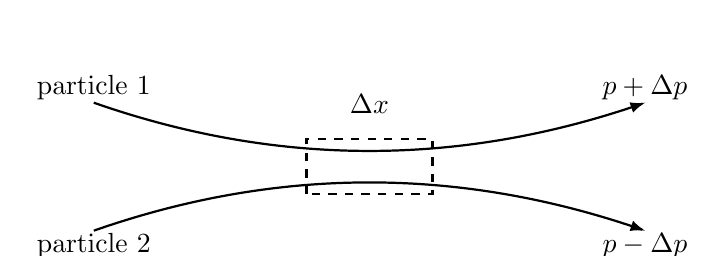
\begin{tikzpicture}[x=1cm,y=1cm,>=latex]


  % Two "wide" parabolas: one opening up, one opening down
  % Tune coefficients to make them "less curved" (small curvature).
  \draw[thick,->]
    plot[domain=0:7,samples=200]
    (\x,{0.05*(\x-3.5)^2 + 0.2});

  \draw[thick,->]
    plot[domain=0:7,samples=200]
    (\x,{-0.05*(\x-3.5)^2 - 0.2});

  % Region where they get close: dashed rectangle
  % Adjust these numbers to cover the "closest" part you want.
  \draw[dashed, thick] (2.7,-0.35) rectangle (4.3,0.35);
    \node at (0,1) {particle 1};
    \node at (0,-1) {particle 2};
    \node at (3.5,0.8) {$\Delta x$};
    \node at (7,1) {$p + \Delta p$};
    \node at (7,-1) {$p - \Delta p$};
\end{tikzpicture}
\caption{If spatial resolution is good enough to distinguish the two particles well enough, then we can not say which one goes up and down after the scattering. Also, if the momentum resolution is good enough}
\end{figure}
\section{Bosons and Fermions}

Consider $N$ identical particles (e.g., electrons, $\pi$ mesons). The Hamiltonian 
\begin{align}
    \oH = \oH(\xi_1,\xi_2,\dots,\xi_N)
\end{align}
is symmetric in the variables $\xi_1,\xi_2,\dots$. Here these variables includes position and spin degrees of freedom ($\bfvec{x}_i,\chi_{i}$ for $i=1,2,\dots,N$)\footnote{Even some other internal degrees of freedom such as isospin, color, flavor}. Likewise, we write a wave function in the form 
\begin{align}
    \psi = \psi(\xi_1,\xi_2,\dots,\xi_N)
\end{align}

Define a permutation operator (also called exchange operator) $\oP_{ij}$ as an operator that, when acting on an arbitrary $N-$particle wave function is 
\begin{align}
    \oP_{ij} \psi(\xi_1,\dots,\xi_i,\dots,\xi_j,\dots,\xi_N) = \psi(\xi_1,\dots,\xi_j,\dots,\xi_i,\dots,\xi_N)
\end{align}
By this we can see
\begin{align}
    \oP_{ij}^2 \psi(\dots) = \oP_{ij} \psi(\dots, i \leftrightarrow j) = \psi(\dots)
\end{align}
which means that\footnote{But we must be careful, the operator act the whole Hilbet space, such that this result is always true }
\begin{align}
    \oP^2_{ij} = \oI 
\end{align}
The eigenvalue of the permutation operator is $\pm 1$, which is obtained from following:
\begin{align*}
    &\oP_{ij} \phi = \lambda \phi \quad \forall \phi \neq 0 \\
   \implies& \oP^2{ij} \phi = \phi = \lambda^2 \phi  \\
    \implies & \lambda^2 = 1 , \quad \lambda = \pm1 \\
    \implies &\oP_{ij} \psi(\xi_1,\dots,\xi_i,\dots,\xi_j,\dots \xi_N) = \pm \psi(\xi_1,\dots,\xi_i,\dots,\xi_j,\dots \xi_N)
\end{align*}
Such that we can find that the eigenfunctions corresponding to the eigenvalue of $+1$ are symmetric and those corresponding to $-1$ corresponding to $-1$ are antisymmetric with respect to interchange of the pair $(i,j)$. Denoting by $\psi_{s} $ and $\psi_a$
\begin{align}
    \psi_s (\xi_1,\dots,\xi_i,\dots,\xi_j,\dots,\xi_N) &= + \psi_s (\xi_1,\dots,\xi_j,\dots,\xi_i,\dots,\xi_N) \\
    \psi_a (\xi_1,\dots,\xi_i,\dots,\xi_j,\dots,\xi_N) &= - \psi_a (\xi_1,\dots,\xi_j,\dots,\xi_i,\dots,\xi_N)
\end{align}

As we have discussed before,  identical particles are indistinguishable. Such that if the permutation of two particles does not change the physical observables, this implies that the Hamiltonian is symmetric with respect to the interchange of any pair of particles, i.e., $\comm{\oH}{\oP_{ij}} = 0$.
\paragraph{Properties of the permutation operator}
\begin{enumerate}
    \item If $\psi(\xi_1,\dots , \xi_N)$ is an eigenfunction of $\oH$ with eigenvalue $\oH$ with eigenvalue $E$, then the same also holds for $\oP_{ij} \psi(\xi_1,\dots,\xi_N)$.
    \begin{proof}
        \begin{align*}
            \oH \oP_{ij} \psi &= \oP_{ij} \oH \psi \\
            &= E \oP_{ij} \psi
        \end{align*}
    \end{proof}
    \item For every permutation one has 
    \begin{align}
        \braket{\Phi|\Psi} = \bra{\Phi} \oP_{ij}^\dagger \oP_{ij} \ket{\Psi} = \braket{\oP_{ij} \Phi | \oP_{ij} \Psi}
    \end{align}
    This comes from the fact that the permutation operator just changes the labels of the integration variables in the inner product integral. This also indicates that the permutation operator is unitary, i.e.,
    \begin{align}
        \oP_{ij}^\dagger \oP_{ij} = \oI
    \end{align}
    \item For every symmetric operator $\oS(\xi_1,\dots,\xi_N)$ we have 
    \begin{align}
        \comm{\oS}{\oP_{ij}} = 0
    \end{align}
    and 
    \begin{align}
        \bra{\psi_i} \oS \ket{\psi_j} = \bra{\oP_{ij} \psi_i} \oS \ket{\oP_{ij} \psi_j}
    \end{align}
\end{enumerate}

If we say that the particles are indistinguishable, then the physical observables should not change under the action of the permutation operator, consider two particles, with two observables $\oA_1$ and $\oA_2$, 

\begin{align}
    \oP_{ij} \oA \oP_{ij} = \oA
\end{align}
This implies that the Hamiltonian commutes with the permutation operator,
\begin{align}
    [\oH, \oP_{ij}] = 0
\end{align}

Particles described by symmetric wave functions are called bosons, while those described by antisymmetric wave functions are called fermions. Examples of bosons include photons, W and Z bosons, gluons, and the Higgs boson. Examples of fermions include electrons, protons, neutrons, and quarks.
















%\chapter{Topological Quantum Matter}   

\section{Berry Phase}



\section{Hall Conductance and Chern Numbers}

\section{Classification of Tologogical matter}

It is imporatnt to classify the type of topological 
\begin{align*}
    \nu = \frac{1}{2 \pi} \int_{[s]} \{  \}
\end{align*}

\begin{table}
    \centering
    \begin{tabular}{c|c|c}
    \hline
    s & s & s\\
    \hline
    \end{tabular}
\end{table}


%\chapter{Path Integral Formulation}
%\chapter{Quantum Matter}

This chapter fully based on the content of lecture "Quantum Matter" taught by Professor Johannes Deiglmayr in Leipzig University in 2026.
\section{Review of atomic physics}
\subsection{Emission and Absorption of Electromagnetic Radiation by Atoms}
\paragraph{Indued and Spontaneous emission}
If an atom in the state $\ket k$ with energy $E_k$ is brought into an electromagnetic radiation field with spectral energy density $\omega_{\nu}(\nu)$ (field energy per unit volume and unit frequency interval $\Delta \nu = 1\mathrm{s}^{-1}$) it can absorb a photon $h \nu$, which brings the atom into a state with higher energy $E_{f}=E_{k}+ h \nu$.

The probability 




The energy of photon to excited the electron does not need to be exactly the same as the energy difference between the two levels, but there is a width of the absorption spectrum, which is called the natural linewidth. The natural linewidth is determined by the lifetime of the excited state, which is related to the uncertainty principle. The shorter the lifetime, the broader the linewidth. The natural linewidth can be calculated using the formula:
\begin{align}
\Gamma = \frac{\hbar}{\tau}
\end{align}
\section{Laser Cooling and Trapping}
\subsection{Deceleration of an Atomic Beam}

\section{Atomic Bose-Einstein Condensates and degenerate Fermi Gas}

\section{Optical Dipole Traps, optical lattice and application in quantum simulation}

\section{Precision measurements of fundamental constants/atomic clock}
%\chapter{Anyons}

\section{Fractional Statistics in Two Dimensions}

As we already know that spin is quantized in integer or half-integer units, particles are divided into two kinds: fermions and bosons






























%\chapter{Diagrammatic perturbation theory}
\appendix

\chapter{Special Functions and Useful Formulas}

\section{Special Functions}

\subsection{Hyperbolic Functions}
The hyperbolic functions are defined as follows:
\begin{align}
    \sinh x & = \frac{\ee^x - \ee^{-x}}{2} \\
    \cosh x & = \frac{\ee^x + \ee^{-x}}{2} \\
    \tanh x & = \frac{\sinh x}{\cosh x} = \frac{\ee^x - \ee^{-x}}{\ee^x + \ee^{-x}}
\end{align}

The diagram below shows the graphs of the hyperbolic functions $\sinh x$, $\cosh x$ and $\tanh x$.
\begin{figure}[h!]
    \centering
    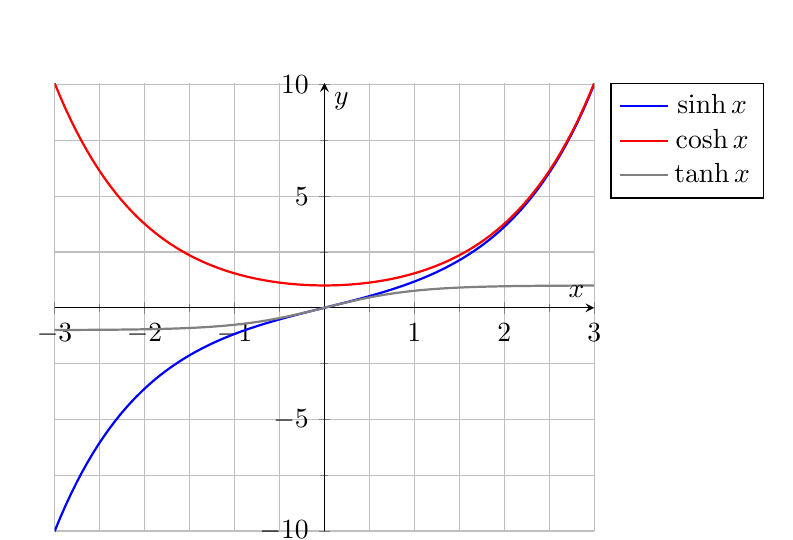
\begin{tikzpicture}
        \begin{axis}[
            axis lines = center,
            xlabel = {$x$},
            ylabel = {$y$},
            domain=-3:3,
            samples=100,
            legend pos=outer north east,
            grid=both,
            minor tick num=1,
        ]
        \addplot [blue, thick] {sinh(x)};
        \addlegendentry{$\sinh x$}
        
        \addplot [red, thick] {cosh(x)};
        \addlegendentry{$\cosh x$}
        
        \addplot [gray, thick] {tanh(x)};
        \addlegendentry{$\tanh x$}
        \end{axis}
    \end{tikzpicture}
    \caption{Graphs of Hyperbolic Functions}
    \label{fig:hyperbolic_functions}
\end{figure}

From whis we can easily see that $\cosh x$ is even function while $\sinh x$ and $\tanh x$ are odd functions. The domain of $\sinh x$ and $\cosh x$ is $(-\infty, +\infty)$ while the domain of $\tanh x$ is $(-\infty, +\infty)$ but the range is $(-1, 1)$. There are more useful identities involving hyperbolic functions:
\begin{align}
    \cosh^2 x - \sinh^2 x & = 1 
\end{align}
This can be proved easily by plugging in the definitions of $\sinh x$ and $\cosh x$. Also the derivatives of hyperbolic functions are:
\begin{align}
    \frac{\dd}{\dd x} \sinh x & = \cosh x \\
    \frac{\dd}{\dd x} \cosh x & = \sinh x \\
    \frac{\dd}{\dd x} \tanh x & = \frac{1}{\tanh^2 x} x
\end{align}
Additiaonally, the double-angle formulas are:
\begin{align}
    \sinh 2x & = 2 \sinh x \cosh x \\
    \cosh 2x & = \cosh^2 x + \sinh^2 x = 2 \cosh^2 x - 1 = 1 + 2 \sinh^2 x \\
    \tanh 2x & = \frac{2 \tanh x}{1 + \tanh^2 x}
\end{align}
angle sumation and half-andgle formulas are 
\begin{align}
    \sinh (x \pm y) & = \sinh x \cosh y \pm \cosh x \sinh y \\
    \cosh (x \pm y) & = \cosh x \cosh y \pm \sinh x \sinh y \\
    \tanh (x \pm y) & = \frac{\tanh x \pm \tanh y}{1 \pm \tanh x \tanh y} \\
    \sinh \frac{x}{2} & = \pm \sqrt{\frac{\cosh x - 1}{2}} \\
    \cosh \frac{x}{2} & = \pm \sqrt{\frac{\cosh x + 1}{2}} \\
    \tanh \frac{x}{2} & = \frac{\sinh x}{\cosh x + 1} = \frac{\cosh x - 1}{\sinh x}
\end{align}



\clearpage
\chapter{Group Theory Basics} \label{chap:GroupTheory}
 

\section{Definition of a Group}

\begin{definition}[Group]
    Let $G$ be a set on which a binary operation $G \times G \ra G$ is defined. $G$ is called a group iff the followind holds:
    \begin{itemize}
        \item \emph{Associativity}: $(g_1 \cdot g_2) \cdot g_3 = g_1 \cdot (g_2 \cdot g_3), \forall g_1, g_2, g_3 \in G$
        \item \emph{Identity Element}: There exists an element $e \in G$ such that $e \cdot g = g \cdot e = g, \forall g \in G$
        \item \emph{Inverse Element}: For each $g \in G$, there exists an element $g^{-1} \in G$ such that $g \cdot g^{-1} = g^{-1} \cdot g = e$
    \end{itemize}
\end{definition}
\begin{ex}
    \begin{itemize}
        \item
        \item The integers $\Z$ form a group with respect to the binary operation of addition, denoted by $(\Z,+)$. The unit element is given by $0$, and the inverse of $n$ is $-n$, $\forall n \in \Z$.
        \item The integers $\Z$ are not a group with respect to the binary operation of multiplication, denoted by $(\Z, \times)$. This is because not every element has an inverse in $\Z$; for example, there is no integer $m$ such that $2 \times m = 1$.
        \item The rotation group of 3d space $O(3) = \left\{O \in M_3(\R)\right\}$\footnote{$M_n(\cdot)$ denotes a $n \times n$ matrix with entries from the set in the parentheses.} with respect to the binary operation of matrix multiplication is a group. The unit element is given by the identity matrix $I_3$, and the inverse of a rotation matrix is its transpose.
    \end{itemize}
\end{ex}

\begin{definition}[Basic definitions:]
    \begin{itemize}
        \item A group $G$ is called \emph{finite, discrete} or \emph{continuous} depending on whether the set $G$ is finite, discrete (isomorphic to $\Z$) or uncountable.
    \end{itemize}
\end{definition}



\section{Lie Algebra, Lie Group, Basics of representation theory}
For translations, the generator is the momentum operator $\op$, which commutes with itself in different directions, i.e.,
\begin{align}
    \comm{\op_i}{\op_j} = 0 \quad \text{for } i,j = x,y,z
\end{align}
For rotations, the generator is the angular momentum operator $\oL$, which does not commute with itself in different directions, i.e.,
\begin{align}
    \comm{\oL_i}{\oL_j} = \ii \hbar \epsilon_{ijk} \oL_k \quad \text{for } i,j,k = x,y,z
\end{align}
\begin{definition}[Lie Algebra]
    \begin{enumerate}
        \item A Lie algebra $\mathfrak{g}$ is a real vector space. 
        \item Within $\mathfrak{g}$, there exists a bilinear, scew-symmetric map 
    \end{enumerate}
\end{definition}



\section{Representations of a Group} \label{sec:GroupRepresentations}






\chapter{Spherical Harmonics}

\section{Agular Momentum in Spherical Coordinates}

\subsection{General Expressions} \label{sec:AngularMomentum_SphericalCoord}
The Cartesian coordinates $(x,y,z)$ of a vector $\bfvec{r}$ are related to its spherical coordinates $(r,\theta,\phi)$ by 
\begin{align}
    x & = r \sin \theta \cos \phi \\
    y & = r \sin \theta \sin \phi \\
    z & = r \cos \theta
\end{align}
The orthonormal basis vectors in spherical coordinates $(\hat{\ee}_ r, \hat{\ee}_ \theta, \hat{\ee}_ \phi)$ are related to those in Cartesian coordinates $(\hat i ,\hat j, \hat k)$ by
\begin{align}
    \hat{\ee}_ r & = \sin \theta \cos \phi \hat i + \sin \theta \sin \phi \hat j + \cos \theta \hat k \\
    \hat{\ee}_ \theta & = \cos \theta \cos \phi \hat i + \cos \theta \sin \phi \hat j - \sin \theta \hat k \\
    \hat{\ee}_ \phi & = -\sin \phi \hat i + \cos \phi \hat j
\end{align}
Relove these equations, we have
\begin{align}
    \hat i & = \sin \theta \cos \phi \hat{\ee}_ r + \cos \theta \cos \phi \hat{\ee}_ \theta - \sin \phi \hat{\ee}_ \phi \\
    \hat j & = \sin \theta \sin \phi \hat{\ee}_ r + \cos \theta \sin \phi \hat{\ee}_ \theta + \cos \phi \hat{\ee}_ \phi \\
    \hat k & = \cos \theta \hat{\ee}_ r - \sin \theta \hat{\ee}_ \theta
\end{align}
Differentiating these equations, we obtain
\begin{align}
    \dd \hat{\ee}_ r & = \hat{\ee}_ \theta \dd \theta + \hat{\ee}_ \phi \sin \theta \dd \phi \\
    \dd \hat{\ee}_ \theta & = -\hat{\ee}_ r \dd \theta + \hat{\ee}_ \phi \cos \theta \dd \phi \\
    \dd \hat{\ee}_ \phi & = -\hat{\ee}_ r \sin \theta \dd \phi - \hat{\ee}_ \theta \cos \theta \dd \phi
\end{align}
From these, we can derive the component derivatives in spherical coordinates:
\begin{align}
    \pdv{r}{x} & = \sin \theta \cos \phi, & \pdv{r}{y} & = \sin \theta \sin \phi, & \pdv{r}{z} & = \cos \theta \\
    \pdv{\theta}{x} & = \frac{\cos \theta \cos \phi}{r}, & \pdv{\theta}{y} & = \frac{\cos \theta \sin \phi}{r}, & \pdv{\theta}{z} & = -\frac{\sin \theta}{r} \\
    \pdv{\phi}{x} & = -\frac{\sin \phi}{r \sin \theta}, & \pdv{\phi}{y} & = \frac{\cos \phi}{r \sin \theta}, & \pdv{\phi}{z} & = 0
\end{align}
From these we can find 
\begin{align}
    \pdv{}{x} & = \sin \theta \cos \phi \pdv{}{r} + \frac{\cos \theta \cos \phi}{r} \pdv{}{\theta} - \frac{\sin \phi}{r \sin \theta} \pdv{}{\phi} \\
    \pdv{}{y} & = \sin \theta \sin \phi \pdv{}{r} + \frac{\cos \theta \sin \phi}{r} \pdv{}{\theta} + \frac{\cos \phi}{r \sin \theta} \pdv{}{\phi} \\
    \pdv{}{z} & = \cos \theta \pdv{}{r} - \frac{\sin \theta}{r} \pdv{}{\theta}
\end{align}

Such that the gradient, Laplacian, is clear to be expressed 
\begin{align}
    \nabla = \hat i \pdv{}{x} + \hat j \pdv{}{y} + \hat k \pdv{}{z} = \hat{ee}_r \pdv{}{r} + \hat{\ee}_ \theta \pdv{}{\theta}
\end{align}
\section{Basics of Spherical Harmonics}


\section{Associated Legendre Functions} \label{sec:AssociatedLegendreFunctions}






%\printbibliography
\end{document}